%!TEX TS-program = xelatex
%!TeX spellcheck = en_GB
%!BIB TS-program = biber
\documentclass[paper=a4, fontsize=11pt, twoside, parskip=half, parskip=relative]{scrbook} 
%\documentclass[paper=a4, fontsize=11pt, twoside, parskip=half, parskip=relative,parnumber=true]{scrbook} 

	% double line
	%\documentclass[paper=a4, fontsize=12pt, twoside, parskip=half]{scrbook}% enabledeprecatedfontcommands is an option used for \rm


% ══════════════════════════════════════════════════════════════════════════════════════════════════
\def\mytitle{Computational Modelling of Fibre-Reinforced Composites\\[0.1cm]\LARGE and Nanocomposites}
\def\myauthor{Zia Javanbakht\\[0.1cm] {\small B.Sc., M.Sc.}}
\def\mydate{November 2019}
% ══════════════════════════════════════════════════════════════════════════════════════════════════

% this path points where style, figure, and video folders are located
\def\sourcefolder{.}

% Packages and macros
% My packages
% ──────────────────────────────────────────────────────────────────────────────────────────────────
% My Packages 
% ──────────────────────────────────────────────────────────────────────────────────────────────────


\newif\ifdouble
\doublefalse




% package for speeding up the compilation (I tried it did not work with the xr-hyper)
%\usepackage{subfiles}
%\usepackage{xr-hyper}

% ══════════════════════════════════════════════════════════════════════════════════════════════════
% Misc. packages
% ══════════════════════════════════════════════════════════════════════════════════════════════════
\usepackage{etex}                                % Solves the problem of too many packages
\usepackage{comment}                             % Defines the comment environment
\usepackage{makeidx}                             % allows index generation
%\usepackage{footnote}
\usepackage[bottom]{footmisc}                    % places footnotes at page bottom
\usepackage{datetime2}                           % date and time
\usepackage{enumitem}                            % flexibile options for enumerate env.


\iffig

\else
	 % geometry of the page
%    \usepackage[xetex, margin=3cm, a4paper]{geometry}                           
\fi


% ══════════════════════════════════════════════════════════════════════════════════════════════════
% Input and encoding
% ══════════════════════════════════════════════════════════════════════════════════════════════════
\usepackage[english]{babel}                      % Typographical and hyphenation
%\usepackage[latin1]{inputenc}                      % Accepts ISO Latin-1 encoding (only PDFTeX)


%\usepackage[T1]{fontenc}                         % The output can be easily copy pasted
\usepackage{lscape}                              % landscape env.
%\usepackage{layout}                              % Allows changing the layout of the page

\usepackage{scrhack}                              % load before setspace for corrections



% This package replaces lstlistings for xelatex engine. 
% minted uses Python pygments library, so you need to:
%    - Install Python, choose any version you like: x64 or x86, it better to choose 2.7.5 version.
%    - Add Python to PATH: C:\Python27;C:\Python27\Scripts
%    - pip install pygments to install Pygments 
\usepackage[cache=false]{minted}


%
%
%\ifdouble
%	\usepackage[doublespacing]{setspace}                             % different line spacings
%	% double spacing
%	\RedeclareSectionCommand[
%	  beforeskip=-1sp,
%	  afterskip=2\baselineskip]{chapter}
%	\RedeclareSectionCommand[
%	  beforeskip=-\baselineskip,
%	  afterskip=0.25\baselineskip]{section}
%	\RedeclareSectionCommand[
%	  beforeskip=-.75\baselineskip,
%	  afterskip=0.25\baselineskip]{subsection}
%	\RedeclareSectionCommand[
%	  beforeskip=-.5\baselineskip,
%	  afterskip=0.25\baselineskip]{subsubsection}
%	\RedeclareSectionCommand[
%	  beforeskip=.5\baselineskip,
%	  afterskip=-1em]{paragraph}
%	\RedeclareSectionCommand[
%	  beforeskip=-.5\baselineskip,
%	  afterskip=-1em]{subparagraph}
%	
%	  \setlist[enumerate,itemize]{
%	                              topsep    = 0.25\parskip,
%	                              itemsep   = 0.25\parskip,
%	                              partopsep = 0.25\parskip,
%	                              parsep    = 0.25\parskip
%	                             }
%\else
%	% Setting the spacing after/before sections
%	% normal spacing values
%	\RedeclareSectionCommand[
%	  beforeskip=-1sp,
%	  afterskip=2\baselineskip]{chapter}
%	\RedeclareSectionCommand[
%	  beforeskip=-\baselineskip,
%	  afterskip=0.5\baselineskip]{section}
%	\RedeclareSectionCommand[
%	  beforeskip=-.75\baselineskip,
%	  afterskip=0.5\baselineskip]{subsection}
%	\RedeclareSectionCommand[
%	  beforeskip=-.5\baselineskip,
%	  afterskip=0.5\baselineskip]{subsubsection}
%	\RedeclareSectionCommand[
%	  beforeskip=.5\baselineskip,
%	  afterskip=-1em]{paragraph}
%	\RedeclareSectionCommand[
%	  beforeskip=-.5\baselineskip,
%	  afterskip=-1em]{subparagraph}
%	
%	  \setlist[enumerate,itemize]{
%	                              topsep    = 0.5\parskip,
%	                              itemsep   = 0.25\parskip,
%	                              partopsep = 0.5\parskip,
%	                              parsep    = 0.5\parskip
%	                             }
%\fi


% Centering the subsection title
%\makeatletter
%\renewcommand{\sectionlinesformat}[4]{%
%  \ifstr{#1}{section}{\centering}{}% center section titles
%  \@hangfrom{\hskip #2#3}{#4.}%
%}
%\makeatother


% Adding a dot 
%\renewcommand{\sectioncatchphraseformat}[4]{%
%  \hskip #2#3#4%
%  \ifstr{#1}{subsubsection}{.}{}% dot after subsection titles
%}
%\renewcommand{\sectioncatchphraseformat}[4]{%
%  \hskip #2#3#4%
%  \ifstr{#1}{paragraph}{.}{}% dot after subsection titles
%}
%  
%
%




% ══════════════════════════════════════════════════════════════════════════════════════════════════
% Fonts
% ══════════════════════════════════════════════════════════════════════════════════════════════════
%\usepackage{helvet}                              % helvetica font loaded
%\usepackage{courier}                             % courier font loaded
%\usepackage{mathptmx}                            % times new roman font loaded for math (for tensors remove this)
%\usepackage{parskip}
\usepackage{type1cm}                              % removes the restriction on font scaling
\usepackage{ragged2e}                             % justifying the text
\usepackage{fontspec}

% Add a font that is not under the system fonts
%\fontspec [ Path            = ./_Fonts/,
%%UprightFont = *-regular,
%% BoldFont = *-bold
% Extension       = .otf,
% ]
%{FontAwesome}

                
    
\usepackage{fontawesome}                          % web fonts

%\setmonofont[                                     % Monospace font
%             Scale=0.8,
%             Path = ./_Fonts/
%            ]{DejaVuSansMono.ttf}                 
%\setmainfont[                                     % Text font
%             Ligatures={Common}, %Numbers={OldStyle}, Variant=01,
%             Path = ./_Fonts/,
%             BoldFont=LinLibertine_RB.otf,
%             ItalicFont=LinLibertine_RI.otf,
%             BoldItalicFont=LinLibertine_RBI.otf
%            ]{LinLibertine_R.otf}

%\setmonofont[Scale=0.9]{SFMono-Bold.otf}
    
    % Monospaced font
    \setmonofont{LibertinusMono-Regular.otf}[
                 Scale=0.8,
                 Path            = ./_Fonts/,
                 Extension       = .otf,
                ]                
    
    % Main text font
    \setmainfont{LibertinusSerif}[%
                 Ligatures       = {Common}, %Numbers={OldStyle}, Variant=01,
                 Path            = ./_Fonts/,
                 Extension       = .otf,
                 UprightFont     = *-Regular,
                 BoldFont        = *-Bold,
                 ItalicFont      = *-Italic,
                 BoldItalicFont  = *-BoldItalic,
                ]
    % Sanserif font
    \setsansfont{LibertinusSans}[
                 Path            = ./_Fonts/,
                 Extension       = .otf,
                 UprightFont     = *-Regular,
                 BoldFont        = *-Bold,
                 ItalicFont      = *-Italic,
                ]
    




%\setmainfont{Times New Roman}

% ══════════════════════════════════════════════════════════════════════════════════════════════════
% Math
% ══════════════════════════════════════════════════════════════════════════════════════════════════

%\usepackage{amsmath}                             % main math environment (always before unicode-math)
\usepackage{mathtools}                            % extension to amsmath which loads it automatically
\usepackage{amsthm}                               % math theorems
\usepackage{mathrsfs}
%\usepackage{amssymb}                             % symbols like \square  (always before unicode-math)
\usepackage{xfrac}                                % slanted fractions 
\usepackage{accents}
%\usepackage[bb=mma,cal=cm,scr=esstix]{mathalfa}
\usepackage{unicode-math}                        % Math for XeLaTeX
\usepackage{stackrel}                             % Enhancements to the \stackrel command


\unimathsetup{math-style=ISO, bold-style=ISO}




    % Math font setting
    \setmathfont{LibertinusMath-Regular}[             % General math font
                 Path            = ./_Fonts/,
                 Extension       = .otf
                 ]
    
    % Requires lm-math package
    \setmathfont{Latin Modern Math}[                  % Calligraphy font for linear operators
                 range           = {cal, bfcal},
                 ]
    
    % Requires tex-gyre-math package
    \setmathfont{TeX Gyre Termes Math}[               % For proper blackboard letters
                 range=bb
                 ]
    
    \setmathfont{XITSMath-Regular}[               % For fraktur
                 Path            = ./_Fonts/,
                 Extension       = .otf,
                 range           = frak,
                 ]
    
    \setmathfont{XITSMath-Bold}[               % For fraktur
                 Path            = ./_Fonts/,
                 Extension       = .otf,
                 range           = bffrak,
                 ]
    
    
    \setmathfont{LibertinusMath-Regular}[             % For upright Greek letters using \mup...
                 Path            = ./_Fonts/,
                 Extension       = .otf,
                 range           = up/{greek,Greek},          
                 math-style      = literal
                 ]
    
    




% Working math fonts
%\setmathfont{Latin Modern Math}
%\setmathfont{XITSMath-bold.otf}[Path = ./_Fonts/,range=bfcal,StylisticSet=1]


%% do not remember what are these two lines for
%\setmathfont{XITSMath-bold.otf}[range=bfgre,StylisticSet=1]
%\setmathfont[range=bb]{Linux Libertine O}







\usepackage{textcase}                            % creeating upper and lower case letters
\usepackage{mathtools}
\usepackage{pifont}

\usepackage{cancel}

%\usepackage{calrsfs} 
%\usepackage{mathrsfs}                            % Styles for MATH mode
%\usepackage{dutchcal}

%\usepackage{epstopdf}





	% Defining new float environments
	\usepackage{newfloat}




% ══════════════════════════════════════════════════════════════════════════════════════════════════
% Setting the chapter style for Komma
% ══════════════════════════════════════════════════════════════════════════════════════════════════
\ifdouble

% Change the chapter style
\renewcommand{\chapterlinesformat}[3]{%
\vspace{0.1\textheight}% space between the chapter number and the line
\raisebox{-0.5\baselineskip}{\parbox[c][15pt]{\linewidth}{#2}}
\rule{\textwidth}{4pt}
\parbox[c][45pt]{\dimexpr\linewidth-2\fboxrule-2\fboxsep}{\mdseries\scshape\fontsize{20}{14}\selectfont#3}\\
\rule{\textwidth}{4pt}\vspace{0.1\textheight}
}

% Change the chapter font
\addtokomafont{chapter}{\mdseries\fontsize{14}{10}\selectfont\scshape}

\else
%
%% Change the chapter style
%\renewcommand{\chapterlinesformat}[3]{%
%\vspace{0.05\textheight}
%\raisebox{-0.5\baselineskip}{\parbox[c][15pt]{\linewidth}{#2}}
%\rule{\textwidth}{4pt}
%\parbox[c][45pt]{\dimexpr\linewidth-2\fboxrule-2\fboxsep}{\mdseries\scshape\fontsize{26}{20}\selectfont#3}\\
%\rule{\textwidth}{4pt}\vspace{0.1\textheight}
%}
%
%% Change the chapter font
%\addtokomafont{chapter}{\mdseries\fontsize{18}{12}\selectfont\scshape}
%\fi
%
%
%
%
%% Change the number formating
%\renewcommand{\chapterformat}{\chaptername\ \thechapter}
%


% Change the appendix style
\makeatletter
\g@addto@macro\appendix{%
  \renewcommand*{\chapterformat}{%
    {\chapapp\nobreakspace\thechapter\enskip}%
  }
  \renewcommand*{\chaptermarkformat}{%
    {\chapapp\nobreakspace\thechapter\enskip}%
  }
  \let\oldaddcontentsline\addcontentsline
  \newcommand\hackedaddcontentsline[3]{\oldaddcontentsline{#1}{#2}{\chapapp\nobreakspace#3}}
%  \let\oldchapter\chapter
%  \renewcommand*\chapter[1]{%
%    \let\addcontentsline\hackedaddcontentsline%
%    \oldchapter{#1}%
%    \let\addcontentsline\oldaddcontentsline%
%  }
}
\makeatother

% ══════════════════════════════════════════════════════════════════════════════════════════════════
% Formatting of the sections
% ══════════════════════════════════════════════════════════════════════════════════════════════════
%
%\addtokomafont{section}{\mdseries\normalfont\Large}
%\addtokomafont{subsection}{\large\mdseries\normalfont}
%\addtokomafont{subsubsection}{\mdseries\itshape\normalsize}
%
%% Change ToC to serif font
%\setkomafont{disposition}{\normalfont\bfseries}     

% ══════════════════════════════════════════════════════════════════════════════════════════════════
% Symbols
% ══════════════════════════════════════════════════════════════════════════════════════════════════
%\usepackage{upgreek}                             % upright greek letter
\usepackage[normalem]{ulem}                      % Various underlinings
\usepackage{marvosym}                            % adds some symbols, e.g., CheckedBox
\usepackage{manfnt}                              % symbols from Knuth's TeX manual
\usepackage{wasysym}                             % adds some symbols, e.g., CheckedBox
\usepackage{tikzsymbols}                         % tree symbol

% ══════════════════════════════════════════════════════════════════════════════════════════════════
% Tables
% ══════════════════════════════════════════════════════════════════════════════════════════════════
\usepackage{array}                               % extended capabilities to tabular env.
\usepackage{booktabs}                            % toprule, bottomrule, midrule etc.
\usepackage{colortbl}                            % color rows and columns for tables
\usepackage{multicol, multirow}                  % used for the two-column index
\usepackage{longtable}
\usepackage{siunitx}							 % SI units + s-type tabular data
\usepackage[skip=0em,
            belowskip=1em,
            aboveskip=1em,
            labelfont=bf                         % use bold caption labels
            ]{caption}                           % placement of caption of the floats is fine-tuned

\setlength{\aboverulesep}{0pt}                   % these two lines are to remove the gap 
\setlength{\belowrulesep}{0pt}                   % in the color tables when toprule and bottomrule is used
\setlength{\extrarowheight}{.75ex}

% ══════════════════════════════════════════════════════════════════════════════════════════════════
% Figures
% ══════════════════════════════════════════════════════════════════════════════════════════════════
%\usepackage{subfigure}                          % using multiple subfigures in figure (obsolete)
%\usepackage{subcaption}                         % using multiple subfigures in figure (obsolete)
\usepackage{subfig}                              % better alternative !

\usepackage{hhline}
%\setlength{\extrarowheight}{.5ex}
% Graphics
\usepackage[export]{adjustbox}                           % frame for pictures
\usepackage{graphicx}                            % standard LaTeX graphics tool
\usepackage{xcolor}                              % used to introduce different colors



\usepackage{afterpage}                           % flush floats \afterpage{\clearpage}
%\usepackage{media9}                              % embeding .h264 format MP4 videos
%\usepackage{bohr}                                % draws elements
%\usepackage{chemformula}                         % for chemical formulas
%\usepackage{chemfig}                             % to draw chemicals
\usepackage[many]{tcolorbox}                          % for colored and framed text boxes
\tcbuselibrary{skins,xparse}
%\usepackage[color=commentcolor,author={Zia}]{pdfcomment}

\usepackage{mdframed}                            % gray box package and the theorem environment



%\lstset{basicstyle=\footnotesize\ttfamily,backgroundcolor=\color{black!10}}


% Programming
\usepackage{xpatch}                              % patching the biblatex package
\usepackage{ifpdf}                               % checks if PDFLaTeX is used


%\addtobeamertemplate{headline}{\hypersetup{linkcolor=blue}}{}
%\addtobeamertemplate{footline}{\hypersetup{linkcolor=.}}{}





	% hyperref must be loaded after all packages
    \usepackage[colorlinks = true,  
                linkcolor  = green!50!black, 
                urlcolor   = blue!75!green!75,
                citecolor  = blue!50!green,
                bookmarks]{hyperref}
	\hypersetup{pdfinfo	= 
					{	Author      	= {Zia Javanbakht},
                 		Subject     	= {Computational Modelling of Natural Fibre Composites, Phd Thesis},
						Institution 	= {Griffith University}
					}
				}
				
	% Customising section commands in a KOMA-script files (\usepackage{sectsty} for others)
    \usepackage[automark, headsepline]{scrlayer-scrpage}       

    \setlist[description]{                           % Setting for symbols and abbreviations
                          leftmargin    = 2.5cm,
                          labelindent   = 0.5cm,
                          labelwidth    = 2cm,
                          itemindent    = 0.5mm,
                          labelsep      = 0mm,
                          topsep        = 0em,
                          itemsep       = 0mm,
                          partopsep     = 1em,
                          parsep        = 0em,
                          listparindent = 0mm,
                         }   








% TikZ for drawings
\usepackage{pgfgantt}                            % used for gantt chart
%\usepackage{pgfplotstable}                      % loads all the pgf packages
\usepackage{pgfplots}                            % loads all the pgf packages
%\pgfplotsset{compat=1.7}                         % sets the version of pgfplots

\usepackage{tikz}
\usetikzlibrary{spy,fit,matrix,shapes.callouts,calc,trees,positioning,arrows,chains,shapes.geometric,shapes.multipart,arrows.meta,  decorations.pathreplacing,decorations.text,decorations.pathmorphing,decorations.markings,shapes,matrix,shapes.symbols,patterns,datavisualization,datavisualization.formats.functions,angles,backgrounds}


\usepackage[]{contour}                    % for outlining text

% ══════════════════════════════════════════════════════════════════════════════════════════════════
% Commands for picture environment
% ══════════════════════════════════════════════════════════════════════════════════════════════════


\endinput



% width and length of pic arrows
\newcommand{\picw}{0.13}
\newcommand{\picl}{0.25}

\tikzset{
 xaxis/.pic     ={\path[draw, fill,  pic actions] (0,0,0) -- ++(0,0,\picw/2) -- ++(\picl,0,-\picw/2)-- ++ (-\picl,0,-\picw/2) -- cycle;},
 xaxisflat/.pic ={\path[draw, fill,  pic actions] (0,0,0) -- ++(0,\picw/2,0) -- ++(\picl,-\picw/2,0)-- ++ (-\picl,-\picw/2,0) -- cycle;},
 yaxis/.pic     ={\path[draw, fill,  pic actions] (0,0,0) -- ++(0,0,\picw/2) -- ++(0,\picl,-\picw/2)-- ++ (0,-\picl,-\picw/2) -- cycle;},
 yaxisflat/.pic ={\path[draw, fill,  pic actions] (0,0,0) -- ++(\picw/2,0,0) -- ++(-\picw/2,\picl,0)-- ++ (-\picw/2,-\picl,0) -- cycle;}, 
 zaxis/.pic     ={\path[draw, fill,  pic actions] (0,0,0) -- ++(0,\picw/2,0) -- ++(0,-\picw/2,\picl)-- ++ (0,-\picw/2,-\picl) -- cycle;},
 zaxisrot/.pic  ={\path[draw, fill,  pic actions] (0,0,0) -- ++(-\picw/2,0,0) -- ++(\picw/2,0,\picl)-- ++ (+\picw/2,0,-\picl) -- cycle;}
}

% ══════════════════════════════════════════════════════════════════════════════════════════════════
% tikz-3dplot settings
% ══════════════════════════════════════════════════════════════════════════════════════════════════
\usepackage{tikz-3dplot}

\setlength{\unitlength}{\textwidth*1/160}
\tdplotsetmaincoords{235}{-40}


% ══════════════════════════════════════════════════════════════════════════════════════════════════
% Global values for dimensions, arrows, etc. used in tikzpicture env.
% ══════════════════════════════════════════════════════════════════════════════════════════════════

% Dimensions of the plate
\newlength{\plx}
\newlength{\ply}
\newlength{\plt}

\setlength{\plx}{6pt}
\setlength{\ply}{6pt}
\setlength{\plt}{2pt}

% Arrow dimensions
\newlength{\annotdim}
\setlength{\annotdim}{5.5pt}

\newlength{\annottext}
\setlength{\annottext}{10pt}

% Force dimension
\newlength{\forcelen}
\setlength{\forcelen}{1.5pt}

\newlength{\baselen}
\setlength{\baselen}{1pt}


% Modified tdplotdrawarc to accomodate pic and extra nodes
\newcommand{\tdplotarc}[8][tdplot_main_coords]{%
\pgfmathsetmacro{\tdplottemp}{#5 + #4}
\tdplotdiv{\tdplottemp}{\tdplottemp}{2}
\path[#1] #2 + (\tdplottemp:#3) node[#6]{#7};
\draw[#1] #2 + (#4:#3) arc (#4:#5:#3) #8;
}




% ══════════════════════════════════════════════════════════════════════════════════════════════════
% Commands for TikZ
% ══════════════════════════════════════════════════════════════════════════════════════════════════

\def\splittedv#1{\nodepart[text width=0.1,inner sep=0]{one}  \nodepart[]{two} #1 \nodepart[text width=0.1]{three}}
\def\splittedh#1[#2]{\nodepart[text height=0.1cm,inner sep=0,rectangle split every empty part={},rectangle split empty part height=0.1cm,]{one} \nodepart[align=center,text width=1cm,#2]{two}#1}
% Flowchart styles
  \tikzset{
   %% Define styles for structural symbols
    %simple node
    snode/.style = {draw,thick,circle, text height = 0.2cm, text width= 0.2cm,inner sep=0, minimum size = 2mm },
    % elements
    myelement/.style = {draw,ultra thick},
    % point load
    pload/.style   = {draw, text width=2cm, rectangle, thick},
    %% Define styles for flowchart symbols
    % basic style
    fbase/.style = {draw, fill=lightgray, inner sep=1mm, semithick},
    % Node label style (plain text)
    nlabel/.style = {label=left:{\small#1}},
    % Process style (Rectangle)
    fproc/.style = {fbase, rectangle,text width=0.75cm},
    % I/O style (Parallelogram)
    fio/.style = {fbase, trapezium, trapezium right angle=120, trapezium left angle=60,text width=0.75cm},
    % Flowchart Connection style (arrows)
    fconc/.style = {semithick, draw,-stealth,label={"#1"}},
    % Simple Connection style (lines)
    sconc/.style = {semithick, draw,label={"#1"}},
    % Terminal style (ellipse)
    fterm/.style = {fbase, ellipse, inner sep=0.5mm},
    % Decision style (diamond)
    fdeci/.style = {fbase, diamond, inner sep=0mm, minimum size=0.3cm},
    % Extra info bracket style (bracket)
    fbrac/.style = {decorate, decoration=brace, thick},
    % Intrinsic subprogram style (Splited rectangle)
    fsubin/.style = {fbase,rectangle split, rectangle split parts=3, rectangle split horizontal,semithick,rectangle split empty part width=0.1cm, inner xsep=0.05cm, inner ysep=1mm},
    % External/internal subprogram (Splited rectangle from top)
    fsubex/.style = {fbase, inner sep=0,rectangle split,rectangle split every empty part={},rectangle split empty part height=0cm,rectangle split empty part width=0ex, rectangle split empty part depth=0cm,,rectangle split parts=2, semithick,text height=-0.3cm},
    % Callout style (comments)
    mycallout/.style = {draw,pattern=north west lines, pattern color=lightgray!75, semithick, rectangle callout, inner sep=2mm,align=justify,callout absolute pointer={#1},text width=4cm},
    % Junction style (small circles)
    fjunc/.style = {fbase, circle, inner sep=0mm,text width=1mm,,minimum size=2mm},
    % Off-page connector style (Trapezoid)
    fnext/.style = {fbase, inner xsep=1mm,inner ysep=0.5mm,chamfered rectangle,chamfered rectangle ysep=0.5cm,chamfered rectangle xsep=0.5cm,chamfered rectangle corners={south west,south east},text width=2mm},
    % Matrix style but outside of a matrix
    matrixoutstyle/.style ={draw,line width=0.75pt, anchor=center,fill=gray!50, text centered, rounded corners=0.1cm, minimum width=1cm, minimum height=5mm, minimum width=0.2cm,inner sep=1mm, font=\scriptsize},
    % General Matrix style
    matrixstyle/.style={matrix of nodes, nodes={matrixoutstyle},row sep=0.4cm, column sep=1cm, minimum width=0.2cm,inner sep=0, font=\scriptsize},
    % General tikzstyle
    mytikzstyle/.style={node distance=0.5cm,anchor=center,font=\scriptsize},
    % Pseudocode style
    pcstyle/.style={node distance=-0.15cm},
    % Flowchart style
    fcstyle/.style={row sep=0cm,column sep=0cm,minimum width=1mm,align=center},
    % Flowchart blank node
    fblanku/.style={yshift=0.4cm},
    fblankd/.style={yshift=-0.4cm},
    % To put a node between two others
    between/.style args={#1 and #2}{at = ($(#1)!0.5!(#2)$)}
  }



%\usepackage{flowchart}                          % Flowchart package (TIKZ is implicitly loaded by FLOWCHART package)

% My TikZ package
%\input{./_Style/FETikZ}

% Using customized BibLaTex
%%%%%%%%%%%%%%%%%%%%%%%%%%%%%%%%%%%
%%%% Notes on BibLaTex Package
%%%
%%
%
% There are four important files:
%  1. biblatex.bst
%  2. biblatex.def
%  3. biblatex.sty
%  4. standard.bbx
%  5. biblatex.bst which is used if the backend is set to bibtex.
%
% Natbib is another alternative for BibLaTeX
%   \usepackage[]{natbib}                           % used along with springer package
%   \setcitestyle{authoryear,round}
%   \setcitestyle{authoryear,round,sorted}
%
%
%

\usepackage[%
  bibencoding=ascii,
  giveninits=true, 
  sorting=nyt, 
  dateabbrev = false,
  doi=false,
  isbn=false,
  url=false,
  useprefix,
  terseinits=true,
  backend=biber,
  style=authoryear,
  uniquename=init
           ]{biblatex}
\usepackage{bibentry}
\usepackage[style=english]{csquotes}                            % this is recommended to be used with biblatex for quotations
\addbibresource{E:/#Science/Continuum Mechanics/My Thesis/_References/references.bib}
\addbibresource{E:/#Science/Continuum Mechanics/My Thesis/_References/paper4.bib}
\addbibresource{E:/#Science/Continuum Mechanics/My Thesis/_References/paper5.bib}



\DeclareNameAlias{sortname}{last-first}          % reverses the last/first name
\renewcommand*{\finalnamedelim}{%                % change the final delimiter to &
  \ifnumgreater{\value{liststop}}{2}{}{}%
  \addspace\&\space}%


% Change the font of the URLs
\renewcommand{\UrlFont}{\small\rm}

\renewrobustcmd*{\bibinithyphendelim}{}
\renewcommand{\labelnamepunct}{\addcomma\space}   % comma after year
\renewcommand{\subtitlepunct}{\addcolon\space}    % comma after year
\renewcommand{\newunitpunct}{\addcomma\space}     % punctuation after a \newunit command

\renewcommand{\newblockpunct}{}     % punctuation after a \newunit command


%%%%%% \xpretobibmacro{date+extrayear}{\setunit{\space}}{}{}


%\renewcommand*{\multinamedelim}{{{\color{red!80!black}\addsemicolon\addspace}}}



\renewbibmacro{in:}{}                            % remove `in' in every type of entry

% Swaping the location and publisher
\renewbibmacro*{publisher+location+date}{%
  \printlist{publisher}%
  \iflistundef{location}
    {\setunit*{\addcomma\space}}
    {\setunit*{\addcomma\space}}%
  \printlist{location}%
  \setunit*{\addcomma\space}%
  \usebibmacro{date}%
  \newunit}
% Removing parantheses around the yaer
\makeatletter
\def\act@on@bibmacro#1#2{%
  \expandafter#1\csname abx@macro@\detokenize{#2}\endcsname
}
\def\patchbibmacro{\act@on@bibmacro\patchcmd}
\def\pretobibmacro{\act@on@bibmacro\pretocmd}
\def\apptobibmacro{\act@on@bibmacro\apptocmd}
\def\showbibmacro{\act@on@bibmacro\show}
\makeatother

% this changes the abbreviated first name
\patchbibmacro{date+extrayear}{%
  \printtext[parens]%
}{%
  \setunit{\space}% this line is what appears after the last name field
  \printtext%
}{}{}


% Journal article

\DeclareFieldFormat[article]{volume}{\bibstring{jourvol}\addnbspace #1}
\DeclareFieldFormat*[article]{issue}{#1}


\renewbibmacro*{volume+number+eid}{%
  \addcomma\space
  \printfield{volume}%
  \setunit{\addcomma\space}%
  \newunit
  \printfield{number}%
  \printfield{eid}}
 
% removes the brackets around the issue number and puts no. before it.
\renewbibmacro*{issue+date}{%
    \iffieldundef{issue}
      {\usebibmacro{date}}
      {% if issue exists...
        \addcomma\space no.\addnbspace
        \printfield{issue}%
        \setunit{\addcomma\space}%
       \usebibmacro{date}}%
  \newunit}



\DefineBibliographyStrings{english}{%
    number = {\lowercase{v}ol\adddot}, % avoid capitalization after dots.
    issue  = {\lowercase{i}ss\adddot}, % avoid capitalization after dots.
}

%
% a unit is a field for a bibliographical item, e.g., for a book
% the following units are mandatory: author, title, and year/date.
% after each unit a \newunit command runs to add the proper punctuation
%


\DeclareFieldFormat[book]{title}{\mkbibemph{#1}}  % italic title for books


\DeclareFieldFormat{series}{#1}% publication series

\renewbibmacro*{title}{%
  \ifboolexpr{
    test {\iffieldundef{title}}
    and
    test {\iffieldundef{subtitle}}
  }
    {}
    {\printtext[title]{%
       \printfield[titlecase]{title}%
       \setunit{\subtitlepunct}%
       \printfield[titlecase]{subtitle}}%
     \newunit}%
  \printfield{titleaddon}}



%% For online source
\DeclareFieldFormat{url}{<\url{#1}>}
%\DeclareFieldFormat{urldate}{viewed\space#1}
\DeclareFieldFormat{urldate}{viewed\space\thefield{urlday}\addspace%
  \mkbibmonth{\thefield{urlmonth}}\addspace%
  \thefield{urlyear}}


\renewbibmacro{url+urldate}{%
  \usebibmacro{urldate}%
  \newunitpunct%
  \usebibmacro{url}%
}

%%% Defining a driver for the `standard' type
%
% sample bib item
%   @standard{s.2020,
%    title = {Tutoring code of practice},
%    url = {www.saiglobal.com},
%    urldate = {2020-01-01},
%    number = {HB201--2006},
%    abstract = {},
%    date = {2006},
%    author = {{Standards Australia}}
%   }
%
% The driver decleration is adopted from  standard.bbx
%
% example:
% Standards Australia International 2000, \textit{AS 1235-2000 Road vehicles: roof load carriers: roof bars}, 5th edn, standards, viewed 3 February 2012, http://infostore.saiglobal.com/store/Details.aspx?ProductID=218577
%

\DeclareBibliographyDriver{standard}{%
  \usebibmacro{bibindex}%
  \usebibmacro{begentry}%
  \usebibmacro{author}%
  \setunit{\labelnamepunct}\newblock
  \usebibmacro{title}%
  \newunit\newblock
  \printfield{number}%
  \setunit{\addspace\addcomma}\newblock\newunit%
  \addcomma\addspace standards\newunit%
  \iftoggle{bbx:url}
    {}
    {\usebibmacro{url+urldate}}%
  \usebibmacro{finentry}%
}


% misc type is used as wiki type 
\DeclareFieldFormat[misc]{title}{\mkbibquote{#1}}  % quotes title for wiki
\DeclareFieldFormat[misc]{year}{#1}  % quotes title for wiki


\DeclareBibliographyDriver{misc}{%
  \usebibmacro{bibindex}%
  \usebibmacro{begentry}%
%
  \iffieldundef{author}
  {% w/o author(s)
  \setunit{\addspace}%
  }
  {% w/t author(s)
  \usebibmacro{author}%
  \printdate%
  \setunit{\labelnamepunct\addspace}%
  }
  \printfield{title}%
  \iffieldundef{author}%
  {% w/o author(s)
  \printdate%
  }
  {% w/t author(s)
  }
  \setunit{\addcomma\addspace}%
  \printtext{\mkbibemph{Wikipedia}\addcomma\addspace}%
  \iftoggle{bbx:url}
    {}
    {\usebibmacro{url+urldate}}%
  \usebibmacro{finentry}%
}
%
% \newunit
%   finished the current unit,
%   puts \newunitpunct in the buffer
%   next print command prints the entire buffer after itself
%
% \setunit
%   finishes the current unit,
%   next print command prints the entire buffer after itself
%
% \setunit*
%   it runs / setunit provided that the last print command actually printed anything.
%
% \fineentry
%   at the end of every bibliographical item it must run and it 
%
% \newblock
%   records the end of the current block in the buffer
%   puts \newblockpunct 
%   a new block is automatically started after a printing command
%
% \printtext[text-format]{text}
%    prints {text} with the [text-format]
%    flushes the buffer
%    usually used for a piece of text rather than a field
%


%\DeclareFieldFormat
%  [article,inbook,incollection,inproceedings,patent,thesis,unpublished]
%  {title}{\makebibquote{#1}}

% My Customized Macros
%%%%%%%%%%%%%%%%%%%%%%%
%% Customized Macros %%
%%%%%%%%%%%%%%%%%%%%%%%

% Common macros
%%%%%%%%%%%%%%%%%%%
%% Common Macros %%
%%%%%%%%%%%%%%%%%%%

% Common settings for all lectures in this course
\def\mycampus{Gold Coast Campus}
\def\myuniversity{Griffith University}
\def\myschool{Griffith School of Engineering and Built Environment}
\def\mycoursename{Engineering Materials}
\def\mycoursecode{1017ENG}
\def\mycourse{\mycoursecode~\mycoursename}
\def\myinstitute{\myuniversity\par\myschool\par\mycampus}

% These two lines work for both beamer and non-beamer
\date{\mydate}
\title{\mytitle}


% Add blank page
\newcommand\blankpage{%
    \afterpage{\null
    \thispagestyle{empty}%
    \addtocounter{page}{-1}%
    \newpage}\clearpage}

% ══════════════════════════════════════════════════════════════════════════════════════════════════
% Abbreviations in smallcaps
% ══════════════════════════════════════════════════════════════════════════════════════════════════

% Marc in smallcaps
\def\m{\fontshape\scdefault\selectfont Marc\normalfont}
% Mentat in smallcaps
\def\M{\fontshape\scdefault\selectfont Mentat\normalfont}
% Marc/Mentat in smallcaps
\def\mm{\fontshape\scdefault\selectfont Marc/Mentat\normalfont}
% Fortran Code
\def\fc#1{\textsf{\small{#1}}}
% Fortran Code scriptsize
\def\fcscript#1{\textsf{\scriptsize{#1}}}
% KeyWords
\def\kw#1{\fc{\MakeTextUppercase{#1}}}
% KeyWords scriptsize
\def\kwscript#1{\fcscript{\MakeTextUppercase{#1}}}
% New Paragraph without indents
\def\np{\par\noindent}
% My Quotation 
\newcommand{\myquote}[2]{\begin{center}\begin{minipage}{0.6\textwidth}\emph{{#1}}\vspace{-0.3cm}\flushright{{\scriptsize%
\if\relax\detokenize{#2}\relax
Anonymous
\else
#2
\fi
}}\\\end{minipage}\end{center}}

% Fortran Code
  \def\fc#1{\textsf{#1}}
% Fortran Code scriptsize
\def\fcscript#1{\textsf{\scriptsize{#1}}}
% Fortran
\def\f{\fontshape\scdefault\selectfont Fortran\normalfont}
% Marc in smallcaps
\def\m{\fontshape\scdefault\selectfont Marc\normalfont}
% Mentat in smallcaps
\def\M{\fontshape\scdefault\selectfont Mentat\normalfont}
% Marc/Mentat in smallcaps
\def\mm{\fontshape\scdefault\selectfont Marc/Mentat\normalfont}
% Intel
\def\intel{\fontshape\scdefault\selectfont Intel{$^{\scaleobj{0.7}{\textregistered}}$}\normalfont} 
% Syntax


\newcommand{\code}[1]{\texttt{#1}}


% ══════════════════════════════════════════════════════════════════════════════════════════════════
% Symbols
% ══════════════════════════════════════════════════════════════════════════════════════════════════

\newenvironment{syntax}{\par\vspace{0.2cm}\sffamily\small}{\vspace{0.2cm}\normalfont\newline\noindent}%
% x mark
\newcommand{\xmark}{\ding{55}}
% Check mark
\newcommand{\cmark}{\ding{51}}
% My checkedBox
\def\myCheckedBox{\hbox{\raise.2em\hbox{\cmark}\kern-0.9em\hbox{$\square$}}}
% My CrossedBox
\def\myCrossedBox{\hbox{\hbox{\resizebox{1.2ex}{!}{\xmark}}\kern-0.7em\raise-.05em\hbox{$\square$}}}
% The tree
\def\thetree{\BasicTree[3.]{blue!80!red!40!white}{blue!80!red!30!white!30!black}{blue!70!red!60!white}{leaf}}
% The arrow
\def\thearrow{\resizebox{2.5em}{!}{\ding{224}}}
% The hand
\def\thehand{\resizebox{2.5em}{!}{\ding{45}}}

% ══════════════════════════════════════════════════════════════════════════════════════════════════
% Environments
% ══════════════════════════════════════════════════════════════════════════════════════════════════

% Summary box using mdframed
\newenvironment{summary}{%
\begin{mdframed}[middlelinewidth=2pt, backgroundcolor=gray!50, linecolor=white]%
\textbf{Summary}\quad
}{%
\end{mdframed}%
}



\makeatletter
	% For Koma-script, automatically add a full stop after the paragraph title
	



%
%% Defintition box using mdframed
%\newtheoremstyle{mystyle2}{0}{}{}{}{\bfseries}{:}{ }{\thmname{#1} \thmnumber{#2} --- \textbf{\thmnote{#3}}}
%\theoremstyle{mystyle2}
%\newmdtheoremenv[
%hidealllines        = true,
%leftline            = true,
%linewidth           = 4pt,
%linecolor           = gray!40,
%innerrightmargin    = 0pt,
%frametitleaboveskip = 0mm,
%frametitlebelowskip = 0mm,
%skipabove           = \baselineskip,
%skipbelow           = \baselineskip,
%splittopskip        = 0mm,
%innerbottommargin   = 0pt,
%innertopmargin      = 0.75\baselineskip,
%]{definition}{Definition}[chapter]
%
%\renewcommand{\thedefinition}{\arabic{chapter}.\arabic{definition}}
%
%% Theorem box using mdframed
%\newtheoremstyle{mystyle1}{0}{}{}{}{\bfseries}{:}{ }{\thmname{#1} \thmnumber{#2} --- \textbf{\thmnote{#3}}}
%\theoremstyle{mystyle1}
%\newmdtheoremenv[hidealllines=true,
%hidealllines        = true,
%leftline            = true,
%linewidth           = 4pt,
%linecolor           = gray!40,
%innerrightmargin    = 0pt,
%frametitleaboveskip = 0mm,
%frametitlebelowskip = 0mm,
%skipabove           = 2\parskip,
%skipbelow           = -2\parskip,
%splittopskip        = 2\parskip,
%innerbottommargin   = 0pt
%]{theorem}{Theorem}[chapter]

%\renewcommand{\thetheorem}{\arabic{chapter}.\arabic{theorem}}
\makeatother





%%%%%%%%%%%%%%%%%%%%%%%%%%%%%%%%%%%%%%%%%%%%%
% Overlay commands
%%%%%%%%%%%%%%%%%%%%%%%%%%%%%%%%%%%%%%%%%%%%%
% command for coordinates in a graph
\def\sample#1#2#3#4#5[#6]{%
\coordinate[overlay,remember picture] (#3) at (#1,#2);
\draw[thick,fill=gray!30] ($(#3.center)+(#1-#3/2,#2-#4/2)$) rectangle ($(#3.center)+(#1+#3/2,#2+#4/2)$);
  \foreach \x in {0,...,10}
  \path[draw] ($(#1-#3/2+0.2cm+#5*\x/10,#2-0.3*#4)+(#3.center)$) --  ($(#1-#3/2+0.2cm+#5*\x/10,#2+0.3*#4)+(#3.center)$) node[] {};
}%






















% Table color
\colorlet{tableheadercolor}{gray!50}







% Box color definitions
\colorlet{commentcolor}{red!50}

\definecolor{complexboxcolor}{RGB}{244, 217, 83}%{yellow!80!red!75!white}
\colorlet{readboxcolor}{blue!80!red!30!white}
\colorlet{writeboxcolor}{green!65!red!60!white}
\definecolor{doboxcolor}{RGB}{114, 166, 234}%{green!90!yellow!40!red!60!white}
\definecolor{thinkboxcolor}{RGB}{239, 141, 161}

\colorlet{blockboxcolor}{green!40!blue}
\definecolor{exampleboxcolor}{RGB}{38, 115, 77}

\definecolor{enumerateboxcolor}{RGB}{31, 66, 173}

\colorlet{checkedboxcolor}{black!80!white}
\definecolor{itemizeboxcolor}{RGB}{77, 51, 153}
\definecolor{noteboxcolor}{RGB}{173, 31, 31}
\definecolor{quoteboxcolor}{RGB}{230, 195, 0}

\definecolor{instructboxcolor}{RGB}{237, 156, 235}



\def\allboxrule{0.12em}

% Box styles: read/write/do/complex
\tcbset{
  myboxstyle/.style={
  width=\textwidth,
  top=0.7em, left skip=-0.5cm, right skip = -0.25cm,
  bottom=0.7em,
  left=0.7em,
  right=0.7em,
  boxsep=0.3em, 
  sharp corners=west, 
  before=,%\centering,
  breakable,
  enhanced,
  arc=1mm,
  boxrule =\allboxrule,
  leftrule=3.5em
  %
},
  allboxstyle/.style={
  enhanced,
  breakable,
  before=\smallskip,
  left=0.5em,
  right=0.5em,
  top=0.5em, 
  bottom=0.5em,
  boxsep=0mm,
  attach boxed title to top left={xshift=\tcboxedtitleheight/2,yshift=-\tcboxedtitleheight/4},    %xshift=2em,yshift=-0.4em},
  coltitle=white,
  toptitle    = 0mm,
  bottomtitle = 0mm
  titlerule = 0mm,
  arc =0.2em, 
  boxrule =\allboxrule,
  %outer arc = 0mm,
  left skip =0mm,
  right skip= 0mm
  },
  blockboxstyle/.style={
  allboxstyle,
  colframe=blockboxcolor,
  colback=blockboxcolor!10, 
  boxed title style={left=0em,top=0mm,bottom=0mm,right=0em,sharp corners=south, text height=0.8em, boxrule=0mm,colback=blockboxcolor!90}
  },
  exampleboxstyle/.style={
  allboxstyle,
  colframe=exampleboxcolor,
  colback=exampleboxcolor!10,
  boxed title style={left=0em,top=0mm,bottom=0mm,right=0em,sharp corners=south,text height=0.8em, boxrule=0mm,colback=exampleboxcolor!90}
  },
  checkedboxstyle/.style={
  allboxstyle,
  colframe=checkedboxcolor,
  colback=checkedboxcolor!10,
  boxed title style={left=0em,top=0mm,bottom=0mm,right=0em,sharp corners=south,text height=0.8em, boxrule=0mm,colback=checkedboxcolor!90}
  },
    itemizeboxstyle/.style={
    allboxstyle,
    colframe=itemizeboxcolor,
    colback=itemizeboxcolor!10,
    boxed title style={left=0em,top=0mm,bottom=0mm,right=0em,sharp corners=south,text height=0.8em, boxrule=0mm,colback=itemizeboxcolor!90}
    },
    enumerateboxstyle/.style={
    allboxstyle,
    colframe=enumerateboxcolor,
    colback=enumerateboxcolor!10,
    boxed title style={left=0em,top=0mm,bottom=0mm,right=0em,sharp corners=south,text height=0.8em, boxrule=0mm,colback=enumerateboxcolor!90}
    },
    noteboxstyle/.style={
    allboxstyle,
    colframe=noteboxcolor,
    colback=noteboxcolor!10,
    boxed title style={left=0em,top=0mm,bottom=0mm,right=0em,sharp corners=south,text height=0.8em, boxrule=0mm,colback=noteboxcolor!90}
    },
    quoteboxstyle/.style={
    allboxstyle,
    outer arc = 0mm,
    arc = 1mm,
    left=0em,
    right=0em,
    top=1.5em, 
    bottom=0.5em,
    colframe=black,%quoteboxcolor,
    colback = quoteboxcolor!10
%    interior style={
%    top color   = quoteboxcolor!10,
%    bottom color=  quoteboxcolor!60},
%    interior hidden,
%    frame style image=gold.jpg,
   % colback=quoteboxcolor!60,
   % drop fuzzy shadow = black,
   % interior style={fill overzoom image=gold},
    }
}




% blockbox environment
\newenvironment{blockbox}[2][\unskip]{%
\if\relax\detokenize{#1}\relax
\begin{tcolorbox}[blockboxstyle]%
\else%
\begin{tcolorbox}[blockboxstyle,title={#1}
,overlay unbroken and first={
      \path
        let
        \p1=(title.north east),
        \p2=(frame.north east)
        in
        node[anchor=west,color=blockboxcolor,text width=\x2-\x1,yshift=0.1em] 
        at (title.east) {\small\ #2};
  }]%
\fi
}{%
\end{tcolorbox}%
}

% examplebox environment
\newenvironment{examplebox}[2][\unskip]{%
\if\relax\detokenize{#1}\relax
\begin{tcolorbox}[exampleboxstyle]%
\else%
\begin{tcolorbox}[exampleboxstyle,title={#1}
,overlay unbroken and first={
      \path
        let
        \p1=(title.north east),
        \p2=(frame.north east)
        in
        node[anchor=west,color=exampleboxcolor,text width=\x2-\x1,yshift=0.1em] 
        at (title.east) {\small\ #2};
  }]%
\fi
}{%
\end{tcolorbox}%
}


% checkedbox environment
\newenvironment{checkedbox}[2][\unskip]{%
\if\relax\detokenize{#1}\relax
\begin{tcolorbox}[checkedboxstyle]%
\else%
\begin{tcolorbox}[checkedboxstyle, title={#1}
,overlay unbroken and first={
      \path
        let
        \p1=(title.north east),
        \p2=(frame.north east)
        in
        node[anchor=west,color=checkedboxcolor,text width=\x2-\x1,yshift=0.1em] 
        at (title.east) {\small\ #2};
  }]%
\fi
\begin{itemize}[label=\myCheckedBox,leftmargin=*,labelindent=0.5em]%
}{%
\end{itemize}%
\end{tcolorbox}%
}

% crossedox environment
\newenvironment{crossedbox}[2][\unskip]{%
\if\relax\detokenize{#1}\relax
\begin{tcolorbox}[checkedboxstyle]%
\else%
\begin{tcolorbox}[checkedboxstyle, title={#1}
,overlay unbroken and first={
      \path
        let
        \p1=(title.north east),
        \p2=(frame.north east)
        in
        node[anchor=west,color=checkedboxcolor,text width=\x2-\x1,yshift=0.1em] 
        at (title.east) {\small\ #2};
  }]%
\fi
\begin{itemize}[label=\myCrossedBox,leftmargin=*,labelindent=0.5em]%
}{%
\end{itemize}%
\end{tcolorbox}%
}








% itemizedbox environment
\newenvironment{itemizebox}[2][\unskip]{%
\if\relax\detokenize{#1}\relax%
\begin{tcolorbox}[itemizeboxstyle,notitle]%
\else
\begin{tcolorbox}[itemizeboxstyle,title={#1}%
,overlay unbroken and first={%
      \path
        let
        \p1=(title.north east),
        \p2=(frame.north east)
        in
        node (t) [anchor=west,color=itemizeboxcolor,text width=\x2-\x1,yshift=0.1em] 
        at (title.east) {\small\ #2};
  }]%
\fi
\begin{itemize}[leftmargin=*,labelindent=0.5em]%
}{%
\end{itemize}%
\end{tcolorbox}%
}



% enumerate environment
\newenvironment{enumeratebox}[2][\unskip]{%
\if\relax\detokenize{#1}\relax
\begin{tcolorbox}[enumerateboxstyle]%
\else%
\begin{tcolorbox}[enumerateboxstyle,title={#1}%
,overlay unbroken and first={%
      \path
        let
        \p1=(title.north east),
        \p2=(frame.north east)
        in
        node [anchor=west,color=enumerateboxcolor,text width=\x2-\x1,yshift=0.1em] 
        at (title.east) {\small\ #2};
  }]%
\fi
\begin{enumerate}[leftmargin=*,labelindent=0.5em]%
}{%
\end{enumerate}%
\end{tcolorbox}%
}



% notebox environment
\newenvironment{notebox}[2][\unskip]{%
\if\relax\detokenize{#1}\relax%
\begin{tcolorbox}[noteboxstyle]%
\else%
\begin{tcolorbox}[noteboxstyle,title={#1}
,overlay unbroken and first={
      \path
        let
        \p1=(title.north east),
        \p2=(frame.north east)
        in
        node[anchor=west,color=noteboxcolor,text width=\x2-\x1,yshift=0.1em] 
        at (title.east) {\small\ #2};
  }]%
\fi
}{%
\end{tcolorbox}%
}











% The complexbox
\newtcolorbox{tcomplexbox}{myboxstyle,colframe=complexboxcolor,colback=white!90!complexboxcolor,every float=\centering,
overlay={ \node[anchor=west,outer sep=0.4em, xshift=0.4em] at (frame.west) {\textdbend}; }}
\newcommand{\complexbox}[1]{%
\begin{tcomplexbox}
\fontfamily{ptm}\selectfont%
#1
\end{tcomplexbox}
}
% The dobox
\newtcolorbox{tdobox}{myboxstyle,colframe=doboxcolor,colback=white!90!doboxcolor,
overlay={ \node[text centered, anchor=west,outer sep=0em, xshift=0.3em, yshift=-0.15em] at (frame.west) {\thearrow}; }}
\def\dobox#1{
\begin{tdobox}
\fontfamily{ptm}\selectfont%
#1
\end{tdobox}
}
% The writebox
\newtcolorbox{twritebox}{myboxstyle,
colback=white!90!writeboxcolor,colframe=writeboxcolor,
overlay={ \node[anchor=west,outer sep=0em,xshift=0.2em] at (frame.west) {\centering\thehand}; }}
\def\writebox#1{
\begin{twritebox}
\fontfamily{ptm}\selectfont%
#1
\end{twritebox}
}
% The readbox
\newtcolorbox{treadbox}{myboxstyle,
colback=white!90!readboxcolor,colframe=readboxcolor,
overlay={
\path[] ($(frame.west) +(3.5em,0em)$) -- node[midway]  {\thetree} (frame.west) ; }}

% \node[draw,anchor=west,outer sep=0em,text centered,align=flush center, xshift=0.05em] at (frame.west) {\thetree}; }}



%overlay={ \node[draw,anchor=west,outer sep=0em,text centered,align=flush center, xshift=0.05em] at (frame.west) {\thetree}; }}

\def\readbox#1{%
\begin{treadbox}%
\fontfamily{ptm}\selectfont%
#1
\end{treadbox}
}


% The thinkbox
\newtcolorbox{tthinkbox}{myboxstyle,
colback=white!90!thinkboxcolor,colframe=thinkboxcolor,
overlay={ \node[anchor=west,outer sep=0em,xshift=0.3em] at (frame.west) {\huge\faGraduationCap}; }}

\def\thinkbox#1{%
\begin{tthinkbox}%
\fontfamily{ptm}\selectfont%
#1
\end{tthinkbox}
}


% The instructbox
\newtcolorbox{tinstructbox}{myboxstyle,
colback=white!90!instructboxcolor,colframe=instructboxcolor,
overlay={ \node[anchor=west,outer sep=0em,xshift=0.4em] at (frame.west) {\huge\faUsers}; }}

\def\instructbox#1{%
\ifx\instructmode\undefined
%
\else
\begin{tinstructbox}%
\fontfamily{ptm}\selectfont%
#1
\end{tinstructbox}
\fi
}






% The example style
%\tcbset{myexamplestyle/.style={
%  breakable,
%  enhanced,
%  colframe=myexamplecolor,
%  colback=myexamplecolor!10,
%  arc=0mm, outer arc=0mm,
%  attach boxed title to top left={xshift=0em,yshift=-0.13em},
%  boxed title style={
%    colback=myexamplecolor, 
%    outer arc=0mm,
%    arc=0mm,
%    }
%  }
%}
% The example style
%\newtcolorbox[auto counter,number within=section]{examplebox}[1][]{
%  myexamplestyle,
%  title=Example~\thetcbcounter,
%  overlay unbroken and first={
%      \path
%        let
%        \p1=(title.north east),
%        \p2=(frame.north east)
%        in 
%        node[anchor=west,color=exampleboxcolor,text width=\x2-\x1] 
%        at (title.south) {#1};
%  }
%}
% checkedlist environment
%\newenvironment{mycheckedlist}[1][\unskip]{%
%\begin{tcolorbox}[title=#1]%
%\begin{itemize}[label=\myCheckedBox]%
%\justifying%
%}{%
%\end{itemize}%
%\end{tcolorbox}%
%}

% Quotation macro
%\def\placequote#1[#2]{%
%\begin{variableblock}{}{fg=orange!40!yellow, bg=black!70!white}{}%
%\fontfamily{ptm}\selectfont\large%
%\begin{quote}
%``#1''\\%
%\if\relax\detokenize{#2}\relax
%\flushright\footnotesize{Anonymous}\\
%\else
%\flushright\footnotesize{#2}\\
%\fi
%\end{quote}%
%\end{variableblock}}



\def\placequote#1[#2]{
\begin{tcolorbox}[quoteboxstyle]%
\begin{quotation}
\large\fontfamily{ptm}\selectfont%
\noindent``#1''\\%
\if\relax\detokenize{#2}\relax
\flushright\footnotesize{Anonymous}
\else
\flushright\footnotesize{#2}
\fi
\end{quotation}%
\end{tcolorbox}
}

%
\tikzset{%
  highlight/.style={rectangle,rounded corners,fill=red!15,draw,
    fill opacity=0.5,thick,inner sep=0pt}
}
\newcommand{\tikzmark}[2]{\tikz[overlay,remember picture,
  baseline=(#1.base)] \node (#1) {#2};}
%
\newcommand{\Highlight}[1][submatrix]{%
    \tikz[overlay,remember picture]{
    \node[highlight,fit=(left.north west) (right.south east)] (#1) {};}
}

\newcommand{\tikzpin}[1]{\tikz[overlay,remember picture] \node (#1) {};}






% Signature place-holder
\makeatletter
\newcommand{\my@sign}[2]{\begin{tabular}{@{}p{0.35\textwidth}@{}p{0.35\textwidth}@{}p{0.3\textwidth}}
\hrulefill &\hfill Date:\ &\hrulefill#2\hrulefill\\[-0.5cm]
#1&\\
\end{tabular}}

\newcommand{\supersign}[1]{\my@sign{#1}{\relax}}

\newcommand{\Zia}[1]{\my@sign{Zia Javanbakht}{\relax}}
\newcommand{\Wayne}{\supersign{Associate Professor Wayne Hall}}
\makeatother 



	
% ══════════════════════════════════════════════════════════════════════════════════════════════════
% NEW ENVIRONMENTS
% ══════════════════════════════════════════════════════════════════════════════════════════════════

	% Box environment for algorithms
	\DeclareFloatingEnvironment[fileext=frm,placement={!ht},name=Algorithm]{algorithm}
	
	% set up the respective caption placement
	\captionsetup[Algorithm]{
							skip		= 0em,
							belowskip	= 1em,
							aboveskip	= 0em,
							labelfont	= bf 
							}
	% define the style for the respective mdframed
	\mdfdefinestyle{algorithm}{
							innerleftmargin	= 0.01\textwidth,
							linewidth		= 1pt,
							skipabove		= 0mm,
							leftline		= false,
							rightline		= false}

	% define the style of enumerate
	\SetEnumitemKey{algorithm}{leftmargin=0.03\textwidth}

%\newenvironment{algorithm}[1]
%    {\begin{myalgo}\begin{mdframed}[roundcorner=10pt,backgroundcolor=blue!10]#1}
%    {\end{mdframed}\end{myalgo}\ignorespacesafterend}

	% Definition of Concept check environment
%	\newcounter{ex}[chapter]
%	\newenvironment{Example}{%
%	\refstepcounter{ex}%
%	\begin{svgraybox}%
%	\textbf{Example~\theex}%
%	\par\medskip\noindent\rmfamily\ignorespaces}{%
%	\end{svgraybox}\ignorespacesafterend}



\endinput

% Beamer- and Non-Beamer-specific macros
\makeatletter%
\@ifclassloaded{beamer}%
  {% Beamer class macros
  %%%%%%%%%%%%%%%%%%%%%%%%%%%%%%%%%%%%%
%% Beamer-specific macros
%%%%%%%%%%%%%%%%%%%%%%%%%%%%%%%%%%%%%

% Itemized env. within the block env.
% the default value for an optional argument braced in [] is space which is removed by \unskip 
% when no optional arguments are specified.
\newenvironment{checkedlist}[1][\unskip]{%
\begin{block}{#1}%
\begin{itemize}[label=\myCheckedBox]%
\justifying%
}{%
\end{itemize}%
\end{block}%
}

\newenvironment{crossedlist}[1][\unskip]{%
\begin{block}{#1}%
\begin{itemize}[label=\myCrossedBox]%
\justifying%
}{%
\end{itemize}%
\end{block}%
}

\newenvironment{itemlist}[1][\unskip]{%
\begin{block}{#1}%
\begin{itemize}[]%
\justifying%
}{%
\end{itemize}%
\end{block}%
}
\newenvironment{numberedlist}[1][\unskip]{%
\begin{block}{#1}%
\begin{enumerate}%
\justifying%
}{%
\end{enumerate}%
\end{block}%
}

% variable color block
\newenvironment{variableblock}[3]{%
  \setbeamercolor{block body}{#2}
  \setbeamercolor{block title}{#3}
%\addtobeamertemplate{block begin}{\pgfsetfillopacity{0.75}}{\pgfsetfillopacity{1}}
  \begin{block}{#1}}{\end{block}}





%%%%%%%%%%%%%%%%%%%%%%%%%%%%%%
%% Old beamer lecture boxes %%
%%%%%%%%%%%%%%%%%%%%%%%%%%%%%%

%\newcommand{\ComplexDescription}[1]{%
%\begin{tabular}{@{\centering}m{0.1\textwidth}@{}p{0.82\textwidth}@{}}%
%\hspace{-0.4em}
%\raisebox{1em}{\makebox[\width][c]{\resizebox{!}{1.em}{\dbend}}} & {\fontfamily{ptm}\selectfont #1\normalfont}\end{tabular}}
%
%\newcommand{\ReadDescription}[1]{%
%\begin{tabular}{@{}m{0.1\textwidth}@{}p{0.82\textwidth}@{}}%
%\multicolumn{1}{c}{   \hspace{-0.4cm}\raisebox{-0.9em}{\makebox[0.1\textwidth][l]{\thetree}}} & {\fontfamily{ptm}\selectfont #1\normalfont}\end{tabular}}
%
%\newcommand{\WriteDescription}[1]{%
%\begin{tabular}{@{}m{0.1\textwidth}  @{}p{0.82\textwidth}@{}}%
%\hspace{-0.6em}\raisebox{-1em}{\makebox[\width][c]{\thehand}} & {\fontfamily{ptm}\selectfont #1\normalfont}\end{tabular}}
%
%\newcommand{\DoDescription}[1]{%
%\begin{tabular}{@{}m{0.1\textwidth}  @{}p{0.82\textwidth}@{}}%
%\hspace{-0.6em}\raisebox{-1.2em}{\makebox[\width][c]{\thearrow}} & {\fontfamily{ptm}\selectfont #1\normalfont}\end{tabular}}
%
%\def\complexbox#1{%
%\noindent\parindent1em%
%\begin{beamercolorbox}[ rounded=true, colsep=0.02mm,dp=0.3ex, sep=0mm]{ComplexBox}
%\ComplexDescription{#1}
%\end{beamercolorbox}%
%}
%
%\def\readbox#1{%
%\noindent\parindent1em%
%\begin{beamercolorbox}[ rounded=true, colsep=0.02mm,dp=0.3ex,sep=0mm]{ReadBox}
%\ReadDescription{#1}
%\end{beamercolorbox}%
%}
%
%\def\writebox#1{%
%\noindent\parindent1em%
%\begin{beamercolorbox}[rounded=true, colsep=0.02mm,dp=0.3ex]{WriteBox}
%\WriteDescription{#1}
%\end{beamercolorbox}%
%}
%
%\def\dobox#1{%
%\noindent\parindent1em%
%\begin{beamercolorbox}[leftskip=0cm, rounded=true, colsep=0.02mm, dp=0.3ex, sep=0mm]{DoBox}
%\DoDescription{#1}
%\end{beamercolorbox}%
%}
%
  % Common settings for all lectures in this course
\author{\myauthor}
\institute{\myinstitute}
\subject{\mycourse}
\lecture[\arabic{mychapter}]{\mytitle}{}
\title{\insertlecture}
\subtitle{\mysubtitle}

% To automatically add a frame for new parts
\AtBeginPart{\frame{\partpage}}

\definecolor{UniBlue}{RGB}{83,121,170}
%%%%%%%%%%%%%%%%%%%%%%%%%
%%% Presentation Mode %%%
%%%%%%%%%%%%%%%%%%%%%%%%%
\mode<presentation>

%%% BEAMER THEME

%% Main theme
\setbeamertemplate{caption}[numbered]

\useoutertheme[height=0pt,width=2.cm,right]{sidebar}
\usecolortheme{rose,sidebartab}


\useinnertheme{rounded}                                % uses rounded boxes for blocks and rounds for itemize labels

\setbeamertemplate{navigation symbols}{}               % removes nav. symbols
\usefonttheme[onlymath]{serif}                         % serif fonts in math mode
%\setbeamertemplate{bibliography item}[book]

%% Colors
\setbeamercolor{sidebar right}{bg=black!15}

\setbeamercolor{structure}{fg=blue}
\setbeamerfont{structure}{size=\normalsize}

\setbeamercolor{author}{parent=structure}
\setbeamercolor{palette sidebar secondary}{fg=blue!75!white}
\setbeamercolor{section in sidebar}{bg=gray!75!white}
%\setbeamercolor{title in sidebar}{fg=blue!85!white}


%\setbeamercolor{sidebar}{bg=gray!25!white}
%\setbeamercolor{palette sidebar primary}{bg=gray!50!white}
%\setbeamercolor{palette sidebar tertiary}{bg=red!10!white}
%\setbeamercolor{palette sidebar quaternary}{bg=red}

%\setbeamercolor{frametitle}{fg=blue!75!white}
%\usefonttheme[normalsize]{structurebold}

%% Fonts

%%% Title
\setbeamerfont{title}{series=\bfseries,size=\Huge}
\setbeamercolor{title}{fg=blue!75!black}

%%% Subtitle
\setbeamerfont{subtitle}{series=\itshape\bfseries,size=\normalsize}
\setbeamercolor{subtitle}{fg=UniBlue}

%%% Itemize
%\setlist[itemize]{topsep=0pt,partopsep=0cm, parsep=0cm}
\setbeamertemplate{itemize items}[triangle]

\setbeamerfont{itemize item}{size=\small,series=\itshape}
\setitemize{parsep=0cm,label=\usebeamerfont{itemize item} \usebeamercolor{itemize item}\usebeamertemplate{itemize item}}

%% Enumerate
\setenumerate{parsep=0cm,label=\usebeamerfont{enumerate item}\usebeamercolor{enumerate item}\usebeamertemplate{enumerate items}}


%%% Personalised boxes
\setbeamercolor{ComplexBox}{bg=complexboxcolor, fg=black}
\setbeamercolor{ReadBox}{bg=readboxcolor, fg=black}
\setbeamercolor{WriteBox}{bg=writeboxcolor, fg=black}
\setbeamercolor{DoBox}{bg=doboxcolor, fg=black}



%\setbeamerfont{title in sidebar}{series=\bfseries}
%\setbeamerfont{author in sidebar}{series=\bfseries}
%\setbeamerfont*{item}{series=,size=\footnotesize}




%%% Frame
\setbeamercolor{frametitle right}{fg=red}
\setbeamerfont{frametitle}{size=\large, series=\bfseries}
\setbeamertemplate{frametitle}[default][left,leftskip=0em] 


%%% blocks
\setbeamerfont{block title}{size=\normalsize, series=\normalfont}
\setbeamerfont{block body}{size=\normalsize}
\addtobeamertemplate{block begin}{}{\justifying}
\addtobeamertemplate{block example begin}{}{\justifying}
%\addtobeamertemplate{block begin}{\setlength\abovedisplayskip{0pt}}



%\setbeamerfont{caption}{size=\footnotesize}
%\setbeamerfont{caption name}{size=\footnotesize}
%\setbeamerfont{footnote}{size=\tiny}
%\setbeamerfont{section page}{size=\normalsize,series=\scshape}
%\setbeamerfont{itemize/enumerate body}{size=\tiny}
%\setbeamerfont{enumerate mini template}{size=\normalsize}
%\setbeamerfont{subtitle}{size=\normalsize,series=\normalfont}
%\setbeamerfont{enumerate item}{size=\small}
%\setbeamerfont{itemize item}{size=\small}



%%% Bibliography style
\setbeamercolor{bibliography entry author}{fg=black}%!50!blue}
\setbeamercolor{bibliography entry title}{fg=black}
\setbeamercolor{bibliography entry note}{fg=black}
\defbibenvironment{bibliography}%
  {\list{}
       {\settowidth{\labelwidth}{\usebeamertemplate{bibliography item}}%
        \setlength{\leftmargin}{\labelwidth}%
        \setlength{\labelsep}{\biblabelsep}%
        \addtolength{\leftmargin}{\labelsep}%
        \setlength{\bibitemsep}{0.8em}%
        \setlength{\itemsep}{\bibitemsep}%
        \setlength{\parsep}{\bibparsep}}}
    {\endlist}
    {\item}
  
  \renewcommand*{\bibfont}{\rmfamily\small}
 
\setbeamerfont{bibliography entry author}{size=\tiny,family=\rmfamily}
\setbeamerfont{bibliography entry title}{size=\tiny}
\setbeamerfont{bibliography entry note}{size=\tiny}
\setbeamerfont{bibliography item}{size=\tiny}


% customized icons for various references
\setbeamertemplate{bibliography item}{%
  \ifboolexpr{ test {\ifentrytype{book}} or test {\ifentrytype{mvbook}}
    or test {\ifentrytype{collection}} or test {\ifentrytype{mvcollection}}
    or test {\ifentrytype{reference}} or test {\ifentrytype{mvreference}} }
    {\setbeamertemplate{bibliography item}[book]}
    {%
    \ifboolexpr {test {\ifentrytype{online}} or
                 test {\ifentrytype{misc}}}%
    {% for an online document
    \setbeamertemplate{bibliography item}[online]}
    {% otherwise it is an article/standard
    \setbeamertemplate{bibliography item}[article]}}%
  \usebeamertemplate{bibliography item}}














%% Defining the sidebar
\setbeamertemplate{sidebar right}
{
  {\usebeamerfont{title in sidebar}%
    \vskip1.5em%
    \hskip3pt%
\color{blue!85!white}\hypersetup{hidelinks}%
    \insertshorttitle[width=2cm-6pt,center,respectlinebreaks]\par%
    \vskip1.25em%
  }%
  {%
    \hskip3pt%
    \usebeamercolor[fg]{author in sidebar}%
    \usebeamerfont{author in sidebar}%
    \insertshortauthor[width=2cm-2pt,center,respectlinebreaks]\par%
    \vskip1.25em%
  }%
  \hbox to2cm{\hss\insertlogo\hss}\vskip0.5em
%  \hbox to2cm{\hss\myschool{}\hss}
\vbox{%
\hsize=2cm\baselineskip=0cm\noindent\centering
\myschool{}%
}%
  \vskip1.25em%
  \insertverticalnavigation{2cm}%
  \vfill
  \hbox to 2cm{\hfill\usebeamerfont{subsection in
      sidebar}\strut\usebeamercolor[fg]{subsection in
      sidebar}\insertshortlecture.\insertframenumber\hskip5pt}%
  \vskip3pt%
}%

%% Defining the title page
\setbeamertemplate{title page}
{
\vbox{}
  \vskip0.5cm
  {\Large \textbf{Chapter \insertshortlecture}\\[0.1cm]}
  {\usebeamercolor[fg]{title}\usebeamerfont{title}\inserttitle\par}%
  \ifx\insertsubtitle\@empty%
  \else%
    \vskip0.25em%
    {\usebeamerfont{subtitle}\usebeamercolor[fg]{subtitle}\insertsubtitle\par}%
  \fi%
  \vskip0.5cm\par
  {\large \mycourse}\par
  {\small \insertdate}\par
  \vskip0pt plus1filll
  \leftskip=0pt plus1fill\insertauthor\par\vskip0.5em
  {\small\itshape\insertinstitute\vskip0.2cm}%
  \hfill\resizebox{0.15\textwidth}{!}{\hbox{\itshape\tiny Last updated on \today}}%
}

%% Select the logo
\logo{
\includegraphics[width=1.9cm]{Griffith_University_Logo}}


%% make all the frame titles equal to the that of the subsection
\makeatletter
  \CheckCommand*\beamer@checkframetitle{%
    \@ifnextchar\bgroup\beamer@inlineframetitle{}}
  \renewcommand*\beamer@checkframetitle{%
    \global\let\beamer@frametitle\relax\@ifnextchar%
    \bgroup\beamer@inlineframetitle{}}
\makeatother

% This is the original code

%\addtobeamertemplate{frametitle}{
%  \ifx\insertframetitle\empty
%    \ifx\insertframesubtitle\empty
%      \ifx\insertsubsection\empty 
%        \frametitle{\insertsectionhead}
%      \else
%        \frametitle{\insertsubsectionhead}
%        %\frametitle{\insertsubsectionhead}\framesubtitle{\insertsectionhead}
%      \fi  
%    \else     
%    \fi  
%  \else
%  \fi
% }{}

% I replaced it by the following
% note that \hypersetup{hidelinks} is used so the color is not connected to hyperlink package.
\addtobeamertemplate{frametitle}{
 \ifx\insertframetitle\empty
 \frametitle{\hypersetup{hidelinks}\insertsubsection}
 \else
 \fi
}{}





%%%%%%%%%%%%%%%%%%%%%%%%%%%%%%%%%%%%%
%%  Settings for the article mode  %%
%%%%%%%%%%%%%%%%%%%%%%%%%%%%%%%%%%%%%
\mode<article>

\usepackage{times}
\usepackage{mathptmx}
\usepackage[left=1cm,right=6cm,top=1cm,bottom=2cm,a4paper]{geometry}




\makeatletter
\def\@listI{\leftmargin\leftmargini
  \parsep 0pt
  \topsep 5\p@   \@plus3\p@ \@minus5\p@
  \itemsep0pt}
\let\@listi=\@listI


\setbeamertemplate{frametitle}{\paragraph*{\insertframetitle\ 
    \ \small\insertframesubtitle}\ \par
}

\setbeamertemplate{frame end}{%
  \marginpar{\scriptsize\hbox to 1cm{\sffamily%
      \hfill\strut\insertshortlecture.\insertframenumber}\hrule height .2pt}}

\setlength{\marginparwidth}{1cm}
\setlength{\marginparsep}{4.5cm}

\def\@maketitle{\makechapter}

\def\makechapter{
  \newpage
  \null
  \vskip 2em%
  {%
    \parindent=0pt
    \raggedright
    \sffamily
    \vskip8pt
    {\Large Chapter \@insertshortlecture \par\vskip2pt}
    {\fontsize{26pt}{28pt}\selectfont \color{blue!50!black} \textbf{\@insertlecture}\par\vskip2pt}
    {\normalsize\selectfont \color{blue!50!black} \textit{\@insertsubtitle}\par}
    \vskip5pt
    {\small \emph{\@lecturename}\par
    \thecourse\par
    \@date\par}
    \vskip1.5em
    {\raggedleft\@insertauthor\par\vskip0.5em{\scriptsize\@insertinstitute\par}
   \hfill
  }
}

\let\origstartsection=\@startsection
\def\@startsection#1#2#3#4#5#6{%
  \origstartsection{#1}{#2}{#3}{#4}{#5}{#6\normalfont\sffamily\color{blue!50!black}\selectfont}}

\makeatother


%%%%%%%%%%%%%%%%%%%%%%%%%%%%%
%%  Settings for handouts  %%
%%%%%%%%%%%%%%%%%%%%%%%%%%%%%
\mode
<handouts>
  \setbeamercolor{background canvas}{bg=black!5}





%%%%%%%%%%%%%%%%%%%%%%%%%%%%%%
%%  Settings for all modes  %%
%%%%%%%%%%%%%%%%%%%%%%%%%%%%%%
\mode
<all>




% Common theorem-like environments
%\theoremstyle{definition}
%\newtheorem{exercise}[theorem]{\translate{Exercise}}




% New useful definitions:

%\newbox\mytempbox
%\newdimen\mytempdimen
%
%\newcommand\includegraphicscopyright[3][]{%
%  \leavevmode\vbox{\vskip3pt\raggedright\setbox\mytempbox=\hbox{\includegraphics[#1]{#2}}%
%    \mytempdimen=\wd\mytempbox\box\mytempbox\par\vskip1pt%
%    \fontsize{3}{3.5}\selectfont{\color{black!25}{\vbox{\hsize=\mytempdimen#3}}}\vskip3pt%
%}}
%
%\newenvironment{colortabular}[1]{\medskip\rowcolors[]{1}{blue!20}{blue!10}\tabular{#1}\rowcolor{blue!40}}{\endtabular\medskip}
%
%\def\equad{\leavevmode\hbox{}\quad}
%
%\newenvironment{greencolortabular}[1]
%{\medskip\rowcolors[]{1}{green!50!black!20}{green!50!black!10}%
%  \tabular{#1}\rowcolor{green!50!black!40}}%
%{\endtabular\medskip}




  }%
  {% Non-Beamer class macros
  %%%%%%%%%%%%%%%%%%%%%%%
%% Non-Beamer Macros %%
%%%%%%%%%%%%%%%%%%%%%%%
\newcounter{mynote}


\NewDocumentEnvironment{mynote}{ O{} }
{
\newtcolorbox[use counter=mynote]{testexamplebox}{%
    % Example Frame Start
    empty,% Empty previously set parameters
    title={Note~#1\\},% use \thetcbcounter to access the testexample counter text
    % Attaching a box requires an overlay
    attach boxed title to top left,
       % Ensures proper line breaking in longer titles
       minipage boxed title,
    % (boxed title style requires an overlay)
    boxed title style={empty,size=minimal,toprule=0pt,top=4pt,left=3mm,overlay={}},
    coltitle=mynotecolor,fonttitle=\bfseries,
    before=\par\medskip\noindent,parbox=false,boxsep=0pt,left=3mm,right=0mm,top=2pt,breakable,pad at break=0mm,
       before upper=\csname @totalleftmargin\endcsname0pt, % Use instead of parbox=true. This ensures parskip is inherited by box.
    % Handles box when it exists on one page only
    overlay unbroken={\draw[mynotecolor,line width=.5pt, decorate, decoration={snake, amplitude=2}] ([xshift=-0pt]title.north west) -- ([xshift=-0pt]frame.south west); },
    % Handles multipage box: first page
    overlay first={\draw[mynotecolor,line width=.5pt, decorate, decoration={snake, amplitude=2}] ([xshift=-0pt]title.north west) -- ([xshift=-0pt]frame.south west); },
    % Handles multipage box: middle page
    overlay middle={\draw[mynotecolor,line width=.5pt, decorate, decoration={snake, amplitude=2}] ([xshift=-0pt]frame.north west) -- ([xshift=-0pt]frame.south west); },
    % Handles multipage box: last page
    overlay last={\draw[mynotecolor,line width=.5pt, decorate, decoration={snake, amplitude=2}] ([xshift=-0pt]frame.north west) -- ([xshift=-0pt]frame.south west); },%
    }
\begin{testexamplebox}}
{\end{testexamplebox}\endlist}


  }%
\makeatother%




	% Math symbols and operators
	% Math commands
% XeLaTeX and LaTeX versions

\ifxetex
	% Math commands
% XeLaTeX version

% Customized underline



\makeatletter

\newcommand{\thicku}[1]{%
\begingroup
\newdimen\@tempwidth%
\settowidth{\@tempwidth}{$#1$}%
\newdimen\@tempheight%
\settoheight{\@tempheight}{$#1$}%
\advance\@tempheight by -1ex%
\smash{\stackrel[\raisebox{\@tempheight}{\rule{\@tempwidth}{0.15ex}}]{}{\smash{#1}}}%
\endgroup
}

\newcommand{\thickuu}[1]{
\begingroup
\newdimen\@@tempwidth%
\settowidth{\@@tempwidth}{$#1$}%
\newdimen\@@tempheight%
\settoheight{\@@tempheight}{$#1$}%
\advance\@@tempheight by -1.4ex%
\stackrel[\smash{\raisebox{+\@@tempheight}{\rule{\@@tempwidth}{0.15ex}}}]{}{\smash{\thicku{#1}}}%
\endgroup
}
\makeatother





	% Average
	\newcommand{\averot}[1]{\langle\!\langle #1\rangle\!\rangle}
	\newcommand{\avevol}[1]{\langle #1\rangle}

	% Rayleigh product
%	\newcommand{\Rayleigh}{\mathbin{\ooalign{$\star$}}}
	\newcommand{\Rayleigh}{\star}
	
	% Symmetry operator
	\newcommand{\sym}{\text{sym}}
%	\DeclareMathOperator{\sym}{sym}
	
% Derivative
\def\dif{\text{d}}
\newcommand{\dV}{\;\dif V}
\newcommand{\dS}{\;\dif S}



% Trace operator
\newcommand{\tr}[1]{\text{tr}\, #1}

% Transpose
\newcommand{\tran}{\text{T}}
\newcommand{\ttran}{\text{TT}}
\newcommand{\rtran}{\text{RT}}
\newcommand{\ltran}{\text{LT}}
\newcommand{\mtran}{\text{MT}}
\newcommand{\otran}{\text{OT}}


% Tensors
%\newcommand{\fett}[1]{\mbox{\boldmath$#1$}}
%\newcommand{\tena}[1]{\mathord{\lowercase{\fett{#1}}}}                  % tensor with various orders 1
%\newcommand{\tenb}[1]{\mathord{\uppercase{\fett{#1}}}}                     % tensor with various orders 2
%\newcommand{\tenc}[1]{\mathord{\fett{\uppercase{\underline{#1}}}}}           % tensor with various orders 3
%\newcommand{\tend}[1]{\mathord{\fett{\mathcal{#1}}}}         % tensor with various orders 4
%\newcommand{\ten}[1]{\mathord{\fett{\mathcal{#1}}}}                     % n-th order general tensor
%\newcommand{\tenn}[2]{\mathord{\null^{#2}\kern-0.01em\fett{\mathcal{#1}}}}             % n-th order general tensor w/t explicit order

%\newcommand{\nulla}{\tena{o}}
%\newcommand{\nullb}{\tenb{O}}
%\newcommand{\nullc}{\tenc{O}}
%\newcommand{\nulld}{\tend{O}}
%\newcommand{\nulln}{\ten{O}}
%
%\newcommand{\unita}{\base}
%\newcommand{\unitb}{\tenb{I}}
%%\newcommand{\unitc}{\tenc{I}}
%\newcommand{\unitd}{\tend{\;\!I}}
%\newcommand{\unitdT}{\tend{\;\!\overline{I}}}

% Dyadic product



\newcommand{\dyad}{\mathbin{\ooalign{$\otimes$}}}

\newcommand{\scpn}{\mathbin{\ooalign{$\odot$}}}
\newcommand{\contract}{\mathbin{\ooalign{$\circ$}}}

	% tensor power
	\newcommand{\tenpow}[1]{{\tiny\dyad#1}}


% dot product
\makeatletter
\newcommand{\s@cp}{\raisebox{0.5ex}{\scalebox{1.4}[1.4]{$.$}}}

\DeclareMathOperator{\scp}{%
  \mathbin{\ooalign{\s@cp}}}%

\DeclareMathOperator{\dscp}{%
  \mathbin{\ooalign{\raisebox{-0.5ex}{\s@cp}\cr\hidewidth \s@cp\hidewidth}}}%
  
\DeclareMathOperator{\tscp}{%
  \mathbin{\ooalign{\raisebox{-0.5ex}{\s@cp}\cr\hidewidth \raisebox{0.5ex}{\s@cp}\cr\hidewidth \s@cp\hidewidth}}}%
  
\DeclareMathOperator{\dhscp}{%
  \mathbin{\ooalign{\s@cp\kern-0.1ex\s@cp}}}%


\DeclareMathOperator{\thscp}{%
  \mathbin{\ooalign{\s@cp\kern-0.1ex\s@cp\kern-0.1ex\s@cp}}}%




\DeclareMathOperator{\crosscp}{%
  \mathbin{\ooalign{\cross\s@cp}}}%


\DeclareMathOperator{\scpcross}{%
  \mathbin{\ooalign{\s@cp\cross}}}%




\def\sym{\text{sym}}
\def\skw{\text{skw}}
\def\dev{\text{dev}}
\def\vol{\text{vol}}
\def\half{\tfrac{1}{2}}
\def\third{\tfrac{1}{3}}
\def\base{\tena{e}}

% Group theory
\newcommand{\Group}{\mathscr{G}}
\newcommand{\Gop}{\circledast}
\newcommand{\Gorder}[1]{\text{ord}#1}

% Norms
%\newcommand{\norm}[1]{\left\lvert{}#1\right\rvert} % single line
\newcommand{\norm}[1]{\left\lVert{}#1\right\rVert} %double line

% Geometries 
\newcommand{\Body}{\mathfrak{B}}
\newcommand{\Surface}{\mathfrak{S}}
\newcommand{\Volume}{\mathfrak{V}}
\newcommand{\Line}{\mathfrak{L}}
\newcommand{\Point}{\mathfrak{p}}
\newcommand{\Part}{\mathfrak{P}}
\newcommand{\Neigh}{\mathfrak{N}}
\newcommand{\Observer}{\mathfrak{O}}

\newcommand{\funcsc}{\mathcal{F}}
\newcommand{\func}{\mathbfcal{F}}
\newcommand{\Lop}{\mathcal{L}}
\newcommand{\Ltop}{\mathbfcal{L}}



\newcommand{\levi}{\tenc{\epsilon}}
\newcommand{\gibbs}[1]{#1_\cross}
\newcommand{\cross}{\times}

% 3D nabla operator
	\newcommand{\inv}{{-1}}
	%\newcommand{\grad}[1]{\text{grad}(#1)}

	\newcommand{\grad}[1]{\tena{\nabla} #1}
	\newcommand{\gradX}[1]{\tena{\nabla}_{\!X} #1}
	\newcommand{\gradx}[1]{\tena{\nabla}_{\!x} #1}
	
	\newcommand{\gradsym}[1]{\tena{\nabla}^\sym#1}
	\newcommand{\gradskw}[1]{\tena{\nabla}^\skw#1}

	\newcommand{\lap}[1]{\tena{\nabla}^2 #1}
	\newcommand{\diver}[1]{\tena{\nabla}\scp#1}
	\newcommand{\curl}[1]{\tena{\nabla}\cross #1}

% Surface nabla operator
	\newcommand{\sgrad}[1]   {\overline{\tena{\nabla}} #1}
	\newcommand{\sgradX}[1]   {\overline{\tena{\nabla}}_{\!X} #1}
	\newcommand{\sgradx}[1]   {\overline{\tena{\nabla}}_{\!x} #1}
	\newcommand{\sgradsym}[1]{\overline{\tena{\nabla}}^\sym #1}
	\newcommand{\sgradskw}[1]{\overline{\tena{\nabla}}^\skw #1}
	\newcommand{\sdiver}[1]  {\overline{\tena{\nabla}}\scp #1}
	\newcommand{\scurl}[1]   {\overline{\tena{\nabla}}\cross #1}



% sign
\newcommand{\sign}[1]{\text{sgn}#1}




    % Sets
    \newcommand{\Real}{\mathbb{R}}
    \newcommand{\Euclid}{\mathbb{E}}
    \newcommand{\Integer}{\mathbb{Z}}
    \newcommand{\Natural}{\mathbb{N}}
    
    % 2nd-O tensor sets (text)
    \newcommand{\linsettext}{\mathrm{Lin}}
    \newcommand{\linpsettext}{\mathrm{Lin+}}
    \newcommand{\symsettext}{\mathrm{Sym}}
    \newcommand{\skwsettext}{\mathrm{Skw}}
    \newcommand{\sympsettext}{\mathrm{Sym+}}
    \newcommand{\orthsettext}{\mathrm{Orth}}
    \newcommand{\orthpsettext}{\mathrm{Orth+}}
    \newcommand{\unisettext}{\mathrm{Uni}}
    
    % 2nd-O tensor sets (math)    
    \newcommand{\linset}{\class{2}{3}}
    \newcommand{\linpset}{\null^+\class{2}{3}}
    \newcommand{\symset}{\null^\text{s}\class{2}{3}}
    \newcommand{\skwset}{\null^\text{a}\class{2}{3}}
    \newcommand{\sympset}{\null^{\text{s}+}\class{2}{3}}
    \newcommand{\orthset}{\null^\text{o}\class{2}{3}}
    \newcommand{\orthpset}{\null^{\text{o}+}\class{2}{3}}
    \newcommand{\uniset}{\null^{\pm1}\class{2}{3}}
    \newcommand{\unisetp}{\null^{+1}\class{2}{3}}
    \newcommand{\unisetn}{\null^{-1}\class{2}{3}}




% Equality symbols
%\newcommand{\equidef}{\stackrel{\mathrm{def}}{=}}
\newcommand{\equidef}{\coloneq}
\newcommand{\equimust}{\stackrel{\mathrm{!}}{=}}
    
    % Tensor order O(T)
    \newcommand{\order}[1]{\mathscr{O}(#1)}

    % Tensor class O_n^d
    \newcommand{\class}[2]{\mathscr{O}_{#1}^{#2}}


% Roman numbers
\newcommand{\rom}[1]{\mathrm{\expandafter{\romannumeral #1\relax}}}
\newcommand{\Rom}[1]{\mathrm{\uppercase\expandafter{\romannumeral #1\relax}}}

% Tensors
\newcommand{\tena}[1]{\symbf{#1}}                       % tensor with various orders 1
\newcommand{\tenb}[1]{\symbf{#1}}                       % tensor with various orders 2
\newcommand{\tenc}[1]{\symbf{\uline{#1}}}           % tensor with various orders 3
\newcommand{\tend}[1]{\symbf{\wideutilde{#1}}}         % tensor with various orders 4
\newcommand{\ten}[1]{\symbfcal{#1}}                     % n-th order general tensor
\newcommand{\tenn}[2]{\:\!^#2\symbfcal{#1}}               % n-th order general tensor w/t explicit order

\newcommand{\nulla}{\tena{\symbfup{o}}}
\newcommand{\nullb}{\tenb{\symbfup{O}}}
\newcommand{\nullc}{\tenc{\symbfup{O}}}
\newcommand{\nulld}{\tend{\symbfup{O}}}
\newcommand{\nulln}{\ten{\symbfcal{O}}}

\newcommand{\unita}{\base}
\newcommand{\unitb}{\tenb{I}}
%\newcommand{\unitc}{\tenc{I}}
\newcommand{\unitd}{\tend{\;\!I}}
\newcommand{\unitdT}{\tend{\;\!\overbar{I}}}

% Matrix notation
\newcommand{\mat}[1]{\uppercase{\mathbfsf#1}}          % matrix notation matrix
\newcommand{\col}[1]{\{\mat{#1}\}}                     % general column matrix
\newcommand{\row}[1]{\lfloor\mat{#1}\rfloor}           % general row matrix




% maybe 1st-o tensor only bold, 2nd-o double underline, 4th-o utilde

% Marcus' tensor notation
%\newcommand{\tena}[1]{\lowercase{\mathbfit{#1}}}       % 1st order tensor
%\newcommand{\tenb}[1]{{{\symbf{#1}}}}                  % 2nd order tensor
%\newcommand{\tend}[1]{\uppercase{\mathbfcal{#1}}}      % 4th order tensor

\newcommand{\op}{\mdlgwhtsquare}                       % Empty square for operator (unicode)





% old dot product
%\makeatletter%
%\newcommand*\scp{\mathpalette\bigcdot@{.65}}%
%\newcommand*\bigcdot@[2]{\mathbin{\vcenter{\hbox{\scalebox{#2}{$\m@th#1\bullet$}}}}}%
%\newcommand*\dvbigcdot@[2]{%
%\mathbin{\vcenter{\hbox{\raisebox{0.3em}{\scalebox{#2}{$\m@th#1\bullet$}}\kern-0.225em\scalebox{#2}{$\m@th#1\bullet$}} }}}%
%%\newcommand*\dscp{\mathpalette\dvbigcdot@{.65}}        % double vertical scalar product
%\newcommand*\dhscp{\scp\kern-0.5mm\scp\,}               % double horizontal scalar product

%
%% dot product
%\makeatletter
%\newcommand{\s@cp}{\raisebox{0.5ex}{\scalebox{1.4}[1.4]{$.$}}}
%
%\DeclareMathOperator{\scp}{%
%  \mathbin{\ooalign{\s@cp}}}%
%
%\DeclareMathOperator{\dscp}{%
%  \mathbin{\ooalign{\raisebox{-0.5ex}{\s@cp}\cr\hidewidth \s@cp\hidewidth}}}%
%  
%\DeclareMathOperator{\tscp}{%
%  \mathbin{\ooalign{\raisebox{-0.5ex}{\s@cp}\cr\hidewidth \raisebox{0.5ex}{\s@cp}\cr\hidewidth \s@cp\hidewidth}}}%
%  
%\DeclareMathOperator{\dhscp}{%
%  \mathbin{\ooalign{\s@cp\kern-0.1ex\s@cp}}}%
%
%
%\DeclareMathOperator{\thscp}{%
%  \mathbin{\ooalign{\s@cp\kern-0.1ex\s@cp\kern-0.1ex\s@cp}}}%
%
%
%
%
%\DeclareMathOperator{\crosscp}{%
%  \mathbin{\ooalign{\cross\s@cp}}}%
%
%
%\DeclareMathOperator{\scpcross}{%
%  \mathbin{\ooalign{\s@cp\cross}}}%


    % Conjugation product
    \newcommand{\conj}{\mathbin{\boxtimes}}
    
	% extension to overbar and underbar dyadic product
    \newcommand{\dyado}{\mathbin{\ooalign{$\overline{\otimes}$}}}
    \newcommand{\dyadu}{\mathbin{\ooalign{$\underline{\otimes}$}}}
    \newcommand{\dyadd}{\mathbin{\ooalign{$\overline{\underline{\otimes}}$}}}
    


    %   I could not make the following line work:
    %       \DeclareMathSymbol{\conj}{\mathbin}{symbols}{"22A0}
    %   Possibly mathspec.sty would have the answer 
    %       \XeTeXDeclareMathSymbol{}{\conj}{\eu@GreekUppercase@symfont}{`}[]    
    % It is possible to define a math font group instead of the default symbols, see fontmath.ltx:
    %
    %    \DeclareSymbolFont{Symbols}{OMS}{cmsy}{m}{n}
    %    \SetSymbolFont{Symbols}{bold}{OMS}{cmsy}{b}{n}
    % 

    % Dyadic product
%    \DeclareMathOperator{\dyad}{\mathbin{\ooalign{\otimes}}}


    % Through-thickness integration
    \newcommand{\thickint}[1]{\int\limits_{-\frac{h}{2}}^{+\frac{h}{2}}#1\;\dif X_3}
    
    % Put inside left- and right-angles
    \newcommand{\inangle}[1]{\,\langle #1 \rangle\,}

% eigen symbol
\newcommand{\eigen}{\ast}

\makeatother

\else
	% Math commands




%	Every math character is given an identifying code number between 0 and 4095, obtained by adding 256 times the family number to the position number. This is easily expressed in hexadecimal notation, using one hexadecimal digit for the family and two for the character; for example, \hex{24A} stands for character \hex{4A} in family 2. Each character is also assigned to one of eight classes, numbered 0 to 7, as follows:
%	
%	Class 0: Ordinary (eg., /)
%	Class 1: Large operator (eg., \sum)
%	Class 2: Binary operation (eg., +)
%	Class 3: Relation (eg., =)
%	 4: Opening (eg., ()
%	Class 5: Closing (eg., ))
%	Class 6: Punctuation (eg., ,)
%	Class 7: Variable family (eg., x)
%	
%	Classes 0 to 6 tell what "part of speech" the character belongs to, in math-printing language; class 7 is a special case [...]. The class number is multiplied by 4096 and added to the character number, and this is the same as making it the leading digit of a four-digit hexadecimal number.
%	...
%	TeX associates classes with subformulas as well as with individual characters. Thus, for example, you can treat a complex construction as if it were a binary operation or a relation, etc., if you want to. The commands \mathord, \mathop, \mathbin, \mathrel, \mathopen,  \mathclose, and \mathpunct are used for this purpose; each of them is followed either by a single character or by a subformula in braces. For example, \mathopen\mathchar"1234 is equivalent to \mathchar"4234, because \mathopen forces class 4 (opening). In the formula $G\mathbin:H$, the colon is treated as a binary operation.
%	...
%	There's also an eighth classification, \mathinner, which is not normally used for individual symbols; fractions and \left...\right constructions are treated as "inner" subformulas, which means that they will be surrounded by additional space in certain circumstances. All other subformulas are generally treated as ordinary symbols, whether they are formed by \overline or \hbox or \vcenter or by simply being enclosed in braces. Thus, \mathord isn't really a necessary part of the TeX language; instead of typing  $1\mathord,234$ you can get the same effect from $1{,}234$.


% XeLaTeX version

% Customized underline

	% Average
	\newcommand{\averot}[1]{\langle\!\langle #1\rangle\!\rangle}
	\newcommand{\avevol}[1]{\langle #1\rangle}

	% Rayleigh product
%	\newcommand{\Rayleigh}{\mathbin{\ooalign{$\star$}}}
	\newcommand{\Rayleigh}{\scpn}
	
	% Symmetry operator
	\newcommand{\sym}{\text{sym}}
%	\DeclareMathOperator{\sym}{sym}
	
% Derivative
\def\dif{\text{d}}
\newcommand{\dV}{\;\dif V}
\newcommand{\dS}{\;\dif S}


% Equality symbols
%\newcommand{\equidef}{\stackrel{\mathrm{def}}{=}}
\newcommand{\equidef}{\mathrel{:=}}
\newcommand{\equimust}{\stackrel{\mathrm{!}}{=}}

    
% Transpose
\newcommand{\tran}{\text{T}}
\newcommand{\ttran}{\text{TT}}
\newcommand{\rtran}{\text{RT}}
\newcommand{\ltran}{\text{LT}}
\newcommand{\mtran}{\text{MT}}
\newcommand{\otran}{\text{OT}}


% Tensors
\newcommand{\fett}[1]{\mbox{\boldmath$#1$}}
\newcommand{\tena}[1]{\mathord{\lowercase{\fett{#1}}}}                  % tensor with various orders 1
\newcommand{\tenb}[1]{\mathord{\uppercase{\fett{#1}}}}                     % tensor with various orders 2
\newcommand{\tenc}[1]{\mathord{\fett{\uppercase{\underline{#1}}}}}           % tensor with various orders 3
\newcommand{\tend}[1]{\mathord{\fett{\mathcal{#1}}}}         % tensor with various orders 4
\newcommand{\ten}[1]{\mathord{\fett{\mathcal{#1}}}}                     % n-th order general tensor
\newcommand{\tenn}[2]{\mathord{\null^{#2}\kern-0.01em\fett{\mathcal{#1}}}}             % n-th order general tensor w/t explicit order

\newcommand{\nulla}{\tena{o}}
\newcommand{\nullb}{\tenb{O}}
\newcommand{\nullc}{\tenc{O}}
\newcommand{\nulld}{\tend{O}}
\newcommand{\nulln}{\ten{O}}

\newcommand{\unita}{\base}
\newcommand{\unitb}{\tenb{I}}
%\newcommand{\unitc}{\tenc{I}}
\newcommand{\unitd}{\tend{\;\!I}}
\newcommand{\unitdT}{\tend{\;\!\overline{I}}}

% Dyadic product



\newcommand{\dyad}{\mathbin{\ooalign{$\otimes$}}}

\newcommand{\scpn}{\mathbin{\ooalign{$\odot$}}}
\newcommand{\contract}{\mathbin{\ooalign{$\circ$}}}

	% tensor power
	\newcommand{\tenpow}[1]{{\tiny\dyad#1}}


% dot product
\makeatletter
\newcommand{\s@cp}{\raisebox{0.5ex}{\scalebox{1.4}[1.4]{$.$}}}

\DeclareMathOperator{\scp}{%
  \mathbin{\ooalign{\s@cp}}}%

\DeclareMathOperator{\dscp}{%
  \mathbin{\ooalign{\raisebox{-0.5ex}{\s@cp}\cr\hidewidth \s@cp\hidewidth}}}%
  
\DeclareMathOperator{\tscp}{%
  \mathbin{\ooalign{\raisebox{-0.5ex}{\s@cp}\cr\hidewidth \raisebox{0.5ex}{\s@cp}\cr\hidewidth \s@cp\hidewidth}}}%
  
\DeclareMathOperator{\dhscp}{%
  \mathbin{\ooalign{\s@cp\kern-0.1ex\s@cp}}}%


\DeclareMathOperator{\thscp}{%
  \mathbin{\ooalign{\s@cp\kern-0.1ex\s@cp\kern-0.1ex\s@cp}}}%




\DeclareMathOperator{\crosscp}{%
  \mathbin{\ooalign{\cross\s@cp}}}%


\DeclareMathOperator{\scpcross}{%
  \mathbin{\ooalign{\s@cp\cross}}}%


    % Conjugation product
%    \newcommand{\conj}{\mathbin{\boxtimes}}

	% extension to overbar and underbar dyadic product
    \newcommand{\dyado}{\mathbin{\ooalign{$\overline{\otimes}$}}}
    \newcommand{\dyadu}{\mathbin{\ooalign{$\underline{\otimes}$}}}
    \newcommand{\dyadd}{\mathbin{\ooalign{$\overline{\underline{\otimes}}$}}}
    


    %   I could not make the following line work:
    %       \DeclareMathSymbol{\conj}{\mathbin}{symbols}{"22A0}
    %   Possibly mathspec.sty would have the answer 
    %       \XeTeXDeclareMathSymbol{}{\conj}{\eu@GreekUppercase@symfont}{`}[]    
    % It is possible to define a math font group instead of the default symbols, see fontmath.ltx:
    %
    %    \DeclareSymbolFont{Symbols}{OMS}{cmsy}{m}{n}
    %    \SetSymbolFont{Symbols}{bold}{OMS}{cmsy}{b}{n}
    % 




    % Through-thickness integration
    \newcommand{\thickint}[1]{\int\limits_{-\frac{h}{2}}^{+\frac{h}{2}}#1\;\dif X_3}
    
    % Put inside left- and right-angles
    \newcommand{\inangle}[1]{\,\langle #1 \rangle\,}





% END

\makeatletter

\newcommand{\thicku}[1]{%
\begingroup
\newdimen\@tempwidth%
\settowidth{\@tempwidth}{$#1$}%
\newdimen\@tempheight%
\settoheight{\@tempheight}{$#1$}%
\advance\@tempheight by -1ex%
\smash{\stackrel[\raisebox{\@tempheight}{\rule{\@tempwidth}{0.15ex}}]{}{\smash{#1}}}%
\endgroup
}

\newcommand{\thickuu}[1]{
\begingroup
\newdimen\@@tempwidth%
\settowidth{\@@tempwidth}{$#1$}%
\newdimen\@@tempheight%
\settoheight{\@@tempheight}{$#1$}%
\advance\@@tempheight by -1.4ex%
\stackrel[\smash{\raisebox{+\@@tempheight}{\rule{\@@tempwidth}{0.15ex}}}]{}{\smash{\thicku{#1}}}%
\endgroup
}
\makeatother








\def\skw{\text{skw}}
\def\dev{\text{dev}}
\def\vol{\text{vol}}
\def\half{\tfrac{1}{2}}
\def\third{\tfrac{1}{3}}
\def\base{\tena{e}}

% Group theory
\newcommand{\Group}{\mathscr{G}}
\newcommand{\Gop}{\star}
\newcommand{\Gorder}[1]{\text{ord}#1}

% Norms
\newcommand{\norm}[1]{\left\lvert{}#1\right\rvert}

% Geometries 
\newcommand{\Body}{\mathfrak{B}}
\newcommand{\Surface}{\mathfrak{S}}
\newcommand{\Volume}{\mathfrak{V}}
\newcommand{\Line}{\mathfrak{L}}
\newcommand{\Point}{\mathfrak{p}}
\newcommand{\Part}{\mathfrak{P}}
\newcommand{\Neigh}{\mathfrak{N}}
\newcommand{\Observer}{\mathfrak{O}}

\newcommand{\funcsc}{\mathcal{F}}
\newcommand{\func}{\mathbfcal{F}}
\newcommand{\Lop}{\mathcal{L}}
\newcommand{\Ltop}{\mathbfcal{L}}



\newcommand{\levi}{\tenc{\epsilon}}
\newcommand{\gibbs}[1]{#1_\cross}
\newcommand{\cross}{\times}

% 3D nabla operator
	\newcommand{\inv}{{-1}}
	%\newcommand{\grad}[1]{\text{grad}(#1)}

	\newcommand{\grad}[1]{\tena{\nabla} #1}
	\newcommand{\gradX}[1]{\tena{\nabla}_{\!X} #1}
	\newcommand{\gradx}[1]{\tena{\nabla}_{\!x} #1}
	
	\newcommand{\gradsym}[1]{\tena{\nabla}^\sym#1}
	\newcommand{\gradskw}[1]{\tena{\nabla}^\skw#1}

	\newcommand{\lap}[1]{\tena{\nabla}^2 #1}
	\newcommand{\diver}[1]{\tena{\nabla}\scp#1}
	\newcommand{\curl}[1]{\tena{\nabla}\cross #1}

% Surface nabla operator
	\newcommand{\sgrad}[1]   {\overline{\tena{\nabla}} #1}
	\newcommand{\sgradX}[1]   {\overline{\tena{\nabla}}_{\!X} #1}
	\newcommand{\sgradx}[1]   {\overline{\tena{\nabla}}_{\!x} #1}
	\newcommand{\sgradsym}[1]{\overline{\tena{\nabla}}^\sym #1}
	\newcommand{\sgradskw}[1]{\overline{\tena{\nabla}}^\skw #1}
	\newcommand{\sdiver}[1]  {\overline{\tena{\nabla}}\scp #1}
	\newcommand{\scurl}[1]   {\overline{\tena{\nabla}}\cross #1}

    % Trace operator
    \newcommand{\tr}[1]{\mathrm{tr}\, #1}

% sign
\newcommand{\sign}[1]{\text{sgn}#1}


    % Sets
    \newcommand{\Real}{\mathbb{R}}
    \newcommand{\Euclid}{\mathbb{E}}
    \newcommand{\Integer}{\mathbb{Z}}
    \newcommand{\Natural}{\mathbb{N}}
    
    % 2nd-O tensor sets
    \newcommand{\linset}{\mathrm{Lin}}
    \newcommand{\linpset}{\mathrm{Lin+}}
    \newcommand{\symset}{\mathrm{Sym}}
    \newcommand{\skwset}{\mathrm{Skw}}
    \newcommand{\sympset}{\mathrm{Sym+}}
    \newcommand{\orthset}{\mathrm{Orth}}
    \newcommand{\orthpset}{\mathrm{Orth+}}



    
    % Tensor order O(T)
    \newcommand{\order}[1]{\mathscr{O}(#1)}

    % Tensor class O_n^d
    \newcommand{\class}[2]{\mathscr{O}_{#1}^{#2}}


% Roman numbers
\newcommand{\rom}[1]{\mathrm{\expandafter{\romannumeral #1\relax}}}
\newcommand{\Rom}[1]{\mathrm{\uppercase\expandafter{\romannumeral #1\relax}}}


% Matrix notation
	\newcommand{\mat}[1]{\uppercase{\fett{\sf#1}}}         % matrix notation matrix
\newcommand{\col}[1]{\{\mat{#1}\}}                     % general column matrix
\newcommand{\row}[1]{\lfloor\mat{#1}\rfloor}           % general row matrix

  



% maybe 1st-o tensor only bold, 2nd-o double underline, 4th-o utilde

% Marcus' tensor notation
%\newcommand{\tena}[1]{\lowercase{\mathbfit{#1}}}       % 1st order tensor
%\newcommand{\tenb}[1]{{{\symbf{#1}}}}                  % 2nd order tensor
%\newcommand{\tend}[1]{\uppercase{\mathbfcal{#1}}}      % 4th order tensor

\newcommand{\op}{\square}                       % Empty square for operator (unicode)





% old dot product
%\makeatletter%
%\newcommand*\scp{\mathpalette\bigcdot@{.65}}%
%\newcommand*\bigcdot@[2]{\mathbin{\vcenter{\hbox{\scalebox{#2}{$\m@th#1\bullet$}}}}}%
%\newcommand*\dvbigcdot@[2]{%
%\mathbin{\vcenter{\hbox{\raisebox{0.3em}{\scalebox{#2}{$\m@th#1\bullet$}}\kern-0.225em\scalebox{#2}{$\m@th#1\bullet$}} }}}%
%%\newcommand*\dscp{\mathpalette\dvbigcdot@{.65}}        % double vertical scalar product
%\newcommand*\dhscp{\scp\kern-0.5mm\scp\,}               % double horizontal scalar product


% eigen symbol
\newcommand{\eigen}{\ast}

\makeatother

\fi




% Graphics path
\graphicspath{{\sourcefolder/_Figures/}}

% Define header and footer
%\clearpairofpagestyles
\ofoot[\pagemark]{\pagemark}
\ihead{\sectionmark}
\ohead{\headmark}
\pagestyle{scrheadings}

% ══════════════════════════════════════════════════════════════════════════════════════════════════





% Indicate the revision
\definecolor{denim}{rgb}{0.08, 0.38, 0.74}
	\definecolor{mediumtealblue}{rgb}{0.0, 0.33, 0.71}
\newcommand{\red}{\relax\color{mediumtealblue}}
\renewcommand{\red}{\relax}
\newcommand{\bl}{\color{black}}

% ══════════════════════════════════════════════════════════════════════════════════════════════════
\begin{document}
%\showthe\parskip
%\showthe\baselineskip

%\setlength{\parskip}{0mm}%{0.5\baselineskip}
%\setlength{\parindent}{1.5em}%{0.5\baselineskip}

% ══════════════════════════════════════════════════════════════════════════════════════════════════
\begin{titlepage}
\begin{singlespace}
\noindent%
\begin{center}
\begin{tabular}{@{}>{\centering\arraybackslash}p{0.35\textwidth}@{}}

\includegraphics[width=0.325\textwidth]{Griffith_University_Logo}\\[-0.1cm]
\myschool
\end{tabular}\\[2cm]
\end{center}
\begingroup
  \parindent=0mm
  \rule{\textwidth}{0.5pt}\\[0.1cm]
  {\LARGE \mytitle\par}
  \vspace{-0.2cm}\rule{\textwidth}{2pt}\vspace{2.5cm}
{\centering
  {\Large\textit{\myauthor}}\\
  \vfill\vfill
\begin{minipage}{0.55\textwidth}
\centering\large
Submitted in fulfillment of the requirements of the degree of Doctor of Philosophy\\\vspace{0.5cm}
\end{minipage}\\
\vfill
\begin{minipage}{0.35\textwidth}
\centering
{\large\myschool{}\\[0.4cm]}
{\large \myuniversity{}}
\end{minipage}\\
\vspace{1cm}
\large\mydate\\
}
\endgroup
\end{singlespace}
%\vspace{1cm}
%{\itshape\hfill\scriptsize Last updated on \today}
\end{titlepage}
\addtocounter{page}{-2}
\pagenumbering{roman}
% !TEX TS-program = xelatex
% !TeX spellcheck = en_GB
% !TeX root = ../My_thesis.tex

\addchap{Abstract}
	In the current study, the major aim was to develop computationally-effective numerical procedures with the capability of modelling the thermal and mechanical response of fibre-reinforced composites. The attempt was made with a focus on the applicability of the procedures to a variety of synthetic and natural fibres with various geometrical characteristics so that a material-independent framework is developed. The work is divided into three main stages: developing methodologies, investigating the performance of the available analytical tools, and extending the material models by numerical techniques. The finite element computational framework was used and a library of general-purpose subroutines was developed that encompassed the methodologies. Then, finite element prototypes were challenged through a variety of thermal and mechanical analyses to set up the interaction between micro- and macro-scales. Representative volume elements (RVEs) were created for a variety of short/long and aligned/randomly-oriented fibres in thermal analyses. Fibre orientation tensors were used to carry out clustering and spectral analyses in order to characterise the morphology of the heterogeneities. According to the results of sensitivity analyses, although spectral analysis seems to be less sensitive to local variation of fibre direction, it correlates better with the effective properties. Furthermore, the element elimination technique was used to indirectly model the progression of damage. This technique was used in both discrete fibre modelling and homogenised elements. It was shown that by following the latter case, mesh-independent results could be obtained. Moreover, natural fibre-reinforced composites were modelled using discrete fibre elements and a new strength-updating scheme was proposed and implemented. The numerical results showed the detrimental effect of considering length-dependent strength properties in computational modelling. Namely, the strength of fibres must be updated for the remaining portions to obtain results that are closer to the experimental one. At the final stage of the study, the localised mesoscopic data was collected through the introduced concept of auxiliary maps. Auxiliary maps of volume fraction and fibre orientation data were obtained and it was shown that their resolution should be linked to the mesh density of the model. A semi-analytical model was created to demonstrate the performance of the purposed method. The proposed models were used in single-scale elastic analyses but are able to be extended to coupled multi-scale analyses. 
	
	
%	
%
%\begin{enumerate}[label=Stage~\Roman*.]
%	\item 
%	\begin{itemize}
%		\item The effective thermal conductivity of discontinuous FRCs is improved by increasing the fibre volume fraction. The deviation of the values is highly depends on the randomness of the fibre generation procedure. Discrete fibre elements can easily capture these aspects by means of the FEA. 
%		\item At higher volume fractions, the sensitivity of the effective properties to mesh density becomes more sensible. Thus, a sensitivity analysis is recommended for non-dilute FRCs. The fibre efficiency depends on the fraction of fibres that are oriented along the temperature gradient. Moreover, one must distinguish between the nominal and true fibre volume fractions when dealing with discrete fibre elements. The deviation becomes highly pronounced at higher volume fractions.
%		\item In modelling the hygroscopic effects of natural fibres, distinguishing between the technical and elemental fibres can be detrimental. The thermal conductivity of saturated natural fibres increases by increasing the porosity of the fibres whereas in the absence moisture, conductivity diminishes.
%	\end{itemize}
%	\item 
%	\begin{itemize}
%		\item In randomly-oriented discontinuous FRCs, which are generated by pseudo-random fibre generation, fibre volume fraction alters the thermal conductivity more than clustering effects. However, non-uniform distribution of the fibres causes a local resistance barrier against conductivity. Spectral analysis of the orientation tensor could be used to detect the principal direction of the fibres but the results of clustering index could not completely relate to conductivity. More localised investigation of the clustering is recommended.
%		\item It was found that orienting the principal direction of fibres along the heat gradient increases the effective conductivity provided that clustering is minimum. The degree of anisotropy of the composite increases as the maximum eigenvalue of the orientation tensor becomes closer to unity. Moreover, spectral analysis seems to be more sensitive to orientation than the clustering index. Thus, spectral analysis of the orientation tensor could aid in determining fibre efficiency in thermal and mechanical analysis.
%	\end{itemize}
%	\item 
%	\begin{itemize}
%		\item Assuming a perfect circular cross-section for fibres, results in underestimation of elastic properties, and thus analytical bounding models should be rectified by the FACF. Moreover, modelling technical fibres as discrete finite elements also necessitates a similar amendment. Implicit modelling of damage can be carried out by removing fibre/matrix finite elements upon failure. The element elimination technique was extended to embedded elements in NFRCs. This incorporates a softening effect on the effective elastic modulus of the FRC, and thus a non-linear behaviour is artificially induced without having any available data on damage. In order to deal with failure strength, one should consider a fracture mechanical point of view: shorter fibres are stronger; this argument is also backed up by statistical data from experiments. It is recommended that the strength of fibres must be updated upon a partial failure in a way that the remaining shortened portion of the original fiber acquires a higher failure stress. Although this updating does not affect the effective elasticity, the failure strength approaches the experimental values.
%		\item The concept of auxiliary maps is introduced that contain localised data. By means of a semi-numerical element-wise scheme it was shown that linking the mesh density to the resolution of auxiliary maps results in quick convergence of effective elasticity. Furthermore, unlike spectral analysis, the derived formulation seems to be sensitive to localised data. This feature could be linked to the use of orientation tensor auxiliary map with an appropriate resolution. The model is capable of incorporating the element removal framework for damage modelling. From a micro-mechanical point of view, this capability differs from other models since elements are not linked to a single RV. Overall, the used of auxiliary maps is recommended against the more common global or layer-wise calculations. It was shown that mesh-independent results were obtained using auxiliary maps and through a very cost effective 2D analysis. This could be a good recommendation that as a result of specific manufacturing techniques, 3D computations could be bypassed. The application of the developed method was carried out for NFRCs but could be used for every type of FRCs. Namely, with adequate local morphological information, the computationally inexpensive simulation of mechanical response could be carried out for every type of FRCs.
%	\end{itemize}
%\end{enumerate}
%	
%	\paragraph{Future work} The final stages of the current work lays a solid understanding of the mechanical response of NFRCs that could potentially be extended to other types of FRCs. More specifically, the following ideas could be pursued:
%	\begin{itemize}
%		\item Auxiliary maps of clustering index and/or damage might be used in conjunction with the introduced models to elaborate the understanding of material response in future works. A comparison between the local and global failure criteria should be carried out to challenge the proposed method in strength calculations---specially when element removal is involved.
%		\item The strength updating procedure could be implemented analytically in the model.
%		\item The introduced method can be used in multi-scale modelling to set up a simple representative volume element with embedded fibres in the meso-scale. 
%		\item An explicit damage parameter could be included in the model by including isotropic/anisotropic damage tensor.
%		\item In addition, element removal scheme could be further improved by considering a non-local continua formulation to make the damage propagation smoother and alleviate the artificial stress concentration due to sudden fibre removal.
%		\item The development of an invariant formulation in terms of higher order orientation tensor could be investigated.
%	\end{itemize}
%	
% !TEX TS-program = lualatex
% !TeX spellcheck = en_GB
% !TeX root = ../My_thesis.tex

\addchap{Declaration of Originality}
This work has not previously been submitted for a degree or diploma in any university.
To the best of my knowledge and belief, the thesis contains no material previously
published or written by another person except where due reference is made in the thesis
itself.\par
\vspace{3cm}
\Zia







% !TEX TS-program = lualatex
% !TeX spellcheck = en_GB
% !TeX root = ../My_thesis.tex

\addchap{Acknowledgement}
	\vspace{-2\baselineskip}
	I cannot thank Professor Andreas \"Ochsner enough; without his support and trust, this work could never have started and would have never finished. I am forever grateful for the opportunity of working under his supervision. I have learnt how a Professor could be indisputably knowledgeable and hard-working, yet down-to-earth and kind. I have received a tremendous amount of support continuously and particularly in times of need. I am also grateful for the dedication and support of Associate Professor Wayne Hall who mentored me in academia and reshaped my way of critical thinking. This work would have never been completed without his invaluable comments and worthwhile discussions. I am forever in his debt. I was fortunate enough to have two trusting principal supervisors, two wise mentors, and two patient friends at the same time. I will be taking all the acquired lessons throughout my life.
	
	I am thankful for the everlasting enthusiasm and support of Dr Nicholas Emerson. He joined at the final stage but his impression remains. I also want to thank Professor Hong Guan for initiating my Ph.D.~study at Griffith University. 
	
	I want to thank Griffith Graduate Research School for providing the initial financial support; and the academic, professional, and technical staff of the School of Engineering and Built Environment for the encouragement and support. I am thankful for the opportunity that was provided.
 
	Finally, I want to thank my parents and my brother without whom my existence would have been trivial.
%\addtocounter{page}{-2}
\thispagestyle{empty}

% ══════════════════════════════════════════════════════════════════════════════════════════════════
\tableofcontents
% !TEX TS-program = lualatex
% !TeX spellcheck = en_GB
% !TeX root = ../My_thesis.tex

\addchap{List of Publications}
	The following contributions were produced to disseminate concepts and results from this thesis:
	\begin{itemize}
		\item Monograph
		\begin{itemize}
			\item Javanbakht, Z \& Öchsner, A (2017), Advanced finite element simulation with MSC Marc: Application of user subroutines, Cham: Springer.
		\end{itemize}
		\item Journal articles
	\begin{itemize}
		\item Javanbakht, Z, Hall, W \& Öchsner, A (2016), “Automatized Estimation of the Effective Thermal Conductivity of Carbon Fiber Reinforced Composite Materials”, Defect and Diffusion Forum 370, pp. 177–183.
		\item Javanbakht, Z, Hall, W \& Öchsner, A (2016), “Finite Element Evaluation of Effective Thermal Conductivity of Short Carbon Nano Tubes: A Comparative Study”, Defect and Diffusion Forum 372, pp. 208–214.
		\item Javanbakht, Z, Hall, W \& Öchsner, A (2017), “The Effect of Partitioning on the Clustering Index of Randomly-Oriented Fiber Composites: A Parametric Study”, Defect and Diffusion Forum 380, pp. 232–241.
		\item Javanbakht, Z, Hall, W, Virk, Amandeep Singh, Summerscales, John \& Öchsner, A (2019), ``Finite Element Analysis of Natural Fiber Composites Using a Self-Updating Model'', Journal of Composite Materials, Under review.
		\item Javanbakht, Z, Hall, W \& Öchsner, A (2019). “An Element-wise Scheme to Analyse Local Mechanical Anisotropy in Fibre-reinforced Composites”, Material Science and Technology, Under review.
	\end{itemize}
	\item Book chapters
	\begin{itemize}
		\item Javanbakht, Z, Hall, W \& Öchsner, A (2017), “Computational Evaluation of Transverse Thermal Conductivity of Natural Fiber Composites”, In: Improved Performance of Materials. Ed. by A Öchsner \& H Altenbach. Vol. 72. Advanced structured materials, Cham: Springer, pp. 197–206.
		\item Javanbakht, Z, Hall, W \& Öchsner, A (2019), “Effective Thermal Conductivity of Fiber Reinforced Composites Under Orientation Clustering”, In: Engineering design applications. Ed. by A Öchsner \& H Altenbach. Vol. 92. Advanced structured materials, 1869-8433, Cham, Switzerland: Springer, pp. 507–519.
	\end{itemize}
	\end{itemize}
\listoffigures
\listoftables

% ══════════════════════════════════════════════════════════════════════════════════════════════════
\newpage
% !TEX TS-program = lualatex
% !TeX spellcheck = en_GB
% !TeX root = ../My_thesis.tex

\addchap{Symbols \& Acronyms}

\section*{Symbolic Notation}
\begin{longtable}{P{0.2\textwidth}>{\hspace*{0.8cm}}l}
&\\[-0.5cm]
\multicolumn{2}{l}{\large General Categories}\\
$\alpha$, $a$ or $A$              & Scalar, zeroth-order tensor                               \\
$\tena{t}$              & Monad, representative of the first-order tensors         \\
$\tenb{T}$              & Dyad, representative of the second-order tensors         \\
$\tenc{T}$              & Triad, representative of the third-order tensors       \\
$\tend{T}$              & Tetrad, representative of the fourth-order tensors       \\
$\ten{T}$               & Representative of the generic $n$-th order tensors        \\
$\tenn{T}{n}$           & Explicit declaration of the order of a $n$-th order tensor  \\
$\mat{A}$               & General $n\times m$ matrix (non-serif bold) \\
$\col{A}$               & General column matrix (non-serif bold) \\
$\row{A}$               & General row matrix (non-serif bold) \\&\\&\\
\multicolumn{2}{l}{\large Scalars}\\
$a^\inv$             & Inverse element                 \\
$d$                  & Dimension of the vector space                  \\
$f$                  & Function, failure criterion   \\
$h$                  & Height   \\
$t$                  & Thickness      \\
$e$                  & Identity element, Napier's constant              \\
$k$                  & Thermal conductivity       \\
$k_\text{E}$                  & Generalised Einstein's coefficient       \\
$p$                  & Volumetric fractions     \\
$w$                  & Width                  \\
$x,y,z$				 & Cartesian coordinates         \\
$A$  & Halpin-Tsai parameter for inclusion type and orientation\\
$B$  & Halpin-Tsai parameter for relative stiffness\\
$A_0$                & Cross-section area   \\
$D$	& Diameter\\
$E_i$                & Elastic modulus      \\
$G_{ij}$             & Shear modulus        \\
$I_{i}$              & Modified Bessel function of order $i\in\Natural$        \\
$K$ & Bulk modulus\\
$M$                  & Modulus  \\
$N$                  & Number  \\
$P$                  & Probability density function \\
$Q$            & Hata-Taya model parameters      \\
$\dot{Q}$            & Heat flux      \\
$S_\text{w}$         & Degree of saturation\\
$T$                  & Temperature          \\
$V_\text{w}$         & Water volume\\
$V_\text{void}$      & Void volume      \\
$W$                  & Strain energy density function \\
%$X,Y,Z$   			 & Cartesian coordinates         \\
$\alpha$             & Scaling parameter of the Weibull distribution, material parameter     \\
$\beta$              & Shape parameter of the Weibull distribution, material parameter, aspect ratio\\
$\gamma$             & Mesh density, location parameter of the Weibull distribution\\
$\delta$             & Dirac delta generalised function\\
%$\epsilon$           & Permutation\\
$\varepsilon$           & Infinitesimal strain\\
$\zeta$              & volume fraction of fibre, volume fraction of solid\\
$\eta$				& Viscosity\\
$\eta_{i,jk}$        & Mutual influence of first type (shear-extension coupling), Lekhnitskii's coefficients\\
$\eta_{ij,k}$        & Mutual influence of second type (extension-shear coupling), Lekhnitskii's coefficients \\
$\theta$			& Distribution angle\\
$\vartheta$          & Polar angle in spherical coordinates         \\
$\kappa$             & Concentration parameter of the von Mises distribution\\
$\varkappa$ 		 & Correction factors\\
$\lambda$            & Eigenvalue, material parameter            \\
$\mu$                & Arithmetic mean of the normal and von Mises distributions \\
$\mu_{ij,kl}$        & Shear-shear coupling, Chenstov's coefficients\\	
$\nu$ and $\nu_{ij}$ & Poisson's ratio \\
$\uppi$				 & Pi's number\\
$\Gamma$             & Gamma function  \\
$\sigma$             & Stress, standard deviation of the normal distribution  \\
$\tau$ & Shear stress\\
$\phi$               & Rotation angle    \\
$\varphi$            & Azimuthal angle in spherical coordinates           \\
$\psi$               & Orientation probability density function                  \\
$\ell$               & Characteristic length        \\
$\upDelta z$         & Distance  \\&\\
\multicolumn{2}{l}{\large Vectors}\\
$\tena{d}$				& Direction vector\\
$\unita$                & First-order unit tensor, a basis vector                      \\
$\base_i$				& The $i$-th basis vector\\
$\base^\prime_i$		& The $i$-th principal basis vector\\
$\{\base_i\}$			& A set of basis vectors\\
$\tena{n}$ & Normal vector\\
$\nulla$                & Null first-order tensor                                   \\
$\tena{q}$ & Heat flux, transverse shear stress resultant\\
$\tena{u},\tena{v},\tena{w}$ & Typical vector arguments\\&\\
\multicolumn{2}{l}{\large Tensors}\\
$\tenb{A}$				& First fundamental tensor of the surface, auxiliary tensor\\
$\tend{A}$				& Strain concentration tensor\\
$\tend{B}$				& Stress concentration tensor\\
$\tend{C}$				& Elastic tensor\\
$\tenb{H}$				& Orientation tensor\\
$\unitb$                & Second-order unit tensor                                  \\
$\unitd$                & Fourth-order unit tensor       \\                             
$\unitdT$				& Fourth-order transposition tensor \\
$\unitd^\sym$ 			& Symmetric fourth-order unit tensor\\	
$\unitd^\skw$			&	Skew-symmetric fourth-order unit tensor\\
$\unitd^\vol$			& Volumetric (dilatoric) fourth-order unit tensor\\
$\unitd^\dev$			& Deviatoric fourth-order unit tensor\\
$\tenb{L}$				& Polar (bending/twisting) moment tensor\\
$\tenb{M}$				& Axial (bending/twisting) moment tensor\\
$\tenb{N}$				& Membrane stress resultants\\
$\nullb$                & Null second-order tensors                                 \\
$\nullc$                & Null third-order tensor                                  \\
$\nulld$                & Null fourth-order tensor                                  \\
$\nulln$                & Representative of the generic $n$-th order null tensors   \\
$\tenb{P}$				& Projector tensor\\
$\tenb{P}^\ast$			& Complementary projector tensor\\
$\tenb{Q}_{\tena{d}}$	& Transformation tensor about the direction vector $\tena{d}$\\
$\tenb{R}_{\tena{d}}$	& Rotation tensor about the direction vector $\tena{d}$\\
$\tenb{S}$				& Eshelby tensor, 2nd-order strength tensor\\
$\ten{S}$ & Strength tensor \\
$\tenb{\sigma}$			& Stress tensor\\
$\levi$					& Levi-Civita tensor, permutation tensor\\
$\tenb{\varepsilon}$		& Strain tensor\\
$\delta_{ij}$ 			& Kronecker delta\\&\\
\multicolumn{2}{l}{\large Matrices \& Column vectors}\\
$\col{q}$ & Total transverse shear resultants of the laminate\\
$\mat{A}$ &Extensional stiffness sub-matrix\\
$\symbf{\mat{A^\text{\normalfont s}}}$ & Transverse shear stiffness matrix\\
$\mat{B}$ &Coupling stiffness sub-matrix\\
$\left[\symbfsf C\right]$ & Stiffness matrix\\
$\left[\tilde{\symbfsf C}\right]$ & Reduced stiffness matrix\\
$\mat{D}$ & Bending stiffness sub-matrix\\
$\col{M}$ & Total moment-stress resultant vector of the laminate\\
$\col{N}$ & In-plane stress resultant force vector of the laminate\\
$\col{\mbfsanskappa}$ & Bending/twisting curvature vector\\
$\col{\mbfsansepsilon}$ & Membrane (in-plane) strains vector\\
$\col{\mbfitsansgamma^\text{\normalfont s}}$ &Shear strain vector \\&\\
\multicolumn{2}{l}{\large Sets \& Groups}\\
$\Real$                 & Set of all real numbers, real space                       \\
$\Natural$              & Set of all natural numbers (including zero)                        \\
$\Integer$              & Set of all integers                                       \\
$\Integer^+$            & Set of all positive integers (excluding zero)   \\
$\Euclid^n$               & $n$-dimensional Euclidean space    \\
$(\Group,\Gop)$         & Group consisting of the set $\Group$ and group operation $\Gop$ \\&\\
\multicolumn{2}{l}{\large Unary Operators}\\
	$\op$                   & Operand of an operator                                    \\
%	$\op^*$                 & Eigenvalue                                          \\
	$\op_0$                 & Prescribed value                                          \\
	$\gibbs{\op} $         & Gibbs cross (vectorial invariant)     \\
%	$\funcsc(\op)$          & Generic scalar function of several variables              \\
%	$\func(\op)$            & Generic tensor function of several variables              \\
%	$\Lop\op$              & Zeroth-order differential operator                   \\
%	$\Ltop\op$             & General $n$-th order tensorial differential operator \\
	$T[\op]$               & Applying map $T$ to $\op$                            \\
	$\op^\sym$             & Symmetrical component                                \\
	$\op^\skw$             & Skew-symmetrical component                           \\
	$\op^\vol$             & Volumetric (dilatoric) component                     \\
	$\op^\dev$             & Deviatoric component                                 \\
	$\op^\tran $           & Transpose, main transpose                            \\
	$\op^\ttran$           & Total transpose                                      \\
	$\op^\ltran$           & Left transpose                                       \\
	$\op^\rtran$           & Right transpose                                      \\
	$\op^\mtran$           & Middle transpose                                     \\
	$\op^\otran$           & Outer transpose                                      \\
	$\op^\inv$             & Inverse                                              \\
	$\op^\tenpow{n}$       & Tensorial power of $n$                                              \\
	$\tr\op$               & Trace                                              \\
	$[\dots]_{i\ldots j}$  & Components $i\ldots j$ of $\op$                      \\
%	$\sign{\op}$ & Signum (sign) function                               \\
	$\det{\op}$            & Determinant of $\op$\\
	$\mathscr{\order{\op}}$ & Order (rank) of a tensor\\
	$\avevol{\op}$			& Volume average\\ 
	$\averot{\op} $			& Directional average\\
	$\averot{\op}^\prime $			& Weighted directional average\\
	$\norm{\op}$ 		& The Frobenius norm\\
	$[\op]$				& Arguments of a multi-linear map or tensor\\
	$\inbrack{\op}$			& Through-thickness average\\ 
  	$\partial$               & Partial derivative symbol           \\
  	$\dif$                   & Full derivative symbol              \\ 	
	$\grad{}$                             & 3D Nabla operator                    \\
%	$\grad{}\equiv \gradX{}$                             & 3D material Nabla operator                    \\
%	$\gradx{}$                               & 3D spatial Nabla operator                    \\
%	$\sgrad{}\equiv \sgradX{}$              & 2D (surface) material nabla operator          \\
%	$\sgradx{}$                              & 2D (surface) spatial nabla operator          \\
	$\grad{\dyad\op}$ or $\grad{\op}$       & Gradient, left gradient              \\
	$\diver{\op}$                           & Divergence, left divergence          \\
	$\curl{\op}$                            & Curl (rotor), left curl (left rotor) \\
	$\text{Grad}\,\op$                      & Right gradient                       \\
	$\text{Div}\,\op$                       & Right divergence                     \\
	$\text{Rot}\,\op$ or $\text{Curl}\,\op$ & Right curl (right rotor)             \\
	$\gradsym{\op}$                         & Symmetrical part of a gradient       \\
	$\gradskw{\op}$                         & Skew-symmetrical part of a gradient\\&\\
\multicolumn{2}{l}{\large Binary Operators}\\
	$\scp$                         & Inner product (dot product)                              \\
	$\cross$                       & Cross product, direct product, or Cartesian product     \\
	%$\crosscp$                    & Cross-dot product                                        \\
	% or box product               &  \\
	%or $\boxtimes$  
%$\scpcross$ & Dot-cross product                                        \\
	$\dhscp$                       & Double horizontal inner product                          \\
	%	$\thscp$                     & Triple horizontal inner product                          \\
	$\dscp$                        & Double vertical inner product                            \\
	%	$\tscp$                      & Triple vertical inner product                            \\
	$\scp\ldots\scp$               & $n$-times horizontal inner product                       \\
	$\odot$                        & $n$-times vertical inner product                         \\
	$\dyad$                        & Outer product (dyadic/tensor product)                    \\
	%	$\oplus$                     & Direct sum                                               \\
	$\dyadu, \dyado $              & Conjugation products (tensor product of transformations) \\
	$\dyadd $                      & Symmetric product \\
	$\Rayleigh$						& Rayleigh product\\
	$\Gop$							& Operator of a group\\
	$\circ$							& Function composition\\
	$\mapsto $               & Maps to                             \\
  	$\equidef$ & Equal by definition\\ %or $\stackrel{\mathrm{def}}{=}$ $\equiv  $ or 
    $\equimust$    &Enforced equality\\	
    $\ll$	& Significant inequality\\&\\
\multicolumn{2}{l}{\large Indices, superscripted}\\
$\op^{(\text{p})}$	&	Phase, particle\\
$\op^{(\text{f})}$	&	Fibre\\
$\op^{(\text{m})}$	&	Matrix\\
$\op^{(\text{C})}$	&	Constrained\\
$\op^{(\text{T})}$	&	Transformation\\
$\op^{\prime}$	&	Pertaining to principal values, strength\\
$\op^{*}$	&	Eigenvalue\\
$\tilde{\op}$	&	Reduced stiffness\\
$\hat{\op}$	&	Enhanced property\\
$\bar{\op}$	& Average value of the partition, average value\\
$\bar{\bar{\op}}$	& Average value of the sample\\&\\
\multicolumn{2}{l}{\large Indices, subscripted}\\
$\op_{\text{c}}$  	&	Composite\\
$\op_{\text{eff}}$	&	Effective\\
$\op_{\text{f}}$  	&	Fibre\\
$\op_{\text{fb}}$  	&	Fibre bundle\\
$\op_{\text{p}}$  	&	Phase, particle\\
$\op_{\text{s}}$	&	Solution\\
$\op_{\text{m}}$	&	Matrix\\
$\op_{\text{t}}$  	&	Tangential\\
$\op_{\text{trans}}$	&	Transverse\\
$\op_{\text{int}}$  	&	Intermediate\\
$\op_{\text{l}}$  	&	Lumen\\
$\op_{\text{max}}$  	&	Maximum\\
$\op_{\text{min}}$  	&	Minimum\\
$\op_{\text{v}}$  	&	Virtual\\
$\op_{\text{w}}$  	&	Water\\
$\op_{\text{En}}$ 	&	Enhanced\\
$\op_{\text{L}}$  	&	Longitudinal\\
$\op_{\text{T}}$  	&	Transverse\\&\\
\multicolumn{2}{l}{\Large Abbreviations}\\
1D 			&	One-dimensional\\
2D 			&	Two-dimensional\\
3D 			&	Three-dimensional\\
CNT			& 	Carbon nano-tube\\
CCA			&	Composite cylinders assemblage\\
CSA			&	Cross-sectional area, composite spheres assemblage\\
DoF			&	Degree(s) of freedom\\
EET			&	Element elimination technique\\
En-RoM		&	Enhanced rule of mixture\\
En-KT		&	Enhanced Kelly-Tyson\\
FE(A/M)		&	Finite element (analysis/method)\\
FRC			&	Fibre-reinforced composite\\
FACF		&	Fibre area correction factor\\
FDDF		&	Fibre diameter distribution factor\\
FFT			&	Fast Fourier transformation\\
FFA			&	Full-field approach\\
FLDF		&	Fibre length distribution factor\\
FODF		&	Fibre orientation distribution factor\\
GUI			&	Graphical user interface\\
HDPE		&	High-density polyethylene\\
IRoM		&	Inverse rule of mixture\\
KT			&	Kelly-Tyson\\
MFA			&	Mean-field approach\\
NFC/NFRC	&	Natural fibre-reinforced composite\\
ODF			&	Orientation probability density function\\
OOP		&	Object-oriented programming\\
PDF			&	Probability density function\\
RoM			&	Rule of mixture\\
RVE			&	Representative volume element\\
SD			&	Standard deviation\\&\\
\multicolumn{2}{l}{\large Some Standard Abbreviations}\\
e.g.	&	For example (from Latin `exempli gratia')\\
etc.	&	And others (from Latin `et cetera')\\
i.e.	&	That is (from Latin `id est')\\
n/a		&	Not/applicable\\
%viz.	&	Namely, precisely (from Latin `videlicet')\\                                                               
\end{longtable}





% list of publications


% ══════════════════════════════════════════════════════════════════════════════════════════════════
\newpage
\setcounter{page}{1}
\pagenumbering{arabic}

% ══════════════════════════════════════════════════════════════════════════════════════════════════
    \input{./_Text/Introduction.tex}
    % !TEX TS-program = xelatex
% !TeX spellcheck = en_GB
% !TeX root = ../My_thesis.tex

%\begin{algorithm}[!t]
%\caption{Pseudo-code for the first-order homogenisation scheme}
%\begin{mdframed}[style=algorithm]
%\begin{enumerate}[algorithm]  
%\item Calculate the effective stress and strain of the coarse scale
%\item Calculate the effective stress and strain of the coarse scale
%\item Calculate the effective stress and strain of the coarse scale
%\end{enumerate}
%\end{mdframed}
%\end{algorithm}


\chapter{Modelling Fibre-Reinforced Composites}\label{chap:math}

\section{Introduction}
	The performance of a material is measured through characterising its properties. The structure of the material, at every scale, affects these properties. Altering the structure happens under changing the manufacturing process, see Fig.~\ref{fig:tetra}. Correlating various structural entities to the material properties reveals the intricacies of the material response and enables the material engineer to adjust the performance under the stimuli. Obtaining experimental results is limited to the precision of equipment and feasibility of tests. Therefore, computational models could assist in obtaining the response of the material for a wide range of parameters. This alternative may provide a cost effective, yet insightful procedure, for material characterisation.
	
	Herein, the necessary preliminaries to material constitutive modelling used in the following chapters are concisely reviewed from the author's perspective. Then, the most common micromechanical modelling tools are briefly discussed within the scope of classical continuum mechanics (Cauchy media). Finally, the common bounding methods are revisited and the required formulations are derived. It is worth mentioning that where necessary, referrals are made to the relevant literature that is included in the following chapters. Therefore, in the following sections, the necessary preliminaries are included to achieve a better understanding.

\begin{figure}
\centering
\begin{tikzpicture}[line join = round, line cap = round, line width=1pt]
\pgfmathsetmacro{\factor}{1/sqrt(2)};
\coordinate [label={[label distance=0.2cm]right:{Properties}}] (A) at (2,-1,-2*\factor);
\coordinate [label={[label distance=0.2cm]left:{Processing}}] (B) at (-2,-0.5,-2*\factor);
\coordinate [label={[label distance=0.2cm]90:{Structure}}] (C) at (0,2.5,2*\factor);
\coordinate [label={[label distance=0.2cm]-90:{Performance}}] (D) at (0,-1.,2*\factor);


\node [draw, shape = circle, fill=red] (O) at (0,0.2,0) {};


\draw[-, fill=blue!30, opacity=.5] (B)--(C)--(A)--cycle;
\draw[-, fill=red!30, opacity=.5, dashed] (A)--(D)--(B)--cycle;
\draw[-, fill=green!50, opacity=.5, dashed] (A) --(D)--(C)--cycle;
\draw[-, fill=orange!50, opacity=.5] (B)--(D)--(C)--cycle;

\draw []  (B)--(D)--(C)--cycle;
\draw[] (A)--(D)--(C)--cycle;

\foreach \i in {A,B,C,D}
\node [draw, shape = circle, fill=blue!75!white!50!red] at (\i) {};



\node [] (T) at ($(+3,+.8)+(O.north east)$) {{\textit{Characterisation}}};
\draw [-Latex, line width=0.25mm,anchor=east] ($(T.south west)+(0cm,0.2cm)$) -- (O.north east) ;



\foreach \i/\x/\prop in {E/0.2/Mechanical,F/0.5/Electrical,G/0.8/Thermal,H/1.1/Magnetic,I/1.4/Optical,J/1.7/Deteriorative}
  \node [align=left, anchor=west] (\i) at ($(A)+(2.5cm,1-\x)$) {\small\prop};
\draw [fbrac] (J.west) -- (E.west);

\foreach \i/\x/\prop in {K/0.2/Sub-atomic,F/0.5/Atomic structure,F1/0.8/Atomic arrangement (short- and long-range order),F2/1.1/Nanostructure,G/1.4/Microscopic,H/1.7/Macroscopic}
  \node [align=left, anchor=west] (\i) at ($(C.west)+(1.25cm,1.4-\x)$) {\small\prop};
\draw [fbrac] (H.west) -- (K.west);


%  \shadedraw [ball color = red!50!blue, thin] (A) circle (0.15);

\end{tikzpicture}
\caption{Material science/engineering paradigm represented as a tetrahedron.}\label{fig:tetra}
\end{figure}

\section{Mathematical Tools}

\subsection{Tensors}
    \paragraph{Invariance} A coordinate system represents an observer---provided that the time lapse between the events is irrelevant. By introducing a coordinate system, the means to assign coordinates to entities is provided. Coordinates represent an object in a coordinate system. Setting up different coordinate systems provides the observer with different presentations of the same object. Since all the representations refer to the same physical object, they are equivalent in a sense---or in a better term the object is \textit{invariant}~\autocite{Jaunzemis.1967}. 

    \paragraph{Transformation laws} Tensors are used to describe physical quantities. The tensorial representation is a combination of the basis of the coordinate system and some tensor components. Thus, changing the coordinate system will change both the coordinate bases and the components of a tensor. Demanding invariance from a tensor is done by enforcing equality between its two representations of the same quantity. The result is the \textit{transformation laws} by which invariant constructs are formed. More generally, invariance is achieved because of the inverse relationship between the Jacobians in transforming covariant and contravariant tensor components~\autocite{Grinfeld.2013}.

    \paragraph{Intuitive definition} Although the notion of invariance may be considered as the basic incentive for using tensors, other tensor properties intervene in defining tensors. In the literature, some tried to provide a definition by explaining the behaviour of a tensor under basis transformations whereas others focused more on its mapping functionality. Intuitively, a tensor is a mathematical object that encapsulates the following information:
    \begin{enumerate}
        \item the instructions for a linear mapping,
        \item associated components in terms of specific basis vectors, and
        \item the quality of being invariant under basis transformation.
    \end{enumerate}
    The components of a tensor are determined upon the selection of basis vectors and they change according to specific transformation rules from one set of basis to another. Therefore, components of a tensor are associated with its bases, i.e., they have unique components in a specific set of basis. These components will change if the basis vectors change. Nevertheless, components of a tensor together with its bases are invariant.
    
    \begin{definition}[Tensor]\label{def:tensors}
        A tensor $\ten{T}$ of  $n$-th order in the $d$-dimensional space is defined as a scalar-valued linear function of $n$ vectors:
        \begin{equation}
        \begin{aligned}
        \ten{T}: &\underbrace{\tena{u}\in\Real^d\times\tena{v}\in\Real^d\times\ldots  \times\tena{w}\in\Real^d}_n   \mapsto \alpha\in\Real\\
                  &\ten{T}[\tena{u},\tena{v},\ldots,\tena{w}]=\alpha,
        \end{aligned}
        \end{equation}
        where $d$ is the dimension of the space, and $\alpha$ is a scalar, and $n$ is the order (or rank) of the tensor which is denoted by $\order{\ten{T}}=n$. The dimension and the order of a tensor are expressed together as $\class{n}{d}$ which indicates the \textit{class} of a tensor, i.e., the set of all $n$-th order $d$-dimensional tensors. Note that a more general class (set) is constructed by only indicating the order of a tensor such as $\class{n}{}$.\\
        Note that targeting a specific component of a tensor is denoted by several ways:
        \begin{equation}
        	T_{ij\ldots k}\equiv[\ten{T}]_{ij\ldots k}\equiv (\ten{T})_{ij\ldots k}.
        \end{equation}
    \end{definition}
    To emphasise on the linearity of tensors, one may add the following line to complement the definition:
    \begin{equation}
       \forall a,b,\ldots ,z\in \Real:\qquad\ten{T}[a\tena{u},b\tena{v},\ldots,z\tena{w}]=ab\ldots z\,\ten{T}[\tena{u},\tena{v},\ldots,\tena{w}].
    \end{equation}

	\paragraph{Link to conventions} Based on the definition of class of a tensor, some infamous sets in classical continuum mechanics~\autocite{Bertram.2012} can be re-expressed as
    \begin{subequations}
    \begin{alignat}{3}
%        \linset         &=\,&                     &\class{2}{3},\\
%        \linpset        &=\,& \null^+             &\class{2}{3},\\
%        \symset         &=\,& \null^\text{s}      &\class{2}{3},\\
%        \orthset        &=\,& \null^\text{o}      &\class{2}{3},\\
%        \sympset        &=\,& \null^{\text{s}+}   &\class{2}{3},\\
%        \orthpset       &=\,& \null^{\text{o}+}   &\class{2}{3},\\
%        \skwset         &=\,& \linset &- \symset,
         \linsettext         &=\,&& \linset,         \\
         \linpsettext        &=\,&& \linpset,        \\
         \symsettext         &=\,&& \symset,         \\
         \orthsettext        &=\,&& \orthset,        \\
         \sympsettext        &=\,&& \sympset,        \\
         \orthpsettext       &=\,&& \orthpset,       \\
         \skwsettext         &=\,&& \skwset,\\
         \unisettext         &=\,&& \uniset,
    \end{alignat}
    \end{subequations}
    where `$+$' is denotes the set of all tensors with a positive determinant, `sym' indicates the symmetrical tensors, and `orth' indicates the orthogonal tensors. The anti-symmeteric (skew-symmetric) set is defined as $\skwset \equidef \linset - \symset$. The unimodular set $\uniset$ indicates all second-order tensors with a determinant value of $\pm1$.





% ══════════════════════════════════════════════════════════════════════════════════════════════════
\subsection{Operations}
    \paragraph{Inner product} In linear algebra, the inner product is a real-valued bilinear map of two vectors for which the dot product is the standard choice. Namely, the inner product---as a primary concept and a norm---is used to set up the space. Thereby, the secondary concepts of length and angle are defined. The resulting space is an Euclidean space which is nothing but a real space equipped with the concepts of inner product and norm. The former is denoted by $\Euclid$ whereas the latter is denoted by $\Real$ to emphasise on this arrangement; however, they are often used interchangeably~\autocite{Tadmor.2012,Grinfeld.2013}.

    \begin{definition}[Inner Product]
        In tensor analysis, the inner product is a binary operation over two tensors which is often shown by the dot symbol ($\scp$). For instance, the tensor $\ten{T}$ is applied consecutively on several vectors to map them to a scalar:
        \begin{equation}\label{eq:contr}
            \ten{T}[\tena{v},\ldots,\tena{w}] \equiv \ten{T} \odot (\tena{v} \dyad  \ldots \dyad \tena{w})=\mathcal{T}_{i\ldots j}v_{i} \ldots w_j.
%            \ten{T}[\tena{v},\ldots,\tena{w}]\equiv \ten{T}(\tena{v},\ldots,\tena{w}) \equiv \ten{T} \odot (\tena{v} \dyad  \ldots \dyad \tena{w})=\mathcal{T}_{i\ldots j}v_i \ldots w_j.
        \end{equation}
        The power of a tensor is calculated by the inner product:
        \begin{equation}
        \ten{T}^n=\underbrace{\ten{T}\scp\ldots\scp\ten{T}}_{n-1\ \text{inner products}},\qquad\qquad\forall n\in\Integer^+.
        \end{equation}
%        or in the full component notation as
%        \begin{equation*}\label{eq:arb_trans}
%            \ten{T}  \scp\tena{v} \scp  \ldots \scp \tena{w} 
%                \equiv (\mathcal{T}_{i\ldots j}\base_i\dyad \ldots\dyad\base_j) \scp\null(v_k \base_k) \scp \ldots \scp\null (w_l \base_l) 
%                \equiv \mathcal{T}_{i\ldots j}v_i \ldots w_j.
%        \end{equation*}
    \end{definition} 
    Note that as a result of the inner product, the indexes of vector and tensor components are made equal---it is called \textit{contraction} of the indexes. The inner product is called the \textit{scalar product}, the \textit{dot product} and \textit{composition} too. Particularly, if all the free tensor indexes are contracted by consecutive dot products, the operation is called a scalar product to emphasize on the nature of the obtained entity. Similarly, the term `composition' is used because of its resemblance to that of the functions. Assume that linear vector fields
\begin{equation}
A(\tena{x}), B(\tena{x}),\ldots, Z(\tena{x}): \tena{x}\in\Real^d \mapsto \Real^d,
\end{equation}
have the tensorial equivalents $\tenb{A}, \tenb{B},\ldots,\tenb{Z}$. According to the representation theory~\autocite{Brannon.2017}, the function composition of
\begin{equation}
A\circ B\circ \ldots \circ Z(\tena{x}),
\end{equation}
will be equivalent to its tensorial form
\begin{equation}
\tenb{A}\scp \tenb{B}\scp \ldots \scp \tenb{Z}\scp \tena{x}.
\end{equation}
Although the resemblance exists in a sense, the composition of functions maps onto the same space whereas in the tensorial form this concept applies only to the second-order tensors. Moreover, sometimes `composition' refers to the outer product, e.g., $A_{ij}v_k$ and what is meant here as composition is called \textit{transvection}, i.e., a composition followed by a contraction such as $A_{ij}v_j$, c.f.~\autocite{Jaunzemis.1967,Haupt.2002}. The literature regarding the tensor calculus is not univocal---at least not in terms of notation.

\red
In the frame of reference $(o,\base_i)$, a tensor maps the basis vectors to is components, i.e., passing the basis vectors to a tensor reveals its components:
\begin{equation}
\ten{T}[\base_i,\ldots,\base_j]\equiv \ten{T}\scp\ldots\scp (\base_i \dyad \ldots \dyad \base_j) \equiv \mathcal{T}_{j\ldots i}.
\end{equation}
Tensors of class $\class{2}{3}$ occur frequently in continuum mechanics and are used to map a vector to another vector by a single contraction:
\begin{equation}
\tenb{A}[\tena{v}]\equiv \tenb{A}(\tena{v}) \equiv \tenb{A} \scp \tena{v} \equiv A_{ij}\base_i\dyad\base_j\scp v_k\base_k = A_{ij}v_j \base_i.
\end{equation}
In the partial component notation, the basis vectors are ignored and only the components are shown. Herein, straight brackets are used to denote the components of a symbol and discard the basis vector in the notation:
\begin{equation}
[\tenb{A} \scp \tena{v}]_i \equiv A_{ij}v_j,
\end{equation}
where obviously one subscript is added to the left-hand side for every basis being removed. Clearly, two consecutive contractions of the same second-order tensor result in a scalar:
\begin{equation}
\tenb{A}[\tena{v},\tena{u}]\equiv \tenb{A}(\tena{v},\tena{u}) \equiv \tenb{A} \scp \tena{v} \scp \tena{u}\equiv A_{ij}\base_i\dyad\base_j\scp v_k\base_k \scp u_l\base_l = A_{ij}v_ju_i.
\end{equation}
Note that in this case there is no need to to use the $[\op]_i$ style since there are no basis vectors, i.e., the result is a scalar since all the indexes are contracted.
\bl




\paragraph{Outer product} The outer product is used to create higher order entities. For instance, a dyad is built from the outer product of two vectors. A dyadic is a sum of dyads. Every dyadic is a tensor and every tensor can be represented by a dyadic but not uniquely. 

\begin{definition}[Outer product]
    Multiplying two variants results in another variant. Such a product is called an \textit{outer product} or a \textit{tensor product}:
    \begin{equation}
    \ten{A}=\ten{B}\dyad\ten{C}.
    \end{equation}
    As a result of tensorial product, the order of the result is increased, i.e., $\order{\ten{A}}
    =\order{\ten{B}}+\order{\ten{C}}$.
        The tensorial power of a tensor is calculated by the outer product:
        \begin{equation}
        \ten{T}^\tenpow{n}=\underbrace{\ten{T}\dyad\ldots\dyad\ten{T}}_{n-1\ \text{outer products}},\qquad\qquad\forall n\in\Integer^+.
        \end{equation}    
\end{definition}


\paragraph{Cross product} Replacing an outer product in a dyadic reduces the order of the tensor by one. However, the more important property of the cross product is in creating a vectorial invariant that is closely related to the notion of a pseudo-tensor.
\begin{definition}[Cross product]
The cross products maps two vectors ($\tena{u}$ and $\tena{v}$) into a third vector 
\begin{equation}
\tena{\omega}=\tena{u}\times\tena{v},
\end{equation}
where the result is perpendicular to the plane of the original vectors, and its direction is determined based on the handedness of the coordinate system. 
\end{definition}
\red
Replacing an outer product in a dyadic reduces the order of the tensor by one. However, the more important property of the cross product is in creating a vectorial invariant which is closely related to the notion of a pseudo-tensor.

	A skew-symmetric tensor $\tenb{A}^\skw\in\class{2}{d}$ has only a $d$-number of independent components, and thus it can be represented by the pseudo-vector $\tena{\omega}\in\class{1}{d}$---so called the \textit{vectorial invariant} associated with the tensor (or simply the associated vector). The vectorial invariant is obtained from
\begin{equation}
\tena{\omega}=-\frac{1}{2}\levi\dscp\tenb{A}^\skw,\label{eq:skw}
\end{equation}
or alternatively using Gibbs cross~\autocite{Lurie.1990}
\begin{equation}
\tena{\omega}=-\frac{1}{2}\gibbs{\tenb{A}}.
\end{equation}
Thus, it is evident that the axial vector of a second order skew-symmetric dyadic is the cross product of the corresponding dyads: 
\begin{equation}
-\frac{1}{2}\gibbs{(\tena{u}\dyad\tena{v}-\tena{v}\dyad\tena{u})}=\tena{v}\cross\tena{u},
\end{equation}
which can be used to replace a cross product by its skew-symmetric dyadic or on the other hand, the original tensor can be replaced by its vectorial invariant:
\begin{alignat}{2}
&\forall \tena{x}\in\class{1}{d}:&\qquad\tenb{A}^\skw\scp\tena{x}=\tena{\omega}\times \tena{x},
\end{alignat}
for the price of involving a pseudo-vector but of a lower order. Note that the symmetrical part of $\tenb{A}$ does not play a role in Gibbs cross since contracting a symmetrical and a skew-symmetrical tensor of the same class vanishes:
\begin{equation}
\tenb{A}^\sym\dscp\tenb{B}^\skw=0,
\end{equation}
and thus the axial invariant of a symmetric tensor is nil:
\begin{equation}
\gibbs{(\tenb{A}^\sym)}=\nulla.
\end{equation}
Finally, the alternative notations for Gibbs cross are \autocite{Assmus.2017b}
\begin{equation}
\gibbs{\tenb{A}}\equiv \tenb{A}\times\scp\,\unitb\equiv\levi\dscp\tenb{A}=\tenb{A}\dscp\levi, % \tenb{A}\boxtimes\unitb
\end{equation}
where $\levi$ is the Levi-Civita symbol defined as
\begin{equation}
\levi\equidef\epsilon_{ijk}\base_i\dyad\base_j\dyad\base_k=\base_i\cross\base_j\scp\base_k.%,\qquad\text{with}\quad 
\end{equation}
	Alternatively, the result of the cross product of a vector with the unit tensor is a skew-symmetric tensor:
	\begin{equation}
		\tenb{A}^\skw = \unitb\cross\tena{\omega},
	\end{equation}
	which can be derived from Eq.~\eqref{eq:skw}.\bl


% ══════════════════════════════════════════════════════════════════════════════════════════════════
\paragraph{Transposition} The transpose ($\op^\tran$) or conjugate (for complex tensors) is an operation which changes the dyadic order of a tensor. While transposing 1st-order tensors is irrelevant, only one type of transpose can be defined for a second-order tensor $\tenb{T}$: 
\begin{equation}
\forall \tena{u},\tena{v}\in \class{1}{n}:\qquad \tena{u}\scp\tenb{T}\scp\tena{v}=\tena{v}\scp\tenb{T}^\tran\scp\tena{u}.
\end{equation}
The common operation of transposing can be extended to fourth-order tensors $\tend{C}$ where it is called the main transpose:
\begin{equation}
\forall \tenb{A},\tenb{B}\in \class{2}{n}:\qquad \tenb{A}\scp\tend{C}\scp\tenb{B}=\tenb{B}\scp\tend{C}^\tran\scp\tenb{A}.
\end{equation}
Other high-order transpose operations are
\begin{subequations}\label{eq:transpose}
\begin{alignat}{2}
[\tend{C}^\tran ]_{ijkl}\equidef C_{klij}&\qquad\text{(main) transpose},    \\
[\tend{C}^\ttran]_{ijkl}\equidef C_{lkji}&\qquad\text{total transpose},    \\
[\tend{C}^\ltran]_{ijkl}\equidef C_{jikl}&\qquad\text{left transpose}, \\
[\tend{C}^\rtran]_{ijkl}\equidef C_{ijlk}&\qquad\text{right transpose},\\
[\tend{C}^\mtran]_{ijkl}\equidef C_{ikjl}&\qquad\text{middle transpose},\\
[\tend{C}^\otran]_{ijkl}\equidef C_{ljki}&\qquad\text{outer transpose}.
\end{alignat}
\end{subequations}
\paragraph{Symmetry} The symmetry of a tensor is nothing but its invariance under a transpose operation. The most common form is that under the main transposition:
\begin{subequations}
\begin{alignat}{2}
\tenb{T}=\tenb{T}^\tran&\qquad \text{or}\quad&   T_{ij}&=T_{ji},    \label{eq:tran2}\\
\tenc{T}=\tenc{T}^\tran&\qquad \text{or}\quad&   T_{ijk}&=T_{kji},  \label{eq:tran3}  \\
\tend{C}=\tend{C}^\tran&\qquad \text{or}\quad& C_{ijkl}&=C_{klij},\label{eq:tran4}
\end{alignat}
\end{subequations}
where $\tenb{T}$ is symmetrical and $\tend{C}$ has main (major) symmetry. The total symmetry along with sub-symmetries (minor symmetries) can be achieved by enforcing the following equalities:
\begin{subequations}
\begin{alignat}{2}
\tend{C}^\tran \equimust\tend{C} &\qquad\text{(main or major) symmetry},    \\
\tend{C}^\ttran\equimust\tend{C} &\qquad\text{total symmetry},    \\
\tend{C}^\ltran\equimust\tend{C} &\qquad\text{left subsymmetry}, \\
\tend{C}^\rtran\equimust\tend{C} &\qquad\text{right subsymmetry},\\
\tend{C}^\mtran\equimust\tend{C} &\qquad\text{middle subsymmetry},\\
\tend{C}^\otran\equimust\tend{C} &\qquad\text{outer subsymmetry}.
\end{alignat}
\end{subequations}


\paragraph{Conjugation product} This type of product is a variation of the outer product and is encountered during index permutation for symmetrisation/anti-symmetrisation~\autocite{Akivis.1977} of tensors.

\begin{definition}[Conjugation product]
    The conjugation product is dual to the tensor product. Two forms are available in literature: 
    \begin{enumerate}
    \item A dyadic product followed by a middle transpose\footnote{Often the symbol $\conj$ is used, see~\autocite{Guidugli.2000} for instance.}
        \begin{equation}
            (\tenb{A}\dyadu\tenb{B})\equidef(\tenb{A}\dyad\tenb{B})^\mtran.
        \end{equation}
        This product is also called the `tensor product of transformations'~\autocite{Halmos.1974}, i.e., its application to the outer product of the two vectors (a second-order tensor) is equivalent to separately transforming each of these vectors by means of the second order tensors:
        \begin{equation}
        \tenb{A}\dyadu\tenb{B}\dscp(\tena{u}\dyad\tenb{v})= (\tenb{A}\scp\tena{u})
        \dyad(\tenb{B}\scp\tenb{v}),
        \end{equation}
        or
        \begin{equation}
        (\tenb{A}\dyadu\tenb{B})\dscp\tenb{T}= \tenb{A}\scp\tenb{T}\scp\tenb{B}^\tran.
        \end{equation}        
    \item A dyadic product followed by a right transpose and a middle transpose
        \begin{equation}
            (\tenb{A}\dyado\tenb{B})\equidef\big((\tenb{A}\dyad\tenb{B})^\rtran\big)^\mtran,
        \end{equation}
        which applies the the following transformation
        \begin{equation}% TODO double check
%        (\tenb{A}\dyado\tenb{B})\dscp\tenb{T}= \tenb{A}\scp\tenb{T}^\tran\scp\tenb{B}^\tran.
        (\tenb{A}\dyado\tenb{B})\dscp\tenb{T}= \tenb{A}\scp\tenb{T}\scp\tenb{B}.
        \end{equation}              
    \end{enumerate}
	Finally, a symmetric dyadic product is defined as
        \begin{equation}
        \tenb{A}\dyadd\tenb{B}\equidef \frac{1}{2}(\tenb{A}\dyadu\tenb{B}+\tenb{A}\dyado\tenb{B}).
        \end{equation}              	
%   The following lines are not correct 100%:    
%    or equivalently
%    \begin{equation}
%        (\tenb{A}\dyadu\tenb{B})\scp\tenb{C}\equidef\tenb{A}\scp\tenb{C}\scp\tenb{B}^\tran.
%    \end{equation}
\end{definition}



% ══════════════════════════════════════════════════════════════════════════════════════════════════
%\subsection{Defining the Transpose Operation}
%	For a second-order tensor:
%	\begin{alignat}{2}
%		\forall \tena{x}, \tena{y}\in\class{1}{d}&\quad \wedge\quad& \forall \tenb{A}\in\class{2}{d}:&\qquad \tena{x}\scp\tenb{A}\scp\tena{y}\equimust \tena{y}\scp\tenb{A}^\tran\scp\tena{x},
%	\end{alignat}
%	or equivalently:
%	\begin{alignat}{2}
%		x_iA_{ij}x_j=y_jA_{ji}^\tran x_i\quad\rightarrow\quad A_{ij}=A_{ji}^\tran.\tag{\ref{eq:tran2} revisited}
%	\end{alignat}
%	The notion can be extended to third-order tensors:
%	\begin{alignat}{2}
%		\forall \tena{x}, \tena{y}\in\class{1}{d}& \quad \wedge\quad& \forall \tenc{A}\in\class{3}{d}:&\qquad \tena{x}\scp\tenc{A}\scp\tena{y}\equimust \tena{y}\scp\tenc{A}^\tran\scp\tena{x},
%	\end{alignat}
%	and consequently:
%	\begin{alignat}{2}
%		x_iA_{ijk}y_k=y_kA_{kji}^\tran x_i \quad\rightarrow\quad A_{ijk}=A_{kji}^\tran.\tag{\ref{eq:tran3} revisited}
%	\end{alignat}	
%	For fourth-order tensors, double-dot product (either horizontal or vertical) is used to extract the notion of transposing. For a vertical double-dot product:
%	\begin{alignat}{2}
%		\forall \tenb{A}, \tenb{B}\in\class{2}{d}& \quad \wedge\quad& \forall \tend{T}\in\class{4}{d}:&\qquad \tenb{A}\dscp\tend{T}\dscp\tenb{B}\equimust \tenb{B}\dscp\tend{T}^\tran\dscp\tenb{A},
%	\end{alignat}	
%	or equivalently:
%	\begin{alignat}{2}
%		A_{ij}T_{ijkl}B_{kl}=B_{kl}T_{klij}^\tran A_{ij}
%		\quad\rightarrow\quad T_{ijkl}=T_{klij}^\tran.\tag{\ref{eq:tran4} revisited}
%	\end{alignat}	
%	For a horizontal double-dot product:
%		\begin{alignat}{2}
%			\forall \tenb{A}, \tenb{B}\in\class{2}{d}& \quad \wedge\quad& \forall \tend{T}\in\class{4}{d}:&\qquad \tenb{A}\dhscp\tend{T}\dhscp\tenb{B}\equimust \tenb{B}\dhscp\tend{T}^\tran\dhscp\tenb{A},
%		\end{alignat}	
%		or equivalently:
%		\begin{alignat}{2}
%			A_{ji}T_{ijkl}B_{lk}=B_{lk}T_{klij}^\tran A_{ji}
%			\quad\rightarrow\quad T_{ijkl}=T_{klij}^\tran.\tag{\ref{eq:tran4} revisited}
%		\end{alignat}
%	Thus, using either type of double-dot product results in the same definition of the transposing operation.
%	
%	\paragraph{Positive-definiteness requirement of scalar products} According to the correspondences with Dr.~Sébastien Brisard, the horizontal double-dot product is not a scalar product since it does not produce a positive-definite form ($\tenb{A}\dhscp \tenb{A} \ge 0$). Only for zero tensors this equation form becomes zero. However, non-zero orthogonal tensors also produce a zero value when horizontal double-dot is used:
%	\begin{equation*}
%	\tenb{A}\dhscp \tenb{A} = \tenb{A}\dscp \tenb{A}^\tran = 0\quad \rightarrow\quad  \tenb{A}^\tran \equimust \tenb{A}^\inv.
%	\end{equation*}
%	A more descriptive proof should be acquired using Hilbert spaces.
% ══════════════════════════════════════════════════════════════════════════════════════════════════
\subsection{Projection Theorem}
Most profoundly useful engineering theorems are intuitively obvious but mathematically more complex. The \textit{projection theorem} says that a vector can be decomposed into another vector along a preferred direction (projection) plus what is left over (rejection). This is obvious in 3D vector space but it is also applicable to many other vector-like objects, e.g., tensors, matrices, and differentiable functions. In this regard, some applications of the projection theorem are~\autocite{Brannon.2003}:
\begin{itemize}
\item A scalar function can be written as the sum of odd and even parts, e.g., in Fourier series using two sets of orthogonal functions.
\item A matrix can be decomposed to symmetric and skew-symmetric components.
\item A continuously differentiable function can be expressed as a Taylor series.
\item Most material constitutive laws can be expressed in terms of projections in terms of volumetric and deviatoric components.
\end{itemize}
\begin{definition}[Projection Tensor]
The symmetric tensor $\tenb{P}$ is a projection tensor and the symmetric tensor $\tenb{P}^*$ is its complementary projection tensor if
\begin{subequations}
\begin{alignat}{4}
\forall n\in\Integer^+&:&                    \tenb{P}^n&=\tenb{P},&\quad&\text{idempotence,}\\
\forall n\in\Integer^+&:&           (\tenb{P}^*)^n&=\tenb{P}^\prime,&&\text{idempotence,}\\
                      & &      \tenb{P}+\tenb{P}^*&=\unitb,&&\text{completeness,}\\
                      & &  \tenb{P}\cdot\tenb{P}^\ast&=\nullb,&&\text{bi-orthogonality} .
\end{alignat}
\end{subequations}
These projections are of class $\class{2}{3}$ but the concept can be extended to higher order classes as well. 
\end{definition}
% ──────────────────────────────────────────────────────────────────────────────────────────────────
\paragraph{Unit tensors interpreted as projectors} The 1st-order unit vector (direction vector) is denoted by $\unita$\footnote{In 3D Euclidean coordinate systems, $\base_i$ denotes the basis vector for $i$-th axis which should not be confused with its components; for instance, $\base_1$ is the basis vector of 1-direction while its components are denoted by $[\base_1]_i$.} and has a unit length ($\norm{\unita}=1$). The 2nd-order unit tensor can be used as a trivial projection tensor:
\begin{equation}\label{eq:unitb}
\unitb\equidef\delta_{ij}\,\base_i\dyad \base_j,
\end{equation}
where $\delta_{ij}$ is Kronecker delta~\parencite{Itskov.2007}. Projection tensors of class $\class{4}{3}$ are 
\begin{subequations}
\begin{alignat}{5}
&\unitd      &\equidef&&\delta_{ik}\delta_{jl}                                    &&\,\base_i\dyad \base_j\dyad \base_k\dyad \base_l,\\
&\unitdT&\equidef&&\delta_{il}\delta_{jk}                                    &&\,\base_i\dyad \base_j\dyad \base_k\dyad \base_l,\\\label{eq:IRT}
&\unitd^\sym &\equidef&&\half(\delta_{ik}\delta_{jl}+\delta_{il}\delta_{jk})&&\,\base_i\dyad \base_j\dyad \base_k\dyad \base_l,\\
&\unitd^\skw &\equidef&&\half(\delta_{ik}\delta_{jl}-\delta_{il}\delta_{jk})&&\,\base_i\dyad \base_j\dyad \base_k\dyad \base_l,\\\label{eq:vol}
&\unitd^\vol &\equidef&&\third\delta_{ij}\delta_{kl}                         &&\,\base_i\dyad \base_j\dyad \base_k\dyad \base_l,\\
&\unitd^\dev &\equidef&&\half(\delta_{ik}\delta_{jl}+\delta_{il}\delta_{jk})-\third\delta_{ij}\delta_{kl}  &&\,\base_i\dyad \base_j\dyad \base_k\dyad \base_l.
\end{alignat}
\end{subequations}
	Alternatively, these 4th-order projectors can be represented in terms of their 2nd-order counterpart:
	\begin{subequations}
	\begin{alignat}{5}
	&\unitd			&=&\;&&\unitb\dyadu\unitb,\\
	&\unitdT		&=&&&\unitb\dyado\unitb,\\
	&\unitd^\sym	&=&&&\half(\unitb\dyadu\unitb+\unitb\dyado\unitb)=\unitb\dyadd\unitb=\half(\unitd+\unitdT),\\
	&\unitd^\skw	&=&&&\half(\unitb\dyadu\unitb-\unitb\dyado\unitb)=\half(\unitd-\unitdT),\\
	&\unitd^\vol	&=&&&\third \unitb\dyad\unitb,\\
	&\unitd^\dev	&=&&&\unitd^\sym-\unitd^\vol,
	\end{alignat}
	\end{subequations}
	where their relation is obtained using higher order transpose operations in Eq.~\eqref{eq:transpose}, e.g., $\unitdT= ((\unitd^\rtran)^\mtran)^\ltran$.
As projectors, the aforementioned tensors of $\class{4}{3}$ can operator on $\class{2}{3}$:
\begin{subequations}
\begin{alignat}{1}
	\unitd\dscp\tenb{T}	        	=&\tenb{T},\\
	\unitdT\dscp\tenb{T}   			=&\tenb{T}^\tran,\\
	\unitd^\vol\dscp\tenb{T}		=&\tenb{T}^\vol,\\
	\unitd^\dev\dscp\tenb{T}	 	=&\tenb{T}^\dev,
\end{alignat}
\end{subequations}
\red
\subsection{Gradient, Divergence, and Curl}
    The nabla (del) operator in 3D is defined as 
    \begin{equation}
        \tena{\nabla}\equiv\base_i\partial_{i}\equidef\base_i{\partial\over\partial x_i}.
    \end{equation}
    where $\partial_{i}$ is the partial derivative operator with respect to $i$-th coordinate; it enables a concise indicial notation such as~$\partial_{i}Q_{jk}=Q_{jk,i}$.
    
    Herein, the nabla operator is used to define the (left) gradient, divergence, and curl of the tensor field $\ten{T}\in\class{2}{3}$, respectively:
    \begin{subequations}
    \begin{alignat}{4}
        \diver{\ten{T}}                 
            &\equidef\; \base_m\partial_m\scp \ten{T}
            &=\;&\base_m\scp\,{\partial \mathcal{T}_{ij...k} \over x_m}\,\base_i\dyad\base_j\dyad\ldots\dyad\base_k,\\
        \symbf{\nabla}{\,\dyad\,\ten{T}}
            &\equidef\; \base_m\partial_m\dyad\ten{T}
            &=\;&\base_m\dyad {\partial \mathcal{T}_{ij...k} \over x_m}\,\base_i\dyad\base_j\dyad\ldots\dyad\base_k,\\
        \curl{\ten{T}}                  
            &\equidef\; \base_m\partial_m\cross\ten{T}
            &=\;&\base_m\cross{\partial \mathcal{T}_{ij...k} \over x_m}\,\base_i\dyad\base_j\dyad\ldots\dyad\base_k.
    \end{alignat}
    \end{subequations}
    In a similar fashion, the right gradient, divergence, and curl of the tensor field $\ten{T}$ can be defined:
    \begin{subequations}
    \begin{alignat}{4}
        \text{div}\,{\ten{T}}
            &\equidef\; \ten{T}\scp\symbf{\nabla}
            &=\;&\ten{T}\scp\base_m\partial_m
            &=\;&\mathcal{T}_{ij...k}\base_i\dyad\base_j\dyad\ldots\dyad\base_k\scp\base_m\,{\partial  \over x_m}\,\\
        \text{grad}\,{\ten{T}}      
            &\equidef\; \ten{T} \dyad\symbf{\nabla}
            &=\;&\ten{T}\dyad\base_m\partial_m
            &=\;&\mathcal{T}_{ij...k}\base_i\dyad\base_j\dyad\ldots\dyad\base_k\dyad\base_m\,{\partial  \over x_m}\,\\
        \text{curl}\,{\ten{T}}      
            &\equidef\; \ten{T} \cross\symbf{\nabla}
            &=\;&\ten{T}\cross\base_m\partial_m
            &=\;&\mathcal{T}_{ij...k}\base_i\dyad\base_j\dyad\ldots\dyad\base_k\cross\base_m\,{\partial  \over x_m}.
    \end{alignat}   
    \end{subequations}
    The aforementioned right and left quantities can be related. For instance, the right-gradient and left-gradient of a vector field $\tena{v}$ are related by
    \begin{equation}
        \text{grad}\,\tena{v}\equiv\tena{v}\dyad\symbf{\nabla}=(\symbf{\nabla}\dyad\tena{v})^\tran=(\grad{\tena{v}})^\tran.
    \end{equation}

\begin{comment}

     
The nabla (del) operator in 2D is defined as 
\begin{equation}
\tena{\nabla}_\text{S}\equiv\base_\alpha\partial_{\alpha}=\base_\alpha{\partial\over\partial x_\alpha},
\end{equation}
and similarly, all the mentioned definitions can be restated in their planar forms. For instance, applying the nabla operator on the same tensor field $\ten{T}\in\class{2}{3}$ but in the $X_1$-$X_2$ plane results in:
\begin{alignat}{4}
\sdiver{\ten{T}} &=\;&\base_\alpha&&\scp\,&&{\partial \mathcal{T}_{\beta\gamma...\lambda} \over x_\alpha}\,\base_\beta\dyad\base_\gamma\dyad\ldots\dyad\base_\lambda,\\
\sgrad{\,\ten{T}}  &=\;&\base_\alpha&&\dyad &&{\partial \mathcal{T}_{\beta\gamma...\lambda} \over x_\alpha}\,\base_\beta\dyad\base_\gamma\dyad\ldots\dyad\base_\lambda,\\
\scurl{\ten{T}}  &=\;&\base_\alpha&&\cross&&{\partial \mathcal{T}_{\beta\gamma...\lambda} \over x_\alpha}\,\base_\beta\dyad\base_\gamma\dyad\ldots\dyad\base_\lambda.
\end{alignat}
Finally, the surface operators can be related to their 3D counterparts. For example, the gradient of a scalar field $a$ can be related to its surface gradient on an arbitrary plane with the normal of $\tena{n}$:
\begin{equation}
\sgrad{a}=\grad{a}-\tena{n}(\tena{n}\scp\grad{a}).
\end{equation}
\end{comment}
\bl

%All the equations of this section can be transformed to class $\class{4}{2}$ by changing the letter `I' to `P' and using Greek subscripts. For instance, Eq.~\eqref{eq:unitb} is changed to 
%\begin{equation}
%\tenb{P}=\delta_{\alpha\beta}\,\base_\alpha\dyad \base_\beta,
%\end{equation}
%where $\tenb{P}$ is the unit tensor of the surface (first metric tensor) and it is used to project 3D tensors to 2D. As another example, Eq.~\eqref{eq:vol} can be written as
%\begin{equation}
%\tend{P}^\vol =\half\delta_{\alpha\beta}\delta_{\gamma\eta}   \,\base_\alpha\dyad \base_\beta\dyad \base_\gamma \dyad \base_\eta,
%\end{equation}
%or equivalently as
%\begin{equation}
%\tend{P}^\vol =\half\tenb{P}\dyad\tenb{P},
%\end{equation}
%where the coefficient $\sfrac{1}{3}$ is changed to $\sfrac{1}{2}$ to reflect the decrease in the dimension of the space.
%
%%───────────────────────────────────────────────────────────────────────────────────────────────────
%%\subsection{Interpreting Projection Tensors}
%Applying the projection tensor on tensors of class $\class{1}{3}$ and $\class{2}{3}$ will produce different results, and thus different interpretations are possible. For instance, the membrane stress components on the plane with the normal~$\tena{n}$ can be readily extracted by applying the first fundamental tensor of the surface ($\tenb{A}$) to the stress tensor ($\tenb{T}\in\class{2}{3}$):
%\begin{alignat}{2}
%&\tenb{A}\scp\tenb{T}\scp\tenb{A}&\hspace*{2cm}\text{with}\quad& \tenb{A}=\unitb-\tena{n}\dyad\tena{n}.
%\end{alignat}
%Similarly, the transverse shear components are extracted by
%\begin{equation}
%\tenb{A}\scp\tenb{T}-\tenb{A}\scp\tenb{T}\scp\tenb{A}.
%\end{equation}
%Note that the resulting shear tensor is not a symmetric one due to the presence of only two shear components.
%
%In contrast, a vector $\tena{v}$ can be projected along an arbitrary direction indicated by $\unita$ and the plane normal to this direction. As a result, the parallel component (projection vector) $\tena{v}^\parallel$ and the complementary perpendicular component (rejection vector) $v^\perp$ is obtained by
%\begin{alignat}{4}
%\tena{v}^\parallel &=& \tenb{P}^\parallel&\cdot \tena{v}     &&\qquad\text{with}\quad&        \tenb{P}^\parallel&=\unita\dyad\unita,\\
%\tena{v}^\perp    &=&     \tenb{P}^\perp&\cdot \tena{v}     &&\qquad\text{with}\quad&   \tenb{P}^\perp    &=\unitb-\unita\dyad\unita.
%\end{alignat}
%Note that $\tenb{P}^\perp$ and $\tenb{P}^\parallel$ are of class $\class{2}{3}$.
% &\text{4-th order unit tensor}          &\hspace*{0.5cm}&     
% &\text{transpose 4-th order unit tensor}&\hspace*{0.5cm}&     
% &\text{symmetric 4-th order unit tensor}&\hspace*{0.5cm}&     
% &\text{skew-symmetric 4-th order unit tensor}&\hspace*{0.5cm}&
% &\text{volumetric 4-th order unit tensor}&\hspace*{0.5cm}&    
% &\text{deviatoric 4-th order unit tensor}&\hspace*{0.5cm}&    
% ══════════════════════════════════════════════════════════════════════════════════════════════════
%\section{ObseRVrs}






\subsection{Representing Physical Phenomena}
% --------------------------------------------------------------------------------------------------
	\paragraph{Representation theorems} In the most general form of modelling physical phenomena, a tensor function is sought that relates several parameters together. Such a tensor function basically represents the model and its mathematical form is found under the subject of \textit{theory of the representation of tensor functions} or \textit{representation theorems}~\autocite{Schade.2018,Brannon.2003}. Generally, if a relationship between two tensors of orders $n$ and $m$ exists, it can be approximated by means of a tensor of order $n+m$~\autocite{Brannon.2017}. Namely, every multi-linear transformation has an associated tensor or at least can be expanded linearly in terms of a tensor, plus its higher order gradients. This type of expansion corresponds to the most general form of Taylor's series and provides an initial linearised approximation upon which the non-linear schemes can be built. Mathematically, a tensor-valued function like $\ten{F}(\ten{X})\in\class{n}{3}$---which is linear with respect to $\ten{X}\in\class{m}{3}$---can be represented by a tensor $\ten{T}\in\class{m+n}{3}$ independent of $\ten{x}$; namely, the linear function can be represented by a tensor of order $n+m$~\autocite{Hartmann.1984}:
	\begin{equation}
	\ten{F}(\ten{X})=\ten{T}\odot\ten{X}.
	\end{equation}
	
	\paragraph{Theory of invariants} Representation theory is closely related to the \textit{theory of invariants} in the sense that invariance requirements limit the form of the representative tensor. For instance, a scalar, which is invariant, cannot depend on a single component of a tensor but rather it must depend on a scalar combination of a tensor that is invariant under coordinate transformations. This requirement restricts the allowable forms of the representative tensor function. For instance, the basic invariants of a $\tenb{T}\in\symset$ are $\tr{(\tenb{T})}$, $\tr{(\tenb{T}^2)}$, and $\tr{(\tenb{T}^3)}$~\autocite{Wang.1970}. The concept of invariance, as mentioned earlier, is born of transformations.

	\paragraph{Active/Passive Transformation} The rotation tensor (active transformation) of a general rotation about the axis $\tena{d}$ with an angle $\phi$ is represented by Gibbs' formula~\autocite{Eremeyev.2013}
	\begin{alignat}{3}
		&\tenb{R}_{\scriptsize\tena{d}}(\phi)=(\unitb-\tena{d}\dyad\tena{d})\cos\phi+\tena{d}\dyad\tena{d}-\tena{d}\times\unitb\sin\phi,&\hspace*{2cm}\qquad\text{with}\quad &\det{\tenb{R}_{\scriptsize\tena{d}}}=+1,
	\end{alignat}
	where $\tena{d}$ is the direction vector of the rotation axis. Note that this equation becomes the following for its respective passive transformation:
	\begin{alignat}{3}\label{eq:arb_trans}
		&\tenb{Q}_{\scriptsize\tena{d}}(\phi)=(\unitb-\tena{d}\dyad\tena{d})\cos\phi+\tena{d}\dyad\tena{d}+\tena{d}\times\unitb\sin\phi,&\hspace*{2cm}\qquad\text{with}\quad &\det{\tenb{Q}_{\scriptsize\tena{d}}}=+1,
	\end{alignat}
	where the only difference is the sign of the third term, i.e., $\tenb{Q}_{\scriptsize\tena{d}}=\tenb{R}_{\scriptsize\tena{d}}^\inv$. Note that the first term is the projection tensor along the axis $\tena{d}$, the second term is the projection tensor over the corresponding plane of the axis, and the third term represents a skew-symmetric second-order tensor.
	
	\paragraph{Spectral Decomposition} 	In the principal coordinates and in the most general case, the second order orientation tensor reduces to three distinct eigenvalues: $\lambda_\text{max}$, $\lambda_\text{int}$, and $\lambda_\text{min}$. Due to the negligible out-of-plane orientation of fibres, especially for laminar meso-structures, the minimum eigenvalue vanishes, i.e., $\lambda_\text{min}=0$. Moreover, since $\tr{\tenb{H}}=1$, the the second-order average orientation tensor decomposes to:
	\begin{equation}
		\tenb{H}=\lambda_\text{max}\base^\prime_1\dyad\base^\prime_1+(1-\lambda_\text{max})\base^\prime_2\dyad\base^\prime_2,
	\end{equation}
	where $\base^\prime_1$ is assumed to be the averaged preferred direction of the fibres. Assume an arbitrary direction denoted by direction vector $\tena{d}_0$ that makes an angle $\alpha_0=\cos^{-1}(\tena{d}_0\scp\base^\prime_1)$ with the maximum principal direction of $\tenb{H}$. Rotation of $\tenb{H}$ from principal direction is carried out by $\tenb{R}_{\scriptsize\tena{d}_0}(\alpha_0)\Rayleigh\tenb{H}$ where $\tena{d}_0=\frac{\base_1\cross\base^\prime_1}{\norm{\base_1\cross\base^\prime_1}}$ is the axis of rotation.	
	
%	Rotation about an arbitrary fixed axis, denoted by the direction vector $\tena{m}$, is carried out by the proper unimodular rotation tensor~\autocite{Eremeyev.2013}:
%	\begin{equation}
%		\tenb{R}_{\scriptsize\tena{m}}(\alpha)=\tena{m}^\tenpow{2}+\cos\alpha(\unitb-\tena{m}^\tenpow{2})-\sin\alpha\;\tena{m}\cross\unitb,
%	\end{equation}
%	where $\alpha$ is the rotation angle about the axis. 
	


% ══════════════════════════════════════════════════════════════════════════════════════════════════
	\paragraph{Group Theory} Abstract algebra provides the powerful tool of groups which generalizes and collocates concepts from many different subjects. Namely, group theory allows to discuss all these seemingly unrelated concepts in their most general form and to reveal their similarities. The goal in abstract algebra is to generalize the concepts as much as possible while preserving their usefulness. In the context of representation theory, the invariance is beautifully presented by groups, and frequently encountered in material modelling literature.
	\begin{definition}[Group $(\Group,\Gop)$]
	A group $(\Group,\Gop)$ is the collection of the elements in a set $\Group$ and a group law (or group operation) denoted by $\Gop$ which obey the group axioms:
	\begin{subequations}
	\begin{alignat}{4}
	&\text{Closure:}                   &\,&                     &  \forall a,b\in \Group        &:\,& a\Gop b            &\in \Group,\\
	&\text{Associativity:}             &\,&                     &  \forall a,b,c\in \Group      &:\,&(a\Gop b)\Gop c     &= a\Gop(b\Gop c),\\
	&\text{Identity element existence:}&\,&\forall a\in \Group\;& \exists e \in \Group          &:\,& a\Gop e            &= e\Gop a = a,\\
	&\text{Inverse element existence:} &\,&\forall a\in \Group\;& \exists a^\inv \in \Group     &:\,& a\Gop a^\inv       &= a^\inv \Gop a = e.
	\end{alignat}
	\end{subequations}
	Following these conditions, it is said that the set $\Group$ forms a group under the operation $\Gop$. Note that applying the group law to two elements of the group set $\Group$ is denoted as
	\begin{align}
	a\Gop b&&\forall a,b\in \Group.
	\end{align}
	Generally, a group operation is not commutative---called a \textit{non-commutative} or \textit{non-abelian group}. Otherwise, the group is called a \textit{commutative group} or an \textit{abelian group}, e.g., if the inner product is the operation.
	\end{definition}
	\paragraph{Link to tensor classes} The symmetry groups are a generalisation to tensor classes (sets) introduced earlier. For example, the set of $n\times n$ invertible matrices under matrix multiplication form the \textit{general linear group} $\text{GL}(n)$, which corresponds to the set of $\class{2}{n}$ tensors. As another example, the set of tensors
	\begin{alignat}{3}
	\text{O}(n)=\{\tenb{Q}\in\class{2}{n}\;|\; \tenb{Q}\scp\tenb{Q}^\tran=\unitb \}, 
	\end{alignat}
	form a group under the inner product operation $(\text{O}(n),\scp)$ called the \textit{orthogonal} or \textit{metric group}~$\text{O}(n)$. The definition of $\text{O}(n)$ implies $\det{\tenb{Q}}=\pm 1$. Further limiting the group to the elements satisfying $\det{\tenb{Q}}=+1$ forms the \textit{special orthogonal group}~$\text{SO}(n)$, which corresponds to the $\unisetp$ class. 

	\paragraph{Symmetry groups} Regarding continuum mechanics, the notion of symmetry in group theory is used in direct problems of finding the symmetry group of a tensor as well as the inverse problems of finding a tensor according to specific elements of symmetry~\autocite{Zhilin.2006}.
	\begin{definition}[Classic Symmetry Group]
	For a given tensor $\ten{T}$, the group of orthogonal tensors $\tenb{Q}$ can be found by applying a Rayleigh product~\parencite{Bohlke.2001}:
	\begin{alignat}{3}\label{eq:sym_group}
	&\tenb{Q} \Rayleigh \ten{T} \equimust\ten{T},
	\end{alignat}
	which is called the \textit{symmetry group} (SG) of the $n$-th order tensor $\ten{T}$. Note that this definition is only valid for Euclidean (non-oriented) vector spaces.
	\end{definition}
	Similarly, the symmetry group of a vector $\tena{v}$ can be found by enforcing $\tenb{Q} \scp \tena{v}\equimust\tena{v}$ and that of a second order tensor $\tenb{A}$ is found by $\tenb{Q} \scp \tena{A} \scp \tenb{Q}^\tran\equimust\tena{A}$.

% ══════════════════════════════════════════════════════════════════════════════════════════════════

\subsection{Probability Theory}
	\paragraph{Arithmetic and geometric means} Skewness of a distribution happens when there is a difference between its mean and median. Quantitatively, skewness is measured by
	\begin{equation}
		\text{skewness} \equidef \frac{\text{mean}-\text{median}}{\text{SD}}.
	\end{equation}
	A skewed distribution of values is the result of having a few very large numbers. In such cases, the arithmetic mean is more aligned to the large numbers while the frequency of small numbers (and thus their probability of occurrence) is much higher. Therefore, a geometric mean is recommended to be used in this case. Thus in the current study, `mean' is the arithmetic mean unless otherwise stated. 
	
	\paragraph{Weibull distribution} Weibull distribution is a generalisation to exponential distribution, and thus the normal distribution can also be considered as a special case thereof. In Chapter~\ref{chap:p6}, the strength of the fibres are measured and represented using the Weibull distribution. Three-parameter Weibull distribution is the most general case for which the probability distribution function (PDF) of a random variable $x$ is stated as:
    \begin{equation}
    	P(x\,|\,\alpha,\beta,\gamma)=\frac{\beta}{\alpha}\left(\frac{x-\gamma}{\alpha}\right)^{\beta-1}e^{-(\frac{x-\gamma}{\alpha})^\beta},
    \end{equation}
    where $\alpha$ is the scaling parameter, $\beta$ is the shape parameter, and $\gamma$ is the location parameter. Increasing the scaling parameter stretches the distribution horizontally. For a monotonic decrease in distribution the shape parameter is set between 0 and 1 whereas values more than one indicate an increase followed by a decrease in PDF; more specifically:
    \begin{itemize}
    \item $\beta<2.6$ indicates positive skewness (right tail),
    \item $2.6<\beta<3.7$ indicates no skewness (close to a normal distribution), and
    \item $\beta>3.7$ indicates negative skewness (left tail).
    \end{itemize}
    Note that a positive location parameter just shifts the distribution to the right, i.e., it acts as a `threshold' below which no random variable $x$ could exist~\autocite{Milton.2003}. In most practical cases $\gamma$ is zero which results in the two-parameter Weibull PDF:
    \begin{equation}
        P(x\,|\,\alpha,\beta)=\frac{\beta}{\alpha}\left(\frac{x}{\alpha}\right)^{\beta-1}e^{-\left(\frac{x}{\alpha}\right)^\beta}.
    \end{equation}    
    The mean value of the Weibull distribution is obtained from:
    \begin{equation}
    	\bar{x}=\gamma +\alpha \Gamma\left(\frac{1}{\beta}+1\right),
    \end{equation}
    where gamma function ($\Gamma(z)=\int_{0}^{\inf}x^{z-1}e^{-x}\dif x$) is a generalisation of the factorial from integers to the domain of real numbers.

	\paragraph{Log-Normal distribution}	If the natural logarithm of a variable ($x\equidef\ln(y)$) has a normal distribution, the variable itself ($y$) has a log-normal distribution. Namely, the natural logarithm of a random variable with a log-normal distribution has a normal distribution. Conversely, the exponential function ($y=e^x$) of a random variable with normal distribution ($x$) has a log-normal distribution. A log-normal distribution could be used when non-negative values lack physical meaning since negative values might be generated from a normal distribution. The PDF of log-normal distribution for a random variable $x$ is
    \begin{equation}
    	P(x\,|\,\mu,\sigma)=\frac{1}{\sigma\sqrt{2\pi}}e^{-0.5\left(\frac{x-\mu}{\sigma}\right)^2},\qquad\text{with}\quad -\infty<x<+\infty,\ -\infty<\mu<+\infty,\ \sigma>0,
    \end{equation}
    where $\mu$ is the location parameter (arithmetic mean of $x$), and $\sigma$ is the scale parameter (standard deviation of $x$). Note that the log-normal distribution is applied to the natural logarithm of a random variable like $y$, i.e., $x\equiv\ln(y)$. Namely, the parameter under investigation is $y$ but to remove its negative values, the calculations are done over its natural logarithm.
    
	\paragraph{Normal distribution} The PDF of a normal distribution for a random variable $x$ is
    \begin{equation}
    	P(x\,|\,\mu,\sigma)=\frac{1}{\sigma\sqrt{2\pi}}e^{-0.5(\frac{x-\mu}{\sigma})^2},
    \end{equation}
    where $\mu$ is the location parameter (mean of $x$), and $\sigma$ is the scale parameter (standard deviation of $y$).

\red
	\paragraph{von Mises distribution} The von Mises distribution is a symmetric distribution that is often used to indicate directions on a plane. The PDF of the von Mises distribution is~\autocite{Fisher.1987}
	\begin{equation}
		P(x\,|\,\mu,\kappa) =\frac{ \exp\big({\kappa\cos(x-\mu)}\big)}{2\pi I_0(\kappa)},
	\end{equation}
	where $\mu$ is the location parameter (mean of $x$), and $\kappa$ is a shape parameter that is called the concentration parameter, and $I_0(\kappa)$ is the modified Bessel function of order 0:
	\begin{equation}
		I_0(\kappa)\equidef 1+\frac{(\half\kappa)^2}{1!1!} + \frac{(\half\kappa)^4}{2!2!}+\frac{(\half\kappa)^6}{3!3!}.
	\end{equation}
	
\bl 
    \paragraph{Connection} Various PDFs and ODFs are used to refine bounds of composite material properties by adjusting efficiency parameters, see~Chapter~\ref{chap:p6} for the relations.

% ══════════════════════════════════════════════════════════════════════════════════════════════════

\red
\section{Composite Materials}
	A composite is a material comprising two or more constituent materials that provide a combination of properties that are different from each of the constituents. Many composites comprise only two materials (or phases)~\autocite{Callister.2018}; a matrix that surrounds a dispersed phase. Depending on the geometry of the dispersed phase, particulate-reinforced and fibre-reinforced variants exist. Although using particles as reinforcements or even fillers provide is a cost-effective approach, there are advantages that render the fibre-reinforced composites with more potential. Thus, the focus of the current study is on fibre-reinforced composites.
	
	A fibre-reinforced composite utilises fibres as the dispersed phase with a matrix as the continuous or surrounding phase. The fibres provide high stiffness and strength (mechanical performance), whilst the role of the polymer matrix is to transfer the load to the fibres, to define the shape and to protect the fibres from the environment. The result is a stiff, strong and lightweight composite. 

	The incentive behind combining two materials in composites is the fact that usually the matrix phase is compliant (low stiffness) and weak (low strength) whereas the fibre phase is stiff and strong. The combination improves the specific values of the matrix (property value per density) in terms of mechanical~, thermal~\autocite{Javanbakht.2016b,Javanbakht.2016,Javanbakht.2017d}, and hygroscopic properties~\autocite{Javanbakht.2018} among others. Another important advantage is the ability to adjust the direction of such improvements. Namely, by selecting the proper volume fraction of fibres and the appropriate fibre type, the enhancement of composite properties can be controlled---in both magnitude and direction. This statement has been confirmed by several experimental and numerical analyses.
		
	One other concept that further clarifies the definition of a composite is the ratio of load distribution between the fibre and matrix phases. The design of composites directs a larger fraction of the applied load to be endured by the fibres rather than the matrix. This is a rational choice since the fibre properties are superior to those of the matrix. The `high load-carrying capacity of fibres' is the criterion that distinguishes composites from other multi-component materials, e.g., using low-volume precipitations that do not contribute significantly to load bearing~\autocite{Clyne.2019}.
		
	Composite materials provide excellent material properties while retaining a low mass density. Furthermore, adjustment of the direction-dependency of the properties (anisotropy) enables versatile applications. Therefore in recent years, fibre-reinforced composites have found favour in the automotive, aerospace and marine sectors~\autocite{Jones.1999}, as well as in numerous other industrial and commercial applications including storage tanks and pressure vessels~\autocite{Vasiliev.2013}. In addition, advanced composites are used extensively in the leisure, sport and renewable energy sectors. In the following, the anisotropy is discussed within the framework of elasticity.


\bl
\section{Elastic Anisotropy}
    \paragraph{Cauchy stress definition} Herein, Cauchy's concept of stress is adopted in the following particular way:
    \begin{equation}
    	\tena{t}=\tena{n}\scp\tenb{\sigma}\equiv \tenb{\sigma}^\tran[\tena{n}],
    \end{equation}
    and thus the first index indicates the normal of the plane. Note that selecting $\tenb{\sigma}\scp\tena{n}$ rather than the current convention will not affect the indexing convention of material properties such as Poisson's ratio, Lekhnitskii's coefficient, or Chenstov's coefficients.
    \paragraph{Stress-strain coupling} The most general Cauchy continuum can be expressed by 21 material constants---called an anisotropic material. The constants express the cause-effect relation (coupling) between stress and strain of deformations modes (extension or shear) along various direction~\autocite{Lekhnitskii.1981,Vannucci.2018}:
    \begin{enumerate}
        \item extension is characterised by elastic moduli $E_{i}$, which express the effect of normal stress along $i$ direction on the extension along the same direction;
        \item shear is characterised by shear moduli $G_{ij}$, which express the effect of shear stress on the $i$-$j$ plane over the shear strain in the same plane; 
        \item the extension-extension coupling characterised by Poisson's ratios $\nu_{ij}$, which express the Poisson's effect of stress in the $i$-direction on the strain in the $j$-direction;
        \item the shear-extension coupling (mutual influence of first type) and the extension-shear coupling (mutual influence of second type) are characterised by \textit{Lekhnitskii's coefficients} $\eta_{i,jk}$ and $\eta_{ij,k}$, respectively; the former expresses the effect of shear stress on $j$-$k$ plane on the extension along $i$ direction whereas the latter expresses the effect of extension along $k$ direction on the shear strain of the $i$-$j$ plane; and
        \item the shear-shear coupling characterised by \textit{Chenstov's coefficients} $\mu_{ij,kl}$, which express the effect of shear stress on the $k$-$l$ plane over the shear strain on the $i$-$j$ plane.
    \end{enumerate}
    The Voigt notation of the compliance tensor further clarifies thereon
\begin{equation}
    \begin{bmatrix}
        \varepsilon_{11}\\
        \varepsilon_{22}\\
        \varepsilon_{33}\\
        2\varepsilon_{23}\\
        2\varepsilon_{13}\\
        2\varepsilon_{12}\\
    \end{bmatrix}
    =
    \begin{bmatrix}
        \color{orange}\frac{1}{E_1}
        &\color{red}-\frac{\nu_{21}}{E_2}
        &\color{red}-\frac{\nu_{31}}{E_3}
        &\color{magenta}-\frac{\eta_{1,23}}{G_{23}}
        &\color{magenta}-\frac{\eta_{1,13}}{G_{13}}
        &\color{magenta}-\frac{\eta_{1,12}}{G_{12}}
        \\
        \color{red}-\frac{\nu_{12}}{E_1}
        &\color{orange}\frac{1}{E_2}
        &\color{red}-\frac{\nu_{32}}{E_3}
        &\color{magenta}-\frac{\eta_{2,23}}{G_{23}}
        &\color{magenta}-\frac{\eta_{2,13}}{G_{13}}
        &\color{magenta}-\frac{\eta_{2,12}}{G_{12}}
        \\
        \color{red}-\frac{\nu_{13}}{E_1}
        &\color{red}-\frac{\nu_{23}}{E_2}
        &\color{orange}\frac{1}{E_3}
        &\color{magenta}-\frac{\eta_{3,23}}{G_{23}}
        &\color{magenta}-\frac{\eta_{3,13}}{G_{13}}
        &\color{magenta}-\frac{\eta_{3,12}}{G_{12}}
        \\
        \color{magenta}-\frac{\eta_{23,1}}{E_1}
        &\color{magenta}-\frac{\eta_{23,2}}{E_2}
        &\color{magenta}-\frac{\eta_{23,3}}{E_3}
        &\color{cyan}\frac{1}{G_{23}}
        &\color{blue}\frac{\mu_{23,13}}{G_{13}}   
        &\color{blue}\frac{\mu_{23,12}}{G_{12}}
        \\
        \color{magenta}-\frac{\eta_{13,1}}{E_1}
        &\color{magenta}-\frac{\eta_{13,2}}{E_2}
        &\color{magenta}-\frac{\eta_{13,3}}{E_3}
        &\color{blue}\frac{\mu_{13,23}}{G_{23}} 
        &\color{cyan}\frac{1}{G_{13}}
        &\color{blue}\frac{\mu_{13,12}}{G_{12}}
        \\
        \color{magenta}-\frac{\eta_{12,1}}{E_1}
        &\color{magenta}-\frac{\eta_{12,2}}{E_2}
        &\color{magenta}-\frac{\eta_{12,3}}{E_3}
        &\color{blue}\frac{\mu_{12,23}}{G_{23}}
        &\color{blue}\frac{\mu_{12,13}}{G_{13}}
        &\color{cyan}\frac{1}{G_{12}}
        \\
    \end{bmatrix}
    \begin{bmatrix}
        \sigma_{11}\\
        \sigma_{22}\\
        \sigma_{33}\\
        \sigma_{23}\\
        \sigma_{13}\\
        \sigma_{12}\\
    \end{bmatrix},
\end{equation}
    where the symmetry of the compliance tensor demands for only three distinct Poisson's ratios, three distinct Chenstov's coefficients, and nine distinct Lekhnitskii's coefficients (withhold the summation convention):
    \begin{alignat}{1}
        \frac{\nu_{ij}}{E_i}       &=\frac{\nu_{ji}}{E_j},      \\
        \frac{\mu_{ij,kl}}{G_{kl}} &=\frac{\mu_{kl,ij}}{G_{ij}},\\
        \frac{\eta_{ij,k}}{E_{k}}   &=\frac{\eta_{i,jk}}{G_{jk}}, 
    \end{alignat}
    where the $\nu_{ij}\equidef -\sfrac{\varepsilon_j}{\varepsilon_i}$ definition is used. The anisotropic stiffness/compliance tensor reveals all the required information for modelling a Cauchy material, and thus interpretation of its component arrangement is vital. Namely, the component on the $i$-th row and $j$-th column of the compliance tensor is the contribution of the $j$-th stress on the $i$-th strain. For instance, the first column of the compliance tensor in the Voigt notation establishes the effect of stress in 1-direction ($\sigma_{11}$) on the strains along every direction. Therefore, a~$\sfrac{1}{E_1}$ coefficient is always present in the first column to change the stress to strain. Similarly, the fourth column deals with the shear stress on the 2-3 plane ($\sigma_{23}$), and thus a~$\sfrac{1}{G_{23}}$~factor is present. On the other hand, a zero component decouples the interaction.


    
	\paragraph{Consequence of symmetry} The effect of symmetry in a tensor is reducing its independent components. For instance, a generic fourth-order tensor has 81 independent components which reduces to 36 in the case when both right and left sub-symmetries exist. Adding a middle sub-symmetry results in a total symmetry with 21 independent components. The same effect is obtained with the main symmetry plus the right and left sub-symmetries. A middle or an outer symmetry reduces the independent components only to 45. Such reductions could significantly simplify the mathematical forms.
    
    \paragraph{Symmetry in principal directions} It is worth mentioning that any kind of material symmetry is reflected in the stiffness/compliance tensor by symmetrical values and often zero components. Since the stiffness/compliance tensor can be set up in any arbitrary direction, the numerical symmetry may not be visible in every direction. Namely, only along the `principal' material direction, the decoupling effect of symmetry is sensible and active---otherwise the behaviour is generally anisotropic. The consequence is quite significant. For instance, in a transversely isotropic material, any external loading off-axis to the material symmetry axis will cause shear strains in addition to the normal ones. This result indicates that coupling between the normal and shear strains exist in non-principal directions, i.e., non-zero components for the mentioned strain. Note that this argument is true for non-isotropic tensors since for isotropic tensors Eq.~\eqref{eq:sym_group} is trivial.

	\paragraph{Transversely-isotropic materials} For the case of transversely isotropic material (hexagonal crystals), 5 material parameters plus the axis of symmetry must be known~\autocite{Bohlke.2001}. In order to test the axis of symmetry, which is denoted by a direction vector $\tena{d}$, the corresponding symmetry group simply consists of all the transformation tensor $\tenb{Q}$ with arbitrary angle that are created from Eq.~\eqref{eq:arb_trans}. Note that invariance is already enforced by the definition of the symmetry group, i.e., by demanding Eq.~\eqref{eq:sym_group}.
	
	A similar approach is possible if the orientation tensor represents symmetry.
	
	
	
%	    Once the elastic moduli for aligned fibres are obtained, the elastic modulus along any arbitrary direction with respect to fibres is obtained from the classical lamination theory~\autocite{Herakovich.1998}
%	    \begin{equation}
%	    	\frac{1}{E_\theta} = \frac{\cos^4\!\theta}{E_\text{L}} +\frac{\sin^4\!\theta}{E_\text{T}} + (\frac{1}{G_\text{LT}}-2\frac{\nu_\text{LT}}{E_\text{L}})\sin^2\!\theta\cos^2\!\theta,
%	    \end{equation}
%	    where $\theta$ is the angle between the fibres and the intended direction, and $\nu_\text{LT}=-\frac{\varepsilon_\text{T}}{\varepsilon_\text{L}}$. Obviously, the maximum elastic modulus is obtained along the fibres.
%	    
%	    Similarly, the shear modulus along any arbitrary direction is 
%	    \begin{equation}
%	    	\frac{1}{G_\theta} = \frac{1}{G_\text{L}} +
%	    	4\left(
%	    	 \frac{1+\nu_\text{LT}}{E_\text{L}}+
%	    	 \frac{1+\nu_\text{TL}}{E_\text{T}}-
%	    	 \frac{1}{G_\text{LT}}
%	    	\right)
%	    	\sin^2\!\theta\cos^2\!\theta,
%	    \end{equation}
%	    The maximum shear modulus is obtained along the direction which makes $45^\circ$ with the fiber direction, i.e., maximum shear stress is transferred to the fibres.

%\subsection{Inhomogeneous Materials}
%\subsection{Computational Homogenisation}



%	\paragraph{Motivation for localisation limiters} Various numerical and physical reasons justify using non-local continua~\autocite{Bazant.1998,Jirasek.2007b}:
%	\begin{itemize}
%	\item Numerically, non-local formulation is a remedy for localisation of strain during a damage process. Loss of stiffness Material softening is pathologically an ill-posed problem in its classic setup, and thus induces mesh sensitivity issues: strain becomes highly localised in a narrow band while unloading occurs almost everywhere else; the dissipated energy in the band becomes dependent on the size of the used finite elements. Namely, by refining the mesh, the dissipated energy converges to zero. This effect is termed \textit{lack of mesh objectivity} or \textit{spurious mesh sensitivity}~\autocite{Bazant.1976}. The reason stems from having multiple bifurcation paths in inelastic materials. Each path is related to a different number of elements having a softening behaviour (while the rest are unloaded). Surprisingly, all the paths are thermodynamically stable; hence, every path is possible, see~\autocite{Bazant.2010}.
%	\item Physically, discontinuities (cracks) interact with each other and modelling these effects requires a smeared model that considers a finite region. Furthermore, cracks have finite dimensions, and thus they are under the influence of a stress region rather than a point. Therefore, non-local field theories provide more realistic approximations~\autocite{Bazant.1998}.
%	\end{itemize}
%	
%	\paragraph{Local/Non-local continua} Limiting the localisation of strain can be done by means of various generalised continuum theories among which is the non-local continuum approach. The classical continuum mechanics (CM) lives in a topological space, i.e., a point is defined in a way that it covers an infinitesimal neighbourhood around it. With this point of view, the medium is conceived as a local continuum and the stress at a point is related to its strain at that topological point. A non-local continuum is a generalised counterpart in which the stress at a point is related to the average strain around that point. Intuitively, the stress/strain[strain too right?] field is made smooth in the non-local formulation for the expense of introducing a \textit{length scale}.



\section{Constitutive Relation in Terms of Orientation Tensors}
	\paragraph{Spencer's model} In~\parencite{Spencer.1984}, the strain energy density function $W$  is assumed to have the form
	\begin{equation}
	W\equiv W(\tenb{\varepsilon},\tena{d}),
	\end{equation}
	where $\tenb{\varepsilon}$ is the infinitesimal strain tensor, and $\tena{d}$ is a direction vector. If the symmetry group of the material is all the $\tenb{Q}\in\orthpset$ with $\tena{d}$ as the rotation axis, one needs to enforce
	\begin{equation}
	W(\tenb{\varepsilon},\tena{d})\equimust W(\tenb{Q}\Rayleigh\tenb{\varepsilon},\tenb{Q}\Rayleigh\tena{d}^\tenpow{2}),
	\end{equation}
	where $\tend{d}$ is replaced by its first even power $\tena{d}^\tenpow{2}$ to make its direction trivial. This representation is equal to that of transversely-isotropic materials. Note that $\tenb{H}\equiv \tena{d}^\tenpow{2}$ is the orientation tensor, see Chapter~\ref{chap:p7}. Representation of $W$ in terms of the invariants of its arguments becomes~\autocite{Ottosen.2005}
	\begin{alignat}{1}
	W\equiv W\Big(&\tr\tenb{\varepsilon},\tr(\tenb{\varepsilon}^2),\tr(\tenb{\varepsilon}^3), \\\nonumber
	&\tr\tenb{H}, \tr(\tenb{H}^2), \tr(\tenb{H}^3), 
	 \tr(\tenb{\varepsilon}\scp\tenb{H}), \tr(\tenb{\varepsilon}\scp\tenb{H}^2), \tr(\tenb{\varepsilon}^2\scp\tenb{H}), \tr(\tenb{\varepsilon}^2\scp\tenb{H}^2)\Big),
	\end{alignat}
	which by considering $\tenb{H}^n=\tenb{H}\quad \forall n\in\Integer^+$, $\tr\tenb{H}=1$ and some calculations, reduces to 
	\begin{equation}
	W\equiv W\Big(\tr\tenb{\varepsilon},\tr(\tenb{\varepsilon}^2),\tr(\tenb{\varepsilon}^3),\tenb{\varepsilon}\dscp\tenb{H},\tenb{\varepsilon}^2\dscp\tenb{H}\Big).
	\end{equation}	%TODO formula not correct
	For a linear stress-strain relationship, a quadratic strain energy density function is formed
	\begin{equation}
	W=\half\lambda(\tr\tenb{\varepsilon})^2+G_\text{T}\tr(\tenb{\varepsilon^2})+\alpha(\tenb{\varepsilon}\dscp\tenb{H})\tr\tenb{\varepsilon}+2(G_\text{L}-G_\text{T})\tenb{\varepsilon}^2\dscp\tenb{H}+\half\beta(\tenb{\varepsilon}^2\dscp\tenb{H}).
	\end{equation}
	Then, with the assumption of hyper-elasticity, i.e., $\sigma_{ij}=\sfrac{\partial W}{\partial \varepsilon_{ij}}$, the stress reads
	\begin{equation}\label{eq:spen}
	\tenb{\sigma}=(\lambda\tr\tenb{\varepsilon}+\alpha\tenb{\varepsilon}\dscp\tenb{H})\unitd +2G_\text{T}\tenb{\varepsilon}+(\alpha\tr\tenb{\varepsilon}+\beta\tenb{\varepsilon}\scp\tenb{H})\tenb{H}+4(G_\text{L}-G_\text{T})(\tenb{\varepsilon}\scp\tenb{H})^\sym.
	\end{equation}
	Five material parameters and the axis of symmetry are required for this model. It corresponds to the model in~\parencite{Advani.1987} where the averaged orientation tensor is introduced from the beginning. Recently, this formulation was extended to thermo-elasticity~\parencite{Kehrer.2019} and plasticity~\parencite{Mehdipour.2019}.
	
	\paragraph{Cowin's model}In~\parencite{Cowin.1985}, the strain energy density function is assumed to have the form
	\begin{equation}
	W\equiv W(\tenb{H},\tenb{\varepsilon},\zeta),
	\end{equation}
	where $\tenb{H}$ is the second-order orientation tensor, $\tenb{\varepsilon}$ is the infinitesimal strain tensor, and $\zeta$ is the volume fraction of the solid. The result is a material model with 9 parameters in the most general case. 
	
	
	\paragraph{Special cases of Cowin's model} Cowin's idea of orientation tensors describing the orientation of the material manifests itself in spectral analysis, i.e., principal directions of orientation tensor is the same as those of the material. In principal direction, a general tensor becomes diagonal, or equivalently off-diagonal components vanish. In 3D, the second order orientation tensor can have a maximum of three distinct eigenvalues that correspond to three distinct normalised eigenvectors. Namely, three principal directions exist and the symmetry group is all the proper orthogonal rotation tensors. Such material is orthotropic. If two repeated eigenvalues exist, the eigenvectors are on a plane, i.e., any eigenvectors on this plane represents a principal direction. The symmetry group is the all proper orthogonal rotation tensors about the non-repeating eigenvector. Such a material contains an `isotropic plane' and is transversely isotropic. The case of three repeating eigenvectors indicate that every plane is an isotropy plane and the material is called isotropic. This case occurs when the average orientation tensor becomes isotropic, i.e., its deviatoric component is nullified. In conclusion, a second-order orientation tensor with three, two, and one distinct eigenvalues denotes orthotropy, transverse-isotropy, and isotropy, respectively. Identifying other types of symmetry require higher order tensors~\autocite{Shertzer.2011}. For instance, second-order orientation tensors cannot identify a cubic symmetry and just simply reduce to isotropy~\autocite{Cowin.1985}.


	% TODO check the first citation and find the second citation
	%	TECHNICAL MISTAKE.		folllowing paragraph is removed.
	%	Furthermore, in the case of using embedded fibres, parametric studies show that the nominal and true volume fractions result in different responses especially in higher volume fractions~\autocite{Javanbakht.2016b}. Thus, this discrepancy is compensated by modifying either the thickness of the model composite or its material properties~\autocite{}. In the sprite of En-RoM, the model correction factor $m$ is applied:
	%	\begin{equation}
	%		\tend{C}^{\text{(m)}} \equidef m\,\hat{\tend{C}}^\text{(m)},
	%	\end{equation}		
	%	which can be interpreted as reducing the efficiency of the matrix ($\eta_\text{m}<1$).
	
	
	





%\subsection{Rule of Mixture}
%	The classic homogenisation formulas for composites, i.e., the rule of mixture (RoM) and the inverse rile of mixture (IRoM) are based on the iso-strain and iso-stress assumptions, respectively:
%	\begin{subequations}
%	\begin{alignat}{2}
%		E_\parallel 		=& V_\text{f}E_\text{f}          &&+V_\text{m}E_\text{m},\\
%		\frac{1}{E_\perp}	=& \frac{V_\text{f}}{E_\text{f}} &&+ \frac{V_\text{m}}{E_\text{m}}.
%	\end{alignat}
%	\end{subequations}
%
%
%\subsection{Traditional Shear-Lag Theory}
%	Cox theory~\autocite{Cox.1952} or the traditional shear-lag theory combines the RoM with a length efficiency parameter $\eta_l$, i.e., it quantifies the effect of using short fibres. The assumptions of the traditional shear-lag theory are
%	\begin{itemize}
%	\item perfect alignment and packing of fibres,
%	\item both matrix and fiber are isotropic and elastic,
%	\item perfect shear stress transfer from matrix to fibres without any slips or yielding, and
%	\item the interfacial shear stress is zero at the ends of each fiber.
%	\end{itemize}
%	The elastic modulus of the composite is given by
%	\begin{equation}
%		E_\text{c} = (1-\frac{\tanh(0.5\eta_\text{l}L)}{0.5\eta_\text{l}L})V_\text{f}E_\text{f}+V_\text{m}E_\text{m}
%	\end{equation}
%	where $\eta_\text{l}$ is Cox's original shear-lag parameter
%	\begin{equation}
%		\eta_\text{l}=\frac{1}{r}\sqrt{\frac{2E_\text{m}}{E_\text{f}(1+\nu_\text{m})\ln\frac{P_\text{f}}{V_\text{f}}}}
%	\end{equation}
%	where $r$ is the radius of cylindrical fibres, $\nu_\text{m}$ is the Poisson's ratio of the matrix, and $P_\text{f}$ is the packing factor of fibres:
%	\begin{equation*}
%		P_\text{f}=\left\{
%		\begin{array}{ll}
%			\pi&\text{for square fiber packing}\\
%			\frac{2\pi}{\sqrt{3}}&\text{for hexagonal fiber packing}\\
%		\end{array}\right..
%	\end{equation*}
%	The traditional shear-lag theory provides approximate values that tend to be more erroneous at low fiber volume fractions. Thus, optimal shear-lag parameters were introduced, which not only resolve the singularity issue at low fiber volume fractions but also consider imperfect fibre-matrix adhesion~\autocite{Nairn.1997,Nairn.2004}.
%
%
%
%

\red

\section{Classic Plate Theories}
    \paragraph{Definition} A \textit{shell} is a curved thin-wall structure. It is called a \textit{plate} if it is flat in its undeformed state and a shell if it lacks any bending stiffness~\autocite{Libai.1983,Libai.2005}. 
    
    \paragraph{Formulating the theory}The approaches towards the formulation of shell theories range between the following two extremes~\autocite{Libai.1983,Altenbach.2005}:
    \begin{enumerate}[label=\Roman*.]
        \item The \textit{derived approach} which recognises shells as 3D continua and moves towards a 2D formulation. Examples are
        \begin{itemize}
            \item \textit{Application of (kinematical or stress) hypotheses} such as Kirchhoff's plate theory, and Love's shell theory; and
            \item \textit{using mathematical techniques} such as asymptotic integration or Legendre's polynomials.
        \end{itemize}
        \item The \textit{direct approach} which directly applies strict mechanical and thermodynamical laws to 1D or 2D continua. An example is the 2D Cosserat theory applied by Naghdi, see~\autocite{Truesdell.1973}.
    \end{enumerate}
    The two first approaches start from a 3D continuum to obtain a 2D model whereas the direct approach starts straight from the 2D continuum. The advantage of the latter approach is its generality since it does not assume any hypotheses as well as its relative simplicity since it does not require 3D mathematical calculations. In addition, it is applicable to any case for which a 3D analysis is not possible. 

	\paragraph{Engineering approach} Engineers prefer the hypothesis-based theories, and thus most of the classic plate theories were developed in such manner. Namely with the aid of appropriate hypotheses, the 3D solid is discussed as a 2D surface by projecting the engaged quantities onto a representative \textit{neutral plane}.  In isotropic homogeneous bodies, the middle-plane of the surface is the neutral or without-strain plane, see Fig.~\ref{fig:generalplate}.

\begin{figure}[!h]
\centering
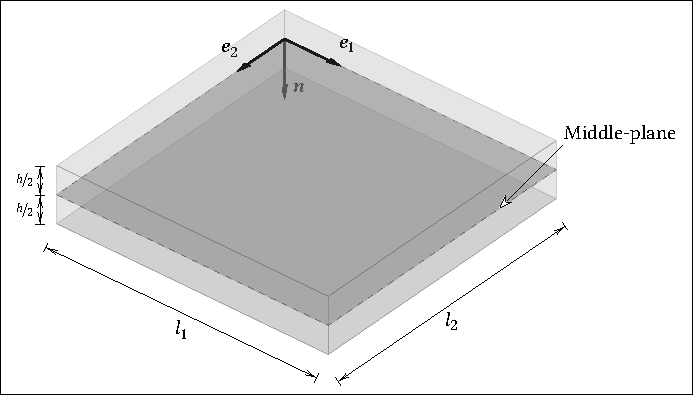
\includegraphics[scale=1]{typical_plate.pdf}
\caption{A typical plate and its middle-plane}\label{fig:generalplate}
\end{figure}

	\paragraph{Selecting a theory} Selecting the proper plate theory, among the classic ones, requires addressing two consideration~\autocite{Birman.2011}:
	\begin{enumerate}
		\item Thickness of the plate ($h$) and its transverse shear stiffness: thick plates with low transverse shear stiffness are best described by shear-deformable theories. The thinness of a plate is defined by empirical measures, e.g., a thickness less than one-tenth of its smallest dimension is considered thin $h<0.1\text{min}(l_1,l_2)$~\autocite{Altenbach.2008} or more restrictive values such as $h<0.05\text{min}(l_1,l_2)$~\autocite{Ugural.2010}. 
		\item Geometrical linearity or non-linearity of the problem: it is determined by the relative magnitude of deflection ($w$) to plate thickness. Namely, non-linearity is negligible for `small' deformations, i.e., deflections smaller than the empirical values of ($w<0.5h$)~\autocite{Birman.2011} or ($w<0.2h$)~\autocite{Altenbach.2008}. 
	\end{enumerate}
	In the absence of the shear strain components, deformation of the thin plate is dominated by bending. However, the effect of shear should be considered through some correction factors in special cases, e.g., plates with holes~\autocite{Timoshenko.1959}.

The adopted criterion of linearity assures the applicability of the small-deflection models in which the Green-Lagrange strain tensor reduces to the linearised strain measure because of the negligible quadratic slope terms. The other consequence of small deformations is that the middle-plane does not strain and becomes the neutral plane.

\paragraph{Plate categories} Note that the overlap of geometrical non-linearity and shear deformability is not common except for the case of sandwich panels with a very soft core. Therefore, based on the two aforementioned aspect, three categories of plates are recognised:
\begin{enumerate}
\item thin plates with small deformations,
\item thin plates with large deformations, and
\item thick plates.
\end{enumerate}









% ──────────────────────────────────────────────────────────────────────────────────────────────────
\subsection{Shear-Rigid Plate Theory}
The classic small-deformation thin plate theory is an extension of the Euler-Bernoulli beam theory. The theory ignores geometrical non-linearity and it is based on the Kirchhoff-Love hypotheses~\autocite{Reddy.2006}, which assume that the transverse normals\,\footnote{Transverse normals are the straight lines that are perpendicular to the middle-surface.} 
\begin{itemize}
\item remain straight after deformation,
\item are rigid, and
\item remain perpendicular to the middle-surface after deformation.
\end{itemize}
These assumptions have the following implications:
\begin{itemize}
\item Having `straight transverse normals after deformation' results in a linear distribution of strains through the cross-section. Thus, the middle-plane and the neutral plane coincide. In contrast, in the case of large deformations of a thin plate, the middle-plane is also strained. 
\item Due to the rigidity of the transverse normals, the thickness of the plate remains constant, i.e., no normal strains perpendicular to the neutral plane exists ($\varepsilon_{33}=0$). Consequently, the deflection of the plate becomes independent of the normal coordinate. Additionally, the normal transverse stress is usually ignored and does not enter the equilibrium equations since it is usually one order of magnitude smaller than transverse shear stresses ($\sigma_{33}\approx 0$). Thus, plane stress and constant thickness conditions are consequences of the current restriction.
\item `Transverse normals remaining perpendicular' indicates that shear deformability is neglected, i.e., the transverse shear strains ($\varepsilon_{13}$ and $\varepsilon_{23}$) are negligible. Note that although transverse shear strains are ignored, the internal transverse shear forces are obtained from the equilibrium conditions.
\end{itemize}
The Kirchhoff-Love assumptions form the shear-rigid plate theory, which is suitable for thin plates or plates with high transverse shear stiffness. 

% ──────────────────────────────────────────────────────────────────────────────────────────────────
\subsection{Shear-Deformable Plate Theory}
The shear deformable plate theory is an improvement to the shear-rigid plate theory by considering the shear strain deformations since the latter theory underestimates the deflections in thick plates. Also from another point of view, the theory is an extension of the Timoshenko beam theory to plates. 

The shear deformable theory is developed in different orders, which determine how the rotations of transverse normals are related to planar displacements. For instance, releasing the perpendicularity restriction of transverse normals results in the first-order shear deformable plate theory, i.e., additional rotations of the transverse normals due to shear strains are linearly related to each other. Releasing the straightness restriction of the transverse normals results in the third-order shear deformable theory, i.e., straight cross sections may become cubic curves after deformation~\autocite{Reddy.2006}.


\section{Laminate/Sandwich Theories}
	In terms of composite laminates and sandwiches, two main approaches exist:
	\begin{enumerate}
	\item The \textit{equivalent single-layer theories} (ESLTs)~\autocite{Altenbach.2010c} adopt the derived approach to transform the 3D problem into an equivalent 2D one. The assumptions are continuity of the displacements and/or strains through thickness. Two famous ESLTs are the classic laminate theory (CLT) (demands C\textsuperscript{1}-continuity) and first-order shear deformation theory (FSDT) (demands C\textsuperscript{0}-continuity); the former is used for thin laminates whereas the latter is used for thicker laminates and sandwiches.
	\item The \textit{layer-wise theories} (LWTs) require only C\textsuperscript{0}-continuity of through-thickness displacement but could be kinematically more accurate by incorporating layer-wise transverse shear effect into the displacement field~\autocite{Altenbach.2010c}. They could result in effortless FE implementations, see~\autocite{Javanbakht.2019b}.
	\end{enumerate}
	Among the ESLTs, the CLT is discussed in the sequel.

\paragraph{Assumptions of CLT} Classic laminate theory is merely the extension of thin plate theory to accommodate laminates. It is based upon the following assumption~\autocite{Herakovich.1998}:
    \begin{enumerate}
        \item perfect inter-layer bonding exists,
        \item each layer is homogeneous and can be orthotropic, transversely isotropic, or isotropic,
        \item each layer is in the plane stress state\,\footnote{In plane stress state, there exists a strain perpendicular to the plane of stress due to Poisson's effect, which will be ignored in the current context. Namely, no thickness change will be considered in CLT.}, and
        \item the laminate deforms according to shear-rigid theory.
    \end{enumerate}



\paragraph{Stress and Moment-Stress Resultants}	Consider the coordinate system in Fig.~\ref{fig:internal_force} that is established on the middle-plane of a plate (or equivalently a ply of a laminate). The basis vectors of $\base_1,\base_2$ and $\tena{n}$ are selected in a way that $\tena{n}$ is perpendicular to the middle plane; the respective coordinates are $X_1,X_2$ and $X_3$. Thereby, the Cauchy stress tensor is decomposed into	
	\begin{equation}
	\tenb{\sigma}=\sigma_{\alpha\beta}\base_\alpha\dyad\base_\beta+\sigma_{\alpha 3}\base_\alpha\dyad\tena{n}+\sigma_{3 \alpha}\tena{n}\dyad\base_\alpha+\sigma_{33}\tena{n}\dyad\tena{n},
	\end{equation}
	where the Greek indices vary from 1 to 2. 
\begin{figure}[!h]
\centering
\subfloat[Membrane and shear force resultants]{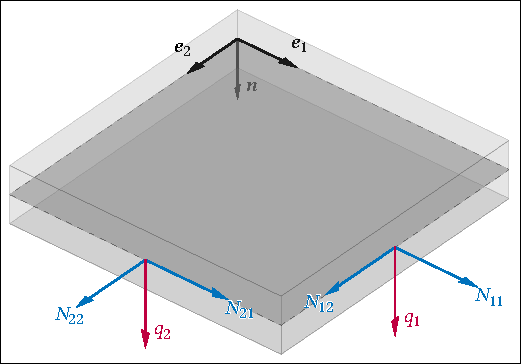
\includegraphics[scale=1]{plate_membrane_shear.pdf}}\\
\subfloat[Bending and twisting moment resultants]{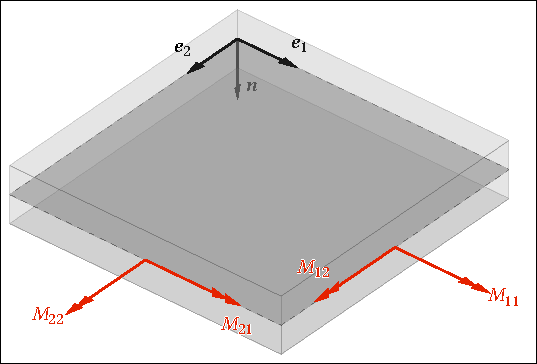
\includegraphics[scale=1]{plate_moment.pdf}}
\caption{Internal forces in a plate denoted at their positive direction}
\label{fig:internal_force}
\end{figure}%	
	If the first fundamental tensor of the surface ($\tenb{A}\equidef\tena{n}\dyad\tena{n}$)~\autocite{Eremeyev.2013} is used as a projection tensor, the 3D stress tensor could be readily projected onto the $1$-$2$ plane to form a non-symmetrical stress tensor:
	\begin{equation}
	\tenb{A}\scp\tenb{\sigma}=\sigma_{\alpha\beta}\base_\alpha\dyad\base_\beta+\sigma_{\alpha 3}\base_\alpha\dyad\tena{n},
	\end{equation}
	where $\tenb{A}\scp\tenb{\sigma}$ holds the membrane stress components $\sigma_{\alpha\beta}$ and transverse shear stress components $\sigma_{\alpha 3}$. Thereby, all the stress components on the surface with the normal of $\tena{n}$ are discarded. Now, the distribution of other stress components through thickness must by taken into account and then eliminated. To this end, the through-thickness integration operator is defined as
	\begin{equation}
	\inbrack{\Box}\equiv\thickint{\Box},
	\end{equation}
	where a structural thickness of $h$ is assumed for a plate with a normal along the 3-axis. Applying this operator to the non-symmetrical stress tensor results in
	\begin{equation}
	\inbrack{\tenb{A}\scp\tenb{\sigma}}=\tenb{N}+\tena{q}\dyad\tena{n},
	\end{equation}
	where $\tenb{N}\equiv \tenb{A}\Rayleigh\tenb{\sigma}=\inbrack{\sigma_{\alpha\beta}\base_\alpha\dyad\base_\beta}$ is the membrane stress resultant tensor and $\tena{q}=\inbrack{\sigma_{\alpha 3}\base_\alpha}$ is the transverse shear stress resultant vector. 
	
	Furthermore, the axial (bending/twisting) moment tensor, resulting from the membrane stresses, is defined as
	\begin{equation}
	\tenb{M}\equidef \inbrack{-X_3 \sigma_{\alpha\beta}\base_\alpha\dyad\base_\beta\cross\tena{n}},
	\end{equation}
	which could be replaced by its polar counterpart by removing the axial property of its second index
	\begin{equation}
	\tenb{L}\equidef \tenb{M}\cross \tena{n} = X_3 \sigma_{\alpha\beta}\base_\alpha\dyad\base_\beta,
	\end{equation}
	where $\tenb{L}$ is the polar (bending/twisting) moment tensor. 
	
	The calculated stress and moment resultants were for a single plate or ply; it can be extended to the case of a laminate structure. Namely, all the equations will be correct for each ply separately. In the CLT, the sum of these values will be used to obtain the equivalent single layer. In the following, the tensor notation will change to matrix Voigt notation, which is the common one for CLT. Namely, the stress and moment stress resultants become
	\begin{align}
		\col{N}&=\lfloor N_{11}\;N_{22}\;N_{12}\rfloor^\tran=\lfloor N_{1}\;N_{2}\;N_{6}\rfloor^\tran,\\
		\col{q}&=\lfloor q_{1}\;q_{2}\rfloor^\tran,\\
		\col{M}&=\lfloor M_{11}\;M_{22}\;M_{12}\rfloor^\tran=\lfloor M_{1}\;M_{2}\;M_{6}\rfloor^\tran,
	\end{align}
	in Voigt notation.

\paragraph{Kinematics} 	The strains of the middle-plane ($\{\mbfsansepsilon\}$) are related to the through-thickness strain field by
	\begin{equation}
	 \{\mbfsansvarepsilon(X_1,X_2,X_3)\}	= \{\mbfsansepsilon (X_1,X_2)\}+X_3\{\mbfsanskappa(X_1,X_2)\},
	\end{equation}
	 where $\symbf{\col{\mbfsanskappa}}=\lfloor \kappa_{11}\;\kappa_{22}\;\kappa_{12} \rfloor^\tran$ is the vector of bending/twisting curvature, $X_3\symbf{\col{\mbfsanskappa}}$ is the vector of flexural strains, and $\col{\mbfsansepsilon}$ is the vector of membrane (in-plane) strains. Note that since the curvature is constant through thickness (a consequence of the first assumption), the contribution of the flexural strain is linear with respect to the third coordinate. The membrane strains are also constant through thickness.


\paragraph{Resultants in laminates} For a laminate with $n$ arbitrarily-oriented plies, the overall thickness of the laminate is
\begin{equation}
	h=\sum_{k=1}^{n} h^{(k)},
\end{equation}
where $h^{(k)}$ is the thickness of the $k$-th ply from the middle-plane; namely:
\begin{equation}
	h^{(k)}=X_3^{(k)}-X_3^{(k-1)},\qquad\forall k\in\{1,2,\ldots,n\},
\end{equation}
where $X_3^{(k)}$ is the furthest distance of the $k$-th ply from the middle-plane along the normal $\tena{n}$.

The total in-plane stress resultant force vector $\col{N}$, total transverse shear resultants $\col{q}$ and the total moment-stress resultant vector $\col{M}$ of the laminate is
\begin{subequations}
\begin{align}
	\col{N}&= \sum_{k=1}^{n} \{{\symbfsf N}^{(k)}\},\\
	\col{q}&= \sum_{k=1}^{n} \{{\symbfsf q}^{(k)}\},\\
	\col{M}&= \sum_{k=1}^{n} \{{\symbfsf M}^{(k)}\},
\end{align}
\end{subequations}
	where $\{{\symbfsf N}^{(k)}\}$, $\{{\symbfsf q}^{(k)}\}$ and $\{{\symbfsf M}^{(k)}\}$ are the in-plane stress, transverse shear stress, and moment-stress resultant vector of the $k$-th ply, respectively. It can be shown that the transverse shear resultant does not couple with the other two resultants, and thus the interactions of the flexural and in-plane states read
\begin{equation}
	\left[
	\begin{array}{c}
		\col{N}\\\hline
		\col{M}
	\end{array}
	\right]
	=
	\left[
		\begin{array}{@{}c|c@{}}
			\mat{A}& \mat{B}\\\hline
			\mat{B}& \mat{D}\\
		\end{array}
	\right]
	\left[
	\begin{array}{c}
		\symbf{\col{\mbfitsansepsilon}}\\\hline
		\symbf{\col{\mbfitsanskappa}}
	\end{array}
	\right],
\end{equation}	
where $\mat{A},\mat{B}$, and $\mat{D}$ are the extensional, coupling, and bending stiffness sub-matrices, respectively. The transverse shear resultant is related to the shear strain vector $\col{\mbfitsansgamma^\text{\normalfont s}}$ by
\begin{equation}
	\col{q}=\symbf{\mat{A^\text{\normalfont s}}} \col{\mbfitsansgamma^\text{\normalfont s}},
\end{equation}
where $\symbf{\mat{A^\text{\normalfont s}}}$ is the transverse shear stiffness matrix. The contribution of each layer to the total stiffness matrices is
\begin{alignat}{3}
\mat{A}&=&                              \sum_{k=1}^{n}& \left[{\tilde{\symbfsf C}}^{(k)}\right] \left(X_3^{(k)}- X_3^{(k-1)}\right),\\
\mat{B}&=&                   \frac{1}{2}\sum_{k=1}^{n}& \left[{\tilde{\symbfsf C}}^{(k)}\right] \left( (X_3^{(k)})^2- (X_3^{(k-1)})^2\right),\\
\mat{D}&=&                   \frac{1}{3}\sum_{k=1}^{n}& \left[{\tilde{\symbfsf C}}^{(k)}\right] \left( (X_3^{(k)})^3- (X_3^{(k-1)})^3\right),\\
\symbf{\mat{A^\text{\normalfont s}}} &=&\sum_{k=1}^{n}& \left[{\symbfsf C}^{(k)}\right] \left(X_3^{(k)}- X_3^{(k-1)}\right),
\end{alignat}
where $\left[{\symbfsf C}^{(k)}\right]$ is the stiffness matrix of the $k$-th layer and $\left[{\tilde{\symbfsf C}}^{(k)}\right]$ is the reduced stiffness matrix of the $k$-th layer, see~\autocite{Altenbach.2010c,Herakovich.1998,Barbero.2017}.



%
%
%% ══════════════════════════════════════════════════════════════════════════════════════════════════
%\section{The Direct Approach}
%    In the following sections, a 3D continuum is reformulated as a 2D surface by means of the direct approach. Although no exact 2D~shell theory exists, a 2D~surface is a facilitative vehicle for mathematical formulation. Thus, the direct approach takes the 2D~surface as a primitive concept while denying it as a 3D~entity~\autocite{Libai.2005}. Aligned with this approach, simple shells are considered as 2D continua in which the interaction of the body sections is done via forces and moments~\autocite{Zhilin.1976}. 
%    
%    Herein, the so-called direct approach is used to obtain the theory for simple shells. This approach takes advantage of the fact that the directed deformable surfaces inherently have the same DoFs as those required in the shell theories. In the common shell theories of the Cauchy continua, translational DoFs are used along with some assumptions to obtain the kinematics of the problem whereas the directed surface theory has all the required kinematic quantities. Namely, all the ingredients of a shell theory, i.e., rotations and translations, are already incorporated in the directed surface effortlessly. Therefore, an assumption-free approach can be adopted.
%
%    Media with micro-structure deviate from the classical local theories and are represented using one of the 3M continua, i.e., micromorphic, microstretch, or micropolar continua with 9, 4, and 3 additional DoFs, respectively~\autocite{Eringen.1998}. The additional DoFs are assigned to each point by means of a triad of vectors---called \textit{directors}---which capture the microdeformations of the internal structure.
%
%    The most general micromorphic continuum uses deformable directors to incorporate point-wise shear, stretch, and rotations. In microstretch continuum microshearing is not possible but rotations and stretches are allowed. Finally, the micropolar continua assigns only rotations via rigid directors. Following this hierarchy, the classical Cauchy continuum is the one without any directors, i.e., it is not a directed medium. 
%    
%    Among the 3M~media, the micropolar continua have the required additional rotations, and thus it is the starting point of the direct approach. Due to the in-plane rigidity of shells, only two rotations out of the available three rotations are practically necessary. Namely, the rotations about the normal vector of the shell are neglected resulting in the so-called \textit{5-DoF theories}.
%    
%\subsection{Kinematics}
%In the 5-DoF Mindlin plate theory, three translations and two rotations are present. Zhilin \autocite*{Zhilin.1976} introduces the following DoFs: 
%\begin{alignat}{2}
%&\tena{u}   &&=u_i\base_i,\\
%&\tena{\psi}&&=\psi_\alpha\base_\alpha=-\varphi_2\base_1+\varphi_1\base_2,
%\end{alignat}
%whereas Pal'mov's \autocite*{Palmov.1982} alternative DoFs result in a better symmetry in the numerical solution:
%\begin{alignat}{3}
%&\tena{u}&&=\tena{v}+w\tena{n}&&\hspace*{2cm}\text{with}\,\tena{v}=v_\alpha\tena{e}_\alpha\;,\\
%&\tena{\varphi}&&=\varphi_\alpha\tena{e}_\alpha\;,&&
%\end{alignat}
%where $\tena{u}$ is the displacement vector, $\tena{v}$ is the in-plane displacement vector, $w\tena{n}$ is the deflection vector, and $\tena{\varphi}$ is the out-of-plane rotation vector.
%
%\subsection{Strain Measures}
%
%
%
%
%% ══════════════════════════════════════════════════════════════════════════════════════════════════
%\section{Formulation of The Equilibrium Equations}
%
%
%
%\subsection{General 3D Micropolar Continua}
%In micropolar media, linear momentum ($\tena{\symbfscr{l}}$) and angular momentum ($\tena{\symbfscr{m}}$) of a volumetric part of the whole body ($\Part\subseteq\Body$) are respectively defined as
%\begin{alignat}{1}
%\tena{\symbfscr{l}}&\equidef\iiint_{\Part}\rho\tena{v}\dif V\\
%\tena{\symbfscr{m}}&\equidef\iiint_{\Part}\big[(\tena{r}-\tena{r}_0)\cross\rho\tena{v}+j\tena{\omega}\big]\,\dif V,
%\end{alignat}
%where $\tena{v}$ is the velocity field, $\tena{r}$ is the position vector, $\tena{r}_0$ is the position vector with respect to an arbitrary reference point, $j$ is the moment of inertia of the microparticles, and $\tena{\omega}$ is the angular velocity field. Euler's first and second laws of motion state the balance law for the linear momentum and angular momentum of a dynamic body, respectively. Namely, for a body under external force, the rates of change of linear momentum and the angular momentum about a point are equal to the total force acting on the body and the total moment acting on the body about the same point, respectively. Consequently, in a body without any external stimuli, both linear and angular momentums are conserved. Euler's laws of motion for an oriented medium are
%\begin{alignat}{3}
%\tena{\symbfscr{p}}&\equidef{\dif \tena{\symbfscr{l}} \over \dif t}&&\equimust \iiint_{\Part}\rho\tena{b}\,\dif V                                       &&+\oiint_{\partial\Part}\tena{t}\,\dif A\\
%\tena{\symbfscr{c}}&\equidef{\dif \tena{\symbfscr{m}} \over \dif t}&&\equimust \iiint_{\Part}\big[(\tena{r}-\tena{r}_0)\cross\rho\tena{f}+\rho\tena{l}\big]\,\dif V&&+\oiint_{\partial\Part}\big[(\tena{r}-\tena{r}_0)\cross\tena{t}+\tena{\mu}\big]\,\dif A,
%\end{alignat}
%where $\rho$ is the mass density, $\tena{t}$ is the stress vector (contact force per unit area), $\tena{\mu}$ is the couple stress vector (contact couple per unit area), $\tena{b}$ is the body force vector (per unit mass), and $\tena{l}$ is the body couple vector (per unit mass). Applying the Gauss-Ostrogradsky theorem to these equations results in the local form of Euler's equations of motion:
%\begin{alignat}{3}
%\diver{\tenb{T}}  &+\rho \tena{b}&                 &=\rho{\dif \tena{v}\over\dif \tena{t}},\\
% \diver{\tenb{\mu}}&+\rho \tena{l}&\;+\,\gibbs{\tenb{T}}&=j{\dif\tena{\omega}\over\dif t}.
%\end{alignat}
%Note that only Euler's first law of motion (in either global or local forms) is identical for both Cauchy and oriented media. In 3D micropolar continua, Euler's equations of motion in the absence of inertia forces are described in the local form as
%\begin{alignat}{2}
%\label{eq:lm} \diver{\tenb{T}}  &+\rho \tena{b}&                 &=\tena{0},\\
%\label{eq:am} \diver{\tenb{\mu}}&+\rho \tena{l}&\;+\,\gibbs{\tenb{T}}&=\tena{0}.
%\end{alignat}
%% ──────────────────────────────────────────────────────────────────────────────────────────────────
%\subsection{Reduction to Planar Continua}
%Herein, a flat shell on the $1$-$2$ plane is formulated from a 3D continuum. The closed surface of the 3D body volume ($\Surface\equiv\partial\Volume$) is divided into two subsets: the kinematic boundary conditions are applied on the first one ($\Surface_u$) and the static boundary conditions are applied on the remaining part ($\Surface-\Surface_\text{u}=\Surface_\text{t}$):
%\begin{subequations}
%\begin{alignat}{3}
%&\Surface_\text{u}&:\quad&&                    \tena{u}&=\tena{u}_0,\\
%                       &&&&                    \tena{\varphi}&=\tena{\varphi}_0,\\
%&\Surface_\text{t}&:\quad&& \tena{n} \scp \tenb{T}     &=\tena{f}_0,\\
%&                 &      && \tena{n} \scp \tenb{\mu}   &=\tena{m}_0.
%\end{alignat}
%\end{subequations}

%% ══════════════════════════════════════════════════════════════════════════════════════════════════
%\section{Thermal Effects on a Single Mindlin Plate}
%The thermal effects are considered through the following assumptions:
%\begin{enumerate}
%\item Mindlin plate assumption forces a plain stress state for the plate, and therefore thermal thickness changes are ignored,
%\item material properties, e.g., elastic modulus, shear modulus, Poisson's ratio and the coefficient of thermal expansion, are temperature-independent, and thus the neutral surface coincides with the middle-plane of the plate~\autocite{Mansfield.1989},
%\item the effect of heat flux through the plate can be implicitly considered as through-thickness temperature change by adopting a smooth spatial thermal field ($T\equiv T(X_1,X_2,X_3)$); herein, the through-thickness temperature change is ignored ($T\equiv T(X_1,X_2)$),
%\item geometrically nonlinear terms are ignored in measuring the strains, and
%\item the plate is considered to be isotropic and homogeneous, i.e., $\alpha_1=\alpha_2=\alpha$ and $\alpha_{12}=0$, and thus no membrane shear deformation is induced in the plate due to the temperature field.
%\end{enumerate}
%
%% Considering a through-thickness temperature variation:
%% \begin{alignat}{8}
%% &\tenb{N}^\theta=2B\inangle{\alpha\Delta\theta}\tenb{P},\\
%% &\tenb{L}^\theta=2B\inangle{\alpha\Delta\theta X_3}\tenb{P}.
%% \end{alignat}
%% Herein, a uniform through-thickness temperature is assumed.
%%───────────────────────────────────────────────────────────────────────────────────────────────────
%\subsection{Kinematics}
%In the 5-DoF Mindlin plate theory, three translations and two rotations are present. Zhilin \autocite*{Zhilin.1976} introduces the following DoFs: 
%\begin{alignat}{2}
%&\tena{u}   &&=u_i\base_i,\\
%&\tena{\psi}&&=\psi_\alpha\base_\alpha=-\varphi_2\base_1+\varphi_1\base_2,
%\end{alignat}
%whereas Pal'mov's \autocite*{Palmov.1982} alternative DoFs result in a better symmetry in the numerical solution:
%\begin{alignat}{3}
%&\tena{u}&&=\tena{v}+w\tena{n}&&\hspace*{2cm}\text{with}\,\tena{v}=v_\alpha\tena{e}_\alpha\;,\\
%&\tena{\varphi}&&=\varphi_\alpha\tena{e}_\alpha\;,&&
%\end{alignat}
%where $\tena{u}$ is the displacement vector, $\tena{v}$ is the in-plane displacement vector, $w\tena{n}$ is the deflection vector, and $\tena{\varphi}$ is the out-of-plane rotation vector.
%
%The existing eigenstrains and eigenstresses in the material are additively decomposed to thermal ($\op^\muptheta$) and residual ($\op^0$) components. Therefore, considering the Duhamel-Neumann analogy, the total strain is
%\begin{equation}
%\tenb{E}^{\mupSigma}=\tenb{E}+\tenb{E}^\muptheta+\tenb{E}^0,\label{eq:eignestrain}
%\end{equation}
%where $\tenb{E}$ is the tensor of elastic strain. Note that the compatibility condition of the strains is enforced via
%\begin{equation}
%\tenb{E}^{\mupSigma}=\gradsym{\tena{u}}.\label{eq:compat}
%\end{equation}
%The strains can be decoupled in terms of membrane strains ($\tenb{G}$), curvature changes ($\tenb{K}$), and transverse shear strains ($\tenb{g}$) according to the first-order shear deformable plate theory:
%\begin{equation}
%\tenb{E}^{\mupSigma}=\tenb{G}^{\mupSigma}+X_3\tenb{K}^{\mupSigma}+{1\over 2}\tena{g}^{\mupSigma}\dyad\tena{n}.
%\end{equation}
%Thus, the compatibility condition Eq.~\eqref{eq:compat} can be rewritten in the form of
%\begin{alignat}{3}
%\tenb{G}^{\mupSigma}&=\gradsym{\tena{v}},\\
%\tenb{K}^{\mupSigma}&=\gradsym{\tena{\varphi}},\\
%\tenb{g}^{\mupSigma}&=\grad{w}+\tena{\varphi}.
%\end{alignat}
%Similar to Eq.~\eqref{eq:eignestrain}, the decoupled strain measures can be expressed as
%\begin{alignat}{5}
%\tenb{G}^{\mupSigma}&=\tenb{G}&&+\tenb{G}^\muptheta&&+&\tenb{G}^0,\\
%\tenb{K}^{\mupSigma}&=\tenb{K}&&+\nulla            &&+&\tenb{K}^0,\\
%\tena{g}^{\mupSigma}&=\tena{g}&&+\nulla            &&+&\tena{g}^0,
%\end{alignat}
%where the decoupled thermal strains are
%\begin{alignat}{5}
%\tenb{G}^{\muptheta}&=\alpha\Delta\theta\tenb{P},\\
%\tenb{K}^{\muptheta}&=\nulla,\\%{\alpha\Delta\theta \over X_3}\tenb{P}={1\over X_3}\tenb{G}^{\muptheta},\\
%\tena{g}^{\muptheta}&=\nulla.
%\end{alignat}
%
%
%%───────────────────────────────────────────────────────────────────────────────────────────────────
%\subsection{Constitutive Law}
%Based on the Duhamel-Neumann analogy, the total stress is
%\begin{equation}
%\tenb{T}^{\mupSigma}=\tenb{T}-\tenb{T}^\muptheta-\tenb{T}^0,\label{eq:strs}
%\end{equation}
%where $\tenb{T}$ is the elastic stress tensor. However, the thermal eigenstresses will be present only in the case of incompatible thermal eigenstrains, e.g., in non-uniform temperature changes through thickness, when the material is anisotropic, or in the presence of constraints. In the case of non-zero uniform thermal strains, the respective thermal stresses are obtained from
%\begin{equation}
%\tenb{T}^{\muptheta}\!=3K\tenb{E}^\muptheta,
%\end{equation}
%where $K={3(1-2\nu) \over Y}$ is the bulk modulus. Herein, it is assumed that a homogeneous thermal field is applied, and thus $\tenb{T}^\muptheta=\tenb{0}$ and $\tenb{E}^\muptheta\neq\tenb{0}$ gives
%\begin{equation}
%\tenb{T}^{\mupSigma}=\tenb{T}-\tenb{T}^0.\label{eq:eigenstress}
%\end{equation}
%Consequently, the thermal effect is considered only via the thermal eigenstrains without any thermal eigenstresses. On the other hand, both of the residual (initial) eigenstresses and eigenstrains are taken into account, cf.~Eqs.~\eqref{eq:eignestrain} and \eqref{eq:strs}.\\
%Applying the over-thickness integration operator to Eq.~\eqref{eq:eigenstress} results in 
%\begin{equation}
%N_{\alpha\beta}=\inangle{T_{\alpha\beta}}\rightarrow \tenb{N}^{\mupSigma}=\tenb{N}-\tenb{N}^0,
%\end{equation}
%where $\tenb{N}$ is the membrane force tensor. Multiplying this equation by $X_3$ and applying the same operator results in
%\begin{equation}
%\tenb{L}^{\mupSigma}=\tenb{L}-\tenb{L}^0,
%\end{equation}
%where $\tenb{L}$ denotes the polar (bending/twisting) moment tensor.\\
%The 3D constitutive equation is expressed as~\autocite{Mura.1982}:
%\begin{equation}
%\tenb{T}^{\mupSigma}=\tend{C}\dscp \tenb{E},
%\end{equation}
%which is combined with Eqs.~\eqref{eq:eigenstress} and \eqref{eq:eignestrain} resulting in the generalised form of Duhamel-Neumann law:
%\begin{equation}
%\tenb{T}=\tend{C}\dscp(\tenb{E}^\mupSigma-\tenb{E}^\muptheta-\tenb{E}^0)+\tenb{T}^0.
%\end{equation}
%%───────────────────────────────────────────────────────────────────────────────────────────────────
%\subsection{Balance Equations}
%
%
%
%
%
%
%Since eigenstresses are already in-balance internally, the local form of the principle of balance of linear momentum (Cauchy's equation) can be readily stated in terms of elastic stresses:
%\begin{equation}
%\diver{\tenb{T}}+\rho \tena{b}=\tena{0}.
%\end{equation}
%The external distributed force vector ($\tena{f}$) is composed of two components
%\begin{alignat}{4}
%&\tena{f}=\tena{s}+\tena{q},&\qquad\text{with}\quad& \tena{s}=-s_\alpha\base_\alpha,\quad \tena{q}=q\tena{n},
%\end{alignat}
%where $\tena{s}$ is the tangential distributed external force vector, and $\tena{q}$ is the normally distributed force vector.
%
%
%In the absence of inertia forces, the balance of linear and angular momentum for micropolar media are stated as
%\begin{alignat}{3}
%\div{a}
%\end{alignat}
%
%
%
%
%
%
%
%
%
%
%
%
%
%
%
%
%
%
%%───────────────────────────────────────────────────────────────────────────────────────────────────
%\subsection{Decoupled Kinetic Measures}
%Analogous to Eq.~\eqref{eq:eigenstress}, through-thickness integration of stress tensor results in
%\begin{subequations}
%\begin{alignat}{4}
%&\tenb{N}^{\mupSigma}&&=\tenb{N}&-&\tenb{N}^\muptheta&-&\tenb{N}^0,\\\label{eq:membrane}
%&\tenb{L}^{\mupSigma}&&=\tenb{L}&-&\tenb{L}^\muptheta&-&\tenb{L}^0,\\
%&\tena{q}^{\mupSigma}&&=\tena{q}&-&\nulla            &-&\tena{q}^0,
%\end{alignat}
%\end{subequations}
%where $\tenb{N}$ is the membrane stress resultant tensor, $\tenb{L}$ is the moments resultant  tensor, and $\tena{q}$ is the transverse shear stress resultant vector. The total membrane stress resultant is obtained by over-thickness integration of the total stress tensor:
%\begin{equation}
%\tenb{N}^{\mupSigma}=\inangle{\tena{P}\scp\tenb{T}\scp\tenb{P}},
%\end{equation}
%and results in
%\begin{align}
%\tenb{N}^{\mupSigma}=\tend{A}\dscp\tenb{G}&&\text{with}\;\tend{A}=2h\left[(B-G)\tend{P}^\vol+G\tend{P}^\sym\right].\label{eq:membranetotal}
%\end{align}
%The thermal stress resultant is obtained from
%\begin{equation}
%\tenb{N}^\muptheta=2Bh\tenb{G}^\muptheta\qquad\text{with}\quad\tenb{G}^\muptheta=\alpha\mupDelta\theta\tenb{P}.\label{eq:membranethermal}
%\end{equation}
%Thus, combining Eqs.~\eqref{eq:membrane}, \eqref{eq:membranethermal}, and \eqref{eq:membranetotal} results in the elastic components of the membrane stress resultant:
%\begin{equation}
%\tenb{N}=\tend{A}\dscp\tenb{G}+2Bh\tenb{G}^\muptheta+\tenb{N}^0.
%\end{equation}
%The total moment resultant is obtained by 
%\begin{equation}
%\tenb{L}^{\mupSigma}=\inangle{\tena{P}\scp\tenb{T}\scp\tenb{P}X_3},\label{eq:momentres}
%\end{equation}
%and results in
%\begin{align}
%\tenb{L}^{\mupSigma}=\tend{D}\dscp\tenb{K}&&\text{with}\;\tend{D}={h^3\over 6}\left[(B-G)\tend{P}^\vol +G\tend{P}^\sym\right].\label{eq:momentrestot}
%\end{align}
%The thermal moment resultant is obtained from
%\begin{align}
%\tenb{L}^\muptheta={Bh^2\over 2}\tenb{G}^\muptheta&&\text{with}\;\tenb{G}^\muptheta=\alpha\mupDelta\theta\tenb{P}.\label{eq:momentthermal}
%\end{align}
%Combining the Eqs.~\eqref{eq:momentres}, \eqref{eq:momentrestot} and \eqref{eq:momentthermal}, the elastic components of the moments resultant tensor are obtained:
%\begin{align}
%\tenb{L}=\tend{D}\dscp\tenb{K}+{Bh^2\over 2}\tenb{G}^\muptheta+\tenb{L}^0.
%\end{align}
%% ──────────────────────────────────────────────────────────────────────────────────────────────────





%---------------------------------------------------------------------------------------------------
\section{Anisotropic Failure Criteria} %TODO double check everything
	\paragraph{General mathematical form} A general failure criterion for anisotropic materials can take the following form~\autocite{Goldenblat.1966}:
	\begin{equation}\label{eq:strength_aniso}
		f\equidef \sum_{k=1}^{n}
		(\tenb{\sigma}^\tenpow{k}\odot\tenn{S}{2k})^{\alpha_k} \le 1,\qquad\qquad \alpha_k \in \Real,		
%		(\tenb{\sigma}\dscp\tenb{S})^\alpha + (\tenb{\sigma}^\tenpow{1}\contract\tend{S})^\beta +
%		(\tenb{\sigma}^\tenpow{2}\contract\tenn{S}{6})^\gamma + \ldots\le 1,\qquad\qquad \alpha, \beta, \gamma, ... \in \Real,
	\end{equation}
	where Cauchy stress tensor ($\tenb{\sigma}$), and strength tensors ($\ten{S}$) are related via the scalars ($\alpha_k$). The strength tensor is the stress tensor that is obtained upon the failure of material (the ultimate stress tensor)~\autocite{Malmeister.1969}. Strength tensors are elements of the strength/failure surface. For instance, a second-order strength tensor ($\tenb{S}\in\symset$) is geometrically represented by a surface in the six-dimensional space. Initially, some points on a failure surface are obtained via experimentations, and then by statistical analysis, a surface is obtained for a specific confidence level~\autocite{Malmeister.1969}. By choosing the appropriate scalars and the order of tensors, any failure surface can be represented mathematically by the calibration of Eq.~\eqref{eq:strength_aniso}; this is the so-called \textit{tensor method}. Some general examples are presented in the sequel.
	
	\paragraph{Tsai-Hill criterion} The extension of the Huber-Mises-Hencky criterion in isotropic materials to the orthotropic ones was carried out by Hill~\autocite{Hill.1998}. Later, the so-called Tsai-Hill Criterion is presented~\parencite{Azzi.1966}:
	\begin{equation}
		f_\text{Tsi-Hill}\equidef \left(\frac{\sigma_{11}}{S_{11}}\right)^2 + \left(\frac{\sigma_{22}}{S_{22}}\right)^2 + \left(\frac{\sigma_{12}}{S_{12}}\right)^2 - \frac{\sigma_{11}\sigma_{22}}{(S_{11})^2} \le 1,
	\end{equation}
	which is obtained by the quadratic terms of Eq.~\eqref{eq:strength_aniso}. Unlike the maximum stress criterion, no specific failure mode could be identified by this criterion.
	
	
	\paragraph{Tsai-Wu criterion} The Tsai-Wu criterion~\autocite{Tsai.1971} is a special case for which the linear and quadratic terms are used~($\alpha_1=\alpha_2=1$), i.e., the linear combination of first and second order tensors:
	\begin{equation}
		f_\text{Tsi-Wu}\equidef \tenb{\sigma}\dscp\tenb{S} + (\tenb{\sigma}\dyad\tenb{\sigma})\dscp\dscp\tenn{S}{4} =\tenb{\sigma}\dscp\tenb{S} + \tenb{\sigma}\dscp\tend{S}\dscp\tenb{\sigma}^\tran.
	\end{equation}	 



	
	\paragraph{Maximum stress criterion} In this criterion, the three axial, transverse and shear failure modes of fibre-reinforced composites are decoupled:
	\begin{alignat}{2}
		\sigma_{11} \ge S_{11},\\
		\sigma_{22} \ge S_{22},\\
		\sigma_{12} \ge S_{12}.
	\end{alignat}
	By using the maximum stress criterion in the off-axis loading of a unidirectional composite, the loading angle determines the strength and failure mode, see Fig.~\ref{fig:max_stress_crit}.
\begin{figure}[!h]
\centering
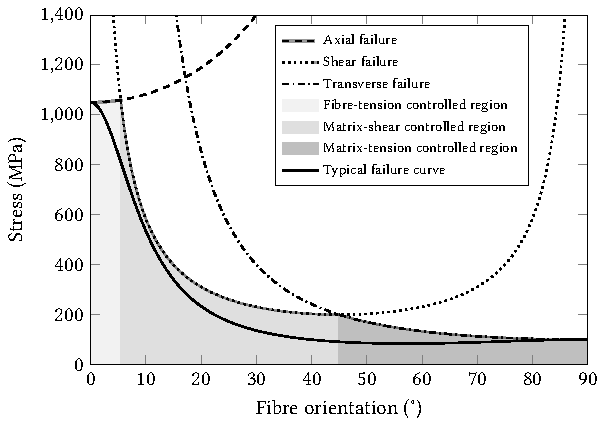
\includegraphics[scale=1]{lit_max_stress.pdf}
\caption{Dominant regions of various failure modes in a fibre-reinforced composite material due to uncoupled nature of the maximum stress criterion}\label{fig:max_stress_crit}
\end{figure}


	\paragraph{Cowin's failure criterion} 	A scalar-valued function of Cauchy stress tensor ($\tenb{\sigma}$), orientation tensor ($\tenb{H}$) and fibre volume fraction ($\zeta_\text{f}$) is assumed~\autocite{Cowin.1986}:
		\begin{equation}
			f\equiv f(\tenb{\sigma}, \tenb{H}, \zeta_\text{f}).
		\end{equation}
		Since the anisotropy of the continuum is incorporated by means of the orientation tensor, $f$ must succumb to every symmetry, i.e., it must satisfy the isotropy condition:
		\begin{equation}
			f(\tenb{\sigma}, \tenb{H}, \zeta_\text{f})\equimust f(\tenb{Q}\Rayleigh\tenb{\sigma}, \tenb{Q}\Rayleigh\tenb{H}, \zeta_\text{f}),
		\end{equation}
		where $\tenb{Q}$ is the orthogonal rotation tensor. Alternative to satisfying this equation, a form-invariant anstaz could be considered by including all the invariants of the parameters in the function~\autocite{Boehler.1987}:
		\begin{equation}
			f\equiv f\big(
			\tr{\tenb{\sigma}},\tr{\tenb{\sigma}^2},\tr{\tenb{\sigma}^3},
			\tr{\tenb{H}},\tr{\tenb{H}^2},\tr{\tenb{H}^3},
			\tr{(\tenb{\sigma}\scp\tenb{H})},\tr{(\tenb{\sigma}\scp\tenb{H}^2)},\tr{(\tenb{\sigma}^2\scp\tenb{H})},\tr{(\tenb{\sigma}^2\scp\tenb{H}^2)},\zeta_\text{f}\big).
		\end{equation}
		where $\tr{(\op)}\equidef\tenb{I}\dscp\op$ indicates the trace operator. The final result is a form of Eq.~\eqref{eq:strength_aniso} that only incorporates the linear and quadratic terms:
	\begin{equation}
		f_\text{Cowin}\equidef \tenb{\sigma}\dscp\tenb{S} + (\tenb{\sigma}\dyad\tenb{\sigma})\dscp\dscp\tend{S},
	\end{equation}	
	where the strength tensors are given as
	\begin{equation}
		\tenb{S} =\;g_1\unitb+g_2\tenb{H}+g_3\tenb{H}\scp\tenb{H},
	\end{equation}
	and
	\begin{alignat}{5}
	\nonumber 	\tend{S} =\;& \alpha_1 \unitd^\vol 
					+\alpha_2 (\tenb{H}\dyad\unitb)^\sym 
					+\alpha_3 (\tenb{H}\scp\tenb{H}\dyad\unitb)^\sym
					+\alpha_4 (\tenb{H}\dyad\tenb{H})\\\nonumber
	    			&+\alpha_5 (\tenb{H}\scp\tenb{H}\dyad\tenb{H})^\sym 
					+\alpha_6 (\tenb{H}\scp\tenb{H}\dyad\tenb{H}\scp\tenb{H})^\sym 
					+\alpha_7 \unitd^\sym\\
					&+\alpha_8 \big[(\tenb{H}\dyadu\unitb)^\sym + (\unitb\dyadu\tenb{H})^\sym\big]6
					+\alpha_9 \big[(\tenb{H}\scp\tenb{H}\dyadu\unitb)^\sym + (\unitb\dyadu\tenb{H}\scp\tenb{H})^\sym\big].
	\end{alignat}
	Note that this model requires nine parameters:
	\begin{alignat}{5}
		\alpha_i\equiv \alpha_i(\tr{\tenb{H}},\tr{\tenb{H}^2},\tr{\tenb{H}^3},\zeta_\text{f}),\qquad\qquad\forall i\in\{1,...,9\}.
	\end{alignat}		













\section{Micro-Mechanical Models}
	In this section, a background on obtaining the properties of particulate suspensions is provided. Then, the relation of such composite systems to solid-solid composites is discussed. In this regard, the classic Halpin-Tsai and Nielson models are reviewed.

\subsection{Hill Bounds \& Rule of Mixture} 
	As mentioned earlier, Cowin's formulation is used along with spectral analysis to detect the special cases. Moreover, the Hill bounds are used in developing the semi-analytical formulation of the effective properties for NFRCs. In the bounding methods of MFA, the volume averaging of an arbitrary field ($\tend{T}$) over the $\Omega$ domain is defined as
	\begin{equation}
	\avevol{\tend{T}} \equidef \int_{\Omega}\tend{T}(\tena{x})\dif\Omega,
	\end{equation}
	where $\tena{x}$ is the position vector. In a biphasic material, the domain consists of fibre (f) and matrix (m) volumes, i.e., $\Omega_\text{f} \cup \Omega_\text{m}=\Omega$ and $\Omega_\text{f} \cap \Omega_\text{m}=\varnothing$. To set up the micro-mechanical formulation for a multi-phase continuum, the micro-constitutive relation between the stress and strain of the $p$ phase is
	\begin{alignat}{2}
	\tenb{\sigma}^\text{(p)} &= \tend{C}^\text{(p)}\dscp\tenb{\varepsilon}^\text{(p)},\qquad\qquad\forall\text{p}\in\{\text{f},\text{m}\},
	\end{alignat}
	where $ \tend{C}^\text{(p)}$ is the elastic stiffness of the `p' phase. The averaged macro-constitutive relation for the homogenised medium is
	\begin{alignat}{2}
		\avevol{\tenb{\sigma}} &= \tend{C}_\text{eff}\dscp\avevol{\tenb{\varepsilon}},
	\end{alignat}
	where $\tend{C}_\text{eff}$ is the effective elastic stiffness of the multi-phase medium. The average stress and average strain of the medium are $\avevol{\tenb{\varepsilon}}=\sum\zeta^{(p)}\tenb{\varepsilon}^{(p)}$ and $\avevol{\tenb{\sigma}}	=\sum\zeta^{(p)}\tenb{\sigma}^{(p)}$ where $\zeta^{(p)}=\sfrac{\Omega_\text{p}}{\Omega}$ is the volume fraction of the `p' phase. In the next step, localisation tensors~\autocite{Hill.1963} are used to relate the overall averaged properties to the phase-averaged ones:
	\begin{alignat}{2}
	\forall\text{p}\in\{\text{f},\text{m}\}:\left\{
	\begin{array}{rl}
		\avevol{\tenb{\varepsilon}}^\text{(p)} &= \tend{A}^\text{(p)}\dscp\avevol{\tenb{\varepsilon}},\\[0.2cm]
		\avevol{\tenb{\sigma}}^\text{(p)} 	&= \tend{B}^\text{(p)}\dscp\avevol{\tenb{\sigma}}.
	\end{array}\right.,
	\end{alignat}
	where $\tend{A}$ and $\tend{B}$ are strain and stress concentration tensors, respectively.
	and obtain the effective elastic tensor
	\begin{equation}
	\tend{C}_\text{eff}=\sum_\text{(p)}\zeta^\text{(p)} \tend{A}^\text{(p)}\dscp\tend{C}^\text{(p)}.
	\end{equation}
	Adopting Voigt's assumption~\autocite{Voigt.1889} demands $ \avevol{\tenb{\varepsilon}^\text{(f)}}\equimust\avevol{\tenb{\varepsilon}^\text{(m)}}\equimust\avevol{\tenb{\varepsilon}}$ that results in the equality $\sum_\text{(p)}\zeta^{(p)}\tend{A}^\text{(p)}=\unitd^\sym$. Finally, the general form of rule of mixture for a bi-phasic medium is obtained
	\begin{equation}
	\tend{C}_\text{eff}=\sum_\text{(p)}\zeta^\text{(p)}\tend{C}^\text{(p)}.
	\end{equation}
	Adopting Reuss' assumption~\autocite{Reuss.1929} demands $ \avevol{\tenb{\sigma}^\text{(f)}}\equimust\avevol{\tenb{\sigma}^\text{(m)}}\equimust\avevol{\tenb{\sigma}}$ that results in the equality  $\sum_\text{(p)}\zeta^{(p)}\tend{B}^\text{(p)}=\unitd^\sym$. The general form of the inverse rule of mixture for a bi-phasic mediums is obtained
	\begin{equation}
	\tend{C}^\inv_\text{eff}=\sum_\text{(p)}\zeta^\text{(p)}\left(\tend{C}^\text{(p)}\right)^\inv.
	\end{equation}	
	
	 Finally, the Hill bound is obtained~\parencite{Bohm.2004}:
	\begin{equation}
		\Big[\sum_\text{(p)}\zeta^\text{(p)}(\tend{C}^\text{(p)})^\inv\Big]^\inv \le\tend{C}_\text{eff}\le\sum_\text{(p)}\zeta^\text{(p)}\tend{C}^\text{(p)},
	\end{equation}
	where $(\tend{C}^\text{(p)})^\inv$ is the compliance tensor of the phase `p'.

\paragraph{Rule of mixture} Expanding Hill's bound to their components results in the rule of mixture (RoM) and the inverse rule of mixture (IRoM):
	\begin{subequations}
	\begin{alignat}{2}
		E_\parallel 		=& \zeta_\text{f}E_\text{f}          &&+\zeta_\text{m}E_\text{m},\\
		\frac{1}{E_\perp}	=& \frac{\zeta_\text{f}}{E_\text{f}} &&+ \frac{\zeta_\text{m}}{E_\text{m}},
	\end{alignat}
	\end{subequations}
	where $\zeta$ is the volume fraction and $E$ is the elastic modulus. The subscripts `$\text{f}$' and `$\text{m}$' are used to denote the properties related to the fibres and the matrix, respectively. The elastic moduli $E_\parallel$ and $E_\perp$ are estimates in the longitudinal and transverse directions, respectively. Either formulation does not provide adequate meso-structural information regarding the composite material, and thus additional correction factors are applied to compensate this to some extent. The result is the so-called enhanced rule of mixture (En-RoM)~\autocite{Summerscales.2019}. The multiplication of the correction factors is regarded as an \textit{efficiency parameter} adjusting the contribution of fibres, see Chapters~\ref{chap:p6} and~\ref{chap:p7} for this extension.
	
\subsection{Viscosity Theory and Composite Systems}
	Viscosity is defined as the ratio of the shear stress $\tau$ to a fixed strain rate $\dot{\gamma}$---the stress is required to move a solution with a constant strain rate:
	\begin{equation}
		\eta \equidef \frac{\tau}{\dot{\gamma}(\tau)}.\label{eq:vis}
	\end{equation}
	In Newtonian fluids, viscosity does not depend on the shear rate. 
	
	In polymers, the viscosity can be used to estimate the molecular weight. Furthermore, one could calculate the effect of dissolving a solute on the viscosity of the solvent. To capture this effect, various measures of viscosity are introduced such as 
	\begin{subequations}
	\begin{alignat}{2}
		&\text{relative viscosity}\qquad& \eta_\text{r}  &\equidef \frac{\eta}{\eta_0}, \\
		&\text{specific viscosity}\qquad& \eta_\text{sp} &\equidef \frac{\eta-\eta_0}{\eta_0}, \\
		&\text{inherent viscosity}\qquad& \eta_\text{i}  &\equidef \frac{\ln\eta_\text{r}}{c}, \\
		&\text{intrinsic viscosity}\qquad& \left[\eta\right]  &\equidef \lim\limits_{c\rightarrow 0} \frac{\eta_\text{sp}}{c},
	\end{alignat}
	\end{subequations}
	where $\eta_0$ is the viscosity of the solution without the solute, $\eta$ is the viscosity of the solution with the $c$ the concentration of the solute. Relative viscosity and specific viscosity represent the change in the viscosity after dissolution in terms of final value and the change in the value, respectively. Inherent viscosity quantifies the sensitivity of the solution viscosity to change in the concentration of the solute. Intrinsic viscosity does a similar job but removes the dependency of inherent viscosity to concentration by taking a limit value. Namely, the definition of intrinsic viscosity can be set up by taking a limit value of the inherent viscosity and considering the fact that specific viscosity becomes very small at the limit:
	\begin{equation}\label{eq:spsv}
		\left[\eta\right] 
		\equidef  \lim\limits_{c\rightarrow 0} \ln \eta_\text{i}
		= \lim\limits_{c\rightarrow 0} \frac{\ln \eta_\text{r}}{c} 
		= \lim\limits_{c\rightarrow 0} \frac{\ln(1+\eta_\text{sp})}{c} 
		\approx \lim\limits_{c\rightarrow 0} \frac{\eta_\text{sp}}{c},
	\end{equation}
	in which Taylor's expansion is utilised and higher order terms are neglected. Namely, inherent and intrinsic viscosities have the same value as the concentration approaches zero. The result is a dimensionless material property which is independent of the concentration.
	Since intrinsic viscosity only depends on the molecular weight, it is the perfect tool for investigating the he effect of a solute in the viscosity of the solvent.
	
	Calculation of the intrinsic viscosity is done by calculating the specific viscosity for different concentrations and extrapolating the result to zero concentration. However, in an ideal solution\footnote{In an ideal gas, the interaction between molecules/atoms are negligible whereas in a liquid inter-molecular forces cannot be ignored. Thus, in an ideal liquid, the average inter-molecular interaction is assumed to be the same everywhere.}, the specific viscosity does not depend on concentration and taking a limit value is trivial\footnote{In ideal solutions, the inherent viscosity is obviously not equal to specific viscosity. Although specific viscosity is independent of concentration in ideal solutions, inherent viscosity will still depend on the concentration.}. In such cases, Eq.~\eqref{eq:spsv} reduces to
	\begin{equation}
		\left[\eta\right] = \frac{\eta_\text{sp}}{c},
	\end{equation}	
	and by rearranging, Einstein's equation to calculate the viscosity of a dilute suspension of rigid spherical particles is obtained:
	\begin{equation}
		\eta_\text{sol} = \eta_{\text{l}}(1+\left[\eta\right]c).\label{eq:ein}
	\end{equation}
	The theory of the viscosity of suspensions is extended to the theory of composite systems for obtaining the moduli of those systems. Similarities stem from the flow of suspensions during the manufacturing of composite materials~\autocite{Nielsen.1994}. Therefore, Eq.~\eqref{eq:ein} is restated for a composite system of particles and matrix:
	\begin{equation}
		\eta_\text{c} = \eta_{\text{m}}(1+k_\text{E}\zeta_\text{p, max}),
	\end{equation}	
	where $\eta_\text{c}$ is the viscosity of composite, $\eta_\text{m}$ is the viscosity of matrix, $\zeta_\text{p, max}$ is the maximum volume fraction possible for particles, and the intrinsic viscosity if relabelled to the so-called generalised Einstein's coefficient $k_\text{E}=2.5$.
	
	The maximum volume fraction for particles or the maximum packing fraction\footnote{This concept resembles the atomic packing factor of atoms in crystals, and thus quantifies how closely the particles can be packed.} is defined as
	\begin{equation}
		\zeta_\text{p, max}=\frac{V_\text{p, true}}{V_\text{p, apparent}},
	\end{equation}
	which is the ratio of the true volume of the particles ($V_\text{p, true}$) to the apparent volume ($V_\text{p, apparent}$). Since voids always exist between particles, the apparent volume is higher that the true volume, i.e., $\zeta_\text{p, max}<1$. For instance, cubic and hexagonal packing result in the maximum packing fractions of 0.524 and 0.78, respectively (see Table~\ref{table:apf}).

	\begin{table}[!h]
	\centering
	\caption{Maximum packing fractions. Adapted from~\autocite{Nielsen.1994}}\label{table:apf}
	\begin{tabular}{p{0.12\textwidth}p{0.6\textwidth}p{0.175\textwidth}}
	\toprule
	\bfs{Inclusion}	&	\bfs{Arrangement}	&	$\zeta_\text{p, max}$ \bfs{or} $\zeta_\text{f, max}$\\
	\toprule
	Spheres	
		& Hexagonal close packing, face-centred cubic packing	& 0.7405\\
		& Body-centred cubic									& 0.60\\
		& Simple cubic											& 0.5236\\
		& Random close packing, non-agglomerated				& 0.632\\
		& Random loose packing, non-agglomerated				& 0.601\\
		& Random close packing, agglomerated					& 0.37\\\midrule
	Fibres
		& Parallel hexagonal packing							& 0.907\\
		& Parallel random packing								& 0.85\\
		& Random orientation									& 0.52\\	
	\bottomrule
	\end{tabular}
	\end{table}
	
	Following the approach of moving from viscous solutions to composite solids, the rate of shear in Eq.~\eqref{eq:vis} is replaced by shear strain. Thus, for systems with incompressible matrices ($\nu=0.5$) like an elastomer that is filled with rigid particles, the shear moduli is theoretically related to viscosity values:
	\begin{equation}
		\frac{\eta_\text{c}}{\eta_\text{m}}=	\frac{G_\text{c}}{G_\text{m}},
	\end{equation}
	where $\eta_\text{c}$ and $\eta_\text{m}$ are the viscosity of the composite and matrix, and $G_\text{c}$ and $G_\text{m}$ are the shear modulus of the composite and matrix, respectively. Fundamentally, if a theory for viscosity of a multiple phase system exists, the same theory can be use to approximate the shear moduli~\autocite{Nielsen.1994}.
	

\subsection{The Halpin-Tsai \& Lewis-Nielsen Models}
    In order to approximate the elastic properties of composites, Halpin-Tsai generalised Kerner's approach~\autocite{Kerner.1956} that resulted in the following semi-empirical formulation~\autocite{Halpin.1976}:
    \begin{equation}
        \frac{M_\text{c}}{M_\text{m}}=\frac{1+AB\zeta_\text{f}}{1-B \zeta_\text{f}},\label{eq:HT}
    \end{equation}
    where $M_\text{c}$ is a modulus of the composite, $M_\text{m}$ is the corresponding modulus of the matrix, and $\zeta_\text{f}$ is the volume fraction of fibres. In the classic Halpin-Tsai, the RoM is used to calculate the axial modulus whereas the shear, transverse, or bulk moduli are calculated from Eq.~\eqref{eq:HT}. The parameter $A$ is related to the generalised Einstein's coefficient (intrinsic viscosity) by
   	\begin{equation}
   		A=k_\text{E}-1,
   	\end{equation}
   	and thus for rigid spheres $A$ is equal to 1.5 and for long aligned fibres it goes towards infinity. Parameter $B$ considers the relative moduli of the inclusions and matrix:
    \begin{equation}
       	B=\frac{\frac{M_\text{f}}{M_\text{m}}-1 }{\frac{M_\text{f}}{M_\text{m}}+A}.
    \end{equation}
    For high relative stiffness fibres, $B$ takes a unit value. 
    
    In order to consider the maximum packing factor of the inclusions~$V_\text{f,max}$, a further generalisation is applied by introducing the $\psi$ parameter that results in the Lewis-Nielson model~\autocite{Nielsen.1970}:
    \begin{equation}
        \frac{M_\text{c}}{M_\text{m}}=\frac{1+AB\zeta_\text{f}}{1-B\psi \zeta_\text{f}},
    \end{equation}
	where $M_\text{c}$ represents a modulus for the composite, e.g., axial, transverse, shear or bulk moduli, $M_\text{m}$ is the respective modulus of the matrix, and $\zeta_\text{f}$ is the volume fraction of fibres. One could see that substituting $\psi=1$ in the current model revives the classic Halpin-Tsai model. The $A$ and $B$ parameters are common between the two models: parameter~$B$ takes into account the property contrast between the fibre and matrix phases while the $A$~parameter considers the geometry of the inclusions (particles or fibres), packing arrangement, and loading condition~\autocite{Nielsen.1994}. For a known elastic modulus, its value can be estimated by
	\begin{equation}
		A=\frac{E_\text{f}\,(E_\text{c}-E_\text{m})-\zeta_\text{f}E_\text{c}(E_\text{f}-E_\text{m})}
		   	   {E_\text{m}(E_\text{f}-E_\text{c})-\zeta_\text{m}(E_\text{f}-E_\text{m})}.
	\end{equation}
    The $\psi$ parameter depends on the maximum packing factor of the inclusions~$\zeta_\text{f,max}$:
    \begin{equation}
	\zeta_\text{f,max}\equidef\frac{V_\text{true}}{V_\text{apparent}},
    \end{equation}
    where $V_\text{true}$ is the true volume of the particles and $V_\text{apparent}$ is the volume that they appear to occupy (bulk volume). In~\autocite{Milewski.1978}, it was shown that by increasing the aspect ratio of fibres, the bulk volume of the material increases, i.e., the apparent volume increases. Thus, one could relate $\zeta_\text{f,max}$ to the aspect ratio of fibres and obtain more refined values of $\psi$. Nevertheless, several empirical equations are provided for the calculation thereof such as
    \begin{equation}
    	\psi\equidef 1+ \frac{1-\zeta_\text{f,max}}{\zeta_\text{f,max}^2}\zeta_\text{f}.
    \end{equation}
    These equations were extended to randomly-oriented fibre-reinforced composite by proposing extended values for~$A$~\autocite{Nielsen.1994, Lewis.1970, Nielsen.1970}, see Table~\ref{table:HT}. Note that in the original Halpin-Tsai formulation, the longitudinal elastic modulus is calculated by means of the RoM, which is only applicable to long fibre composites. Other suggested values for $A$ can be found in~\autocite{Halpin.1992}. 

    \begin{table}[!h]
    \centering
    \caption{Recommended values for $A$ for generalised Halpin-Tsai equations. Adapted from~\autocite{Nielsen.1994}}\label{table:HT}
    \begin{tabular}{p{0.3\textwidth}p{0.3\textwidth}p{0.3\textwidth}}
    \toprule
    \bfs{Composite Type} & \bfs{Calculated Modulus}   &  \bfs{Value of} $A$ \\
    \toprule
    Aligned fibres					         & $E_\text{L}$  				& $\sfrac{2L}{D}$\\
                                             & $E_\text{T}$  				& $0.5$\\
                                             & $G_\text{LT}$ 				& $1.0$\\
                                             & $G_\text{TT}$ 				& $0.5$\\
                                             & $K$           				& $0$\\\midrule
    Randomly-oriented fibres				 & $G$ for $\sfrac{L}{D}=4$ 		& 2.08--3.08\\
                                             & $G$ for $\sfrac{L}{D}=6$  	& 2.84--3.84\\
                                             & $G$ for $\sfrac{L}{D}=8$  	& 3.80--4.80\\
                                             & $G$ for $\sfrac{L}{D}=10$  	& 4.93--5.93\\
                                             & $G$ for $\sfrac{L}{D}=12$  	& 6.20--7.30\\
                                             & $G$ for $\sfrac{L}{D}=15$  	& 8.38--9.38\\
                                             & $G$ for $\sfrac{L}{D}=\infty$	& $\infty$\\
    \bottomrule
    \end{tabular}
    \end{table}
    
    Once the elastic moduli for aligned fibres are obtained, the elastic modulus along any arbitrary direction with respect to fibres is obtained from the classical lamination theory~\autocite{Herakovich.1998}
    \begin{equation}
    	\frac{1}{E_\theta} = \frac{\cos^4\!\theta}{E_\text{L}} +\frac{\sin^4\!\theta}{E_\text{T}} + (\frac{1}{G_\text{LT}}-2\frac{\nu_\text{LT}}{E_\text{L}})\sin^2\!\theta\cos^2\!\theta,
    \end{equation}
    where $\theta$ is the angle between the fibres and the intended direction, and $\nu_\text{LT}=-\frac{\varepsilon_\text{T}}{\varepsilon_\text{L}}$. Obviously, the maximum elastic modulus is obtained along the fibres. Similarly, the shear modulus along any arbitrary direction is 
    \begin{equation}
    	\frac{1}{G_\theta} = \frac{1}{G_\text{L}} +
    	4\left(
    	 \frac{1+\nu_\text{LT}}{E_\text{L}}+
    	 \frac{1+\nu_\text{TL}}{E_\text{T}}-
    	 \frac{1}{G_\text{LT}}
    	\right)
    	\sin^2\!\theta\cos^2\!\theta,
    \end{equation}
    The maximum shear modulus is obtained along the direction which makes $45^\circ$ with the fibre direction, i.e., maximum shear stress is transferred to the fibres.

\subsection{Composite Cylinders/Spheres Assemblage}
	Homogenisation of the continuous fibre-reinforced composites can be done by selecting a cylindrical/spherical RVE---which results in the so-called composite cylinders assemblage (CCA), and composite spheres assemblage (CSA). These micromechanical model was first introduced in~\parencite{Hashin.1964} for evaluating the effective mechanical properties of hollow fibres within a matrix; it is a two-phase model, i.e., a self-consistent model, which needs $n$-phase models for the same number of phases. Later, the mechanical properties of two-phase composite materials were considered in~\parencite{Christensen.1979} in a three-phase model. The latter effort marks the initial steps of the generalised self-consistent approach~\parencite{Bohm.2020} in which $n$-phase materials are modelled using $(n+1)$-phase models~\parencite{Herve.1993}. 
	
	By using several concentric cylinders in the CCA model, each outer phase is modelled as a ring and the inner phase would be of a circular cross-section. Namely, the continuous fibres are replaced by a representative cross-section that implies the plain strain state for the problem. The homogenised medium would be of a circular cross-section that should admit to the boundary conditions of the original assembly. For instance in a thermal problem, the RVE and the model are linked together by enforcing the same temperature and heat flow on each of their boundaries. Originally, electrical conductivity of a two-phase composites was obtained in~\autocite{Kerner.1956b}. The same results of magnetic permeability of composite materials was obtained in~\autocite{Hashin.1962b} by means of variational principles. Later on, the interpretation of the latter manifested itself as the Hashin-Shtrikman bounds. 
	
	Herein, the CSA model is adopted and extended for a four-phase composite in the context of thermal conductivity. The CSA model is very similar to the CCA except that in the former, concentric spheres are used instead of cylinders. For a typical two-phase composite, the lower bound of the effective thermal conductivity is obtained from~\autocite{Christensen.2012}:
	\begin{equation}
	k_\text{eff}=k_2 + \frac{3p_1k_2}{p_2-3\frac{k_2}{k_2-k_1}},\label{eq:cca}
	\end{equation}
	where $k_1$ is thermal conductivity of the core, $k_2$ is the thermal conductivity of the coating; $p_1$ and $p_2$ are the volume fractions of the the core and coating, respectively. In a 3D~model the core is a sphere (radius $r_1$) within another sphere as a coating (radius $r_2$), see Fig.~\ref{fig:CCA}. Note that in analogy with composite materials, the coating is the matrix and the core is the particle. Thus, $p_1=(\sfrac{r_1}{r_2})^3$ and $p_2=1-p_1$ are readily obtained.

\begin{figure}[!h]
  \centering
  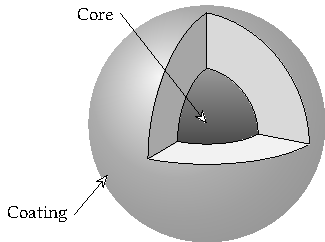
\includegraphics[scale=1]{lit_CCA}
  \caption{Schematic representation of concentric spheres of a two-phase composite}
  \label{fig:CCA}
\end{figure}
	
	It was shown that the differential equations of the CSA model (Fourier's transform law) could be used to incorporate additional phases in a spherical coordinate system~\autocite{Christensen.2012}. However, applying the continuity conditions on the interfaces and the boundary conditions on the outer surface creates a cumbersome process. By observing the repeating solutions of the differential equations in the middle rings, one could think of a recurring procedure. In~\parencite{Milton.2002}, such a procedure is introduced for particle-reinforced composites in which particle are covered with several coatings, see Fig.~\ref{fig:CCA2}. 

\begin{figure}[!h]
  \centering
  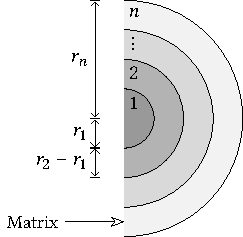
\includegraphics[scale=1]{lit_CCA2}
  \caption{A slice of several concentric hemispheres represented in 2D for multi-phase materials}
  \label{fig:CCA2}
\end{figure}	
	
	By adopting several concentric spheres (one sphere per phase), Eq.~\eqref{eq:cca} can be extended to $n$-phases:
	\begin{subequations}
	\begin{alignat}{2}
	k_{(1,2)}    &=k_2 + \frac{3p_1k_2}{p_2-\frac{3k_2}{k_2-k_1}},     \\
	k_{(1,2,3)}  &=k_3 + \frac{3p_{(1,2)}k_3}{p_2-\frac{3k_2}{k_2-k_{(1,2)}}},	\\
	k_{(1,2,3,4)}&=k_4 + \frac{3p_{(1,2,3)}k_4}{p_4-\frac{3k_4}{k_4-k_{(1,2,3)}}},	\\\nonumber
	\vdots\\
	k_{(1,2,\ldots,n)}&=k_n + \frac{3p_{( 1,2,\ldots,[n-1])}k_n}{p_n-\frac{3k_n}{k_n-k_{(1,2,\ldots,[n-1])}}}
	\end{alignat}
	\end{subequations}
	
	where $k_{(1,2,\ldots,n)}$ is the effective thermal conductivity of $n$ phases. One should notice that the number of required models/equations has reduced to $n-1$ with this method. Moreover, the fraction of each phase is defined as follows
	\begin{subequations}
	\begin{alignat}{3}
	p_{1} &= (\frac{r_1}{r_2})^3,&&&   p_{2}&=1-p{1},   \\
	p_{(1,2)} &= (\frac{r_1+r_2}{r_3})^3,&&&   p_{3}&=1-p{(1,2)},   \\
	p_{(1,2,3)} &= (\frac{r_1+r_2+r_3}{r_4})^3,&&&   p_{4}&=1-p{(1,2,3)},   \\\nonumber
	\vdots\\
	p_{(1,2,\ldots,n-1)} &= (\frac{\sum_{1}^{n-1}r_i}{r_n})^3,&&\qquad&   p_{n}&=1-p{(1,2,\ldots,n-1)},
	\end{alignat}
	\end{subequations}	
	where the last volume fraction $p_{(1,2,\ldots,n-1)}$ corresponds to the volume fraction of the reinforcements. One note that requires attention is that the outermost coating should always be the matrix.


\subsection{General Theory of Eigenstrains}
    Mura~\autocite*{Mura.1982} introduced the generic \textit{Eigenstrain} term for any stored (permanent) inelastic strains, which was inspired by Reißner's~\autocite*{Reissner.1931} classic work. The source of eigenstrains can be inhomogeneous inelastic deformations, plastic strains, creep strains, phase transformations, misfit strains, piezoelectric strains and temperature gradients among others. Thus, one great advantage of this generalization is that the all these different type of strains can be studied under one generic topic irrespective of their origin~\autocite{Jun.2010,Nyashin.2005}.

The general theory of eigenstrains deals with only two types of strains: elastic strains and eigenstrains. The main postulate of the theory is the additive decomposition of the actual strain (the total strain $\tenb{\varepsilon}^{\mupSigma}$): 
\begin{equation}
\tenb{\varepsilon}^{\mupSigma}=\tenb{\varepsilon}+\tenb{\varepsilon}^\eigen,\label{eq:eignestrains}
\end{equation}
where $\tenb{\varepsilon}$ is the elastic strain, and $\tenb{\varepsilon}^\eigen$ is the sum of all eigenstrains. Obviously, loading and unloading of an elastic stress-free body creates and removes elastic strains, respectively. Thus, eigenstrains (inelastic strains) are necessary but not enough to generate residual stresses. 

In classic continuum mechanics, the compatibility condition ensures that no overlap of the particles or gap between them happens in a continuum. The mathematical equivalent of this notion is Saint-Venant's compatibility theorem, which requires 
\begin{equation}
\curl{(\curl{\tenb{\varepsilon}})^\tran}=\nullb,\label{eq:saint}
\end{equation}
for an arbitrary tensor field $\tenb{\varepsilon}$ so that the respective displacement field $\tena{u}$ exists. The displacement field is found by solving the partial differential equation
\begin{equation}
\tenb{\varepsilon}=\gradsym{\tena{u}}.\label{eq:kinematics}
\end{equation}
In the presence of eigenstrains and by assuming a compatible elastic strain field, applying the compatibility condition to the total strain field results in
\begin{equation}
\curl{(\curl{\tenb{\varepsilon}})^\tran}=\curl{(\curl{\tenb{\varepsilon}^\eigen})^\tran}.\label{eq:sainttotal}
\end{equation}
    The right-hand side of this equation becomes non-zero for incompatible eigenstrains. By excluding the possibility of any gaps or overlaps, the incompatible eigenstrains give rise to eigenstresses. In this context, the incompatibility means that the strain field within the body cannot exist in a null stress state, i.e., an internal stress is required to enforce the strain field. This internal stress becomes present without any external force or constraints but only due to the necessity of satisfying kinematic conditions and the equilibrium equations. Such remaining internal stresses are the so-called \textit{residual stresses} in the engineering terminology, e.g., residual stresses due to fabrication and thermal stresses due to thermal expansion~\autocite{Hill.1996}. Two definitions of such residual stress is available in the literature:
\begin{enumerate}
\item Mura~\autocite*{Mura.1987} introduced a very restrictive definition: eigenstresses are self-equilibrated internal stresses, which are not caused by any external forces or constraints. Basically, any internal stress in the unloaded unconstrained body is an eigenstress.
\item Later, \citeauthor{Irschik.1988}~\autocite*{Irschik.1988} introduced the more relaxed concept of \textit{self-stress}, which is the internally equilibrated stress in the absence of external force but surface constraints are allowed.
\end{enumerate}
Herein, the first definition is adopted, and thus
\begin{equation}
\diver{\tenb{\sigma}^\eigen}=\nulla,\label{eq:eigenstressbalance}
\end{equation}
satisfies the equilibrium of the eigenstresses while
\begin{equation}
\tena{n}\scp\tenb{\sigma}^\eigen =\nulla,
\end{equation}
ensures a traction-free surface with an outward normal $\tena{n}$. 

Note that incompatible eigenstrains are the source of eigenstresses but not the other way around: incompatible eigenstrains generate elastic strains, which induce stress in the body~\autocite{Korsunsky.2017f}. The elastic strains are related to the total stress by Hooke's law:
\begin{equation}
\tenb{\sigma}^\mupSigma=\tend{C}\dscp \tenb{\varepsilon},\label{eq:eigenhooke}
\end{equation}
where $\tend{C}$ is the \textit{elastic tensor} or its inverse relation
\begin{equation}
\tenb{\varepsilon}=\tend{C}^\inv\dscp \tenb{\sigma}^\mupSigma,
\end{equation}
where $\tend{C}^\inv$ is the \textit{compliance tensor}.

In the free body condition (no external load and not constraints), the absence of eigenstrains indicates that there are no eigenstresses. In contrast, in the presence of eigenstrains, eigenstresses may or may not arise. The eigenstresses of the latter case are called \textit{impotent} or \textit{stress-free eigenstrains}, which are basically compatible or uniform strains. For instance, unconstrained uniform thermal strains are of this kind~\autocite{Korsunsky.2008}. 

\subsection{The Eshelby Method}
	The Eshelby method~\autocite{Eshelby.1957,Eshelby.1961} discusses the inclusion of ellipsoidal inhomogeneities within an infinite matrix. For the expense of incorporating an additional strain field around the inclusion, an equivalent homogeneous inclusion replaces the original inhomogeneity.\footnote{The `inhomogeneity' term implies that the inclusion is of a different material than the matrix whereas the `homogeneous' term implies that the inclusion is of the same material as the matrix. This is an interesting `thought experience'~\autocite[p.~89]{Clyne.2019} as it seems there is no justification for using the same material as of the matrix for the inclusion; mechanically there is not but mathematically there is.} Since the former has the same properties as of the matrix, the material discontinuity is thereby eliminated.
	
	Eshelby's \textit{equivalent inclusion method} takes advantage of a special impotent eigenstrain to transform the inhomogeneous inclusion to its equivalent homogeneous counterpart---the so-called `transformation strain'. To this end, the Eshelby tensor $\tenb{S}$ is introduced
	\begin{equation}
	\tenb{\varepsilon}^\text{C}=\tenb{S}\scp\tenb{\varepsilon}^\text{T},
	\end{equation}
	where $\tenb{\varepsilon}^\text{C}$ is the constrained strain and $\tenb{\varepsilon}^\text{T}$ is the transformation strain. Note that the Eshelby tensor depends only on the aspect ratio of the ellipsoidal inclusions. Once this tensor is known, the effective elastic tensor of the composites can be found~\autocite{Clyne.2019}:
	\begin{equation}
	\tend{C}_\text{eff}=\Big[(\tend{C}^\text{m})^\inv-\zeta_\text{f}\big[ (\tend{C}^\text{f}-\tend{C}^\text{m})\big(\tenb{S}-\zeta_\text{f}(\tenb{S}-\unitb)\big)+\tend{C}^\text{m}\big]^\inv(\tend{C}^\text{f}-\tend{C}^\text{m})(\tend{C}^\text{m})^\inv\Big]^\inv.
	\end{equation}
	One important assumption in this mean-field approach is that applying a far-field homogeneous strain to the composite induces a uniform strain in the inclusion~\autocite{Bohm.2020}. This implies a uniform stress for an elastic inclusion:
	\begin{subequations}
	\begin{align}
	\avevol{\tenb{\varepsilon}}^\text{(i)}&=\tenb{\varepsilon}^\text{(i)},\\
	\avevol{\tenb{\sigma}}^\text{(i)}&=\tenb{\sigma}^\text{(i)}.
	\end{align}
	\end{subequations}
	Note that this approach is valid for dilute composites. In the case of non-dilute composites, one way of taking into account the interaction of the fibres, is to introduce a background or image stress, which will be superimposed on the dilute stress field. Alternatively, the average of the disturbed strain field can be used. An analogous method is used in the following section to extend the Eshelby approach to heat transfer problems.

\subsection{The Hatta-Taya Model}
	There exist an analogy between various field values that are related by field theories. These theories usually assume a linear relationship that states the gradient of a field value is proportional to its dual; the constant of proportionality is usually a material property. From the representation theory point of view, another interpretation is possible, i.e., only the first-order terms of the generalised Taylor expansion is taken to represent the physical law. For instance in the context of elasticity, the stress is related to the gradient of deformation (strain) via the elastic tensor (Hooke's law); similarly in the heat transfer phenomenon, the gradient of temperature is related to heat flux via the thermal conductivity tensor (Fourier's law).

	Following the mentioned analogy, the Eshelby method, which was applied to obtain mechanical properties, was extended to acquire effective thermal properties in~\autocite{Hatta.1985}. Namely, the equivalent inclusion method was applied to heat transfer phenomena. Later, a similar approach was applied to coated inclusion~\autocite{Hatta.1986,Taya.1989}. In these studies, the assumption of dilute was released and the produced results remained in good agreements with the experimental ones up to 50\% fibre volume fraction as well as other method such the laminate analogy approach~\autocite{Fu.2003}. This latter approach categorises all the fibres---with the same orientation and length distributions---into a group that is modelled as a single laminate. Thus, the whole composite comprises of several laminates, i.e., a multi-directional laminar composite~\autocite{Callister.2018}. 	
	
	The Eshelby method in heat conduction establishes the equivalence between an inhomogeneity and its homogeneous counterpart by demanding the same heat flux through them.~\footnote{From a slightly different perspective, the principle of superposition can be used to additively decompose the heterogeneous media into a homogeneous problems and a deviation problem; this approach is common in Duhamel-Neumann type problems, see~\autocite{Javanbakht.2019b,Ghosh.2011,Oliver.2017}.} In non-dilute composite systems, the interaction of fibres are transferred through the matrix. In heat conduction, this is done by perturbing the temperature gradient field. Thus, the volume average of temperature gradient in the matrix ($\grad{\overline{T}}$) is selected as the disturbance measure of its respective field:
	\begin{equation}
		\grad{\overline{T}}=\int_{\text{D}-\mupOmega} \grad{T}^\text{T}-\grad{T}^0,
	\end{equation}
	where $\grad{T}^\text{T}$ is the total (actual) temperature gradient, $\grad{T}^0$ is the temperature gradient due to a uniform heat flux ($\tena{q}^0$) at infinity; and the matrix and inclusion domains are denoted by $\text{D}$ and $\mupOmega$, respectively.
	
	Similar to the transformation strain, the eigen-quantity of heat conduction is the transformation temperature gradient ($\grad{T}^*$) or sometimes called the eigen-temperature gradient~\autocite{Ghosh.2011}, which is used to set up a homogeneous domain. Analogously, an Eshelby tensor (usually called the S-tensor) for temperature gradient is also introduced:
	\begin{equation}
		\grad{T}^\text{C}=\tenb{S}\scp\grad{T}^*,
	\end{equation}
	where $\grad{T}^\text{C}$ is the constraint temperature gradient. The volume average of the transformation gradient, in 2D, is obtained from
	\begin{equation}
		\avevol{\grad{T}^*}_\mupOmega = \frac{1}{\zeta_{\text{f}}V_\text{D}}\int_{\mupOmega} \grad{T}^* \dif V = \frac{-\int_{-\alpha}^{\alpha} \grad{T}^*(\theta)\rho(\theta) \dif\theta}{\int_{-\alpha}^{\alpha} \rho(\theta) \dif\theta},
	\end{equation}
	where $\rho(\theta)$ is the number of fibres per unit area of the $\mathbb{S}^2$ unit sphere, and $V_\text{D}$ is the volume of the composite.
	
	Similar to the classic Eshelby tensor, the S-tensor depends on the geometry of the inclusions, which are modelled as spheroids with three semi-diameters $a_1$, $a_2$, and $a_3$ along the axis of the coordinate system $\left\{\tena{e}_i\right\}\equiv\left\{\tena{e}_i\right\}_{i=1}^3$. Short fibres are considered as oblate spheroids ($a_1=a_2\ll a_3$) in this model, and the components of the Eshelby tensor are explicitly calculated as
	\begin{subequations}
	\begin{alignat}{2}
		S_{11}=S_{22}&=\frac{\beta}{2\sqrt{(\beta^2-1)^3}}\left(\beta\sqrt{\beta^2-1}-\cosh^\inv\beta \right),\\
		S_{33}&=1-2S_{22},
	\end{alignat}
	\end{subequations}
	where $\beta\equidef\sfrac{a_3}{a_2}$ is the aspect ratio of the fibres. For isotropic fibres ($\tenb{k}_\text{f}\equiv k_\text{f}\unitb$) and matrix ($\tenb{k}_\text{m}\equiv k_\text{m}\unitb$), the auxiliary tensor
	\begin{equation}
		\tenb{A}\equidef (k_\text{f}-k_\text{m})\unitb\scp\tenb{S}+k_\text{m}\unitb,
	\end{equation}
	is used along with the Eshelby tensor to calculate
	\begin{subequations}
	\begin{alignat}{3}
		Q_1^*        &\equidef \frac{(k_\text{m}-k_\text{f})}{4\alpha}\left[ (2\alpha+\sin 2\alpha)      A_{11}^\inv+ (2\alpha-\sin 2\alpha)      A_{33}^\inv       \right],\\
		Q_3^*        &\equidef \frac{(k_\text{m}-k_\text{f})}{4\alpha}\left[ (2\alpha-\sin 2\alpha)      A_{11}^\inv+ (2\alpha+\sin 2\alpha)      A_{33}^\inv       \right],\\
		Q_1^\text{C} &\equidef \frac{(k_\text{m}-k_\text{f})}{4\alpha}\left[ (2\alpha+\sin 2\alpha)S_{11}A_{11}^\inv+ (2\alpha-\sin 2\alpha)S_{33}A_{33}^\inv       \right],\\
		Q_3^\text{C} &\equidef \frac{(k_\text{m}-k_\text{f})}{4\alpha}\left[ (2\alpha-\sin 2\alpha)S_{11}A_{11}^\inv+ (2\alpha+\sin 2\alpha)S_{33}A_{33}^\inv       \right],
	\end{alignat}
	\end{subequations}
	where $0\le \alpha\le\sfrac{\pi}{2}$ is the limit of the fibre angle. Finally, the axial (along the 3-axis) and transverse (along the 1-axis) effective properties are calculated by
	\begin{subequations}
	\begin{alignat}{2}
		k_{33} &= k_\text{m}\left( 1 - \frac{\zeta_{\text{f}}Q_3^*}{\zeta_{\text{f}}Q_3^\text{C}}   \right),\\
		k_{11} &= k_\text{m}\left( 1 - \frac{\zeta_{\text{f}}Q_1^*}{1+\zeta_{\text{f}}Q_1^\text{C}}   \right).
	\end{alignat}
	\end{subequations}
	
	
	\subsection{The Bound Approach}
	The most famous bounds for composite materials are the rule of mixtures (RoM) and the inverse rule of mixtures (IRoM). These two limits are merely special cases of Hill bounds. Other bounds are also available in the literature, which are mostly based on variational approaches. Namely, by applying the principles of minimum strain energy and minimum complementary strain energy the upper and lower extremes of the properties can be obtained, respectively. 
	
	The bound approach~\autocite{Nomura.1980} introduces tighter bounds compared to the RoM and IRoM. For the direction of fibres, the thermal conductivity is limited between
	\begin{subequations}
	\begin{alignat}{2}
	\left[\frac{\zeta_\text{f}}{k_\text{f}}+\frac{\zeta_\text{m}}{k_\text{m}}-\frac
	{\zeta_\text{f}\zeta_\text{m}(\frac{1}{k_\text{f}}-\frac{1}{k_\text{m}})^2h(\beta)}
	{(\zeta_\text{m}-\zeta_\text{f})(\frac{1}{k_\text{f}}-\frac{1}{k_\text{m}})h(\beta)+\frac{\zeta_\text{f}}{k_\text{f}}+\frac{\zeta_\text{m}}{k_\text{m}}}\right]^\inv\le k_\text{axial}\\
	k_\text{axial}\le
	\zeta_\text{f}k_\text{f}+\zeta_\text{m}k_\text{m}-\frac
	{\zeta_\text{f}\zeta_\text{m}(k_\text{f}-k_\text{m})^2\left(1-h(\beta)\right)}
	{(\zeta_\text{f}-\zeta_\text{m})(k_\text{f}-k_\text{m})[1-h(\beta)]+\zeta_\text{f}k_\text{f}+\zeta_\text{m}k_\text{m}}
	\end{alignat}
	\end{subequations}
	and in the transverse direction the limits
	\begin{subequations}
	\begin{alignat}{2}
	\left[\frac{\zeta_\text{f}}{k_\text{f}}+\frac{\zeta_\text{m}}{k_\text{m}}-\frac
	{2\zeta_\text{f}\zeta_\text{m}(\frac{1}{k_\text{f}}-\frac{1}{k_\text{m}})^2}
	{2(\zeta_\text{m}-\zeta_\text{f})(\frac{1}{k_\text{f}}-\frac{1}{k_\text{m}})+3(\frac{1}{k_\text{f}}+\frac{1}{k_\text{m}})}\right]^\inv\le k_\text{trans}\\
	k_\text{trans}\le
	\zeta_\text{f}k_\text{f}+\zeta_\text{m}k_\text{m}-\frac
	{\zeta_\text{f}\zeta_\text{m}(k_\text{f}-k_\text{m})^2}
	{(\zeta_\text{f}-\zeta_\text{m})(k_\text{f}-k_\text{m})+3(\zeta_\text{f}k_\text{f}+\zeta_\text{m}k_\text{m})}
	\end{alignat}
	\end{subequations}	
	with
	\begin{equation}
	h(\beta)=\frac{\beta}{\beta^2-1}\Big[1-\frac{1}{2}\Big(\sqrt{\frac{\beta}{\beta^2-1}}-\sqrt{\frac{\beta^2-1}{\beta}}\ln\frac{\beta+\sqrt{\beta^2-1}}{\beta-\sqrt{\beta^2-1}}\Big)\Big],
	\end{equation}
	were proposed where $\beta$ is the fibre aspect ratio; a wide range of spherical inclusions ($\beta=1$) to aligned fibres ($\beta\rightarrow\infty$) could be used that correspond to the two extreme values of $\sfrac{2}{3}\le h(\beta)\le1$, respectively. It can be seen that the fibre aspect ratio is deemed inconsequential in the transverse direction.






\section{Summary}
	The current chapter provides the necessary mathematical tools and concepts that are used in the development of the following chapters. A more specific literature, based on the case, is provided per chapter. Furthermore, the programming philosophy and the development of the used methodology are summarised in the following chapter; more details, such as the listing of the programming codes, are available in~\parencite{Javanbakht.2017}. 

\bl

	
	% s TODO non-local formulation
	%	Setting up a local model might result in very localised behaviour when softening behaviour is involved. One remedy is to use a non-local scheme by replacing the local strain field by its weighted average, which requires introducing a length parameter ($\ell$). So in the current model, the orientation is localised while the non-local strain field is used.

%\subsection{Direction-dependent Elastic and Bulk Moduli}
%	The direction-dependent elastic modulus 
%	\begin{equation}
%		E(\tena{d})=(\tena{d}^\tenpow{2}\dscp\tend{C}^\inv\dscp\tena{d}^\tenpow{2})^\inv,
%	\end{equation}
%	and the direction-dependent bulk modulus
%	\begin{equation}
%		K(\tena{d})=\frac{1}{3}(\unitb\dscp\tend{C}^\inv\dscp\tena{d}^\tenpow{2})^\inv,
%	\end{equation}
%	are evaluated with respect to the fixed arbitrary direction $\tena{d}$ where $\tend{C}^\inv$ is the elastic compliance tensor.



% --------------------------------------------------------------------------------------------------


%\subsection{Matrix Representation of a General 4th-order Tensor}
%	Often in order to carry out numerical analysis, the matrix presentation of tensors is required. For instance, general second- and fourth-order tensors can be arranged in terms of $3\times 3$ matrices (or $9\times 1$ column vectors) and $9\times 9$ matrices (or $81\times 1$ column vectors), respectively. Similarly, all tensorial operations should be translated to the algebra of matrices.
%
%
%\subsection{Matrix Representation of Elastic Tensor}
%	Fedorov's~\autocite{Fedorov.1968} representation of the elastic tensor $\tend{C}$ is obtained by using the orthonormal basis
%	\begin{subequations}
%	\begin{alignat}{2}
%		\tena{e}^\prime_1\equidef&\;&         \base_1\dyad&\base_1,\\
%		\tena{e}^\prime_2\equidef&\;&         \base_2\dyad&\base_2,\\
%		\tena{e}^\prime_3\equidef&\;&         \base_3\dyad&\base_3,\\
%		\tena{e}^\prime_4\equidef&\;&\sqrt{2}(\base_2\dyad&\base_3)^\sym,\\
%		\tena{e}^\prime_5\equidef&\;&\sqrt{2}(\base_1\dyad&\base_1)^\sym,\\
%		\tena{e}^\prime_6\equidef&\;&\sqrt{2}(\base_1\dyad&\base_1)^\sym,
%	\end{alignat}
%	\end{subequations}
%	to obtain an equivalent six-by-six elasticity matrix $\mat{C}$:
%	\begin{equation}\label{eq:fedorov}
%		\mat{C}_{ij} \equidef 	\tena{e}^\prime_i\scp\tend{C}\scp\tena{e}^\prime_j\qquad\qquad\forall i,j\in\{1,2,...,6\}.
%	\end{equation}
%	This matrix representation results in the following form of generalised Hooke's law:
%	
%	Note that Eq.~\eqref{eq:fedorov} is bridging between the tensorial and matrix notations. The introduced basis vectors are to ensure the equivalence between the following tensorial and matrix operations~\autocite{Nordmann.2018}:
%	
%	For the case of transversely isotropic material (hexagonal crystals), 5 material parameters plus the axis of symmetry must be known~\autocite{Bohlke.2001}.



%\pagebreak
% --------------------------------------------------------------------------------------------------


%\section{Classic Lamination Theory}
%    Classic lamination theory (CLT) is merely the extension of thin plate theory to accommodate laminates. It is based upon the following assumption~\autocite{Herakovich.1998}:
%    \begin{enumerate}
%        \item perfect inter-layer bonding exists,
%        \item each layer is homogeneous and can be orthotropic, transversely isotropic, or isotropic,
%        \item each layer is in the plane stress state~\footnote{In plane stress state, there exists a strain perpendicular to the plane of stress due to Poisson's effect, which will be ignored in the current context. Namely, no thickness change will be considered in CLT.}, and
%        \item the laminate deforms according to shear-rigid theory.
%    \end{enumerate}


    \input{./_Text/Methodology.tex}
    \input{./_Text/paper01.tex}
    \input{./_Text/paper02.tex}
    % !TeX root = ../my_thesis.tex
% !TeX spellcheck = en_GB
%!TEX TS-program = xelatex
%!BIB TS-program = biber

\chapter{Thermal Analysis of Natural Fibre Composites}\label{chap:p3}

\section*{Statement of Contribution}
	This chapter includes a co-authored book chapter. The bibliographic details of the published chapter are:
\begin{itemize}
	\item Javanbakht, Z, Hall, W \& Öchsner, A (2017), “Computational Evaluation of Transverse Thermal Conductivity of Natural Fiber Composites”, In: Improved Performance of Materials. Ed. by A Öchsner \& H Altenbach. Vol. 72. Advanced structured materials, Cham: Springer, pp. 197–206.
\end{itemize}
	My contribution as the corresponding author to the paper involved: undertaking literature review, classifying the necessary theoretical backgrounds and models, developing the programming code, analysing and discussing the finite element results, drawing figures, preparing tables, writing and editing the manuscript according to my supervisors’ comments.
	
\vspace{-0.5cm}
\Zia\\
\Wayne\\
\vfill
\newpage


\paragraph{Title:} Computational Evaluation of Transverse Thermal Conductivity of Natural Fiber Composites


\paragraph{Abstract.}The finite element analysis is used to investigate the sensitivity of the effective transverse thermal conductivity of polymeric composites reinforced with Manila hemp fibres in terms of their degree of saturation. It is predicted that the hierarchical structure of the fibre bundle will highly magnify the rate of water absorption and in consequence, the effective transverse thermal conductivity of the composite is altered. This influence is quantized in terms of the volume fraction of the fibre bundle and the lumen to produce a homogenized representative continuum. It was found that increasing the fibre volume fraction in a dry medium results in a decrease in the thermal conductivity whereas an increase of conductivity will be evident in a wet condition. Furthermore, the increase in the volume fraction of the lumen enhances the thermal conductivity by retaining more water during saturation which supports the developed hypothesis.

\section{Introduction}
	Natural fibres are widely used in various polymeric media for their typical low density, moderate cost, good specific strength, abundance and renewability of resources, and biodegradability among other favoured qualities. Nevertheless, the natural variability of properties, deficient fibre-to-matrix bonding, and more importantly their hydrophilic character introduce some challenges to their application. For instance, outdoor usage of natural composites is limited because of the susceptibility of their fibre reinforcements to environmental factors~\autocite{Assarar.2011,Placet.2009}.

	The porous structure of natural fibres makes them better thermal insulators compared to synthetic fibres such as glass or carbon~\autocite{Liu.2012}. On the other hand, their relatively low thermal conductivity may cause heat dissipation difficulties in some cases~\autocite{Kalaprasad.2000}. This trade-off attracted researchers in the past decades to investigate the naturally anisotropic thermal behaviour of these composites in terms of their volumetric composition~\autocite{Shah.2016}, volume fraction of fibres~\autocite{Li.2008}, fibre orientation~\autocite{Behzad.2007}, and thermal diffusivity~\autocite{Mangal.2003,Kalaprasad.2000} among other effective parameters.

	The mechanical properties of cellulose fibres are sensitive to the moisture content, particularly when incorporated into polymeric resins~\autocite{Faruk.2012}. Namely, the hygroscopic behaviour of natural fibres results in dimensional instabilities, i.e., swelling and shrinkage, which may induce residual stresses and microcracks into the composite as well as the debonding of the fibres~\autocite{Rakovsky.2014,Celino.2014}. From a macroscopic point of view, moisture initiates the degradation process of the natural fibres which in consequence, affects the properties of the composite. For instance, reduction of the elastic modulus and tensile strength~\autocite{Chow.2007,DHAKAL.2007}, fluctuation of the impact strength~\autocite{Athijayamani.2009}, and even the initiation of a fungal decay process~\autocite{Schirp.2007} is foreseeable. Herein, considering the porosity of the fibrous structure, it is hypothesised that the thermal conductivity of natural fibres is to be affected by the presence of water.
	
	Various theoretical and experimental methods were used to predict the thermal behaviour of natural fibres but the scarcity of the research on the effect of saturation motivated the current work, which is basically a computational effort to envision the big picture of the saturation process. In the current study, the effect of water content on the insulation role of a composite---reinforced with Manila hemp fibres in a high density polyethylene matrix---is investigated using the finite element method. A list of the used symbols in the current work is also provided, see Table~\ref{table:symbols4}.
\begin{table}[!h]
\centering
\caption{List of symbols}\label{table:symbols4}
\begin{tabular}{>{\centering}p{0.08\textwidth}p{0.78\textwidth}}
\toprule
$\gamma$ & mesh density\\
%$\zeta$ & volume fraction\\
$\zeta_{\text{f}}$ & volume fraction of the fibre bundle \red (volume of the solid part relative to that of the composite) \bl\\
$\zeta_{\text{l}}$ & volume fraction of the lumen \red (volume of the voids relative to that of the fibre bundle) \bl\\
$\mupDelta T$ &prescribed temperature gradient\\
$\ell$ & element edge length\\
$k_{\text{eff}}$ & effective thermal conductivity of the composite\\
$w$ &width of the RVE (the distance between the boundary faces)\\
$A_0$ &cross-sectional area perpendicular to direction of the flux\\
$\dot{Q}$ & total heat flux\\
$S_{\text w}$ &degree of saturation \\
$V_{\text f}$ & volume of the fibre bundle\\
$V_{\text{l}}$ & volume of the lumen (total voids) \\ 
$V_{\text w}$ & volume of the water\\
\bottomrule
\end{tabular}
\end{table}%


\begin{figure}[!b]
\centering
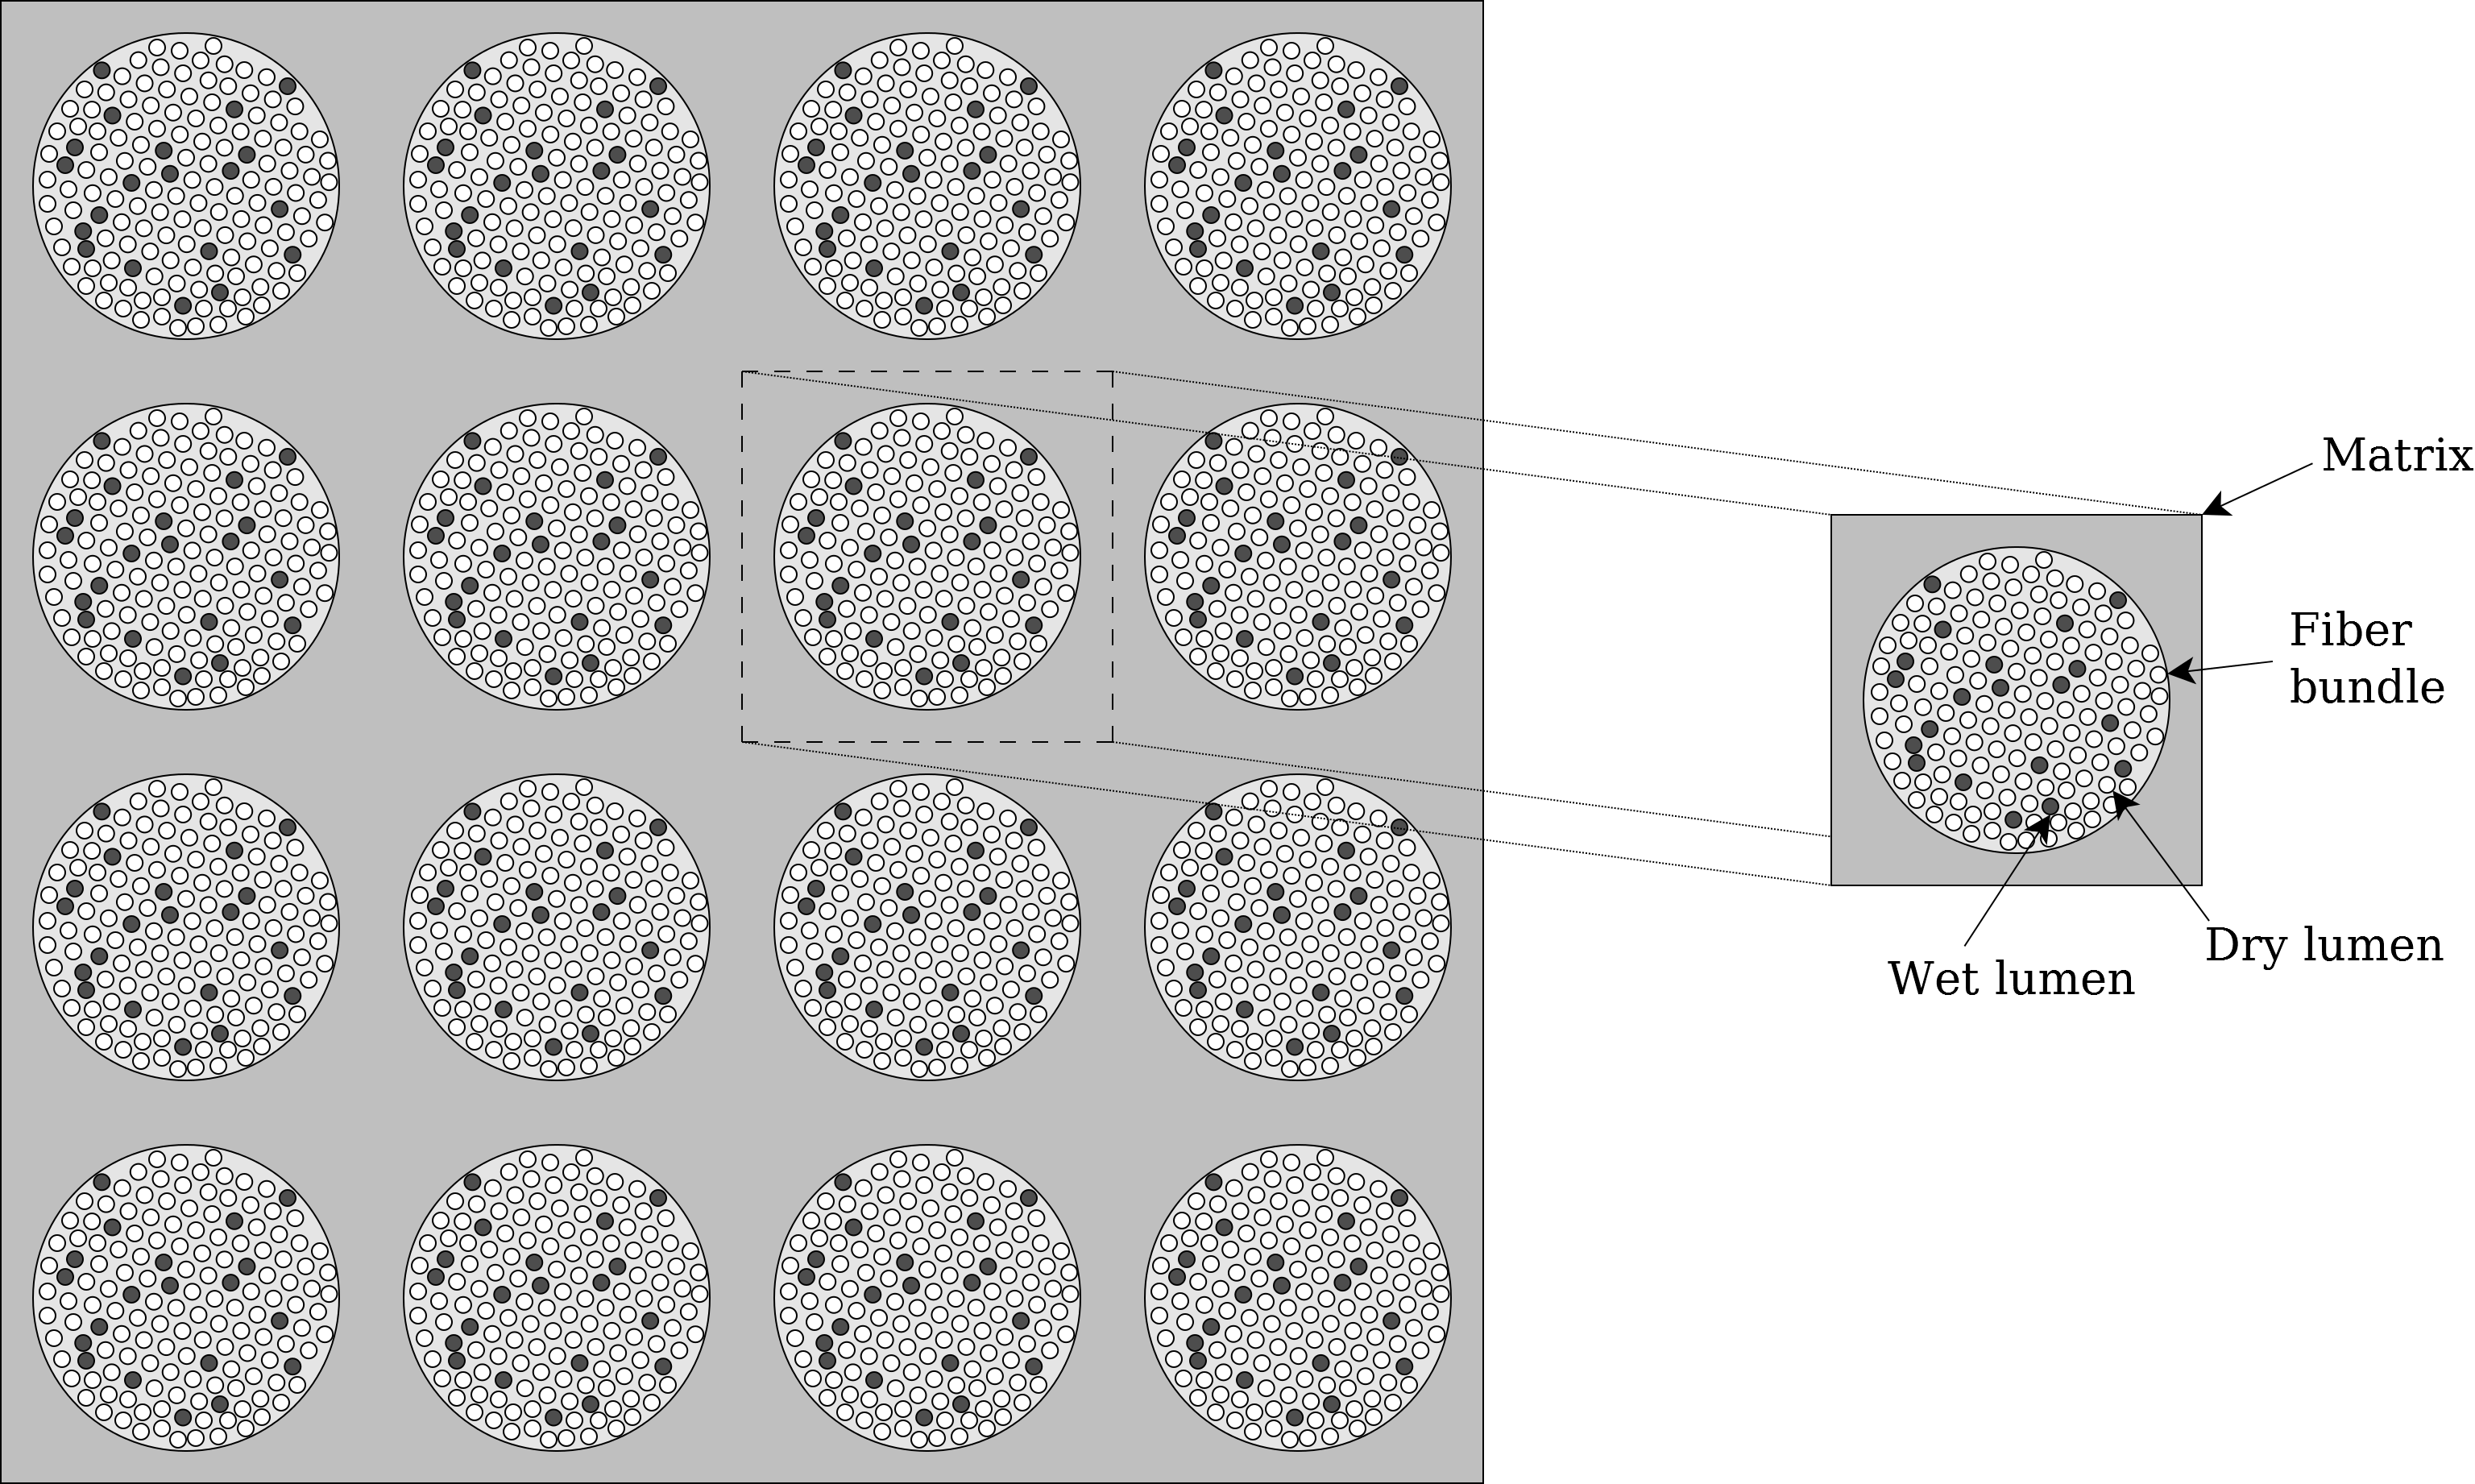
\includegraphics[width=\textwidth]{rve_heat}
\caption{Selected RVE from the unidirectional composite}\label{fig:rve}
\end{figure}


\red
\section{Composition of Natural Composites}
	\paragraph{Structure of hemp fibre composites} The composite is assumed to be made up of unidirectional hemp fibre bundles within a polymeric composite, see Fig.~\ref{fig:rve}. Each fibre bundle consists of a set of lumens, which are basically slender tubular structures that provide the air cavities~\autocite{Wang.2016}. Since the porosity of a natural fibre defines its capacity to hold water~\autocite{Rakovsky.2014}, the storage of moisture is done by filling the tubes with water and creating a wet lumen. Since no porosity is included in other components of the composite, lumens represent the total capacity of the fibre bundle to retain moisture. Dry lumens therefore provide the porosity whereas the remaining wet lumens hold the water in the composite.

\begin{figure}[!h]
\centering
\includegraphics[width=0.8\textwidth]{homo}
\caption{Homogenization process of the RVE}\label{fig:homo}
\end{figure}

	\paragraph{Components of the composite} A recent research shows that the bulk property of the fibrous structure can be properly modelled, within an acceptable margin of error, irrespective of the exact micro-level structure~\autocite{Liu.2011}. Therefore, a unit cell of the composite is selected as the RVE of the whole composite. In order to capture the hierarchy of the structure, the accumulated effect of the individual sub-structures are considered in four distinct layers: 
	\begin{enumerate}
	\item a polymeric matrix of high-density polyethylene (HDPE),
	\item the solid part of the Manila hemp fibre bundle,
	\item the water contained in the lumens, and
	\item the air which fills the remaining volume of the lumens.
	\end{enumerate}
	These four phases take part in the occurring thermal conduction process within the composite. The third phase vanishes in a 100\% dry fibre whereas the fourth phase is not available in completely saturated fibres.
	
	The thermal conductivities of the individual components of the composite are listed in Table~\ref{table:mat4}. This implies the fact that since the encapsulated water is stationary, no convection is taking place and the only means of heat transfer is the conduction mechanism~\autocite{Rakovsky.2014}.
	
\begin{table}[!bh]
\centering
\caption{Thermal conductivity of the composite components}\label{table:mat4}
\small
\begin{tabular}{p{0.2\textwidth}p{0.15\textwidth}p{0.4\textwidth}}
\toprule
\bfs{Component}&
\bfs{Material}&
\bfs{Conductivity} ($\scriptscriptstyle\frac{\text{W}}{\text{m}\cdot\text{K}}$)\\
\toprule
Matrix&
HDPE&
0.4025~\autocite{Rauwendaal.2014}\\
Solid fibre&
Hemp&
0.1847~\autocite{Liu.2011}\\
Lumen&
Air&
0.0026~\autocite{Liu.2011}\\
Moisture&
Water&
0.606~\autocite{Singh.2014}\\
\bottomrule
\end{tabular}
\end{table}	

	Finally, in the current study, the assumptions can be summarised into the following points:
	\begin{itemize}
		\item the porosity of the matrix and the solid portion of the hemp fibre bundle is neglected,
		\item all the porosity is provided by the lumens,
		\item the effect of the thermal barrier resistance is neglected,
		\item it is assumed that the thermal conductivity of the solid portion of hemp fibre bundles is independent of the lumen size,
		\item each component is assumed to be isotropic, and
		\item the thermal conductivity of all the components is assumed to remain constant by increasing the temperature.
	\end{itemize}
	As per these assumption, the following volume fractions can be defined:
	\begin{subequations}
	\begin{align}
	\zeta_{\text{f}}	&=\frac{V_{\text f}}{V_{\text c}},\\
	\zeta_{\text{l}}	&=\frac{V_{\text l}}{V_{\text f}},
	\end{align}
	\end{subequations}
	where $V_{\text f}$ is the volume of the whole fibre bundle, $V_{\text c}$ is the volume of the composite, $V_{\text l}$ is volume of the lumen, $\zeta_{\text{f}}$ is the volume fraction of the fibre bundle, $\zeta_{\text{l}}$ is the volume fraction of the lumen (relative to the volume of the fibre bundle). It is worth mentioning that the volume of the fibre bundle includes the solid volume plus dry and wet lumens. Namely, the fibre volume fraction is not only the fraction of the solid in the matrix.


	To represent the water content of the specimens, the degree of saturation~($S_{\text w}$) was used, which can be defined as follows:
\begin{equation}
S_{\text w}=\frac{V_{\text w}}{V_{\text{l}}},
\end{equation}
	where $V_{\text w}$ is the volume of the water, and $V_{\text{l}}$ is the volume of the lumen, which is equal to the total volume of the voids.
	




\red
\section{Micromechanical Model}
	Homogenisation of the continuous fibre-reinforced composites can be done by selecting a cylindrical RVE---which results in the so-called composite cylinder assemblage (CCA). This micromechanical model was first introduced in~\parencite{Hashin.1964} for evaluating the effective mechanical properties of hollow fibres within a matrix; the model is also called the composite spheres assemblage (CSA) and it is a two-phase model, i.e., a self-consistent model, which needs $n$-phase models for the same number of phases. Later, the mechanical properties of two-phase composite materials were considered in~\parencite{Christensen.1979} in a three-phase model. The latter effort marks the initial steps of the generalised self-consistent approach~\parencite{Bohm.2020} in which $n$-phase materials are modelled using $(n+1)$-phase models~\parencite{Herve.1993}. 
	
	By using several concentric cylinders in the CCA, each outer phase is modelled as a ring and the inner phase would be of a circular cross-section. Namely, the continuous fibres are replaced by a representative cross-section that implies the plain strain state for the problem. The homogenised medium would be of a circular cross-section that should admit to the boundary conditions of the original assembly. For instance in a thermal problem, two representations are linked together by enforcing the same temperature and heat flow on each of their boundaries. Originally, electrical conductivity of a two-phase composites was obtained in~\autocite{Kerner.1956b}. The same results of magnetic permeability of composite materials was obtained in~\autocite{Hashin.1962b} by means of variational principles. Later on, the interpretation of the latter resulted in the Hashin-Shtrikman bounds. 
	
	Herein, the CSA variant of the CCA model is adopted and extended to a four-phase composite in the context of thermal conductivity analysis. The CSA model was used to provide the benchmark values---the lower bound of the effective properties. It was shown that the differential equations of the CSA model (Fourier's transform law) could be used to incorporate additional phases in a spherical coordinate system~\autocite{Christensen.2012}. However, applying the continuity conditions on the interfaces and the boundary conditions on the outer surface creates a cumbersome process. By observing the repeating solutions of the differential equations in the middle rings, one could think of a recurring procedure. In~\parencite{Milton.2002}, such a procedure is introduced for particle-reinforced composites in which particle are covered with several coatings. By adopting several concentric spheres that represent each phase of four-phase natural fibre-reinforced composites, an analogous solution to the coated particles is readily obtained
	\begin{subequations}
	\begin{align}
		k_{\text{a-w}}     &= k_{\text{w}} + \frac{3(1-S_{\text{w}})k_{\text{w}}}{S_{\text{w}}-3\frac{k_{\text{w}}}{k_{\text{w}}-k_{\text{a}}}},\\\label{eq:airwater}
		k_{\text{a-w-f}}   &= k_{\text{f}} + \frac{3\zeta_{\text{l}}k_{\text{w}}}{1-\zeta_{\text{l}}-3\frac{k_{\text{f}}}{k_{\text{f}}-k_{\text{a-w}}}},\\
		k_{\text{a-w-f-m}} &= k_{\text{m}} + \frac{3\zeta_{\text{f}}k_{\text{w}}}{1-\zeta_{\text{f}}-3\frac{k_{\text{f}}}{k_{\text{f}}-k_{\text{a-w-f}}}},
	\end{align}
	\end{subequations}
	where `a', `w', `f', and `m' subscripts stand for air, water, fibre, and matrix, respectively. Thus, the effective thermal conductivity that results from the homogenisation of the air and water phases is denoted by $k_{\text{a-w}}$; a similar notation is used for the other two combinations. The four-phase micromechanical model can be readily solved by consecutive use of the CCA model for three times. By taking advantage of this approach, the $n$-phase model could be solved by $n-1$ equations/models.

\bl
\section{Methodology}
In the current study, the finite element method~\autocite{Ochsner.2013,Oechsner.2016} was used to estimate the effective thermal conductivity of unidirectional Manila hemp fibre bundles in the transverse (i.e., perpendicular to the principal fibre axis) direction. A four-phase continuum was created using the MSC.Marc (version 2014.2) commercial finite element package. This software was selected due to its capability of incorporating user-written pieces of code into its core algorithm. Namely, the customized procedures can be carried out using the subroutines written in the Fortran programming language~\autocite{Javanbakht.2017}. This facility---along with the provided Python scripting tool---makes it possible to fully automatize the parametric study~\autocite{Javanbakht.2016,Javanbakht.2016b}.

\red
	\paragraph{Mesh sensitivity} A 2D finite element model, with a thickness of the unit length, was created using a uniform mesh of elements of type 39, i.e., the 4-node bilinear isoparametric planar heat transfer elements. The uniform mesh density~($\gamma$) is defined using the following equation:
\begin{equation}
\gamma=\frac{1}{\ell_\text{mesh}},
\end{equation}
	where $\ell_\text{mesh}$ is the characteristic dimension of the element, i.e., the edge length of each square element. The used prototype for sensitivity analysis had a fibre volume fraction of 50\%, the typical lumen volume fraction of 30.87\%, and a water content of 25\%. Following several sensitivity analyses, a fluctuating of results was observed by refining the mesh. However, the mesh sensitivity was diminished for mesh densities over 300 and thus, a mesh density of 400 is used in the simulations, see Fig.~\ref{fig:sensitivty_hc1}. It is worth mentioning that the fibre overlap was allowed in all the simulation.

\begin{figure}[!h]{}
  \centering
	\includegraphics[scale=1]{hc1_mesh_sens}
  \caption{Sensitivity analysis of apparent thermal conductivity versus mesh density}
  \label{fig:sensitivty_hc1}
\end{figure}
\bl
	
	It is worth emphasizing that only one type of element was used with four different material properties, which represented the four distinct phases of the problem. Based on the volume fraction values of the fibre bundle and lumen plus the degree of saturation of the fibre, the occupied volume of each phase was calculated at the beginning of each analysis. In the next step, different properties were assigned to the elements by means of the \code{ANKOND} user subroutine. This subroutine is responsible for the anisotropic thermal behaviour of the material and it is called during the material assignments of the finite element analyses.
	
	Inasmuch as the prescribed temperature boundary conditions provide the most precise results in thermal conductivity analyses~\autocite{Islam.1999}, two set of prescribed temperatures were assigned to the left- and right-hand nodes of the RVE. Namely, a high temperature of $20^\circ\text{C}$ and a lower temperature of $0^\circ\text{C}$ were assigned as the boundary conditions. This established a temperature gradient, which was followed by a heat flux in the transverse direction, see Fig.~\ref{fig:sample}. The reaction heat flux of the lower temperature region was summed up and used to calculate the effective transverse thermal conductivity of the composite by means of Fourier's law~\autocite{Fiedler.2009}:
\begin{equation}
k_{\text{eff}}=\frac{\dot{Q}}{A_0}\cdot\frac{w}{\mupDelta T},
\end{equation}
	where $k_{\text{eff}}$ is the effective thermal conductivity of the composite, $\dot{Q}$ is the total reaction flux in the top boundary conditions, $A_0$ is the cross-sectional area perpendicular to direction of the flux, $w$ is the width of the RVE (distance between the boundary faces), and $\mupDelta T$ is the prescribed temperature difference.
\begin{figure}[t]
\centering
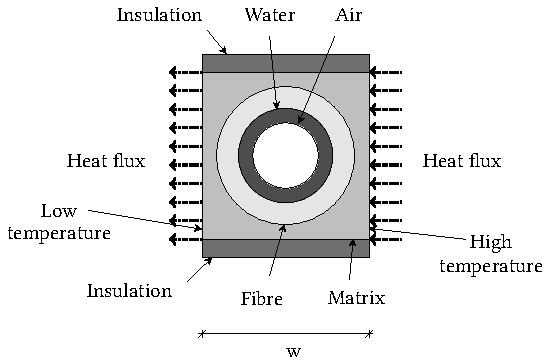
\includegraphics[width=0.6\textwidth]{chap4_fe}
\caption{Finite element model of the composite RVE}\label{fig:sample}
\end{figure}

\red
	\paragraph{Model validation} In order to validate the created prototype, the CSA model is used as the benchmark of the calculations. The typical value of 30.87\%~\autocite{Liu.2011} for the lumen volume fraction is taken along with the material properties listed in Table~\ref{table:mat4}. A range of fibre volume fraction from 10--50\% was taken to create Table~\ref{table:heat1_validation}; the effective thermal conductivity of the FE analyses and the CCA models are listed with the `RVE' and `CSA' subscripts, respectively. The percentage relative error ($e$) was calculated by deeming the CSA model as the benchmark. 

%\begin{table}[!h]
%\centering
%\caption{Simulation results of the mean thermal conductivity for various fibre volume fractions against the results of the CCA micromechanical model}\label{table:heat1_validation}
%\scriptsize
%\begin{tabular}{*{5}{P{0.06\textwidth}}}
%\toprule
%  \bfs{$\zeta_{\text{f}}$ (\%)}
%& \bfs{$S_{\text{w}}$ (\%)} 
%& \bfs{$k_\text{CCA}$} ($\scriptstyle\frac{\text{W}}{\text{m}\cdot\text{K}}$)
%& \bfs{$k_\text{RVE}$} ($\scriptstyle\frac{\text{W}}{\text{m}\cdot\text{K}}$)
%& \bfs{$e$ (\%)}
%\\
%\toprule
% 10 &0   &0.36542&	0.37984&	-3.95\\
% 10 &10  &0.36864&	0.38165&	-3.53\\
% 10 &20  &0.37157&	0.38338&	-3.18\\
% 10 &30  &0.37423&	0.38509&	-2.90\\
% 10 &40  &0.37667&	0.38652&	-2.62\\
% 10 &50  &0.37890&	0.38796&	-2.39\\
% 10 &60  &0.38096&	0.38936&	-2.20\\
% 10 &70  &0.38286&	0.39075&	-2.06\\
% 10 &80  &0.38463&	0.39194&	-1.90\\
% 10 &90  &0.38626&	0.39310&	-1.77\\
% 10 &100 &0.38779&	0.39427&	-1.67\\\midrule
% 20 & 0  &0.33054&	0.35845&	-8.44\\
% 20 &10  &0.33663&	0.36181&	-7.48\\
% 20 &20  &0.34218&	0.36523&	-6.74\\
% 20 &30  &0.34726&	0.36830&	-6.06\\
% 20 &40  &0.35192&	0.37109&	-5.45\\
% 20 &50  &0.35621&	0.37401&	-5.00\\
% 20 &60  &0.36018&	0.37670&	-4.59\\
% 20 &70  &0.36385&	0.37923&	-4.23\\
% 20 &80  &0.36727&	0.38167&	-3.92\\
% 20 &90  &0.37046&	0.38401&	-3.66\\
% 20 & 100&0.37344&	0.38624&	-3.43\\\midrule
% 30 & 0  &0.29768&	0.33813&	-13.59\\
% 30 &10  &0.30632&	0.34293&	-11.95\\
% 30 &20  &0.31423&	0.34772&	-10.66\\
% 30 &30  &0.32149&	0.35208&	-9.52\\
% 30 &40  &0.32818&	0.35637&	-8.59\\
% 30 &50  &0.33437&	0.36046&	-7.80\\
% 30 &60  &0.34011&	0.36426&	-7.10\\
% 30 &70  &0.34544&	0.36809&	-6.56\\
% 30 &80  &0.35042&	0.37162&	-6.05\\
% 30 &90  &0.35507&	0.37509&	-5.64\\
% 30 & 100&0.35942&	0.37831&	-5.25\\\midrule
% 40 & 0  &0.26668&	0.31873&	-19.52\\
% 40 &10  &0.27758&	0.32497&	-17.07\\
% 40 &20  &0.28760&	0.33101&	-15.09\\
% 40 &30  &0.29685&	0.33665&	-13.41\\
% 40 &40  &0.30540&	0.34221&	-12.05\\
% 40 &50  &0.31334&	0.34741&	-10.87\\
% 40 &60  &0.32072&	0.35249&	-9.91\\
% 40 &70  &0.32761&	0.35714&	-9.02\\
% 40 &80  &0.33404&	0.36186&	-8.33\\
% 40 &90  &0.34008&	0.36627&	-7.70\\
% 40 & 100&0.34574&	0.37054&	-7.17\\\midrule
% 50 & 0  &0.23736&	0.30036&	-26.54\\
% 50 &10  &0.25029&	0.30796&	-23.04\\
% 50 &20  &0.26222&	0.31504&	-20.15\\
% 50 &30  &0.27326&	0.32202&	-17.84\\
% 50 &40  &0.28352&	0.32854&	-15.88\\
% 50 &50  &0.29306&	0.33483&	-14.25\\
% 50 &60  &0.30198&	0.34092&	-12.90\\
% 50 &70  &0.31031&	0.34675&	-11.74\\
% 50 &80  &0.31813&	0.35239&	-10.77\\
% 50 &90  &0.32547&	0.35778&	-9.93\\
% 50 & 100&0.33237&	0.36302&	-9.22\\
% \bottomrule
%\end{tabular}
%\end{table}

\renewcommand{\arraystretch}{0.7}
\begin{table}[!h]
\centering
\caption{Simulation results of the mean thermal conductivity for various fibre volume fractions against the results of the CSA micromechanical model}\label{table:heat1_validation}
\small
\begin{tabular}{*{2}{P{0.08\textwidth}}*{2}{P{0.1\textwidth}}P{0.08\textwidth}}
\toprule
  \bfs{$\zeta_{\text{f}}$ (\%)}
& \bfs{$S_{\text{w}}$ (\%)} 
& \bfs{$k_\text{CSA}$} ($\scriptstyle\frac{\text{W}}{\text{m}\cdot\text{K}}$)
& \bfs{$k_\text{RVE}$} ($\scriptstyle\frac{\text{W}}{\text{m}\cdot\text{K}}$)
& \bfs{$e$ (\%)}
\\
\toprule
 10 &0   &0.36542&	0.37984&	-3.95\\
 10 &10  &0.36864&	0.38165&	-3.53\\
 10 &20  &0.37157&	0.38338&	-3.18\\
 10 &30  &0.37423&	0.38509&	-2.90\\
 10 &40  &0.37667&	0.38652&	-2.62\\
 10 &50  &0.37890&	0.38796&	-2.39\\
 10 &60  &0.38096&	0.38936&	-2.20\\
 10 &70  &0.38286&	0.39075&	-2.06\\
 10 &80  &0.38463&	0.39194&	-1.90\\
 10 &90  &0.38626&	0.39310&	-1.77\\
 10 &100 &0.38779&	0.39427&	-1.67\\\midrule
 20 & 0  &0.33054&	0.35845&	-8.44\\
 20 &10  &0.33663&	0.36181&	-7.48\\
 20 &20  &0.34218&	0.36523&	-6.74\\
 20 &30  &0.34726&	0.36830&	-6.06\\
 20 &40  &0.35192&	0.37109&	-5.45\\
 20 &50  &0.35621&	0.37401&	-5.00\\
 20 &60  &0.36018&	0.37670&	-4.59\\
 20 &70  &0.36385&	0.37923&	-4.23\\
 20 &80  &0.36727&	0.38167&	-3.92\\
 20 &90  &0.37046&	0.38401&	-3.66\\
 20 & 100&0.37344&	0.38624&	-3.43\\\midrule
 30 & 0  &0.29768&	0.33813&	-13.59\\
 30 &10  &0.30632&	0.34293&	-11.95\\
 30 &20  &0.31423&	0.34772&	-10.66\\
 30 &30  &0.32149&	0.35208&	-9.52\\
 30 &40  &0.32818&	0.35637&	-8.59\\
 30 &50  &0.33437&	0.36046&	-7.80\\
 30 &60  &0.34011&	0.36426&	-7.10\\
 30 &70  &0.34544&	0.36809&	-6.56\\
 30 &80  &0.35042&	0.37162&	-6.05\\
 30 &90  &0.35507&	0.37509&	-5.64\\
 30 & 100&0.35942&	0.37831&	-5.25\\\midrule
 40 & 0  &0.26668&	0.31873&	-19.52\\
 40 &10  &0.27758&	0.32497&	-17.07\\
 40 &20  &0.28760&	0.33101&	-15.09\\
 40 &30  &0.29685&	0.33665&	-13.41\\
 40 &40  &0.30540&	0.34221&	-12.05\\
 40 &50  &0.31334&	0.34741&	-10.87\\
 40 &60  &0.32072&	0.35249&	-9.91\\
 40 &70  &0.32761&	0.35714&	-9.02\\
 40 &80  &0.33404&	0.36186&	-8.33\\
 40 &90  &0.34008&	0.36627&	-7.70\\
 40 & 100&0.34574&	0.37054&	-7.17\\\midrule
 50 & 0  &0.23736&	0.30036&	-26.54\\
 50 &10  &0.25029&	0.30796&	-23.04\\
 50 &20  &0.26222&	0.31504&	-20.15\\
 50 &30  &0.27326&	0.32202&	-17.84\\
 50 &40  &0.28352&	0.32854&	-15.88\\
 50 &50  &0.29306&	0.33483&	-14.25\\
 50 &60  &0.30198&	0.34092&	-12.90\\
 50 &70  &0.31031&	0.34675&	-11.74\\
 50 &80  &0.31813&	0.35239&	-10.77\\
 50 &90  &0.32547&	0.35778&	-9.93\\
 50 & 100&0.33237&	0.36302&	-9.22\\
 \bottomrule
\end{tabular}
\end{table}
\renewcommand{\arraystretch}{1}
	
	It was observed that by increasing the fibre volume fraction, the relative error increases from a minimum of 1.77\% to a maximum of 26.54\%. The RVE seemed to slightly overestimate the effective thermal conductivity. Moreover, by increasing the water content, the FE values approach the values of the CSA model. Overall, the FE prototype showed an acceptable range of errors. Nevertheless, the results of the analyses with lower volume fractions seemed to be closer to the lower bound provided by the CSA model.
\afterpage{\clearpage}
\bl

\section{Results and Discussion}
	In a typical hemp fibre, the average diameter of the fibre bundle and lumens are 213 and 16.5 microns, respectively. Also an average number of 137 lumens exists in every fibre bundle, which results in an average lumen volume fraction of 30.87\%\,\footnote{\red Note that the calculation of average lumen fraction was carried out in this reference based on a histogram, and thus the reported average numbers will not results in the value of 30.87\%; see the reference~\autocite{Liu.2011} for further details.\bl}~\autocite{Liu.2011}. The saturation of this typical hemp fibre was simulated and the effective transverse thermal conductivity of the composite was calculated using the accumulated reaction heat fluxes, see Fig.~\ref{fig:typical}.
	
\begin{figure}[!h]
  \centering
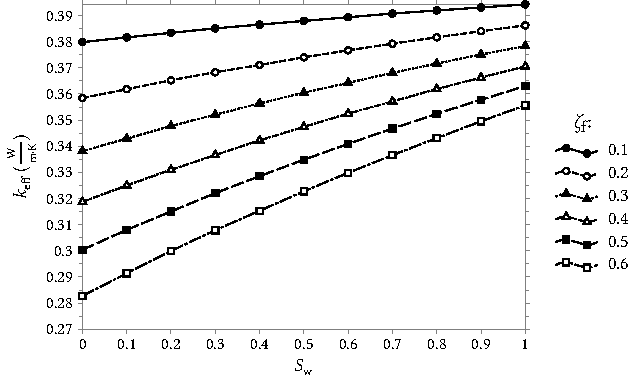
\includegraphics[scale=1]{typical}
  \caption{Effective transverse thermal conductivity of a typical lumen fraction ($\zeta_{\text{l}}=30.87\%$)}
  \label{fig:typical}
\end{figure}

	\red 
	As mentioned earlier, increasing the volume fraction adds to the amount of both the solid and lumen components. Therefore by increasing the fibre volume fraction, a completely dry fibre loses its thermal conductivity. This is due to the lower thermal conductivity of both fibre and air with respect to the matrix; thus, an isolation effect in dry fibre is expected. On the other hand, by increasing the fibre volume fraction in completely saturated fibres a milder isolation is obtained. This can be attributed to the thermal conductivity of water, which is higher than that of the matrix, and works in the opposite direction of fibre increase.\bl


	Furthermore in Fig.~\ref{fig:typical}, it can be noted that by increasing the degree of saturation, the effective thermal conductivity experiences an increase, which happens at a higher rate for the higher fibre bundle volume fractions. For instance, for a fibre bundle volume fraction of 60\%, the saturation causes an increase of the thermal conductivity by 25.79\% whereas the same value was only improved by 3.79\% for a volume fraction of 10\%. In other words, although the lumen fraction is kept constant, the amount of absorbed water increases due to the overall increase in the cross-sectional area of the fibre bundle.
	
	The effect of lumen volume fraction is investigated for two extreme fibre bundle volume fractions, i.e., a high volume fraction of 60\% and low volume fraction of 10\%, see Figs.~\ref{fig:low} and \ref{fig:high}. Increasing the lumen volume fraction in either case results in an increase in the effective thermal conductivity due to saturation. This effect is augmented at higher fibre bundle volume fractions. For example, the complete saturation of a low fibre content composite with a small lumen volume fraction increases the transverse thermal conductivity by only 1.24\% whereas a high content fibre with a high lumen volume fraction undergoes a 44.61\% improvement.

	
\begin{figure}[!h]{}
  \centering
 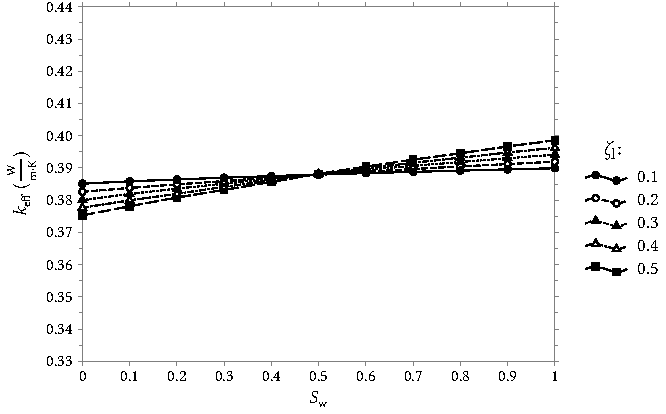
\includegraphics[scale=1]{low}
  \caption{Effective transverse thermal conductivity of low fibre volume fraction composite ($\zeta_{\text{f}}=10\%$)}
  \label{fig:low}
\end{figure}

\begin{figure}[!h]{}
  \centering
 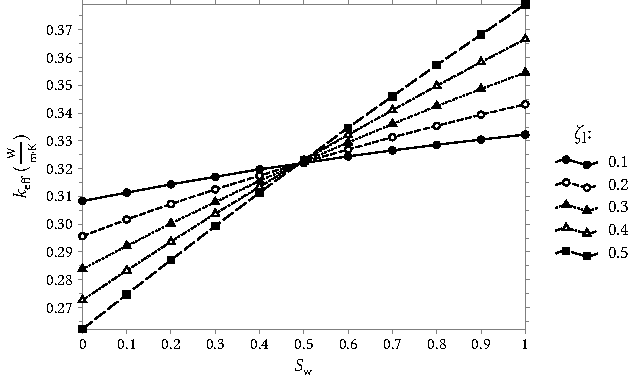
\includegraphics[scale=1]{high}
  \caption{Effective transverse thermal conductivity of high fibre volume fraction composite ($\zeta_{\text{f}}=60\%$)}
  \label{fig:high}
\end{figure}

\red
	One interesting point in both Figs.~\ref{fig:low} and \ref{fig:high} is the fact that around 50\% saturation, all lumen volume fractions result in the same apparent thermal conductivity. This could be justified by the setup of the FE model; the water component has a relatively high thermal conductivity and it surrounds the air phase in the middle, see Fig.~\ref{fig:sample}. It seems that the saturations around 50\% could redirect the heat flow around the air phase irrespective of the lumen volume fraction. From another point of view, by observing Eq.~\eqref{eq:airwater}, one could see that the contribution of the water-air phase depends only on the degree of saturation.\,\footnote{This statement implies that the thermal conductivities are assumed to be constant.} Nevertheless, this outcome requires further investigations, e.g., an experimental validation.
\bl

	In the dry composite samples, increasing the fibre bundle volume fraction reduces the effective thermal conductivity for a specific lumen volume fraction. Similarly, increasing the lumen volume fraction for a specific fibre bundle volume fraction, decreases the thermal conductivity of the specimen, see Fig.~\ref{fig:dry}. On the other hand, in a fully saturated composite sample, the effect is opposite to that of the dry sample due to the higher thermal conductivity of the absorbed water compared to air, see Fig.~\ref{fig:saturated}.
\begin{figure}[!h]{}
  \centering
 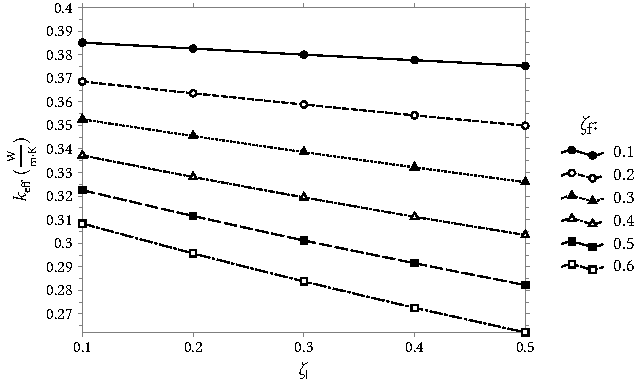
\includegraphics[scale=1]{dry}
  \caption{Effective transverse thermal conductivity of dry composite specimens}
  \label{fig:dry}
\end{figure}

\begin{figure}[!h]{}
  \centering
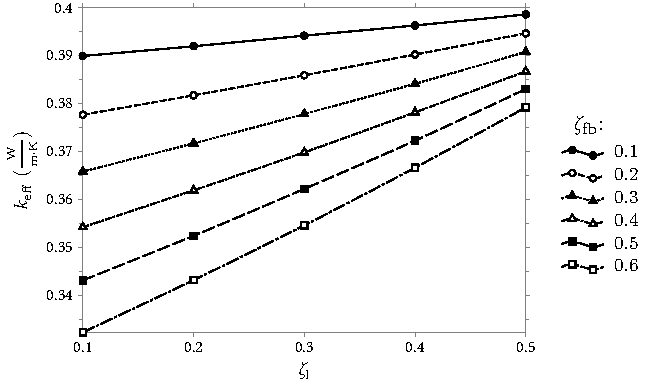
\includegraphics[scale=1]{sat}
  \caption{Effective transverse thermal conductivity of fully saturated composite specimens}
  \label{fig:saturated}
\end{figure}
\newpage
\section{Conclusion}
\red
	In summary, an FE model was introduced for evaluating the apparent/effective thermal conductivity of the Manila hemp fibres---this method, however, is applicable to every type of natural fibre composites. After validating the FE model with the composite spheres assemblage model, a typical case was analysed. It was shown that dry fibres have an isolation effect, which becomes more pronounced at higher fibre volume fractions. A milder isolation was observed for the fully saturated state.\bl\ It was shown the porosity of the Manila hemp fibre bundles affected the effective transverse thermal conductivity of the natural composite. Namely, by increasing the lumen fraction, a decrease was observed in the dry samples whereas an improvement happened in the effective thermal conductivity of the fully saturated samples. This effect was highly augmented in high fibre bundle volume fractions since the amount of water absorption was increased due to the increased volume of the voids within the fibre bundle. In consequence, the effective transverse thermal conductivity of the composite was increased. \red\ In future studies, carefully-controlled experimental studies should be conducted to refine the possible shortcomings of the FE model, e.g., the mesoscopic heat flow around 50\% saturation.\bl




    \input{./_Text/paper04.tex}
    % !TeX spellcheck = en_GB
%!TEX TS-program = xelatex
%!BIB TS-program = biber
\chapter{Thermal Analysis of Orientation Clustering}\label{chap:p5}
\section*{Statement of Contribution}
	This chapter includes a co-authored book chapter. The bibliographic details of the published chapter are:
\begin{itemize}
	\item Javanbakht, Z, Hall, W \& Öchsner, A (2019), “Effective Thermal Conductivity of Fibre Reinforced Composites Under Orientation Clustering”, In: Engineering design applications. Ed. by A Öchsner \& H Altenbach. Vol. 92. Advanced structured materials, 1869-8433, Cham, Switzerland: Springer, pp. 507–519.
\end{itemize}
	My contribution as the corresponding author to the paper involved: undertaking literature review, classifying the necessary theoretical backgrounds and models, developing the programming code, analysing and discussing the finite element results, drawing figures, preparing tables, writing and editing the manuscript according to my supervisors’ comments.

\Zia\\
\Wayne\\
\vfill
\newpage

% --------------------------------------------------------------------------------------------------
\paragraph{Title} Effective Thermal Conductivity of Fibre Reinforced Composites Under Orientation Clustering

\paragraph{Abstract} A parametric finite element analysis is carried out to investigate the sensitivity of the effective thermal conductivity of fibres to orientation clustering. Randomly-positioned fibres with von Mises orientation distributions were used in different considerations and volume fractions to generate the dispersion in a partitioned representative volume element. It was found that increasing the fibre volume fraction increases the thermal conductivity; this improvement is significant specially when a preferred orientation is detected with a cluster-free state. Further reinforcement of the composite is made possible by increasing the maximum principal value of the orientation tensor provided that the principal direction is set accordingly. Furthermore, clustering index seems to not be affected by volume fraction when an equal distribution is present in partitions.

\section{Introduction}
	Heat dissipation can be problematic in composites due to their low thermal conductivity and anisotropic nature~\autocite{Kalaprasad.2000}. There are several parameters which affect the thermal conductivity of fibre reinforced composites among which is the orientation of the fibres; it plays a key role in defining the internal structure of the composite~\autocite{Behzad.2007,Lee.2003}. Additionally, increasing the fibre volume fraction will initiate more interaction between the fibres specially in the concentrated regions. The effect of these two parameters couples together in non-dilute regions of moulding flows during injection moulding processes, i.e., volume fractions more than 1\% are more susceptible to fibre clustering~\autocite{Ranganathan.1990}. Further complication is introduced when the effect of interfacial thermal barrier resistance is considered. Namely, not merely the volume fraction but also the specific area of the inclusions is also influential~\autocite{Hasselman.1987}.
	
	Due to the aforementioned complications, among many others, evaluation of the thermal conductivity of various fibres of composites has been an attraction to researchers. Effective thermal conductivity of fibres in the transverse direction~\autocite{Liu.2012,Agrawal.2015,Qian.2016,Javanbakht.2018}, in-plane~\autocite{Villiere.2013,Behzad.2007}, and longitudinal direction~\autocite{Korab.2002,Yang.2005} has been investigated in the literature. Furthermore, three dimensional pseudo-random distribution of fibres is considered in~\autocite{Wang.2009,GomezMunoz.2008,Javanbakht.2016,Javanbakht.2016b,Kari.2007}. The anisotropic improvement of heat conduction is also investigated in several publications, see~\autocite{Tian.2012,Gori.2013}. Many of the analytical approaches tend to provide wide bounds, specially for high contrast heterogeneous media, rather than specific values~\autocite{Kanit.2003}. In addition, high contrast fibre reinforced composites show more sensitivity to clustering~\autocite{Kataoka.2000}. Therefore in this context, computational methods are favoured despite the fact that the results are more model-dependent. Such side effects should be smoothed by selecting appropriate representative volume elements (RVEs) and explicit consideration of fibre orientation.
	
	The orientation of fibres in a composite can be described statistically in a continuous manner using orientation distribution functions~\autocite{Nomura.1970}. The discretised alternative is using orientation tensors~\autocite{Scheidegger.1965,Advani.1987} which are evaluated for various regions of the medium to detect orientation clustering of fibres~\autocite{Lee.2003,Krause.2010,Sliseris.2016,Yang.2010}. Many high order orientation tensors are available in the literature~\autocite{DuChung.2002} but the second order orientation tensor is more frequent due to its simplicity. Although a second order orientation tensor is not deemed accurate enough to represent the micro-structure of a composite~\autocite{Muller.2016b}, it is adequate for calculations pertaining to thermal conductivity~\autocite{Ranganathan.1990}.
	
	In the current study, a mean field approach is adopted to correlate the effect of clustered fibres to the effective thermal conductivity. Computational analyses were carried out using the finite element method. Most of the numerical researches have used auxiliary programming languages, such as Mathematica~\autocite{GomezMunoz.2008}, to carry out the generation of pseudo-random fibre distribution. This requires a transfer of data between programs and some manual handling of the operations. Herein, an integrated Python script is used along with the MSC Marc commercial finite element package in a manner that the connection is automatically established and maintained. Furthermore, all supplementary calculations and post-processing tasks were handled by means of the same facility, for detailed information see \autocite{Javanbakht.2017}. A list of the used symbols in the current work is also provided for the convenience of the reader, see Table~\ref{table:symbols5}.
\begin{table}[!h]
\centering
\caption{List of used symbols}\label{table:symbols5}
\begin{tabular}{>{\centering}p{0.1\textwidth}>{\small}p{0.85\textwidth}}
\toprule\noalign{\smallskip}
$\gamma$             & uniform mesh density\\
$\vartheta^\prime$   & rotation of the principal direction transformation\\
$\zeta_{\text{f}}$  & volume fraction of the fibre\\
$\lambda_i$        & $i$-th eigenvalue\\
$\mu$              & mean value of the von Mises distribution\\
$\kappa$           & concentration parameter of the von Mises distribution\\
$\psi$             & probability distribution function\\
$\mupDelta T$       & prescribed temperature gradient\\
$\mupDelta z$         & length over which temperature gradient is formed (the distance between the boundaries)\\
$\ell_\text{mesh}$                & element edge length\\
$k_{\text{eff}}$   & effective thermal conductivity of the composite\\
$k_{\text{f}}$     & thermal conductivity of the fibre\\
$k_{\text{m}}$     & thermal conductivity of the matrix\\
$A_0$              & cross-sectional area perpendicular to direction of the flux\\
$\dot{Q}$          & total heat flow\\
$\tena{e}_i$       & orthonormal unit basis\\
$\tena{e}_i^\prime$     & orthonormal unit basis of the principal direction\\
$\tena{d}$         & fibre direction vector\\
$\tenb{H}$         & orientation second-order tensor\\
$\tenb{H}^\prime $      & orientation second-order tensor (spectral form)\\
$\tenb{Q}$         & transformation second-order tensor\\
\noalign{\smallskip}\bottomrule\noalign{\smallskip}
\end{tabular}
\end{table}%

% ══════════════════════════════════════════════════════════════════════════════════════════════════
% Eigenvalue Analysis of Orientation Tensors
% ══════════════════════════════════════════════════════════════════════════════════════════════════
%TODO the whole section must be rephrased
\section{Eigenvalue Analysis of Spherical Distributions}
	The direction of every short fibre can be indicated by a unit vector ($\tena{d}\equiv\tena{d}(\vartheta,\varphi)$), see Fig.~\ref{fig:vector5}. The locus of the end points of such vectors is the surface of a unit sphere in 3D space---a spherical distribution. Considering fibres as the reinforcements of the composite makes the direction of them insignificant, i.e., both $\tena{d}$ and $-\tena{d}$ will have the same reinforcing effect. Therefore, the locus of the end points will reduce to a unit hemisphere in 3D or a unit half circle in 2D. Namely, in a 2D Euclidean coordinate system, one degree of freedom is enough to specify the orientation of a fibre, i.e., $\tena{d}\equiv\tena{d}(\varphi)$.

\begin{figure}[!h]
\tdplotsetmaincoords{60}{110}
\centering
%\begin{tikzpicture}[scale=4,tdplot_main_coords]
%%define polar coordinates for some vector
%\pgfmathsetmacro{\rvec}{1.2}
%\pgfmathsetmacro{\varthetavec}{40}
%\pgfmathsetmacro{\varphivec}{50}
%
%\coordinate (O) at (0,0,0);
%
%%determine a coordinate (P) using (r,\vartheta,\varphi) coordinates.  This command
%%also determines (Pxy), (Pxz), and (Pyz): the xy-, xz-, and yz-projections
%%of the point (P).
%%syntax: \tdplotsetcoord{Coordinate name without parentheses}{r}{\vartheta}{\varphi}
%\tdplotsetcoord{P}{\rvec}{\varthetavec}{\varphivec}
%\tdplotsetcoord{Punit}{\rvec/3}{\varthetavec}{\varphivec}
%
%%draw figure contents
%%--------------------
%
%%draw the main coordinate system axes
%\draw[thick,->] (0,0,0) -- (1,0,0) node[anchor=north east]{$1$};
%\draw[thick,->] (0,0,0) -- (0,1,0) node[anchor=west]{$2$};
%\draw[thick,->] (0,0,0) -- (0,0,1) node[anchor=south]{$3$};
%
%%draw a vector from origin to point (P) 
%\draw[color=black!50,line width=0.2cm] (O) -- (P) node [color=black,above=-0.1cm] {Fibre};
%\draw[color=black,dash dot] (O) -- (P);
%\draw[-stealth,very thick, label=fibre] (O) -- (Punit) node [below right] {$\tena{d}$};
%
%%draw projection on xy plane, and a connecting line
%\draw[dashed] (O) -- (Pxy);
%\draw[dashed] (P) -- (Pxy);
%
%%draw the angle \varphi, and label it
%%syntax: \tdplotdrawarc[coordinate frame, draw options]{center point}{r}{angle}{label options}{label}
%\tdplotdrawarc{(O)}{0.2}{0}{\varphivec}{anchor=north}{$\varphi$}
%
%
%%set the rotated coordinate system so the x'-y' plane lies within the
%%"theta plane" of the main coordinate system
%%syntax: \tdplotsetthetaplanecoords{\varphi}
%\tdplotsetthetaplanecoords{\varphivec}
%
%%draw theta arc and label, using rotated coordinate system
%\tdplotdrawarc[tdplot_rotated_coords]{(0,0,0)}{0.5}{0}{\varthetavec}{anchor=south west}{$\vartheta$}
%
%%draw some dashed arcs, demonstrating direct arc drawing
%%\draw[dashed,tdplot_rotated_coords] (\rvec,0,0) arc (0:90:\rvec);
%%\draw[dashed] (\rvec,0,0) arc (0:90:\rvec);
%\end{tikzpicture}
 	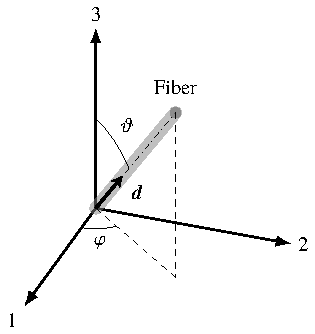
\includegraphics[scale=1]{direction_vector}
\caption{Representation of the orientation of a general fibre in the 3D space using a unit vector $\tena{d}$}\label{fig:vector5}
\end{figure}%
	
	Using the summation convention, the representative planar unit vector of a fibre is denoted as:
	\begin{equation}
	\tena{d}=d_i\tena{e}_i,\qquad i=1,2,
	\end{equation}
	where $\tena{e_i}$ is the $i$-th basis unit vector of the coordinate system, and  $d_i$ is the $i$-th component of the unit vector $\tena{d}$.

The 2nd-order planar orientation tensor ($\tenb{H}$) can be defined as~\autocite{Advani.1987}:
\begin{equation}\label{eq:one5}
H_{ij}=\int_{0}^{2\uppi}\psi(\varphi)d_id_j\text{d}\varphi,
\end{equation}
where $\psi$ is the planar probability distribution function; $d_i$ and $d_j$ are the $i$-th and $j$-th components of the unit vector $\tena{d}$, respectively. Equation~\eqref{eq:one5} can be rewritten for a discrete case consisting of $N_\text{f}$ fibres~\autocite{Ranganathan.1990}:
\begin{equation}
H_{ij}\approx\frac{1}{N_\text{f}}\sum_{k=1}^{N_\text{f}}d_i^kd_j^k.
\end{equation}
The average orientation tensor of the entire sample ($\overline{\overline{H_{ij}}}$) is obtained if $N_\text{f}$ is the total number of fibres in the sample.

	The orientation tensor is symmetric ($H_{ij}=H_{ji}$) and normalized to a unit length ($H_{ii}=1$). Therefore, only two independent components exist for a planar orientation tensor, e.g., $H_{11}$, and $H_{12}$. Namely, $H_{11}$ quantifies the proportion of alignment along the 1-axis and $H_{12}$ indicates the deviation of the coordinate axes from the principal directions of the orientation tensor~\autocite{Javanbakht.2017d}.

	The spectral form ($\tenb{H}^\prime$) of the orientation tensor ($\tenb{H}$) can be acquired~\autocite{Bertram.2015}:
\begin{equation}
\tenb{H}^\prime=\lambda_i\tena{e}_i^\prime\otimes\tena{e}_i^\prime,
\end{equation}
where $\lambda_i$ are the real eigenvalues and $\tena{e}_i^\prime$ are the normed eigenvectors forming the basis of the orthonormal coordinate system. A unique rotation $\tenb{Q}$ is used to transform the orientation tensor, by an angle equal to $\vartheta^\prime$, to the principal directions to obtain:
\begin{equation}
\mat{H}^\prime=\left[\begin{matrix}
\lambda_1& 0 \\
0 & \lambda_2\\
\end{matrix}
 \right].
\end{equation}
	An ellipse can be used to graphically represent the principal directions and values, i.e., the axes of the ellipse are directed along the principal directions and scaled according to the principal values. The major axis points to the preferred direction of the majority of the local fibres. One extreme case is to have all fibres aligned in one direction which results in a stretched ellipse with a zero minor axis, i.e., a line along the major axis. The other extreme case is a circle, which indicates no preferred orientation for the fibres~\autocite{Advani.1990,Advani.1987}.

	Analysis of the orientation of a total of $N_\text{f}$ fibres in a region can be done by partitioning the RVE into $N_\text{P}$ partitions:
\begin{equation}
N_\text{f}=\sum_{l=1}^{N_\text{P}}N_{\text{f}\,l},
\end{equation}
where $N_{\text{f}\,l}$ is the total number of fibres in the $l$-th partition. The orientation state of the $l$-th partition ($\overline{H_{ij}^l}$) is:
\begin{equation}
\overline{H_{ij}^l}=\frac{1}{N_{\text{f}\,l}}\sum_{k=1}^{N_{\text{f}\,l}}H_{ij}^{kl}.
\end{equation}
and the orientation state of the whole sample is:
\begin{equation}
\overline{\overline{H_{ij}}}=\frac{1}{N_\text{f}}\sum_{k=1}^{N_\text{f}}H_{ij}^k.
\end{equation}
From the mixing-analogy method, the clustering index $\text{[CI]}$ is defined as~\autocite{Ranganathan.1990}:
\begin{equation}
{\text{[CI]}}_{ij}=\frac{N_\text{P}-1}{N_\text{f}-1}\;\frac{[\upsigma_\text{bp}^2]_{ij}}{[\upsigma_\text{t}^2]_{ij}},
\end{equation}
where $[\upsigma_\text{bp}^2]_{ij}$ is the variance between the partitions, and $[\upsigma_\text{t}^2]_{ij}$ is the total variance. Finally, the type-1 clustering index can be expressed in terms of the orientation state as follows:
\begin{equation}
{\text{[CI]}}_{ij}=1-\dfrac{
\sum\limits_{l=1}^{N_\text{P}}\sum\limits_{k=1}^{N_{\text{f}\,l}}(H_{ij}^{kl}-\overline{H_{ij}^l})^2
}{
\sum\limits_{l=1}^{N_\text{P}}\sum\limits_{k=1}^{N_{\text{f}\,l}}(H_{ij}^{kl}-\overline{\overline{H_{ij}^l}})^2
},
\end{equation}
where the numerator indicates the sum of the variances within each partition and the denominator is the variance of the whole RVE.

\red
\section{Micro-mechanical Model for Discontinuous Fibres}
	The extension of the Eshelby model~\autocite{Eshelby.1957,Eshelby.1961} to heat transfer problems is the Hatta-Taya model~\autocite{Hatta.1985,Taya.1989}. In either model, the equivalent inclusion technique is adopted by introducing a transformation tensor that creates a homogeneous medium from the composite with heterogeneities. Thereof, an eigen-quantity~\autocite{Mura.1987} is related to its constraint counterpart. Such an approach is common in Duhamel-Neumann type equations~\autocite{Javanbakht.2019b,Ghosh.2011}. In its classic derivation, such a relation is established by the Eshelby tensor, which depends on the geometry of the inclusions. Herein, ellipsoidal inclusions (Eshelby's template for inclusions) were adjusted to properly represent short fibres. The three semi-diameters $a_1$, $a_2$, and $a_3$ of spheroids are named along the axis of the coordinate system $\left\{\tena{e}_i\right\}\equiv\left\{\tena{e}_i\right\}_{i=1}^3$. Short fibres are considered as oblate spheroids ($a_1=a_2\ll a_3$) in this model, and the components of the Eshelby tensor are explicitly calculated as \begin{subequations}
		\begin{alignat}{2}
			S_{11}=S_{22}&=\frac{\beta}{2\sqrt{(\beta^2-1)^3}}\left(\beta\sqrt{\beta^2-1}-\cosh^\inv\beta \right),\\
			S_{33}&=1-2S_{22},
		\end{alignat}
		\end{subequations}
	where $\beta\equidef\sfrac{a_3}{a_2}$ is the aspect ratio of the fibres.

	In the formulation of Hatta-Taya model for 2D (on the 1-3 plane), the angle $\alpha$ denotes the range of fibre distribution and $\theta$ is the angle of the fibres, i.e., $0\le \alpha\le\sfrac{\pi}{2}$ and $-\alpha\le \alpha\le\alpha$. The $\rho\equiv\rho(\theta)$ function defines the number of fibres per unit area of the $\mathbb{S}^2$ unit sphere in 3D, which reduces to $\mathbb{S}^1$ unit circle for 2D. In order to model the aligned fibre case, $\alpha\rightarrow 0$ and $\rho\equimust\delta(\theta)$ in which $\delta(\theta)$ is the Kronecker delta generalised function. Furthermore, assuming isotropic materials for both fibre ($\tenb{k}_\text{f}\equiv k_\text{f}\unitb$) and matrix ($\tenb{k}_\text{m}\equiv k_\text{m}\unitb$) phases, the auxiliary tensor
	\begin{equation}
		\tenb{A}\equidef (k_\text{f}-k_\text{m})\unitb\scp\tenb{S}+k_\text{m}\unitb,
	\end{equation}
	is used along with the Eshelby tensor to calculate
	\begin{subequations}
	\begin{alignat}{3}
		Q_1^*        &\equidef (k_\text{m}-k_\text{f})A_{11}^\inv,\\
		Q_3^*        &\equidef (k_\text{m}-k_\text{f})A_{33}^\inv,\\
		Q_1^\text{C} &\equidef (k_\text{m}-k_\text{f})S_{11}A_{11}^\inv,\\
		Q_3^\text{C} &\equidef (k_\text{m}-k_\text{f})S_{33}A_{11}^\inv.
	\end{alignat}
	\end{subequations}
	Finally, the axial (along the 3-axis) and transverse (along the 1-axis) effective properties are calculated by
	\begin{subequations}
	\begin{alignat}{2}
		k_\text{axial} &= k_\text{m}\left( 1 - \frac{\zeta_{\text{f}}Q_3^*}{\zeta_{\text{f}}Q_3^\text{C}}   \right),\\
		k_\text{trans} &= k_\text{m}\left( 1 - \frac{\zeta_{\text{f}}Q_1^*}{1+\zeta_{\text{f}}Q_1^\text{C}}   \right).
	\end{alignat}
	\end{subequations}
	


\bl

\section{Methodology}
	In the current study, the finite element method~\autocite{Ochsner.2013,Oechsner.2016,Ochsner.2018,Javanbakht.2017c} was used to estimate the effective thermal conductivity of randomly oriented short fibres with clustering. A Python script is used to create the parametric FE model, run the job submissions, and post-process the resulting data. This procedure was embedded in the MSC.Marc (version 2017.0) commercial finite element package, and thus has the advantage of automating the whole process~\autocite{Javanbakht.2016,Javanbakht.2016b,Javanbakht.2017}.

\begin{figure}
\centering
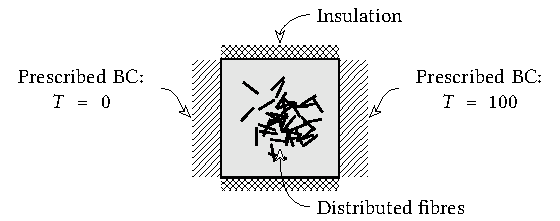
\includegraphics[scale=1]{HC2_RVE_sample.pdf}
\caption{Schematic illustration of the prototype RVE}\label{fig:RVE5}
\end{figure}%

	Dimensionless values were used throughout the investigation, and thus normalized results will be discussed. All the FE models where generated based on a 2D prototype RVE ($10\times10$), which consists of 4-node bilinear isoparametric planar heat transfer elements (type 39) for the matrix phase and straight 2-node link elements (type 36) for fibres, see Fig.~\ref{fig:RVE5}. The contrast of the properties is chosen to be 600, i.e., thermal conductivities of $1$, and $600$ for the matrix and fibres, respectively. An aspect ratio of $40$ was acquired for the fibres, i.e., a fibre length of $5$ and a diameter of $0.125$, to stay within the range of $20$\thinspace--\thinspace$60$ aspect ratios of the short fibres~\autocite{Kalpakjian.2010}.
	
	Considering the effectiveness of boundary conditions~\autocite{Javanbakht.2017b}, the recommended prescribed temperature boundary condition is used~\autocite{Islam.1999}. A temperature gradient of 100 is imposed to set up a steady-state flux across the RVE, see Fig.~\ref{fig:RVE5}. After steady state heat transfer analyses, the reaction flux is collected from the right-hand boundary nodes and summed up to obtain the total heat flux~\autocite{Rakovsky.2014}. Then, the effective thermal conductivity of the RVE is calculated using Fourier's law~\autocite{Fiedler.2009}:
	\begin{equation}
	k_{\text{eff}}=\frac{\dot{Q}}{A_0}\cdot\frac{\mupDelta z}{\mupDelta T},
	\end{equation}%
	where $k_{\text{eff}}$ is the effective thermal conductivity of the RVE, $\dot{Q}$ is the sum of the generated reaction fluxes on the right-hand boundary, $A_0$ is the assumed cross-sectional area (with a thickness of unit length) perpendicular to direction of the flux, $\mupDelta z$ is the distance between the edges of the sample, and $\mupDelta T$ is the prescribed temperature gradient.

Note that a mesh sensitivity analysis was carried out to remove the mesh dependency of the values of effective thermal conductivity. It was carried out over a range of uniform mesh densities ($\gamma$) from 1 to 35~\autocite{Javanbakht.2018}:
\begin{equation}
\gamma=\frac{1}{\ell_\text{mesh}},
\end{equation}
where $\ell_\text{mesh}$ was the edge length of the used square elements. The results showed that the mesh sensitivity was diminished for $\gamma$ over 20 and thus, it was selected as the prototype mesh density for all the simulations.

	The following assumptions are made for creating all the models:
	\begin{itemize}
		\item The thermal conductivity is independent of the temperature.
		\item The transverse conductivity of the fibres is negligible.
		\item A perfect bonding exists between the fibres and matrix, i.e., the thermal barrier resistance is disregarded.
		\item In generating the distributions, overlapping of the fibres is ignored since no explicit cross-section is considered for fibre elements.
	\end{itemize}
	The RVE is divided into four equal partitions which incorporated fibres with equal volume fractions. The locations of the fibres are selected randomly and their orientation followed a von Mises distribution~\autocite{Mardia.1975}. The mean value of the distribution was kept to $\mu=0$ so the fibres are oriented along the direction of the heat flow, see Fig.~\ref{fig:case5}. However, in order to investigate the effect of orientation distribution, the concentration parameter ($\kappa$) was modified from 0 to 50 in the two rightmost partitions to consider the random and highly oriented cases, respectively. 
\begin{figure}[!h]
\centering
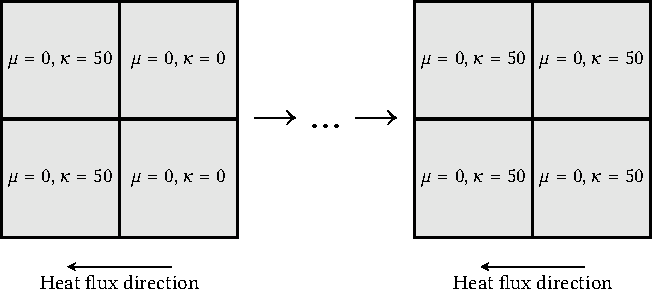
\includegraphics[scale=1]{hc2_RVE}
\caption{Two extreme cases of fibre distribution in the RVE---the fibre volume fraction is kept the same in each partition}\label{fig:case5}
\end{figure}%

\red
	\paragraph{Model validation} In Chapter~\ref{chap:p4}, the results in~\autocite{Fu.2003,Choy.1994} were used to validate the computational model. It was shown that the Hatta-Taya model~\autocite{Hatta.1986,Taya.1989} provided a good agreement with the results. Therefore, the Hatta-Taya model was used to benchmark the FE prototype. The 2D prototype is analysed with the same aforementioned parameters. However since the von Mises distribution was used for planar distribution of fibres, an extreme value for concentration parameter ($\kappa=800$) was chosen to simulate the aligned fibre distribution. 
		
	The response of the FE prototype for aligned short fibres along with the values of the Hatta-Taya model are depicted in Fig.~\ref{fig:hc2_val}. It can be seen that the current model shows a good correlation with the Hatta-Taya model for a wide range of fibre volume fractions. At higher fractions of fibres, the computational model underestimates the effective thermal conductivity.
\begin{figure}[!h]{}
  \centering
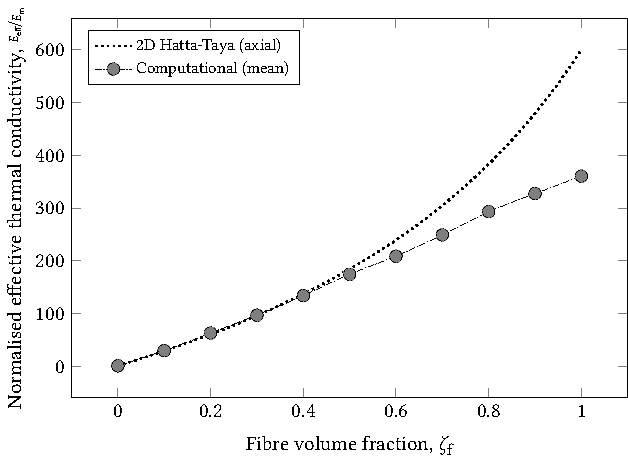
\includegraphics[scale=0.9]{hc2_validation}
  \caption{Validation of the model with the results provided in~\autocite{Fu.2003,Choy.1994}}
  \label{fig:hc2_val}
\end{figure}	
 	In Table~\ref{table:hc2_validation}, the percentage relative error of the computational model with respect to the axial thermal conductivity of the Hatta-Taya model is presented. The computational results show a very good agreement with the benchmark analytical model up to 50\% fibre volume fraction; the percentage relative error remains below 5\%. For higher fibre volume fractions, the model underestimates the thermal conductivity. The maximum error of 40\% is obtained for 100\% fibre volume. Nevertheless, the FE prototype in the current study is used to simulate a low fibre volume fraction of 10\%, and thus can be used confidently.
		
\begin{table}[!h]
\centering
\caption{Effective thermal conductivity results of the computational model against results of the Hatta-Taya micromechanical model.}\label{table:hc2_validation}
\small
\begin{tabular}{*{3}{P{0.07\textwidth}}P{0.1\textwidth}}
\toprule
  $\zeta_{\text{f}}$ \bfs{(\%)}
& {$\frac{k_\text{axial}}{k_\text{m}}$} 
& {$\frac{k_\text{comp}}{k_\text{m}}$} 
& $e_\text{comp}$ \bfs{(\%)}
\\
\toprule
0.10&28.98 & 29.63&-2.22\\
0.20&60.49& 63.16&-4.42\\
0.30&96.22& 96.96&-0.76\\
0.40&137.10& 133.94& 2.31\\
0.50&184.33& 174.55& 5.30\\
0.60&239.49& 208.86&12.79\\
0.70&304.79& 249.09&18.27\\
0.80&383.30& 293.17&23.51\\
0.90&479.46& 327.49&31.70\\
1   &600& 360.58&39.90\\
 \bottomrule
\end{tabular}
\end{table}	

\bl
Finally, a statistical analysis was carried out for each sample by dividing the RVE into four equal partitions. The orientation tensors of the fibres were obtained along with their principal values and directions in each partition and the whole RVE. Finally, the clustering index was calculated for the RVE and correlated with the values of the effective thermal conductivity.  

%TODO would it help to descretize the fibre elements as well?
% ──────────────────────────────────────────────────────────────────────────────────────────────────
\section{Results and Discussion}
	The main focus of the current study was on randomly-oriented fibres, and thus the selection of a pseudo-random algorithm will highly affect the result of the study. Therefore, a von Mises distribution was considered for the orientations to obtain a more controllable approach. In order to challenge the validity of the clustering index, the two rightmost partitions underwent a transition from a random orientation state ($\kappa=0$) to a more concentrated state ($\kappa=50$). This parameter change was applied to fibre volume fractions above the non-dilute limit, i.e., volume fractions from 10\,--\,40\%. The effective thermal conductivity was also calculated in each case and normalized with respect to the thermal conductivity of the matrix.

	Increasing the fibre volume fraction increased the effective thermal conductivity of the composite, see Fig.~\ref{fig:cond5}. Increasing the concentration parameter of the von Mises distribution located more fibres about the flow direction, and thus the thermal conductivity increases. Although the orientation of fibres highly affected the thermal conductivity, this effect seemed to diminish in concentration parameters of more than $\kappa=20$. Furthermore, the effective thermal conductivities showed a lower standard deviation at higher concentration parameters, which is highly noted in lower fibre volume fractions. Namely, by increasing the concentration parameter, more consistent thermal conductivity values were obtained especially for low fibre volume fractions; the latter behaviour can be attributed to the decrease of randomness at low volume fractions.

\begin{figure}[!h]
  \centering
	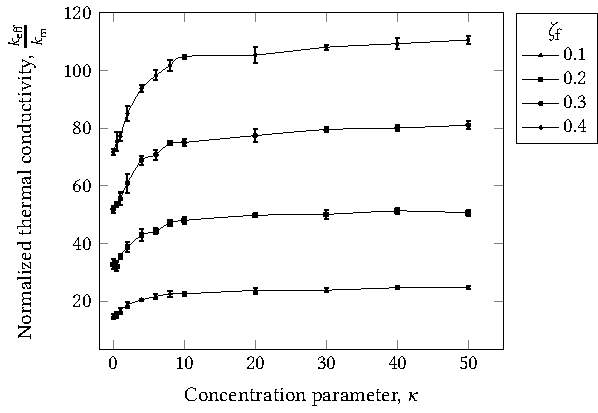
\includegraphics[scale=0.9]{hc2_conduc}
  \caption{Normalized effective thermal conductivity for different concentration parameters and volume fractions}
  \label{fig:cond5}
\end{figure}%

Detection of clustering was investigated using the clustering index obtained from the mixing analogy~\autocite{Ranganathan.1990}. In the case of clustering, it was assumed that a preferred orientation existed along which fibres locally co-orient themselves. The clustering index varies between 0 and 1 where the former indicates a cluster-free state and the latter indicates a clustered state.

The $H_{11}$ component indicates the strength of fibre alignment along the direction of the heat flux whereas the $H_{12}$ component quantifies the dissimilarity in the principal directions of orientation in the partitions of the RVE. The clustering index for component 11 and 12 of the orientation tensor is illustrated in Figs.~\ref{fig:ci11} and \ref{fig:ci12}, respectively. A clustered state was detected for the $H_{11}$ component at the low values of the concentration parameter whereas no clustering was found for the $H_{12}$ component. In addition, a higher standard deviation was observed for the low concentration parameter region, i.e., $\kappa$ less than 20. 

	\begin{figure}[!h]
	\centering
	\subfloat[Clustering index 11 for different concentrations and volume fractions\label{fig:ci11}]{	\includegraphics[scale=0.8]{hc2_c11}}\hfill
	\subfloat[Clustering index 12 for different concentrations and volume fractions\label{fig:ci12}]{	\includegraphics[scale=0.8]{hc2_c12}}
	\caption{Clustering indices of the analysis}\label{figure:hc2_clus}
	\end{figure}%

	Although modest values was generally obtained for the clustering index $[CI]_{11}$, clustering (if any existed) seemed to fade at higher concentration parameters. By increasing the concentration parameter, the clustering state for $H_{11}$ weakened and became negligible for concentration parameters more than 30. Note that no interesting change was observed for the other index, i.e., it indicated a more or less similar principal direction in all cases, see Fig.~\ref{fig:theta}. Namely, no strong orientation tendency was detected. More importantly, no remarkable change was detected by increasing the volume fraction. Thus, one could argue that the orientation tensor is not affected by the fibre volume fraction in the case of uniform distribution of fibre volume. The maximum principal value of the orientation tensor approached to unity by increasing the concentration parameter, see Fig.~\ref{fig:lambdamax}. Namely, orientation of the fibres can be enforced along the flow direction by increasing the greatest eigenvalue---provided that the principal direction remains the same.

\begin{figure}[!h]
	\centering
	\subfloat[Rotation to principal direction with respect to the 1-direction\label{fig:theta}]{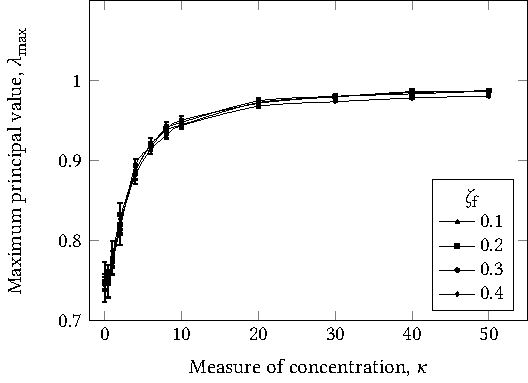
\includegraphics[scale=0.8]{hc2_lambda}}\hfill
	\subfloat[Maximum principal value of the orientation tensor for different concentrations and volume fractions\label{fig:lambdamax}]{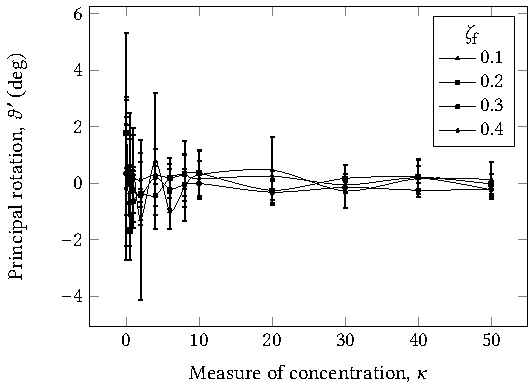
\includegraphics[scale=0.8]{hc2_theta}}
	\caption{Results of spectral analysis}\label{fig:hc2_spectral}
\end{figure}


\section{Conclusion}
\red
	The current study attempted to relate the effect of fibre clustering and effective properties of an RVE. It was observed that by increasing the concentration parameter, the strength of clustering decreases while the orientation clustering remains unaltered.\bl~It can be concluded that increasing the fibre volume fraction increases the effective thermal conductivity of the composite. This is highly effected by the orientation state of the fibres, i.e., a clustered fibre distribution may inhibit the heat flux. Moreover, orienting the fibres along the heat flow facilitates heat transfer---provided that clustering is minimum. This is true specially when the principal direction of the fibres remains along the heat flow and the clustering index does not change along this direction. Finally, by increasing the maximum principal value of the orientation tensor, alignment of the fibres can be further enforced along the flow direction which results in an efficient use of fibres for improving thermal conductivity. This approach can be used to characterize the composite and determine its degree of efficiency in terms of fibre engagement both in thermal in mechanical aspects of a composite.

    % !TeX spellcheck = en_GB
%!TEX TS-program = xelatex
%!BIB TS-program = biber

\chapter{Modelling Natural~Fibre Composites Using Strength-updating}\label{chap:p6}
\section*{Statement of Contribution}
\vspace{-0.5\baselineskip}
	This chapter includes a co-authored journal paper. The bibliographic details of the under review paper are:
\begin{itemize}
	\item Javanbakht, Z, Hall, W, Virk, Amandeep Singh, Summerscales, John \& Öchsner, A (2019), ``Finite Element Analysis of Natural Fibre Compolsites Using a Self-Updating Model'', Journal of Composite Materials, accepted.
\end{itemize}
	My contribution as the corresponding author to the paper involved: undertaking literature review, classifying the necessary theoretical backgrounds and models, developing the programming code, analysing and discussing the finite element results, drawing figures, preparing tables, writing and editing the manuscript according to my supervisors’ comments. The experimental values were provided by Dr Amandeep Singh Virk, Associate Professor Wayne Hall, and Professor John Summerscales.
	

\Zia\\
\Wayne
\vfill
\pagebreak

% --------------------------------------------------------------------------------------------------

\paragraph{Title} Finite Element Analysis of Natural Fibre Composites Using a Self-Updating Model

\paragraph{Abstract} The aim of current work was to illustrate the effect of the fibre area correction factor on the results of modelling natural fibre reinforced composites. A mesoscopic approach is adopted to represent the stochastic heterogeneity of the composite, i.e., a meso-structural numerical model was prototyped using the finite element method including quasi-unidirectional discrete fibre elements embedded in a matrix. The model was verified by the experimental results from previous work. A correction factor was suggested to fine-tune both the analytical and numerical models. Moreover, a model updating technique for considering the size-effect of fibres is introduced and its implementation was automated by means of FORTRAN subroutines and Python scripts. It was shown that correcting and updating the fibre strength was critical to obtain accurate macroscopic response of the composite when discrete modelling of fibres is intended. Based on the findings of the current study, considering the effect of flaws on the strength of natural fibres and the fibre area correction factor are crucial to obtain realistic results. 

% ══════════════════════════════════════════════════════════════════════════════════════════════════
\section{Introduction}
	% Importance of natural variability application of natural fibres
	From a structural point of view, natural fibres are available over a range of acceptable mechanical properties. However, taking advantage of natural fibres as structural elements requires embedding them in appropriate matrices. Although the resulting natural fibre composites (NFCs) would have enhanced specific properties, the variability of the fibre properties remains inherent. This argument is confirmed by the wide range of reported values.~\autocite{Pickering.2016} Thus, in order to properly characterise NFCs, various sources of variability must be taken into account.
	
	% What are the natural variations that affect material properties? Why CSA measurement is important?
	Natural variation is not only source-dependent but also occurs within a single batch of fibres, e.g., cross-section non-uniformity~\autocite{AlvesFidelis.2013}, length-dependent strength~\autocite{Virk.2013b}, moisture content~\autocite{Javanbakht.2017b}, and void content~\autocite{Senthilkumar.2018} among others affect the mechanical properties of fibres. Moreover, such parameters can substantially interfere with the characterisation process of some properties. Irrespective of the level of sophistication, providing a universal model is not feasible, and thus one should be selective. In terms of the mentioned parameters, the first two sources of variation are `structural' ones, which are the results of the growth period of natural fibres. The moisture content is affected by the environment, and thus it is disregarded in the study. Finally, the void content becomes \textit{more} relevant when moisture is investigated. Therefore, the first two aspects are revisited herein.
	
	Of our particular interest is the morphology of the fibres that affect their cross-sectional area (CSA) measurements, and thus the strength calculations. The cross-sectional shape varies along the length and from one fibre to another.~\autocite{Virk.2010b} This shape irregularity gives rise to two new concepts: the `true' cross-sectional area and the `measured' or `apparent' one. Values of the former deviate from those of the latter. This discrepancy is traced back to a simplistic assumption, which is clarified in the sequel, during the CSA measurement.
	
	The `apparent' fibre CSA is often incorrectly measured and used. Apparent CSA is calculated from an average of several linear measurements of fibre diameter (assuming a circular cross-section). This method can result in significant variation in mechanical properties due to the assumption that the ``non-circular fibres have a characteristic diameter''.~\autocite{Virk.2013} More specifically, the measured CSA is an overestimation of the real CSA. This discrepancy demands corrections in the analytical models as well as the computational ones.

	From the fracture mechanical point of view, the strength size effect of structural elements should be considered in design processes.~\autocite{Bazant.2000} Natural fibres are not exceptions to this matter. Virk et al.~\autocite{Virk.2013b} experimentally measured the tensile properties of 500 jute fibres from a single batch in five gauge lengths. Weibull theory and the weakest-link model were used to capture the statistical size effect of the single fibre response under tension. It was found that although the elastic modulus of fibres remains insensitive to length, their ultimate tensile strength decreases by increasing the fibre length.
		
	% why analytical values are useful
	Using analytical models, such as various forms of rule of mixture (RoM), is an elegant attempt to predict the mechanical properties of NFCs. The major drawback of such models is that they do not often incorporate all the microstructural parameters such as clustering of the fibres. Attempts have been made to relate the manufacturing processes to the resulting microstructure, and thus the properties of the composite.~\autocite{Summerscales.2017} Often such attempts include developing a statistical model to improve the predictions. For instance, orientation distribution functions could be derived for a specific sample (by means of methods like image processing) although the cumbersome process lacks generality. In any case, analytical models provide a good range for the expected values in general. Nevertheless, various correction factors have been suggested to compensate for the lack of microstructural considerations and further refine the limits provided by the analytical estimates.~\autocite{Summerscales.2013}
	
	% the importance of computational models
	In the next level, computational models can be set up in a way that---after validation and verification---extension to arbitrary (or even physically-impossible) cases would be possible. The accuracy of such models depends on the precision of the input data (e.g., material properties of the components and the geometry of constituents) as well as the intricacy of the  modelling strategies and techniques (e.g., multi-scale and average-field methods). In addition, the trade-off between computational resources and accuracy is always present. For instance, instead of modelling the actual structure, a representative volume element (RVE) might be used. Nevertheless, real-size computational models with adequate refinements are expected to be the closest representation of the their physical counterparts. Herein, the finite element (FE) analysis~\autocite{Oechsner.2016,Javanbakht.2018} is used for its widespread availability.
	
	% Aim
	The aim of the current study is to provide a computational framework for modelling discrete embedded fibre elements in NFCs considering the aforementioned parameters: correction of the CSA and size-dependency of fibre strength. In the following sections, some analytical models are introduced that are followed by a computational model. The details of the FE prototype is explained and its response is validated against experimental data. The accuracy of the results generated by two algorithms is compared against analytical boundaries. Finally, further suggestions are made for future developments.%Then, a parametric study is carried out to test the hypothesis that the increase of fibre volume fraction will alter the results of the models or not. 
	
\section{Enhanced Rule of Mixture}
	The classic homogenisation formulas for unidirectional composites, i.e., the RoM and the inverse rule of mixture (IRoM), are based on the iso-strain and iso-stress assumptions, respectively:
	\begin{subequations}
	\begin{alignat}{2}
		E_\parallel 		=& \zeta_\text{f}E_\text{f}          &&+\zeta_\text{m}E_\text{m},\\
		\frac{1}{E_\perp}	=& \frac{\zeta_\text{f}}{E_\text{f}} &&+ \frac{\zeta_\text{m}}{E_\text{m}},
	\end{alignat}
	\end{subequations}
	where $\zeta$ is the volume fraction and $E$ is the elastic modulus. The subscripts `$\text{f}$' and `$\text{m}$' are used to denote the properties related to the fibres and the matrix, respectively. The elastic moduli $E_\parallel$ and $E_\perp$ are estimates in the longitudinal and transverse directions, respectively. Several theories modified these formulas, specially the RoM, by fine-tuning the contribution of fibres via an efficiency parameter. Inspired from the enhanced version of the generalised RoM, the fibre efficiency parameter~\autocite{Summerscales.2019} ($\varkappa$) is reintroduced as:
	\begin{equation}
		\varkappa \equidef \varkappa_\text{a}\varkappa_\text{d}\varkappa_\text{l}\varkappa_\text{o},\label{eq:kappa}
	\end{equation}
	where $\varkappa_\text{a}$ is the fibre area correction factor (FACF), $\varkappa_\text{d}$ is the fibre diameter distribution factor (FDDF), $\varkappa_\text{l}$ is the fibre length distribution factor (FLDF), and $\varkappa_\text{o}$ is the fibre orientation distribution factor (FODF), respectively.
	
	The FLDF can be obtained from the traditional Shear-Lag model~\autocite{Cox.1952} or the generalised version~\autocite{Nairn.2004}. The FODF is calculated by~\autocite{Krenchel.1964}
	\begin{equation}
		\eta_\text{o}=\sum_n a_n\cos^4\theta,\label{eq:krenchel}
	\end{equation}
	where $a_n$ is the fraction of fibres making a $\theta$ angle with the direction of the applied load. If the angle distribution follows a probability distribution function (PDF), $a_n$ can be calculated directly. For instance in the case of a normal distribution, the FODF reads
	\begin{equation}
		\varkappa_\text{o}=\int_{-90}^{90}\frac{1}{\sigma_\text{N}\sqrt{2\pi}} \exp\left(-\frac{(\theta-\mu_\text{N})^2}{2\sigma_\text{N}^2}\right)\cos^4\theta\,\dif\theta,
   	\end{equation}
	where $\mu_\text{N}$ and $\sigma_\text{N}$ are the mean and standard deviation of the normal distribution, respectively. Alternatively, the overall fibre orientation can be captured by even-order orientation tensors from which the PDF of the orientation can be estimated, see~\autocite{Javanbakht.2019,Javanbakht.2017c,Advani.1987}.
	
	Finally, the enhanced rule of mixture (En-RoM) is~\autocite{Summerscales.2013} 
	\begin{equation}
		E = \varkappa \zeta_\text{f}E_\text{f}+\zeta_\text{m}E_\text{m},\label{eq:enrom}
	\end{equation}
	where $E$ is the elastic modulus of the composite along the applied load---since FODF is calculated by Eq.~\eqref{eq:krenchel}. Moreover, a homogeneous behaviour is assumed to be dominant, i.e., other local variabilities such as resin-rich areas, porosities, or fibre clustering are neglected implying a smeared response. Note that the overall effect of the aforementioned correction factors reduces to unity under specific conditions, i.e., for continuous fibres FLDF, and for well-characterised circular cross-section fibres the FDDF and FACF become unity. Namely, RoM can be considered as a special case of the En-RoM.
	
	The FACF is suggested by Virk et al.~\autocite{Virk.2009} to compensate for the deviation between the apparent and true fibre CSAs. A typical value of 1.42 was initially suggested for the specific batch of tested jutes fibres. Similarly, extending the Kelly-Tyson model~\autocite{Kelly.1965} enables calculating the strength of a unidirectional composite $\sigma^\prime$ by means of an enhanced Kelly-Tyson model (En-KT):
	\begin{equation}
		\sigma^\prime = \kappa \zeta_\text{f}\sigma^\prime_\text{f}+\zeta_\text{m}\sigma^*_\text{m},\label{eq:en-KT}
	\end{equation}
	where $\sigma^\prime_\text{f}$ is the strength of fibre, and $\sigma^*_\text{m}$ is the stress in the matrix at composite failure. Note that this equation is only applicable to matrices with a higher failure strain than that of the used fibres.

\section{Weibull Distribution}
	In order to capture a better image of a random variable, a statistical evaluation is used to obtain its distribution. Weibull distribution is a generalisation to exponential distribution, and thus the normal distribution can also be considered as a special case thereof. The three-parameter Weibull distribution is the most general case for which the probability distribution function (PDF) of a random variable $x$ is stated as
    \begin{equation}
    	P(x)=\frac{\beta}{\alpha}\left(\frac{x-\gamma}{\alpha}\right)^{\beta-1}e^{-\left(\frac{x-\gamma}{\alpha}\right)^\beta},
    \end{equation}
    where $\alpha$ is the scaling (characteristic) parameter, $\beta$ is the shape parameter, and $\gamma$ is the location parameter. The mean value of the Weibull distribution ($\bar{x}$) is obtained from:
    \begin{equation}
       	\bar{x}=\gamma +\alpha \Gamma\left(\frac{1}{\beta}+1\right), \label{eq:strength}
    \end{equation}
    where the gamma function $\Gamma(z)=\int_{0}^{\inf}x^{z-1}e^{-x}\dif x$ is the generalisation of the factorial from the domain of integers to real numbers.

    Increasing the scaling parameter stretches the distribution horizontally. For a monotonic decrease in distribution, the shape parameter is set between 0 and 1 whereas values more than one indicate an increase followed by a decrease in the PDF. The location parameter just shifts the distribution to the right-hand side, i.e., it acts as a `threshold' below which no random variable $x$ could exist~\autocite{Milton.2003}. Thus, in most practical cases where only positive values are admissible, e.g., strength calculations, $\gamma$ is set to zero; this results in the two-parameter Weibull PDF:
    \begin{equation}
        P(x)=\frac{\beta}{\alpha}\left(\frac{x}{\alpha}\right)^{\beta-1}e^{-\left(\frac{x}{\alpha}\right)^\beta}.
    \end{equation}    
     The obtained strength distribution from~\autocite{Virk.2013b} is based on the average apparent CSA of 785 fibres. For each fibre, three measurements were carried out to capture the CSA variation along the length. Since the measurements overestimated the CSA, they underestimate the material properties, e.g., elastic modulus and strength of the fibre material. This artefact is present in the measurements, and thus propagates to the statistical model. Therefore, to compensate for the CSA miscalculations, Eq.~\eqref{eq:strength} is modified to
    \begin{equation}
       	\bar{x}_\text{mod}=\varkappa_\text{a}\alpha \Gamma\left(\frac{1}{\beta}+1\right).\label{eq:strengthcorrected}
    \end{equation}
	Furthermore, the same correction factor must be applied to the measured elastic modulus.

\section{Computational Model}
	A probabilistic FE prototype has been developed to reproduce the mechanical behaviour of jute-epoxy NFCs. A variety of tools were used along with the semi-open MARC/MENTAT 2019 FE package to avoid developing a programming code from scratch~\autocite{Javanbakht.2017}. The FE model was prototyped by means of a Python~script that automated the process of parametric model generation and controlled the job submissions~\autocite{Javanbakht.2016}. 
	
	
	The interaction of the Python script and FORTRAN subroutines is illustrated in Fig.~\ref{fig:m}. The pre-process was done by means of a Python script that interacted with the MENTAT pre/post processor and later submitted the job to the MARC solver for analysis. Although the FE package was responsible for obtaining the solution, controlling the fibre and matrix failure was carried out by means of several FORTRAN subroutines. Namely, at the end of every increment, the stress of each present fibre was obtained from its integration point and compared with the average strength of the Weibull distribution from Eq.~\eqref{eq:strengthcorrected}. A failure is predicted for stresses above the mean strength and the respective element is removed. Depending on the location of the element, new fibres may be created or the length of the parent fibre decreases. Two approaches are adopted: either update the strength of the fibres or inherit the strength from the parent fibre. Either approach follows the flowchart in Fig.~\ref{fig:m} but in the latter approach, the `update the strength of fibres' step is dropped. For the failure of the matrix element, the maximum stress failure criterion was used to be compared against the average of the stresses obtained from the integration points of the element. The load increments continues until the failure of the sample; convergence failure would flag this state.
	
	\begin{figure}[!t]
	\centering
	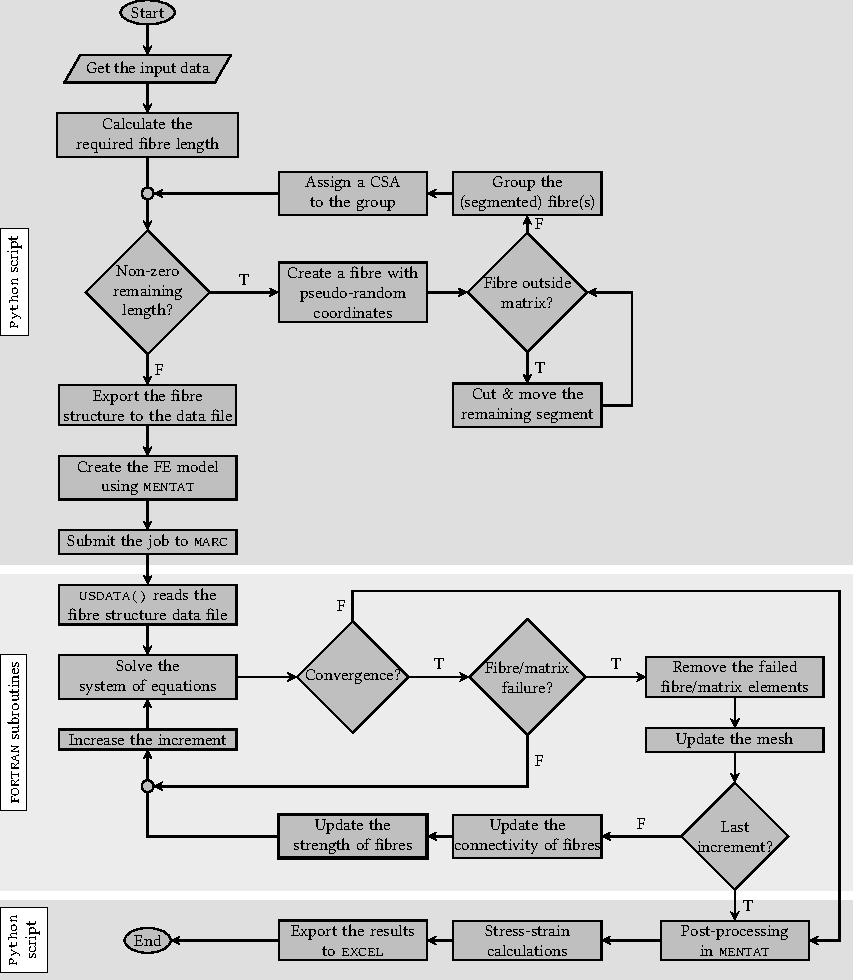
\includegraphics[width=\textwidth]{fig1_flowchart.pdf}
	\caption{Flowchart of the model creation, analysis, and post-process}\label{fig:m}
	\end{figure}
	A uniform mesh density was used throughout the model to facilitate the mesh sensitivity analyses. More specifically, the mesh density~\autocite{Javanbakht.2016b} is defined as
	\begin{equation}
		\gamma\equidef\frac{1}{\ell_\text{mesh}},
	\end{equation}
and controlled to obtain convergence while a single mesh length ($L_\text{mesh}$) is used for both fibre and matrix elements in the FE prototype. The number of elements used to represent each fibre depended on the fibre length, i.e., longer fibres consisted of more elements than shorter fibres in order to comply with a uniform mesh density. To this end, different length fibres were discretised into truss elements of the same size. A typical jute-epoxy FE model is shown in Fig.~\ref{fig:fe} in which the localised fibre/matrix failure region is enlarged.

	\begin{figure}[t!]%TODO add undamaged, damaged w/t and w/o the algorithm figures & write a qualitative (visual) description of the result
		\centering
		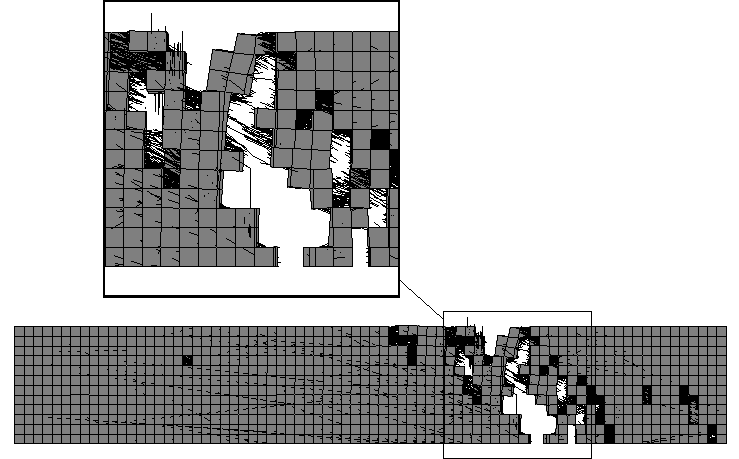
\includegraphics[width=\textwidth]{fig2_tensile_fe.pdf}
		\caption{Finite element model of a jute-epoxy composite sample upon failure (top view)}\label{fig:fe}
	\end{figure}

\subsection{Modelling Fibres}	
	The jute fibres and epoxy matrix were discretely modelled. Each fibre was represented using several simple truss elements (type 9) whilst 3D solid elements (type 7) were used to represent the matrix. The type 9 truss elements were two-node, single integration point elements with three translational degrees of freedom. The solid elements used in the matrix were eight-node isoparametric elements that utilised trilinear interpolation functions equipped with a full integration scheme. 
	
	The jute fibres were modelled as straight fibres with a constant CSA. Namely, technical fibres were modelled as a whole without considering individual elemental fibres, voids, resin impregnated volumes, or other internal structures. However the true shape of the cross-section was taken into consideration by means of the FACF. Since the elements are basically 1D, the Poisson's effect is also ignored.
	
	%TODO add a reference for the wall effect
	The distribution of the fibres satisfied material periodicity in order to avoid any wall effects.~\autocite{Miehe.2002} Although the distribution of fibres was quasi-unidirectional, they were allowed to penetrate through the walls of the matrix (sometimes called a soft boundary). Once a fibre penetrated the edge of the specimen, it was cut from the intersection point and the remaining segment is used to create a new fibre starting from the opposite edge. This arrangement was due to the fact that the tensile specimens were cut from a larger plate during manufacturing, and thus by following the explained procedure, the created samples better represent the parent material.
	
	% Do find references for softening
	Note that a quarter of the tensile specimen was considered instead of the whole specimen to reduce numerical load. Moreover, choosing an RVE was not considered since removing elements has a damage-like effect that results in softening of the response. An RVE---according to the ergodic hypothesis---must represent the whole structure over time. When very localised effects are present, e.g., softening in the form of degradation of elasticity, the RVE cannot present the whole structure that is showing a holistic behaviour. Namely, considering the whole structure is inevitable when various localised effects are present. In the current context, resin-rich areas and fibre clustering could make the unit cell approach not a good representation of the whole structure unless such imperfections are ignored. Finding an appropriate RVE by increasing the size of the realisations encounters convergence problems under softening behaviour and is still under investigation.~\autocite{Gitman.2007} This issue is closely related to the size effect issue that is mentioned in the introduction.
	
	
	The CSA for each fibre was selected from a log-normal distribution of the `true' fibre area~\autocite{Virk.2010b}. The `location' and `scale' parameters of 7.55 and 0.52 were used to characterise the true fibre CSA distribution, respectively. This log-normal distribution offers a realistic fit to the true cross-sectional area measurements of 106 jute fibres that were extracted from the same batch and were used to manufacture the jute-epoxy composite samples. Figure~\ref{fig:fibCSA} illustrates the possible discrepancy if the apparent CSA is used. These measurements were overlaid with the apparent and true log-normal CSA distribution for the jute fibres. 
	\begin{figure}[!t]
		\centering
%		\includegraphics[width=0.45\textwidth]{csa}
		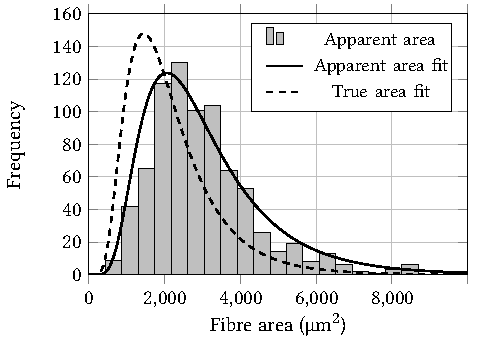
\includegraphics[scale=1]{fig3_area_dist}
		\caption{Fibre cross-sectional area distribution with $\text{FACF}=1.42$ (reproduced from~\autocite{Virk.2013})}\label{fig:fibCSA}
	\end{figure}
	
	The mechanical properties of the jute fibres, represented in the model, are influenced by fibre length~\autocite{Virk.2013, Virk.2009,Virk.2011}. Whilst the elastic modulus for the batch of jute fibres is relatively insensitive to fibre length, fracture strength and strain significantly reduce as fibre length increases~\autocite{Virk.2013b,Virk.2009}. Thus, to account for fibre length variations (and the interrelated mechanical properties), a log-normal distribution of fibre lengths was included with the location and scale parameters of 4.183 and 0.976, respectively. This log-normal distribution is representative of the fibre distribution resulting from 700 jute fibre measurements~\autocite{Virk.2009}. A comparison of the jute fibre length measurements and the log-normal fit (obtained using these location and scale parameters) is shown in Fig.~\ref{fig:len}.%TODO Proof-read until here

	\begin{figure}[!h]
		\centering
%		\includegraphics[width=0.50\textwidth]{len}
		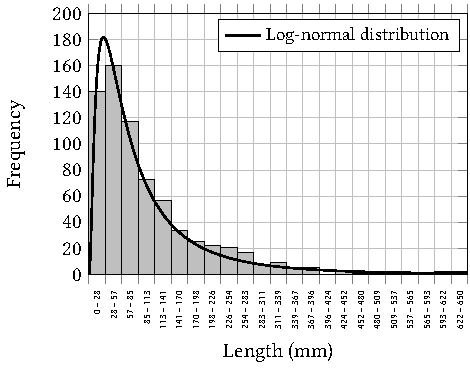
\includegraphics[scale=1]{fig4_len_dist}
		\caption{Fibre length distribution; reproduced from~\autocite{Virk.2009}}\label{fig:len}
	\end{figure}
		
	The elastic modulus of the jute fibres was taken (for each fibre) to be the mean of the 785 jute samples tested. This mean value (27.9\,GPa) is sensibly independent of fibre length~\autocite{Virk.2013}. In contrast, the failure strengths of the fibres were calculated based on fibre length and included in the FE models. The natural logarithmic interpolation model reported in~\autocite{Virk.2011} was used to calculate the fracture strengths for each fibre based on its length. The work of~\autocite{Virk.2011,Virk.2013} assumes a circular fibre cross-section. The elastic modulus and fracture strengths were therefore based on the apparent CSA. Thus, the FACF needed to be applied to both elastic modulus and failure strength of the fibres. A FACF of 1.42~\autocite{Virk.2010b} is included in the FE model for the elastic modulus and failure strength of the fibres as per Eqs.~\eqref{eq:enrom} and \eqref{eq:strengthcorrected}, respectively. Finally, the orientation of the fibres follows a Gaussian distribution, see Table~\ref{table:tests}. In this table, the mechanical properties and geometrical dimensions of five jute fibre reinforced composite samples (cases A--E) are summarised; they correspond to the experimental results in~\autocite{Virk.2013} (see the `Experimental Data' section for more details).

	% TABLE WITH 5 CASES [CASE B is omitted]
	\begin{table}[!th]
	\centering\small
	\caption{Measured mechanical properties of jute-epoxy composite (Plate values are the average values of the samples). Adapted from~\autocite{Virk.2013}.}\label{table:tests} 
	\begin{tabular}{lccccccc@{ }cc }% *{8}{>{\hfill}c}}
	\toprule
	\multicolumn{2}{l}{\multirow{2}{*}{\bfs{Property}}}&	
	\multicolumn{4}{c}{\bfs{Sample}}&
	&&\multicolumn{2}{c}{\bfs{Plate}}\\\cmidrule{9-10}\cmidrule{3-7}
	&&{\bfs{A}}	
	& {\bfs{B}}
	& {\bfs{C}}
	& {\bfs{D}}
	& {\bfs{E}}
	&&\bfs{Mean}	&\bfs{SD}\\
	\toprule
	\multicolumn{2}{l}{Width (mm)}		  				&25.14	&25.02	&25.06	&24.87	&25.03	&&25.05	&0.09\\
	\multicolumn{2}{l}{Thickness (mm)}					&3.15	&3.61	&3.67	&3.59	&3.67	&&3.52	&0.18\\
	\midrule
%	\multicolumn{2}{l}{Elastic modulus (GPa)}   		&8.98	&8.28	&7.79	&7.33	&8.70	&8.19	&0.55\\
%	\multicolumn{2}{l}{Tensile strength (MPa)}			&104.90	&99.60	&106.80	&94.80	&94.20	&100.06	&5.12\\
%	\multicolumn{2}{l}{Failure strain (\%)}				&1.26	&1.29	&1.40	&1.41	&1.15	&1.30	&0.10\\
	%\multicolumn{2}{l}{Poisson's ratio (longitudinal)}	&0.42	&0.42	&-		&0.44	&-		&0.42	&0.01\\\hline
	\multirow{2}{*}{Volume fraction (\%)}	&\ Mean		&17.50	&20.30	&20.90	&18.00	&18.50	&&18.88	&1.483\\
											& SD		&3.20	&3.80	&6.10	&3.10	&5.40	&&3.95	&n/a\\\midrule
	\multirow{2}{*}{Fibre angle ($^\circ$)}		&Mean	&5.72	&10.52	&7.90	&6.19	&6.59	&&7.36	&1.932\\
											&SD			&15.32	&18.44	&15.05	&16.09	&15.59	&&17.95	&n/a\\\midrule
	\multicolumn{2}{l}{$\eta_\text{o}$}					&0.86	&0.77	&0.85	&0.85	&0.85	&&0.81	&0.06\\
	\multicolumn{2}{l}{$\kappa$}			                        & 1.42&1.42&1.42&1.42&1.42&&1.42&0.00\\
	\multicolumn{2}{l}{$\eta_\text{d}$ or $\eta_\text{l}$}			& 1.00& 1.00& 1.00& 1.00& 1.00&&1.00&0.00\\
		\bottomrule
	\end{tabular}
	\end{table}

\subsection{Modelling the Matrix}
   	The fibres are modelled by means of two-node rod elements with linear shape functions. They are inserted into the matrix elements in a way that the degrees of freedom (DoFs) of the embedded elements take their values from those of the host (matrix) elements. The DoF values are interpolated based on the isoparametric location of the embedded node within the host. The mesh density of the matrix elements followed that of the fibres to facilitate the fibre embedding process ($\lambda=1$).
   	
   	Since the volume of the fibre elements is overlapped with that of the matrix elements, the volume of the matrix is artificially increased. Thus, a `virtual' thickness must be used instead of the real (original) thickness of the matrix:
   	\begin{equation}
   		t_\text{m,v}=(1-\zeta_\text{f})t_\text{m},
   	\end{equation}
   	where $t_\text{m}$ is the original matrix thickness and $t_\text{m,v}$ is the virtually decreased matrix thickness. Note that the volume fraction calculation is done with respect to the original thickness. A summary of the used properties is listed in Table~\ref{table:mech_p}. 
	
	\begin{table}[!b]
	\centering\small
	\caption{Summary of material properties}\label{table:mech_p}
	\begin{tabular}{p{0.1\textwidth}p{0.31\textwidth}p{0.5\textwidth}}
	\toprule
	\bfs{Material} 	& \bfs{Parameter} 	& \bfs{Value}\\
	\toprule
	Jute fibre		& Constitutive law				& Linear elastic, isotropic\\
					& Axial elastic modulus				& $27.9$ GPa~\autocite{Virk.2013} \\
					& Axial-radial Poisson's ratio				& $0.35$~\autocite{Virk.2016} \\
					& Failure criterion				& Maximum normal stress \\
					& Failure strength distribution	& Logarithmic interpolated Weibull distribution~\autocite{Virk.2011}\\
					& Characteristic strength&$\alpha_\text{log}=-111.656\ln(L_\text{fibre})+801.63$\, MPa\\ 
					& Shape parameter&$\beta_\text{log}=-0.152\ln(L_\text{fibre})+3.487$\\
					& Average axial fibre strength$^\dagger$ & $298.13\,\text{MPa}$\\
					& Fibre length distribution			& Log-normal ($\text{mean}=4.183$, $\text{SD}=0.976$)\\%(mean=65.6, STD=2.65)\\
					& CSA distribution				& Log-normal ($\text{mean}=7.55$, $\text{SD}=0.52$)\\%(mean=1900.74, STD=1.682)\\
					& Orientation distribution		& Gaussian ($\text{mean}=5$, $\text{SD}=10$) \\
					& Mean fibre orientation factor & $0.81\pm0.06$\\\midrule
	Epoxy			& Constitutive law				& Linear elastic, isotropic\\
					& Elastic modulus				& $2.65\,\text{GPa}$~\autocite{Virk.2013} \\
					& Poisson's ratio				& $0.35$~\autocite{Virk.2016} \\
					& Failure criterion				& Maximum normal stress\\
					& Failure strength				& $61\,\text{MPa}$~\autocite{Virk.2013}\\
					& Failure strain (\%)			& $4.1$~\autocite{Virk.2013}\\\midrule
	\multicolumn{3}{l}{$^\dagger$ The average axial strength corresponds to a fibre with average length in the distribution.}\\\bottomrule
	\end{tabular}
	\end{table}

%TODO back up using the max. shear stress critera by literature, READ the book that presented this
%TODO where exactly the FACF is applied in the model?

\subsection{Experimental Data}

	% description of experiments
	Experimental results in~\autocite{Virk.2013} were used as benchmark values. Five samples from a single jute fibre reinforced composite plate were cut, measured and prepared (five cases A--E). Micrographs (6--8 per sample) were taken to characterise the micro-structure of the samples, i.e., to estimate their volume fraction and the fibre orientation PDF by means of an image processing procedure. The statistical results were used to calculate the FODF and FACF for each sample. Since the diameter of the fibres were characterised accurately, a unit value was assigned to the fibre diameter distribution factor. In addition, the fibre length distribution factor was assumed to be equal to 1. The experimental results are summarised in Table~\ref{table:results}.



	% creating the validation models
	To account for the stochastic variations in fibre CSA, length and mechanical properties, as well as to accommodate the possible deviations in fibre orientation for the jute-epoxy composite samples, five pseudo-random realisations of the prototype were developed per case.  In each realisation, quasi-unidirectional fibres with variable length and CSAs were dispersed in a 3D matrix as per the distributions of Tables~\ref{table:tests} and~\ref{table:mech_p}. Moreover, each realisation was analysed twice: with updating the strength of the fibres and without strength updating. The simulations were carried out for jute fibre-reinforced composite samples with low fibre volume fractions (in the range 17.5--20.9 vol\%). A total of 50 probabilistic FE models were therefore considered. The stress-strain curve for one of the realisations of Case D is depicted in Fig.~\ref{fig:stressstrain}.

	\begin{figure}[!t]
		\centering
		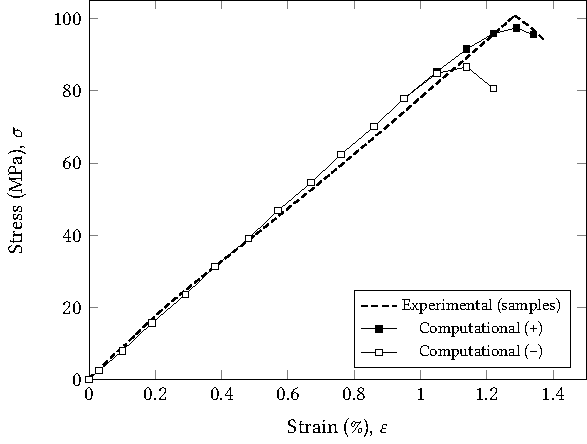
\includegraphics[scale=1]{fig5_fea_vs_test.pdf}
		\caption{Stress-strain response for a single realisation of Case D with $V_\text{f}=18\%$ (the $+$ and $-$ symbols denote the `with strength updating' and `without strength updating' algorithms, respectively)}\label{fig:stressstrain}
	\end{figure}%
In summary, in order to have a model that statistically represent the real specimens, the computer-generated prototype provides the following capabilities:
\begin{itemize}
\item discrete modelling of embedded fibres;
\item generating arbitrary volume fractions;
\item controlling various statistical features, e.g., the length, CSA, strength, and the orientation distribution of the fibres;
\item generating and updating length-dependent strength according to the Weibull distribution; 
\item applying the relevant correction factors to the material properties, e.g., FACF to natural fibres; 
\item applying the volumetric correction factor (by means of a virtual thickness) to compensate for the volume of the embedded fibres in the matrix; and
\item applying element elimination technique to both matrix and fibre elements based on the maximum stress failure criterion (implementing other criteria is also possible).
\end{itemize}
	

\section{Results and Discussion}
	A total of 25 realisations were analysed; first with updating the strength of fibres, and then without this consideration. The simulations were carried out according to the statistical results obtained from experiments, i.e., the same volume fractions, fibre angle orientation distributions, fibre CSA distributions, and fibre length distributions were used. Elastic modulus, tensile strength, and failure strain of the simulations were calculated and illustrated in Fig.~\ref{fig:main_results}. The values and their corresponding percentage relative differences are available in Table~\ref{table:results}. Obviously, the obtained values are bound to the limitations of pseudo-random model generation. Nevertheless, some useful derivations are obtained by analysing them.

	
\begin{figure}[!t]{}
  	\centering
  	\subfloat[][Elastic moduli\label{fig:E}]{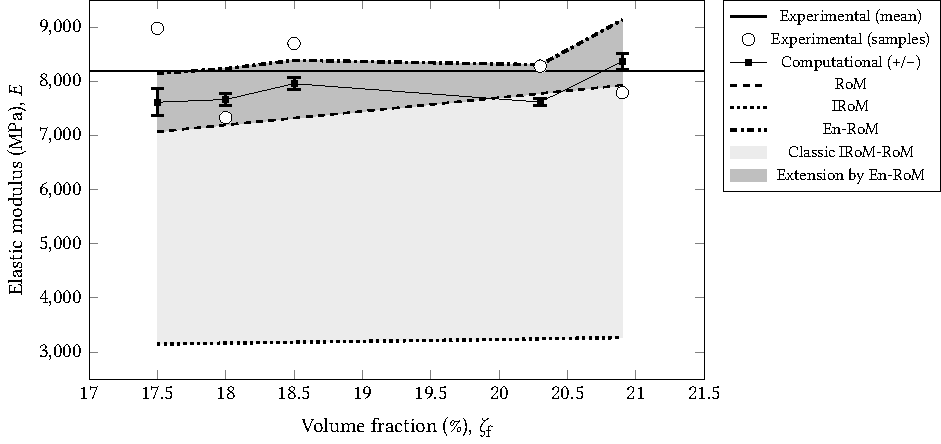
\includegraphics[height=0.28\textheight]{fig6a_E}}\\
  	\subfloat[][Tensile strength\label{fig:stress}]{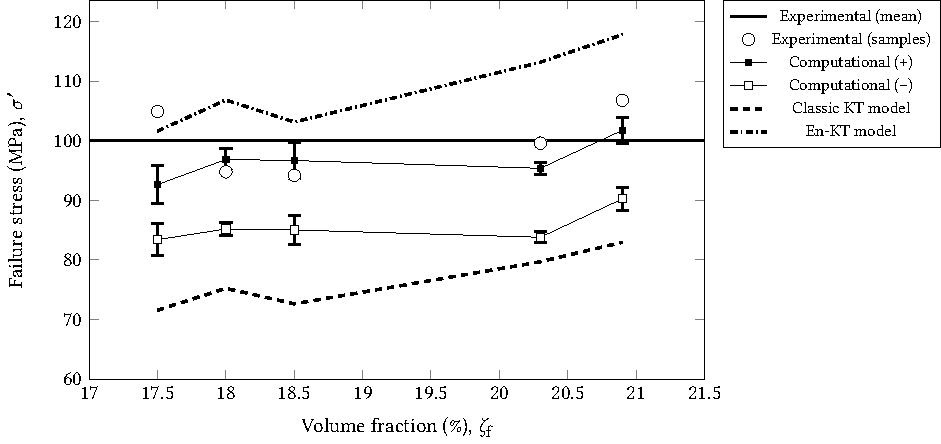
\includegraphics[height=0.28\textheight]{fig6b_strength}}\\
 	\subfloat[][Failure strain\label{fig:strain}]{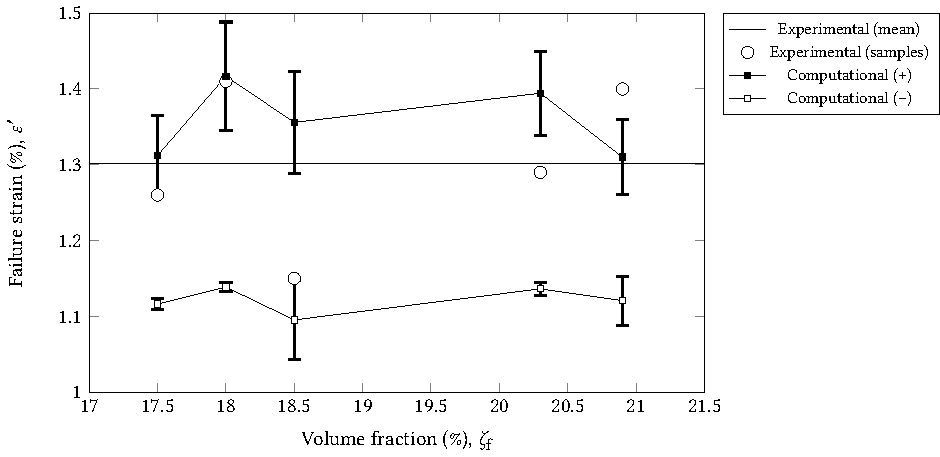
\includegraphics[height=0.28\textheight]{fig6c_failure_strain}}\\
	\caption{Results of experimental, computational, and analytical models (the $+$ and $-$ symbols denote the `with strength updating' and `without strength updating' algorithms, respectively).}
	\label{fig:main_results}
\end{figure}%
\afterpage{\clearpage}


	\paragraph{Elastic modulus} The experimental values for the elastic moduli were outside the range predicted by the classic IRoM and RoM, see the lightly shaded region in Fig.~\ref{fig:E}. The estimated upper value by RoM is extended by means of the En-RoM according to Eq.~\eqref{eq:enrom}; the extended region is shaded slightly darker in the figure. Moreover the averaged value of the specimens---the black horizontal line that corresponds to the plate value---resides mostly in the area that is extended by the En-RoM. The elastic moduli obtained from the numerical analyses were insensitive to updating the strength of the fibres as both computational values overlap. Similar to the experimental results, the computational values are mostly in the extended region. If the plate value is taken as the representative of the material, the computational approach seems to slightly underestimate the stiffness (average relative difference of $-$4.53\%) whereas the classic analytical estimates barely meet the experimental values (average relative difference of $-$9.72\%). On the other hand, the En-RoM estimates the elastic modulus very closely with an average relative difference of 0.26\%. 

	
\begin{table}[!t]
\centering\scriptsize
\def\GPa{{\scriptsize (GPa)}}
\caption{Experimental, numerical and analytical results for elastic modulus ($E$, in GPa), tensile strength ($\sigma^\prime$, in MPa) , and failure strain~($\varepsilon^\prime$, in percentage).}\label{table:results}
\begin{tabular}{p{0.07\textwidth}@{}*{5}{@{}S@{}>{\scriptsize\,}l@{}}@{}S@{}>{\scriptsize\,}l@{}@{}S@{}}
	\toprule
	\multirow{2}{*}{\bfs{Property}}   &                                                            \multicolumn{10}{c}{\bfs{Case}}                                                            &                 \multicolumn{3}{c}{\bfs{Plate}}                 \\
	\cmidrule(l{0.3cm}r{0cm}){12-14}\cmidrule(l{0.3cm}r{0cm}){2-11} & \multicolumn{2}{c}{{\bfs{A}}} & \multicolumn{2}{c}{{\bfs{B}}} & \multicolumn{2}{c}{{\bfs{C}}} & \multicolumn{2}{c}{{\bfs{D}}} & \multicolumn{2}{c}{{\bfs{E}}} & \multicolumn{2}{c}{{\bfs{Mean}}} & {\bfs{SD (\%)}} \\ \toprule
	$E_\text{Exp}$                  & 8.98    &                 & 8.28    &               & 7.79    &              & 7.33    &              & 8.70    &              & 8.19    &              & 8.16             \\
	$E_{+/-}$                       & 7.615   & [$-15.20$]      & 7.616   & [$-8.01$]     & 8.367   &   [$+7.40$]  & 7.665   & [$+4.57$]    & 7.957   & [$-8.54$]    & 7.844   & [$-4.53$]    & 4.14      \\
	$E_\text{RoM}$                  & 7.068   & [$-21.28$]      & 7.776   & [$-6.09$]     & 7.927   &  [$+1.76$]   & 7.195   & [$-1.84$]    & 7.321   &  [$-15.85$]  & 7.417   &  [$-9.72$]   & 5.05      \\
	$E_\text{En-RoM}$               & 8.149   & [$-10.20$]      & 8.305   & [$+0.30$]     & 9.134   & [$+14.72$]   & 8.235   & [$+10.98$]   & 8.390   & [$-3.70$]    & 8.208   & [$+0.26$]    & 4.83   \\ 
	$E_\text{IRoM}$                 & 3.148   &                 & 3.246   &               & 3.268   &              & 3.165   &              & 3.182   &              & 3.196   &              & 1.63             \\\midrule
	$\sigma^\prime_\text{Exp}$      & 104.90  &                 & 99.60   &               & 106.80  &              & 94.80   &              & 94.20   &              & 100.06  &              & 8.26              \\
	$\sigma^\prime_{+}$             & 92.652  & [$-11.68$]      & 95.381  & [$-4.24$]     & 101.768 &  [$-4.71$]   & 96.870  & [$+2.18$]    & 96.686  &  [$+2.64$]   & 96.671  &  [$-3.39$]   & 3.42         \\
	$\sigma^\prime_{-}$             & 83.401  & [$-20.49$]      & 83.810  & [$-15.85$]    & 90.258  &  [$-15.49$]  & 85.214  & [$-10.11$]   & 85.039  &  [$-9.73$]   & 85.545  &   [$-14.51$] & 3.21            \\
	$\sigma^\prime_{\text{KT}}$     & 71.572  & [$-31.77$]      & 79.707  & [$-19.97$]    & 82.976  &  [$-22.31$]  & 75.240  & [$-20.63$]   & 72.645  &  [$-22.88$]  & 75.997  &   [$-24.05$] & 6.34            \\
	$\sigma^\prime_{\text{En-KT}}$  & 101.632 & [$-3.12$]       & 113.184 & [$+13.64$]    & 117.825 & [$+10.32$]   & 106.841 & [$+12.70$]   & 103.156 &  [$+9.51$]   & 107.916 &  [$+7.85$]   & 6.34            \\ \midrule
	$\varepsilon^\prime_\text{Exp}$ & 1.2600  &                 & 1.2900  &               & 1.4000  &              & 1.4100  &              & 1.1500  &              & 1.3020  &              & 0.85            \\
	$\varepsilon^\prime_+$          & 1.3120  & [$+4.13$]       & 1.3944  & [$+8.10$]     & 1.3101  & [$-6.42$]    & 1.3558  & [$+0.48$]    & 1.3558  & [$+17.90$]   & 1.3578  & [$+4.29$]    & 0.37    \\
	$\varepsilon^\prime_-$          & 1.1162  & [$-11.42$]      & 1.1363  &  [$-11.91$]   & 1.1207  &  [$-19.95$]  & 1.0953  & [$-19.24$]   & 1.0953  & [$-4.76$]    & 1.1214  & [$-13.87$]   & 0.02     \\ \midrule
	\multicolumn{14}{l}{\scriptsize Note 1.\quad The $+$ and $-$ subscripts denote the `with strength updating' and `without strength updating' algorithms, respectively.}                                                                                                   \\
	\multicolumn{14}{l}{\scriptsize Note 2.\quad  Values in brackets denote the percentage relative difference with respect to the corresponding experimental value.}                                                                                                                                                                                              \\ 
	\multicolumn{14}{l}{\scriptsize Note 3.\quad  The `SD (\%)' is the SD normalised with respect to the mean value---it is also called percent deviation from mean Value.}                                                                                                                                                                                              \\ \bottomrule
\end{tabular}
\end{table}

	\paragraph{Tensile strength} The experimental values for ultimate strength lie between the estimated analytical values: the classic Kelly-Tyson underestimates the failure strength of the tensile specimens whereas its extended version provides much better estimations (average relative difference of 7.85\%). This improvement is mainly due to incorporating the FACF into the classical version, see Eq.~\eqref{eq:en-KT}. The numerical models with strength updating provide the best approximation with an average relative difference of $-$3.39\%. This result is a substantial improvement to the $-$14.51\% relative difference of the numerical models that discard strength updating. Considering the average experimental value (the black horizontal line in Fig.~\ref{fig:stress}), the computational models still underestimate the overall behaviour whereas the En-KT model overestimates the strength. This overestimation was expected since the microstructural defects present in the experimental material is not considered in En-KT. It is worth mentioning that most of the numerical results with strength updating exhibit only small deviations from the mean value.
	

	\paragraph{Failure strain} The experimental values show an average of 1.30\% for the failure strain. The numerical models without strength updating underestimate the experimental value of the failure strain (average relative difference $-$13.87\%) whereas for the case of the strength updating models, a slight overestimation of about 4.29\% average relative difference is obtained. The rather brittle response of the models without fibre strength updating is due to the sudden removal of several elements in a single increment. By removing the strength updating, all elements of a fibre inherit the same strength irrespective of their updated length. Thus, most of the elements of a failing fibre are removed, concurrently. On the other hand, strengthening of the subdivided fibres result in a more ductile response and allows the stress field to grow more smoothly within the composite and engage more fibres before failure. This also justifies the higher strength values of the updating models.
	
	\paragraph{Consistency of results} In the last column of Table~\ref{table:results}, the percent deviation from the mean value is presented for the results. It is evident that the strength updating approach provides pretty consistent results in terms of estimating elastic modulus (4.14\%), failure strength (3.42\%), and failure strain (0.37\%). These values are greater than their corresponding experimental values, i.e., 8.16\%, 8.26\%, and 0.85\%, respectively. These results emphasises that the numerical algorithm could produce consistent results according to the input statistical distributions. The same statement is valid for the algorithm without strength updating, albeit those results show a higher relative difference with respect to the experimental findings. Finally, among the estimated values, the failure strain has received the most consistent results (0.37\% and 0.02\%). Obviously, increasing the number of realisations renders the average of the results a better representation of the physical specimens.
	


\section{Conclusion}
	The current work aimed to illustrate the importance of incorporating FACF in both analytical and numerical models. Moreover, a methodology for creating embedded natural fibres within a composite and mimicking the damage evolution is described. The proposed algorithm is novel for implementing the following innovations:
	\begin{itemize}
	\item computational incorporation of length-dependent strength response of fibres (in the spirit of fracture mechanics), by updating the strength of fibre elements upon failure during the FE analyses,
	\item implicit modelling of damage by element elimination techniques without requiring specific characterisation of damage parameters,
	\item using a virtual thickness for the specimens to adjust the volumetric discrepancy of the matrix due to embedding discrete fibres, and
	\item numerical implementation of fibre cross-section non-uniformity using a correction factor to fine-tune the apparent fibre CSA.
	\end{itemize}
	Cross-sectional area measurement of non-circular natural fibres---while assuming a perfect circular cross-section---overestimates the true values. Thus, calculation of strength and stiffness of technical fibres would be an underestimation of the real values. This subtle point should be reflected in both analytical and numerical models. To this end, the classic Kelly-Tyson model and RoM were extended to their enhanced versions and an algorithm for discrete modelling of natural fibres was provided. All the suggested amendments improved the original results that ignored the FACF. 
	
	Considering that linear material models were used, the non-linear response of the NFC is implicitly allowed. Namely, the discrete modelling of fibres and the technique of removing the failed elements during the analysis were the means for including the gradual material deterioration during the loading. However, updating the strength of the fibres according to their length after failure showed a substantial improvement in estimating the tensile strength and failure stress. When the strength updating is dropped, the response of embedded fibres become more brittle and the strength of the composite is underestimated since a more localised failure is induced. On the other hand, the elastic modulus remained insensitive to fibre strength updating.
	
	The introduced method can be used in multi-scale modelling to set up a simple representative volume element with embedded fibres in the meso-scale. In addition, the computational models can be further improved by considering non-local continua formulation for the composite to smooth the damage propagation and alleviate the artificial stress concentration due to sudden fibre removal.



    % !TeX spellcheck = en_GB
%!TEX TS-program = xelatex
%!BIB TS-program = biber
\chapter{Modelling Natural Fibres Using Auxiliary Maps} \label{chap:p7}
\section*{Statement of Contribution}
	This chapter includes a co-authored journal paper. The bibliographic details of the under review paper are:
\begin{itemize}
	\item Javanbakht, Z, Hall, W \& Öchsner, A (2019). “An Element-wise Scheme to Analyse Local Mechanical Anisotropy in Fibre-reinforced Composites”, Material Science and Technology, accepted.
\end{itemize}
	My contribution as the corresponding author to the paper involved: undertaking literature review, classifying the necessary theoretical backgrounds and models, developing the programming code, analysing and discussing the finite element results, drawing figures, preparing tables, writing and editing the manuscript according to my supervisors’ comments.

\Zia\\
\Wayne\\
\vfill
\newpage
% --------------------------------------------------------------------------------------------------

\paragraph{Title} An Element-wise Scheme to Analyse Local Mechanical Anisotropy in Fibre-reinforced Composites
    
 
    
\paragraph{Abstract} Herein, the general constitutive equation of bi-phasic materials equipped with orientation tensor is presented in direct notation. The formulation is refined by some correction factors specific to natural fibre-reinforced composites; then, a planar case is derived. The necessity of local information is emphasised through the introduction of auxiliary maps, which included volume fraction and orientation data. A semi-analytical homogenisation method is introduced through finite element analysis. Auxiliary maps are shown to be a better alternative to the overall orientation of fibres. Global calculations are insensitive to local variations whilst appropriate auxiliary maps offer refined results. Considering the multi-disciplinary application of orientation tensors, the proposed scheme can be used in all areas where local information cannot be disregarded.


\paragraph{Keywords} Orientation tensor; transverse isotropy; natural fibre composite; computational mechanics.

\section{Introduction}
	
	\paragraph{Statistical distribution of orientation} Statistical measurement of orientation in space results in spherical data~\autocite{Fisher.1987}. The `direction' and `orientation' terms are distinguished from each other since a vector designates the former whereas a line or axis is adequate for the latter. Therefore, a unit-length vector ($\tena{d}$) contains the information for both direction and orientation. The loci of the head of all such vectors is a unit 2-sphere, i.e., $\mathbb{S}^2 = \left\{\tena{d} : \lVert \tena{d}\rVert = 1 \right\}$, where $\lVert\op\rVert$ denotes the Frobenius norm. The notion of direction in 3D requires the whole sphere whereas orientation is expressed via the hemisphere, i.e., it suffices for illustration of centro-symmetric statistical distributions. The orientation probability density function (ODF) $\Psi(\tena{d})$ provides the probability of finding a fibre in the direction $\tena{d}$. In 2D, similar arguments hold for a unit 1-sphere (unit circle).
	 
	% Why use fabric tensors?
	Although such distributions can be captured by ODFs, tensors are used as more compact alternatives. They are approximations that mathematically provide more flexibility. For instance, their invariants can be used to develop constitutive laws while objectivity (material frame indifference) is preserved. Moreover, other properties such as the clustering index~\autocite{Ranganathan.1990} can be determined from orientation tensors that might be used to detect inter-region deviation of fibre orientation. Although this statistical index might show more sensitivity in detecting local fibre distribution (in comparison to the eigenvalues of the orientation tensor), it lacks the flexibility provided by a tensorial measure~\autocite{Javanbakht.2019}.

	\paragraph{Terminology} `Orientation tensors', `fabric tensors', `moment tensors' or `structure tensors' are different terms used to indicate quantities that capture the directional dependency of a microstructure. Although all these terms refer to the same mathematical quantity, the use in the literature has been more context-based. Often, orientation tensors are used to acquire the orientation of short fibres in injection moulding~\autocite{Advani.1987} or generally fibre-reinforced composites~\autocite{Muller.2016b}; fabric tensors are used to characterise the direction of granular materials~\autocite{Millet.2007} or porous materials such as snow~\autocite{Srivastava.2010} and bone~\autocite{Odgaard.1997} or quantify the distribution of damage~\autocite{Krajcinovic.2000}; and structure tensors are used for fibrous biological tissue such as cartilage~\autocite{Tomic.2014}. Herein, the term `orientation tensor' will be used as it attempts to quantify the orientation of the meso-structure that could contain any of the aforementioned heterogeneities. In the literature, it is mostly used to point to either the first or third kinds of Cowin's fabric tensors.
	
	% What are the kinds?
	\paragraph{Kinds of orientation tensors} Kanatani~\autocite{Kanatani.1984} introduced the idea of approximating any distribution (more specifically ODFs) using spherical harmonics~\autocite{Jones.1985} as bases for expansion in 3D; three kinds of orientation tensors were introduced to approximate an ODF:
	\begin{enumerate}
		\item The fabric tensor of first kind of order $k$ (moment tensor) is the average of tensor products of directions, see Eq.~\eqref{eq:ot1}. Herein, this kind is called the `averaged orientation tensor' and it is the building block of other types.
		\item The fabric tensors of second kind of order $k$ are the coefficient tensors contracted with the direction vectors as basis of the expansion. They are calculated from the first kind but the coefficients of higher order depend on the lower order ones, which results in an inflexible approximation~\autocite{Kanatani.1984}.
%		
%		is an approximation to an ODF by a single $k$-order tensor.  a polynomial in terms of orientation tensors of the first kind up to order $k$ contracted with tensorial coefficients:
%		\begin{equation}
%			F(\tena{d})\equidef \frac{1}{4\pi}
%			\left(
%			\tenn{C}{2}\dscp\tena{d}^\tenpow{2}+\tenn{C}{4}\dscp\dscp\tena{d}^\tenpow{4}
%			+\tenn{C}{6}\dscp\dscp\dscp\tena{d}^\tenpow{6}
%	 +\ldots
%			\right),
%		\end{equation}
%		where unique obtaining of the coefficients is an ill-posed problem.
		\item The fabric tensor of third kind of order $k$ is calculated from its first kind counterpart by a subtraction; it is equivalent to the traceless symmetric component in the irreducible decomposition of the fabric tensor of first kind.
%	\begin{equation}
%	\tenb{N}^{(2)}\equidef \tenb{N}^\sym - \frac{1}{3}\tr{\tenb{N}}.
%	\end{equation}	
	\end{enumerate}	
		
	% What is fabric tensors? Cowin probably did not coined the term! Kanatani uesd it earlier.
	The term `fabric tensor' was used by Cowin as the second best measure of meso-structure for a porous material after porosity~\autocite{Cowin.1985}. He generalised the previously-discussed idea of fabric ellipsoid~\autocite{Oda.1980} to fabric tensors, i.e., all second-order positive-definite symmetrical tensors characterising `local architectural anisotropy' or `fabric'. Cowin's fundamental assumption was that the direction-dependency of mechanical response follows that of the fabric. Namely, anisotropy could be incorporated into an isotropic elastic tensor via the fabric tensor~\autocite{Shertzer.2011}. Based on this idea, the orientation tensor has been used to create anisotropic models from the isotropic ones, see the alternative model in~\autocite{Zysset.1995}. Cowin also developed tensorial polynomial failure criteria based on the fabric tensors of first kind~\autocite{Cowin.1986}. 

%	\paragraph{Spectral analysis of orientation tensor} Cowin's idea of orientation tensors  describing the orientation of the material manifests itself in spectral analysis, i.e., principal directions of orientation tensor is the same as those of the material. In principal direction, a general tensor becomes diagonal, or equivalently off-diagonal components vanish. In 3D, the second order orientation tensor can have a maximum of three distinct eigenvalues that correspond to three distinct normalised eigenvectors. Namely, three principal directions exist and the symmetry group is all the proper orthogonal rotation tensors. Such material is orthotropic. If two repeated eigenvalues exist, the eigenvectors are on a plane, i.e., any eigenvectors on this plane represents a principal direction. The symmetry group is the all proper orthogonal rotation tensors about the non-repeating eigenvector. Such a material contains an `isotropic plane' and is transversely isotropic. The case of three repeating eigenvectors indicate that every plane is an isotropy plane and the material is called isotropic. This case occurs when the average orientation tensor becomes isotropic, i.e., its deviatoric component is nullified. In conclusion, a second-order orientation tensor with three, two, and one distinct eigenvalues denotes orthotropy, transverse-isotropy, and isotropy, respectively. Identifying other types of symmetry require higher order tensors~\autocite{Shertzer.2011}. For instance, second-order orientation tensors cannot identify a cubic symmetry and just simply reduces to isotropy~\autocite{Cowin.1985}.

	\paragraph{Spectral analysis of orientation tensor} Cowin's idea of using orientation tensors to describe material anisotropy manifests itself in spectral analysis, i.e., principal directions of orientation tensor coincides with those of the material. The most-commonly used second-order orientation tensor with three, two, and one distinct eigenvalues denotes orthotropy, transverse-isotropy, and isotropy, respectively. Identifying lower orders of symmetry require higher order tensors. For instance, second-order orientation tensors cannot identify a cubic symmetry and just simply reduces to isotropy~\autocite{Cowin.1985}. Nevertheless, spectral analysis of the 2nd-order orientation tensor is sufficient for estimating the principal direction of the material~\autocite{Javanbakht.2017c}. 

	\paragraph{Auxiliary Maps} Measures like the orientation tensor, which could provide meso-structural material properties, refine one's understanding about material behaviour; they are called `auxiliary maps (fields)' herein. In the context of fibre-reinforced composites (FRCs), volume fraction and orientation of fibres are omnipresent in the literature---but very often discussed in a global sense. Thus, they might be suggested as the first two auxiliary maps for FRCs. Although the availability of local data as auxiliary maps might be limited, there are few numerical methods in the literature that take advantage of them anyway.  
	
	\paragraph{Embedded elements} Discrete numerical simulation of meso-structure is possible but computationally limited. For example in FRCs, modelling fibres as discrete elements implicitly incorporates auxiliary maps into the finite element model but it is computationally expensive. To reduce the cost, often smaller samples of the material are analysed, e.g., in the form of representative volume elements (RVEs)~\autocite{Javanbakht.2016b,Javanbakht.2016}, which might lead to apparent mechanical properties rather than the true effective ones. Such artefacts can be related to the wall effect of boundary conditions and the sample size that link the obtained properties more to the structure of the realisations rather than those of the ensemble (material)~\autocite{Bohm.2020}.
	
	\paragraph{Multi-phase elements} `Multi-phase element' methods extract integration point properties from auxiliary maps without using any embedded elements. However, they often require additional number of integration points to properly assign the properties from the meso-structure to elements~\autocite{Zohdi.2001}. An additional obstacle is incorporating the anisotropy of the microstructure, which requires an ODF or its discretised version in the form of orientation tensors; the latter is often calculated in finite regions, e.g., layers of soft tissue~\autocite{Gasser.2006} or arbitrary layers in injection moulding~\autocite{Muller.2016}. However, depending on the manufacturing process, e.g., in sheet moulding compound, the orientation of fibres along thickness becomes insignificant while in-plane dispersed or aggregated texture is created for discontinuous fibres~\autocite{Eduljee.2006}. Or in injection moulding, the orientation of the core layer is more planar than the two boundary layers~\autocite{Advani.1987}. Lack of out-of-plane orientation distribution is quantitatively backed up due to vanishing the minimum eigenvalue along thickness, see the provided results in~\autocite{Muller.2016} for a layer-wise approach. 
	
	\paragraph{Natural fibre composites} Although analytical homogenisation schemes might provide a solid base for calculating effective parameters, localisation calculations can be detrimental, e.g., in strength calculation of brittle inclusions~\autocite{Bohm.2020}. Most of the analytical formulations are implemented numerically in a global fashion, i.e., the orientation tensor is used to obtain the overall direction-dependency rather than a local one~\autocite{Spencer.1984}. For the case of natural fibre-reinforced composites (NFRCs), inherent variation of material and geometrical properties, e.g., length-dependent strength~\autocite{Virk.2013}, length-wise non-uniformity~\autocite{Virk.2009}, irregular cross-section~\autocite{Virk.2009}, and sensitivity to hygroscopic effects~\autocite{Javanbakht.2017b}, adds to the complications of the analysis. Such statistical variations also motivate for a closer look at the homogenisation process in order to obtain a more refined smeared response.	


	
	% TODO add my own paper as in preparation...



	
	
	\paragraph{Aim} The aim is to obtain a computationally-inexpensive approach by reducing the anisotropic and homogeneity conditions from the global scale to local by means of auxiliary maps. By this method, instead of embedded fibre elements, their homogenised properties are used in a local sense while preserving their dominant orientation. Moreover, the global ergodicity condition is released, and thus randomly-oriented fibres can be used within the provided framework and the failure of elements can be considered independent of each other. Namely, the RVE for the whole structure is replaced by element-wise RVEs. A semi-analytical procedure is introduced within the framework of finite element (FE) method to carry out the calculations. Moreover, damage is indirectly modelled by deactivating failed elements.
	
	\paragraph{Outline} The outline of the current work is as follows: in Section 2, the theoretical background is reviewed, i.e., the mathematical framework for orientation tensors is reviewed, a constitutive law is introduced in its general form, and the required special case is derived. In section 3, the details of the numerical scheme regarding creating the prototype is described. Section 4 discusses the results along with the visual maps illustrating the local anisotropy of the samples. Finally in Section 5, concluding remarks are presented along with an overview towards future studies.
	
%\subsection{Notation}%TODO: remove the unnecessary notation + it is not a subsection
	\paragraph{Notation} Herein, the intrinsic notation is used for the sake of brevity and with the hope of a better representation of notions. However, the equivalent indicial notation is presented to avoid any ambiguity. Namely, Einstein's summation convention is adopted only for subscripts while other indices, like superscripts, are merely used for elaboration. For the former case, Latin indices run through the values 1, 2, and 3. Therefore, 3D Cartesian basis vectors are denoted in this abbreviated form $\left\{\tena{e}_i\right\}\equiv\left\{\tena{e}_i\right\}_{i=1}^3$.
	
%	\paragraph{Notation} Herein, the intrinsic notation is used for the sake of brevity and with the hope of a better representation of notions. However, the equivalent indicial notation is presented to avoid any ambiguity. Namely, Einstein's summation convention is adopted only for subscripts while other indices, like superscripts, are merely used for elaboration. For the former case, Latin indices run through the values 1, 2, and 3 while Greek indices run through the values 1 and 2. Therefore, Cartesian basis vectors are denoted in the abbreviated forms $\left\{\tena{e}_i\right\}\equiv\left\{\tena{e}_i\right\}_{i=1}^3$ and $\left\{\tena{e}_\alpha\right\}\equiv\left\{\tena{e}_\alpha\right\}_{\alpha=1}^2$ for 3D and 2D spaces, respectively.
	
	Tensors of zeroth order (or scalars) are symbolized by italic letters, e.g., $a$, lowercase bold italic letters denote first-order tensors, e.g., $\tena{a} = a_i \tena{e}_i$, second-order tensors are designated by italic uppercase bold letters, e.g., $\tenb{A}= A_{lm} \tena{e}_l \dyad \tena{e}_m$), and fourth-order tensors are symbolized by italic uppercase bold calligraphic letters, e.g., $\tend{A}= A_{stuv} \tena{e}_s \dyad \tena{e}_t \dyad \tena{e}_u \dyad \tena{e}_v$. To emphasise on the order of a tensor, specially for higher order tensors, italic uppercase bold calligraphic letters are used along with a prefix indicating the order, e.g., $\tenn{A}{6}=A_{ijklmn} \tena{e}_i \dyad \tena{e}_j \dyad\tena{e}_k \dyad\tena{e}_l \dyad\tena{e}_m\dyad\tena{e}_n$. Finally, non-serif bold letters are used to denote matrix quantities.
	
	In the current study, the following operations are used for the aforementioned Cartesian tensors in terms of orthonormal bases:
	\begin{subequations}
	\begin{alignat}{4}
%		\text{scalar product:}&\quad&\tena{a}\scp\tena{b}\equidef&\;&&a_i\,b_i,\\
%		\text{cross product:}&&\tena{a}\cross\tena{b}\equidef&&&a_i\,b_j\,\epsilon_{ijk}\,\tena{e}_k,\\
		\text{dyadic product:}&&\tena{a}\dyad\tena{b}\equidef&&&a_i\,b_j\,\tena{e}_i\dyad\tena{e}_j,\\
		\text{tensor/vector composition:}&&\tenb{A}\scp\tena{a}\equidef&&&A_{ij}\,a_j\,\tena{e}_i,\\
		\text{tensor/tensor composition:}&&\tenb{A}\scp\tenb{B}\equidef&&&A_{ij}\,B_{jk}\,\tena{e}_i\dyad\tena{e}_k,\\
		\text{double scalar product:}&&\tenb{A}\,\dscp\tenb{B}\equidef&&&A_{ij}\,B_{ij},\\
		k\text{-th tensor-product power:}&&\ten{A}^\tenpow{k}\equidef&&& \underbrace{\ten{A}\dyad ... \dyad\ten{A}}_{(k-1) \text{-times dyadic product}},\qquad\qquad\forall k\in\Natural^+ ,\\
%		\text{Rayleigh product\autocite{Bohlke.2001}:}&&			\tenb{A}\Rayleigh\tend{B}\equidef&&& C_{ijk...l} \tenb{A}\scp\base_i\dyad\tenb{A}\scp\base_j\dyad\tenb{A}\scp\base_k\dyad\ldots\dyad\tenb{A}\scp\base_l\\
		\text{first conjugation product:}&\ &\tenb{A}\dyadu\tenb{B}\equidef&&& A_{ik}B_{jl}\;\base_i\dyad\base_j\dyad\base_k\dyad\base_l,\\
		\text{second conjugation product:}&&\tenb{A}\dyado\tenb{B}\equidef&&& A_{il}B_{jk}\;\base_i\dyad\base_j\dyad\base_k\dyad\base_l,\\
		\text{symmetric product:}&&\tenb{A}\dyadd\tenb{B}\equidef&&& \sfrac{1}{2}(\tenb{A}\dyadu\tenb{B}+\tenb{A}\dyado\tenb{B}),
%		\text{complete contraction:}&&	\ten{A}\contract\ten{B}\equidef&&& A_{ijk...l}B_{ijk...l},\\
%	outdated??	\text{distributive inner product:}&& 			(\ten{A}\dyad\ten{B})\scpn(\ten{C}\dyad\ten{D})\equidef&&&
%					(\ten{A}\scp\ten{C})\dyad(\ten{B}\scp\ten{D}),\\
%		\text{Levi-Civitia symbol:}&&	\epsilon_{ijk}\equidef&&&
%				\begin{cases}
%				+1 & \text{\small if $(i,j,k)$ is an even permutation of (1,2,3)} \\
%				-1 & \text{\small if $(i,j,k)$ is an odd permutation of (1,2,3)} \\
%				\;\;\,0 & \text{\small if $(i,j,k)$ is not a permutation of (1,2,3)}
%				\end{cases},
	\end{alignat}
	\end{subequations}
	and the operators are defined over the appropriate operand $\op$ as
	\begin{subequations}
	\begin{alignat}{4}
%		\text{Nabla operator:}&\quad&\tena{\nabla} \equidef&&&\tena{e}_\alpha\,\partial_\alpha\!\equiv\!\tena{e}_\alpha\,\frac{\partial}{\partial X_\alpha},\\
%		\text{gradient:}&&\grad{\op},\\
%		\text{divergence:}&&\diver{\op},\\
		\text{symmetric operator:}&\quad& \op^\sym\equidef&\;&&\sfrac{1}{2}(\op+\op^\tran),\\
%		\text{skew-symmetric operator:}&& \op^\skw\equidef&&&\sfrac{1}{2}(\op-\op^\tran),\\
		\text{trace operator:}&& \tr(\op)\equidef&&&\op\dscp\unitb,
%		\text{dilatoric operator:}&& \op^\vol\equidef&&&\op\dscp\unitd^\vol,
%		\text{deviatoric operator:}&& \op^\dev\equidef&&&\op\dscp\unitd^\dev,
	\end{alignat}
	\end{subequations}	
	where $\unitb$ is the 2nd-order unit tensor. Finally, 4th-order projectors are represented in terms of their 2nd-order counterpart:
	\begin{subequations}
	\begin{alignat}{5}
	&\unitd			&=&\;&&\unitb\dyadu\unitb,\\
%	&\unitdT		&=&&&\unitb\dyado\unitb,\\
	&\unitd^\sym	&=&&&\unitb\dyadd\unitb,\\
%	&\unitd^\skw	&=&&&\half(\unitb\dyadu\unitb-\unitb\dyado\unitb),\\
	&\unitd^\vol	&=&&&\third \unitb\dyad\unitb.
%	&\unitd^\dev	&=&&&\unitd^\sym-\unitd^\vol,
	\end{alignat}
	\end{subequations}
	
	
	
	
	
	
	
	
	
	
	
	
	
	
	
	
	
	
	
	
	
%	\begin{itemize}
%	\item the scalar product
%		\begin{align}
%		\tena{a}\scp\tena{b}\!\equidef\!a_i\, b_j\,\tena{e}_i\scp\tena{e}_j\!=\!a_i\,b_i\!=\!\alpha &\qquad\qquad\alpha\in \mathbb{R}\,,
%		\end{align}
%	\item the cross product
%		\begin{align}
%		\tena{a}\cross\tena{b}\!\equidef\!a_i\,b_j\,\tena{e}_i\cross\tena{e}_j\!=\!a_i\,b_j\,\epsilon_{ijk}\,\tena{e}_k \!=\!\tena{c}\,,
%		\end{align}
%	\item the dyadic product 
%		\begin{align}
%		\tena{a}\dyad\tena{b}\!\equidef\!a_i\,b_j\,\tena{e}_i\dyad\tena{e}_j\!=\!\tenb{C}\,,
%		\end{align}
%	\item the composition of a second and a first-order tensor 
%		\begin{align}
%		\tenb{A}\scp\tena{a}\!\equidef\!A_{lm}\,a_i\,\tena{e}_l\dyad\tena{e}_m\scp\tena{e}_i\!=\!A_{li}\,a_i\,\tena{e}_l\!=\!\tena{d}\,,
%		\end{align}  
%	\item the composition of two second-order tensors
%		\begin{align}
%		\tenb{A}\scp\tenb{B}\!\equidef\!A_{lm}\,B_{no}\,\tena{e}_l\dyad\tena{e}_m\scp\tena{e}_n\dyad\tena{e}_o\!=\!A_{lm}\,B_{mo}\,\tena{e}_l\dyad\tena{e}_o\!=\!\tenb{D}\,,
%		\end{align}
%		%\item the cross product between a second and a first-order tensor
%		%\begin{align}
%		%\tenb{A}\cross\tena{b}\!=\!A_{lm}\,b_j\,\tena{e}_l\dyad\tena{e}_m\cross\tena{e}_j\!=\!A_{lm}\,b_j\,\epsilon_{mjk}\,\tena{e}_l\dyad\tena{e}_k \!=\!\tenb{G}\,,
%		%\end{align}
%	\item the double scalar product between two second-order tensors
%		\begin{align}
%		\tenb{A}\,\dscp\tenb{B}\!&\equidef\!A_{lm}\,B_{no}\,\tena{e}_l\dyad\tena{e}_m\dscp\tena{e}_n\dyad\tena{e}_o\!=\!A_{lm}\,B_{lm}\,,
%		\end{align}
%	\item the double scalar product between a fourth and a second-order tensor
%		\begin{align}
%		\nonumber \tend{A}\,\dscp\tenb{B}\!&\equidef\!A_{pqrs}\,B_{no}\,\tena{e}_p\dyad\tena{e}_q\dyad\tena{e}_r\dyad\tena{e}_s\dscp\tena{e}_n\dyad\tena{e}_o\!=\!A_{pqrs}\,B_{sr}\tena{e}_p\dyad\tena{e}_q\!=\!\tenb{F}\,,
%	\end{align} 
%	\item $k$-th tensor-product power is defined for a tensor of any order:
%	\begin{align}
%		\ten{A}^\tenpow{k}\equidef \underbrace{\ten{A}\dyad ... \dyad\ten{A}}_{(k-1) \text{-times dyadic product}},\qquad\qquad\forall k\in\Natural^+ ,
%	\end{align}
%	\item $n$-times distributive inner product is defined between to tensors of the same order to result a scalar:
%	\begin{align}
%		(\ten{A}\dyad\ten{B}\dyad\ten{C})\scpn(\ten{D}\dyad\ten{E}\dyad\ten{F})\equidef
%		(\ten{A}\scp\ten{D})\dyad(\ten{B}\scp\ten{E})\dyad(\ten{C}\scp\ten{F}),
%	\end{align}
%	\item the Rayleigh product of a second order tensor and an arbitrary tensor is defined as
%	\begin{alignat}{2}
%		\tenb{A}\Rayleigh\tend{B}\equidef\;& C_{ijk...l} \tenb{A}\scp\base_i\dyad\tenb{A}\scp\base_j\dyad\tenb{A}\scp\base_k\dyad\ldots\dyad\tenb{A}\scp\base_l\\\nonumber
%		=\;& C_{ijk\ldots l}A_{mi}A_{nj}A_{ok}\ldots A_{pl}\;\base_m\dyad\base_n\dyad\base_o\dyad\ldots\dyad\base_p,
%	\end{alignat}
%	which obviously retains the order of the arbitrary tensor.
%	\item complete contraction is defined between to tensors of the same order to result a scalar:
%	\begin{align}
%		\ten{A}\contract\ten{B}\equidef A_{ijk...l}B_{ijk...l}.
%	\end{align}	
%	\item conjugation product (dual to dyadic product) is defined between any two second order tensors (but can be extended to higher order ones):
%	\begin{align}
%		\tenb{A}\dyadu\tenb{B}\equidef A_{ik}B_{jl}\;\base_i\dyad\base_j\dyad\base_k\dyad\base_l.
%	\end{align}
%	\end{itemize} 
%	As previously applied, $\displaystyle\epsilon_{ijk}$ is the permutation symbol 
%	\begin{align}
%	\epsilon_{ijk}\equidef
%		\begin{cases}
%		+1 & \text{if } (i,j,k) \text{ is an even permutation of } (1,2,3) \\
%		-1 & \text{if } (i,j,k) \text{ is an odd permutation of } (1,2,3) \\
%		\;\;\,0 & \text{if } (i,j,k) \text{ is not a permutation of } (1,2,3)
%		\end{cases}\;.
%	\end{align}
%	The Nabla operator $\tena{\nabla}$ is defined as $\tena{\nabla} \!\equidef\!\tena{e}_\alpha\,\partial_\alpha\!\equiv\!\tena{e}_\alpha\,\sfrac{\partial}{\partial X_\alpha}$ for two-dimensional considerations and $\tena{\nabla}\!=\!\tena{e}_i\,\sfrac{\partial}{\partial X_i}$ in three dimensions. $\tena{\nabla}\scp\square$ is the divergence and  $\tena{\nabla}\square$ is the gradient of a tensor.  $\tena{\nabla}^{\text{sym}}\tena{\square}\!=\!\sfrac{1}{2}[ \tena{\tena{\nabla}}\tena{\square}+\tena{\tena{\nabla}}^\top\tena{\square}]$ is the symmetric part of the associated gradient, where $\square$ holds true for every differentiable tensor field. The transposed gradient is defined as $\tena{\tena{\nabla}}^\top\tena{\square}=[\tena{\nabla}\tena{\square}]^\top$ where $\tena{\square}$ holds for all first-order tensors. The trace operator is defined as $\tr{(\square)}\equidef\tenb{I}\dscp\square$.
	
%	The fourth-order unit tensors are introduced based on the second-order counterpart $\unitb$:
%	\begin{subequations}
%	\begin{alignat}{5}
%	&\unitd			&=&\;&&\unitb\dyadu\unitb,\\
%	&\unitdT		&=&&&\unitb\dyado\unitb,\\
%	&\unitd^\sym	&=&&&\half(\unitb\dyadu\unitb+\unitb\dyado\unitb)=\unitb\dyadd\unitb,\\
%	&\unitd^\skw	&=&&&\half(\unitb\dyadu\unitb-\unitb\dyado\unitb),\\
%	&\unitd^\vol	&=&&&\third \unitb\dyad\unitb,\\
%	&\unitd^\dev	&=&&&\unitd^\sym-\unitd^\vol.
%	\end{alignat}
%	\end{subequations}
%	
%	In addition, the zero matrix $\mat{0}$, the unit matrix $\mat{I}$ with arbitrary ranks are denoted as
%	\begin{subequations}
%	\begin{alignat}{1}
%		\mat{0}_{m\times n}&\equidef
%		\begin{bmatrix}
%			0  		&\ldots		& 0\\
%			\vdots	&\ddots			&\vdots \\
%			0& \ldots & 0 \\
%		\end{bmatrix}_{m\times n},\\
%		\mat{I}_{n\times n}&\equidef
%		\begin{bmatrix}
%			1  		&\ldots		& 0\\
%			\vdots	&\ddots			&\vdots \\
%			0& \ldots & 1 \\
%		\end{bmatrix}_{n\times n},
%	\end{alignat}
%	\end{subequations}
%	which will be used in vector-matrix notation. Note that in cases such as
%	\begin{alignat}{1}
%		\mat{A}&=
%		\left[
%			\begin{array}{@{}c|c@{}}
%				\mat{0}_{2\times 2} & 
%				\begin{matrix}
%					1 & 2 & 3\\
%					4 & 5 & 6
%				\end{matrix}
%				\\\hline
%				\begin{matrix}
%					7 & 8 \\
%					9 & 10\\
%					11 & 12
%				\end{matrix}
%				 & \mat{I}_{3\times 3}
%			\end{array}
%		\right],
%	\end{alignat}
%	block matrices are separated using horizontal and vertical lines to avoid ambiguity.

\section{Theoretical Background}	
% --------------------------------------------------------------------------------------------------
\subsection{Discrete Evaluation of Oriented Functions}	
	The PDF of orientation $\tena{d}$, denoted by $\psi(\tena{d})$, quantifies the probability of finding fibres in that direction. The \textit{directional average} of a direction-dependent (oriented) quantity such as $f\equiv f(\tena{d})$ is defined as~\autocite{Hashlamoun.2017}
	\begin{equation}\label{eq:odist}
		\averot{f} \equidef \int_{\mathbb{S}^2} \psi(\tena{d}) f(\tena{d}),
	\end{equation}
	in which the differential element is dropped for the sake of generality. The orientation PDF $\psi$ is normalised with respect to unit sphere by enforcing $\averot{1}\equimust 1$. In the $\mathbb{S}^2$ unit sphere, the polar angle ($\vartheta$) and the azimuthal angle ($\varphi$) are used to parametrise the orientation vector:
	\begin{equation}
		\tena{d}\equiv\tena{d}(\vartheta,\varphi) = \sin\vartheta\cos\varphi\;\base_1+\sin\vartheta\sin\varphi\;\base_2+\cos\vartheta\;\base_3,
	\end{equation}
	where the $\vartheta\in \left[0,\pi\right]$ and $\varphi\in\left[0,2\pi\right]$ ranges of the parameters along with the Cartesian basis vectors $\{\base_i\}$ completely characterise the space, see Fig.~\ref{fig:direction_vector}.

\begin{figure}[!h]{}
  	\centering
  	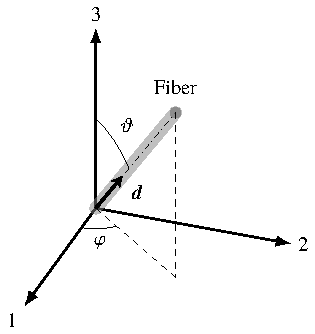
\includegraphics[scale=0.8]{direction_vector}
	\caption{Representation of direction vectors in $\mathbb{S}^2$}
	\label{fig:direction_vector}
\end{figure}%



	
	Generally, the continuous orientation PDF can be approximated in the case of $N$ discrete non-zero values of the oriented function $f(\tena{d})$ by an empirical distribution density in the form~\autocite{Kanatani.1984}
	\begin{equation}
		\psi(\tena{d})=\frac{1}{N}\sum_{j=1}^N\delta(\tena{d}-\tena{d}^{(j)}),
	\end{equation}
	where by means of the Dirac delta generalised function ($\delta$), the existence of a fibre along a particular direction in $\mathbb{S}^2$ is captured:
	\begin{equation}
		\delta(\tena{d}-\tena{d}^{(j)})= \frac{1}{\sin\vartheta^{(j)}} \delta(\varphi-\varphi^{(j)})\delta(\vartheta-\vartheta^{(j)}).
	\end{equation}
	Thus, the average value obtained from a continuous oriented function in Eq.~\eqref{eq:odist} can be replaced by $N$ contributions from a discretised counterpart:
	\begin{equation}
		\averot{f} =\frac{1}{N}\sum_{j=1}^N f(\tena{d}^{(j)}),
	\end{equation}
	which is equivalent to Kanatani's orientation tensor of first kind~\autocite{Kanatani.1984}. Alternative versions are available in literature; for instance in the context of fibre-reinforced composites, a weighted average is used such that the volume of fibres ($V_\text{f}$) is the scaling parameter~\autocite{Muller.2016}:
	\begin{equation}\label{eq:OTw}
		\averot{f}^\prime =\frac{1}{V}\sum_{j=1}^{N} V^j_\text{f}\; f(\tena{d}^{(j)}),
	\end{equation}
	where $V$ is the total volume of fibres in the sample.
%	This formula can be applied to layers 
%	\begin{equation}
%		\averot{f}_\text{layer} =\frac{1}{V_\text{layer}}\sum_{j=1}^{N_\text{layer}} V_\text{f}\; f(\tena{d}^{(j)}),
%	\end{equation}	
%	where $V_\text{layer}$ is the volume of the layer and $N_\text{layer}$ is the number of fibres per layer. Herein, per-element normalisation is applied:
%	\begin{equation}
%		\averot{f}_\text{element} =\frac{1}{V_\text{element}}\sum_{j=1}^{N_\text{fiber/element}} V_\text{f}\; f(\tena{d}^{(j)}),
%	\end{equation}
%	where $V_\text{element}$ is the volume of the element and $N_\text{fiber/element}$ is the number of fibres in that element.
\subsection{Averaged Orientation Tensor}
	Defining the \textit{orientation tensor} as
	\begin{equation}
		\tenb{A}\equidef \tena{d}\dyad\tena{d},\label{eq:ot}
	\end{equation}
	results in an \textit{averaged orientation tensor} of order $2k$\footnote{mathematically, it is shown by $\tenn{H}{2k}\equiv\averot{\tena{d}^\tenpow{2k}}$ , and thus it is a tensor of order $2k$.} or orientation tensor of first kind (moment tensor)~\autocite{Kanatani.1984}:
	\begin{equation}
		\ten{H}_k\equidef \averot{\tenb{A}^\tenpow{k}}.\label{eq:ot1}
	\end{equation}
	Since $\tenb{A}$ has no odd powers, it is symmetric, and thus its average $\ten{H}_k$ is also symmetric~\autocite{Kanatani.1984,Comon.2008}. Note that this formulation automatically rules out the trivial odd-ordered combinations of orientation vectors. Moreover, lower order averaged orientation tensors are obtained by contracting higher ones: 
	\begin{equation}
	\ten{H}_{k-1} = \ten{H}_{k}\dscp\unitb,\qquad\qquad \forall k\in\Natural\ge2,
	\end{equation}
	and therefore they are not independent~\autocite{Advani.1987}. This is another incentive to use the orientation tensor of the third kind of various orders since they are independent from each other~\autocite{Kanatani.1984}. Both types are similar, and thus share the same eigenvalues and eigenvectors. Therefore, either one can be used in spectral analysis.
	
	The second-order orientation tensor $\tenb{H}_{1}=\averot{\tenb{A}}$ is frequently used in the literature; for simplicity, it will be denoted by $\tenb{H}$ henceforth. The fourth-order orientation tensor $\tend{H}_{2}=\averot{\tenb{A}\dyad\tenb{A}}$ (denoted by $\tend{H}$) is also available in the literature, see~\autocite{Vasta.2014}. In either case, symmetry reduces the number of independent parameters. For instance in~\autocite{Gasser.2006}, a `generalised structure tensor' is introduced to capture the orientation of collagen fibres in soft tissue (equivalent to the second-order averaged orientation tensor). As mentioned earlier, the orientation PDF is centro-symmetric, and thus $\psi(-\tena{d})=\psi(\tena{d})$. An additional symmetry axis $\tena{d}_0$ could also exist if $\psi(\tenb{Q}\scp\tena{d}_0)=\psi(\tena{d}_0)$, where $\tenb{Q}$ belongs to the symmetry group of all proper orthogonal tensors about $\tena{d}_0$. If it is assumed that the polar axis coincides with $\tena{d}_0$, the averaged orientation tensor can be represented by a single dispersion parameter. In the absence of such symmetry in an $n$-dimensional space, evaluation of the $2k$-order average orientation tensor requires the calculation of $n^{2k}$ integrals over $\mathbb{S}^2$ (without considering its universal symmetry). A $k$-th order averaged orientation tensor can be represented by $k$ scalars provided that a transversely isotropic orientation PDF exists~\autocite{Hashlamoun.2017}.
	 
	%$k_1$:
%	\begin{equation}
%		\tenb{H}=k_1\unitb +(1-3k_1)\tenb{A}_0,
%	\end{equation}
%	where $\tenb{A}_0\equidef\tena{d}_0\dyad \tena{d}_0$ is the orientation tensor with the additional symmetry axis. Consequently, the orientation PDF becomes independent of the polar angle, i.e., $\psi(\vartheta,\varphi)\equiv\psi(\varphi)$. It is shown that the value of the dispersion parameter is readily calculated from
%		\begin{equation}
%			k_1=\pi\int_{0}^{\pi}\psi(\varphi)\sin^3\varphi\;\dif\varphi.
%		\end{equation}
 	Transverse isotropy of the orientation PDF does not exist in most practical cases, at least not globally. For instance in a short FRC, no symmetry groups might be found for the whole specimen or at the other extreme, even a complete isotropy might be detected for completely random samples; either case might be unsophisticated characterisations of meso-structure. On the other hand, a symmetry axis might just exist locally where only a few fibres (ideally one) exist(s) whereas demanding such a condition for the whole sample is a very strong one. The remedy might be an auxiliary map with enough resolution so that our assumption of transverse isotropy carries small errors. In the current study, the resolution of the auxiliary maps is set according to the finite elements of composite. Obviously, other finer/coarser arrangements are possible. 

%	\paragraph{Additive decomposition of orientation tensor} In~\autocite{Shertzer.2011}, the second-order average orientation tensor is additively decomposed to its dilatoric (isotropic or volumetric) and deviatoric (or isochoric) components: 
%	\begin{equation}
%	\tenb{H}_1=\tenb{H}^\vol_1+\tenb{H}^\dev_1.
%	\end{equation}
%	The deviatoric component is identical to Kantani's orientation tensor of third kind. The isotropic component represents the part of averaged orientation tensor that cannot identify any preferred orientation. Thus, meso-structure is deemed isotropic provided that the deviatoric component vanishes. This state is equivalent to having recurring eigenvalues for the orientation tensor. This paragraph is not correct since the orientation tensor of third kind is a traceless symmetrical tensor and the aforementioned additive decomposition does not product such as result. An decomposition into irreducible tensors is required that gives a second-order tensor as the sum of zeroth-, first-, and second-order tensors.
\subsection{Homogenisation}
	\paragraph{Enhanced rule of mixture} Consider a transversely isotropic material with the axis of symmetry along the 1-direction and the 2-3 isotropy plane. From the strength-of-material point of view, homogenisation formulas for unidirectional composites, i.e., the rule of mixture (RoM) and the inverse rule of mixture (IRoM), are based on the iso-strain and iso-stress assumptions, respectively:
	\begin{subequations}
	\begin{alignat}{2}\label{eq:rom}
		E_1 		=\;& \zeta_\text{f}E_\text{f}          &&+\zeta_\text{m}E_\text{m},\\
		\frac{1}{E_2}	=\;& \frac{\zeta_\text{f}}{E_\text{f}} &&+ \frac{\zeta_\text{m}}{E_\text{m}},
	\end{alignat}
	\end{subequations}
	where $\zeta$ is the volume fraction and $E$ shows the elastic modulus. Subscripts of `$\text{f}$' and `$\text{m}$' are used to denote fibre and matrix phases, respectively. The elastic moduli $E_1$ and $E_2$ set the upper and lower bounds of stiffness and are in accordance with the longitudinal and transverse stiffnesses, respectively. An efficiency parameter $\varkappa$ is used to further adjust these bounds by altering the contribution of fibres. The result is the enhanced rule of mixture (En-RoM)~\autocite{Summerscales.2019} 
	\begin{subequations}
	\begin{alignat}{2}
		\hat{E}_1 &= \varkappa\zeta_\text{f}E_\text{f}+\zeta_\text{m}E_\text{m},\label{eq:enrom}\\
		\frac{1}{\hat{E}_2} &=\frac{\zeta_\text{f}}{\varkappa_\text{a} E_\text{f}}+ \frac{\zeta_\text{m}}{E_\text{m}},\label{eq:enirom}
	\end{alignat}
	\end{subequations}
	with $\varkappa \equidef \varkappa_\text{a}\varkappa_\text{d}\varkappa_\text{l}\varkappa_\text{o}$ where $\varkappa_\text{a}$ is the fibre area correction factor (FACF), $\varkappa_\text{d}$ is the fibre diameter distribution factor (FDDF), $\varkappa_\text{l}$ is the fibre length distribution factor (FLDF), and $\varkappa_\text{o}$ is the fibre orientation distribution factor (FODF), respectively. Well-characterised fibre diameters assign a unit value to FDDF; a unit value is also assigned to FLDF since continuous fibres are the focus of the current study. The FODF can be estimated by Krenchel's formula~\autocite{Krenchel.1964}
		\begin{equation}
			\varkappa_\text{o}=\sum_n a_n\cos^4\theta,\label{eq:Krenchel}
		\end{equation}
	where $a_n$ is the fraction of fibres making a $\theta$ angle with the applied load. The FACF is suggested by~\autocite{Virk.2009} and is used to rectify the underestimation of stiffness and strength due to an overestimation in measuring the cross-section area (CSA) of fibres. For jute fibres, a typical value of 1.42 was suggested in the same study. 
	
	In the same spirit, the relation for shear modulus ($\hat{G}_{12}$) is established
	\begin{subequations}
	\begin{alignat}{2}
		\frac{1}{\hat{G}_{12} } &=\frac{\zeta_\text{f}}{\varkappa_\text{a} G_\text{f}}+ \frac{\zeta_\text{m}}{G_\text{m}},\label{eq:enirom2}
	\end{alignat}
	\end{subequations}
	The Poisson's ratio in anisotropic elasticity could be defined as $\nu_{ij}\equidef -\sfrac{\varepsilon_j}{\varepsilon_i}$ and for an orthotropic material, due to the symmetry of the compliance matrix, the relation $ \sfrac{\nu_{ij}}{E_i}  =\sfrac{\nu_{ji}}{E_j}$ is established. The Poisson's ratio of the composite $\nu_{12}$ is obtained from
	\begin{equation}
		\nu_{12}= \zeta_\text{f}\nu_\text{f}+\zeta_\text{m}\nu_\text{m}.\label{eq:enrom2}\\
	\end{equation}
	Finally, the transversely isotropic elastic compliance matrix $\tend{C}^\inv$ for the composite along the $1$-axis, i.e., when 2-3 is the plane of symmetry, is established using contracted Voigt notation:
	\begin{equation}\label{eq:Cinv}
	\mat{C}^\inv=
	\left[
	\begin{array}{cccccc}
		\frac{1}{\hat{E}_1} & -\frac{\nu_{21}}{\hat{E}_2} & -\frac{\nu_{21}}{\hat{E}_2} &            0            &            0            &            0            \\
		                      &       \frac{1}{\hat{E}_2}        & -\frac{\nu_{23}}{\hat{E}_2} &            0            &            0            &            0            \\
		                      &                                   &       \frac{1}{\hat{E}_2}        &            0            &            0            &            0            \\
		                      &                                   &                                   & \frac{1}{\hat{G}_{23}} &            0            &            0            \\
		                      &            \text{sym}             &                                   &                         & \frac{1}{\hat{G}_{12}} &            0            \\
		                      &                                   &                                   &                         &                         & \frac{1}{\hat{G}_{12}}
	\end{array}
	\right],
	\end{equation}		
	where $\hat{G}_{23}=\frac{\hat{E}_2}{2(1+\nu_{23})}$. 
%	The Kelly-Tyson model~\autocite{Kelly.1965} is used to evaluate the strength of unidirectional composites $\sigma^\prime_\text{c}$. Following the approach in extending Eq.~\eqref{eq:rom} to Eq.~\eqref{eq:enrom}, the enhanced Kelly-Tyson model (En-KT) is introduced for natural fibres:
%	\begin{equation}
%		\sigma^\prime_\text{En,c} = \kappa \zeta_\text{f}\sigma^\prime_\text{f}+\zeta_\text{m}\sigma^*_\text{m},\label{eq:en-KT}
%	\end{equation}
%	where $\sigma^\prime_\text{f}$ is the strength of fibre, and $\sigma^*_\text{m}$ is the stress in the matrix at composite failure---assuming a dominant fibre failure mechanism, i.e., the matrix is more compliant compared to the fibre under iso-strain conditions. This estimate is used to check the failure of the homogenised elements. 
	
	Equations~\eqref{eq:enrom} to \eqref{eq:enrom2} are generally used globally and in order to apply them locally, the efficiency parameter and the volume fraction must be localised. The volume fraction is readily calculated from its auxiliary map and all of the parameters involved in calculation of efficiency parameter $\varkappa$ can be assumed constant except for the FODF since its spatial variation is not negligible---specially in the cases where fibre clustering or resin-rich volumes exist. Thus, the second auxiliary map would be that of the orientation tensor. 
		
	Using the obtained material properties, the elastic tensor for a transversely isotropic material is in hand. The axis of symmetry is obtained from the spectral analysis of the orientation tensor, i.e., the principal direction of the material is denoted by the eigenvector of the maximum eigenvalue of the orientation tensor. This tensor is used to calibrate the more general formulation discussed in the following section.
	
	
%	An alternative to the global formulation is using Krenchel's formula in Eq.~\eqref{eq:Krenchel} 
%			 the FODF is calculated in two ways: either replaced by the local orientation tensor, or calculated using the global overall orientation of the spectral analysis.
%		
	
	
	

%	The use of 2D embedded fibre elements artificially increases the volume of the matrix since in the fibre-occupied volume, matrix still exists. Thus, this should be considered in the calculations. This can be done either by modifying the elastic moduli or applying a correction factor to the volume of the matrix, e.g., by reducing the overall thickness of the composite.

\subsection{Constitutive Material Model}	
	In~\autocite{Spencer.1984}, the formulation of elastic moduli of composites was carried out by setting up a quadratic free energy function in which the invariants of the orientation tensor $\tenb{H}$ and infinitesimal strains tensor $\tenb{\epsilon}$ were incorporated. The result is rearranged in the following (minor and major) symmetric form for the averaged elastic tensor:
	\begin{equation}\label{eq:C}
	\averot{\tend{C}} = 3\lambda\unitd^\vol+2G_\text{T}\unitd^\sym +2\alpha (\tenb{H}\dyad\unitb)^\sym+4(G_\text{L}-G_\text{T})(\tenb{H}\dyadd\unitb)^\sym +\beta\tend{H},
	\end{equation}
	where out of the five constants, $\lambda$, $\alpha$, and $\beta$ are functions of elastic properties of an aligned FRC and $G_\text{L}$ and $G_\text{T}$ are its shear moduli in the longitudinal and transverse directions. All these parameters are calculated based on the relations of the previous section. The orientation tensor adjusts the deviation from this perfectly aligned status. Overall, the symmetry group of this constitutive tensor is all the orthogonal transformations about the axis of symmetry. This form is identical to what is proposed in~\autocite{Advani.1987} or more generally in~\autocite{Cowin.1985}. Herein, the rearranged representation concisely illustrates the individual symmetrical terms in direct notation. Furthermore, the 4th-order averaged orientation tensor $\tend{H}$ can be replaced by means of various closure approximations; see~\autocite{Breuer.2019,Advani.1990}.% the last term is replaced by a quadratic approximation, . Herein, a quadratic approximation is used; see~\autocite{Breuer.2019}.

	Considering the fact that the invariant $\tr(\tenb{H})$ is unit, the model in Eq.~\eqref{eq:C} is calibrated for the principal material directions. This is the case where symmetry reduces the the number of independent parameters to one. Namely, the only non-zero component of $\tenb{H}$ becomes its maximum eigenvalue. Thereby, the constitutive equation of transversely isotropic material becomes available for any arbitrary orientation tensor. Accordingly, the material parameters of Eq.~\eqref{eq:C} can be readily related to the Voigt components of the elastic tensor in the principal direction---which is obtained by inverting Eq.~\eqref{eq:Cinv}:
	\begin{subequations}
%	\begin{alignat}{2}
%		B_1\equiv&\;\beta  			&&= C_{11}+C_{22}-2C_{12}-4C_{66},\\
%		B_2\equiv&\;\alpha &&=C_{12}-C_{23},\\
%		B_3\equiv&\;\mu_\text{LL}-\mu_\text{TL}&&=C_{66}+0.5(C_{23}-C_{22}),\\
%		B_4\equiv&\;\lambda&&=C_{23},\\
%		B_5\equiv&\;\mu_\text{TL}&&=0.5(C_{22}-C_{23}).
%	\end{alignat}
	\begin{alignat}{2}
		\beta  	&= C_{11}+C_{22}-2C_{12}-4C_{66},\\
		\alpha  &=C_{12}-C_{23},\\
		G_\text{L}-G_\text{T}&=C_{66}+\half(C_{23}-C_{22}),\\
		\lambda&=C_{23},\\
		G_\text{T}&=\half(C_{22}-C_{23}),
	\end{alignat}
	\end{subequations}	
	where $G_\text{T}\equiv \hat{G}_{23}$ and $G_\text{L}\equiv \hat{G}_{12}$ retain their physical meanings.

	After incorporating the averaged orientation tensor, an explicit formulation of the final elasticity tensor for any arbitrary orientation can be obtained from Eq.~\eqref{eq:C}. By assuming $\nu_\text{23}= 0$ and a planar distribution of fibres on the 1-2 plane, the non-zero components of the elastic tensor become
	\begin{subequations}
	\begin{alignat}{2}
		C_{11}=\;&\lambda + 2G_\text{T} + 4(\half\alpha+G_\text{L}-G_\text{T})H_{11}+\beta H_{11}^2,\\
		C_{12}=\;&\lambda +\alpha(H_{11}+H_{22})+\beta H_{11}H_{22},\\
		C_{13}=\;&\alpha H_{11}+\lambda,\\
		C_{16}=\;&\alpha H_{11} + (\alpha+2G_\text{L}-2G_\text{T})H_{12}+\beta H_{11}H_{12},\\
		C_{22}=\;&\lambda + 2G_\text{T} + 4(\half\alpha+G_\text{L}-G_\text{T})H_{22}+\beta H_{22}^2,\\
		C_{23}=\;&\alpha H_{22}+\lambda,\\
		C_{26}=\;&\alpha H_{22} + (\alpha+2G_\text{L}-2G_\text{T})H_{12}+\beta H_{22}H_{12},\\
		C_{33}=\;& \lambda + 2G_\text{T},\\
		C_{36}=\;& \alpha H_{12},\\
		C_{44}=\;& (G_\text{L}-G_\text{T})H_{22}+G_\text{T},\\
		C_{45}=\;& (G_\text{L}-G_\text{T})H_{12},\\
		C_{55}=\;& \beta H_{12}^2 (G_\text{L}-G_\text{T})(H_{11}+H_{22})+G_\text{T},\\
		C_{66}=\;&G_\text{T} + (G_\text{L}-G_\text{T})(H_{11}+H_{22})+\beta H_{12}^2.
	\end{alignat}
	\end{subequations}
	The plane stress case governs the behaviour of thin laminates and is of interest in the current study. Therefore, the reduced stiffness elastic tensor ($\tilde{\mat{C}}$)~\autocite{Herakovich.1998,Altenbach.2010c} can be calculated from the evaluated components:	
	\begin{equation}\label{eq:plane}
	\tilde{\mat{C}}_{\text{2D}}=
	\left[
		\begin{array}{ccc} 
			\tilde{C}_{11}  & \tilde{C}_{12} & \tilde{C}_{16}\\
					& \tilde{C}_{22} & \tilde{C}_{26}\\
			\text{sym}		&		 & \tilde{C}_{66}\\
		\end{array}	
	\right],
	\end{equation}
	with 
	\begin{equation}
	\tilde{C}_{ij}\equidef C_{ij}-\frac{C_{i3}C_{3j}}{C_{33}},\qquad\qquad\forall i,j\in\{1,2,6\}.
	\end{equation}

\begin{comment}

\subsection{Generalised Rule of Mixture}
	In order to generalise the enhanced rule of mixture (En-RoM)~\autocite{Summerscales.2019}, the fibre efficiency parameter ($F$) is introduced:
	\begin{equation}
		f \equidef \kappa\eta_\text{d}\eta_\text{l}\eta_\text{o},
	\end{equation}
	where $\kappa$ is the fibre area correction factor (FACF), $\eta_\text{d}$ is the fibre diameter distribution factor (FDDF), $\eta_\text{l}$ is the fibre length distribution factor (FLDF), and $\eta_\text{o}$ is the fibre orientation distribution factor (FODF), respectively. Herein, FODF is dropped since orientation tensors are used in a local sense. Also well-characterised fibre diameters assign a unit value to FDDF; a unit value is also assigned to FLDF, and thus the effective elastic tensor of fibres is readily amended:
	\begin{equation}
		\tend{C}^{\text{(f)}} \equidef \kappa\hat{\tend{C}}^\text{(f)}.
	\end{equation} 
	% TODO check the first citation and find the second citation
	%	TECHNICAL MISTAKE.		folllowing paragraph is removed.
	%	Furthermore, in the case of using embedded fibres, parametric studies show that the nominal and true volume fractions result in different responses especially in higher volume fractions~\autocite{Javanbakht.2016b}. Thus, this discrepancy is compensated by modifying either the thickness of the model composite or its material properties~\autocite{}. In the sprite of En-RoM, the model correction factor $m$ is applied:
	%	\begin{equation}
	%		\tend{C}^{\text{(m)}} \equidef m\,\hat{\tend{C}}^\text{(m)},
	%	\end{equation}		
	%	which can be interpreted as reducing the efficiency of the matrix ($\eta_\text{m}<1$).
	
	In mean-field methods, the volume averaging of an arbitrary field ($\tend{T}$) over the $\Omega$ domain is defined as
	\begin{equation}
	\avevol{\tend{T}} \equidef \int_{\Omega}\tend{T}(\tena{x})\dif\Omega,
	\end{equation}
	where $\tena{x}$ is the position vector. In a biphasic material, the domain consists of fibre (f) and matrix (m) volumes, i.e., $\Omega_\text{f} \cup \Omega_\text{m}=\Omega$ and $\Omega_\text{f} \cap \Omega_\text{m}=\varnothing$. To set up the micro-mechanical formulation for a multi-phase continuum, the micro-constitutive relation between the stress and strain of the $p$ phase is
	\begin{alignat}{2}
	\tenb{\sigma}^\text{(p)} &= \tend{C}^\text{(p)}\dscp\tenb{\epsilon}^\text{(p)},\qquad\qquad\forall\text{p}\in\{\text{f},\text{m}\},
	\end{alignat}
	where $ \tend{C}^\text{(p)}$ is the elastic stiffness of the phase $\text{p}$. The averaged macro-constitutive relation for the homogenised medium is
	\begin{alignat}{2}
		\avevol{\tenb{\sigma}} &= \tend{C}\dscp\avevol{\tenb{\epsilon}},
	\end{alignat}
	where $\tend{C}$ is the effective elastic stiffness of the multi-phase medium. The average stress and average strain of the medium are $\avevol{\tenb{\epsilon}}=\sum\zeta^{(p)}\tenb{\epsilon}^{(p)}$ and $\avevol{\tenb{\sigma}}	=\sum\zeta^{(p)}\tenb{\sigma}^{(p)}$ where $\zeta^{(p)}=\sfrac{\Omega_\text{p}}{\Omega}$ is the volume fraction of the $p$ phase. In the next step, localisation tensors~\autocite{Hill.1963} are used to relate the overall averaged properties to the phase-averaged ones:
	\begin{alignat}{2}
	\forall\text{p}\in\{\text{f},\text{m}\}:\left\{
	\begin{array}{rl}
		\avevol{\tenb{\epsilon}}^\text{(p)} &= \tend{A}^\text{(p)}\dscp\avevol{\tenb{\epsilon}},\\[0.2cm]
		\avevol{\tenb{\sigma}}^\text{(p)} 	&= \tend{A}^\text{(p)}\dscp\avevol{\tenb{\sigma}}.
	\end{array}\right.,
	\end{alignat}
	and obtain the effective elastic tensor
	\begin{equation}
	\tend{C}=\sum_\text{(p)}\zeta^\text{(p)} \tend{A}^\text{(p)}\dscp\tend{C}^\text{(p)}.
	\end{equation}
	Adopting Voigt's assumption demands $ \avevol{\tenb{\epsilon}^\text{(f)}}\equimust\avevol{\tenb{\epsilon}^\text{(m)}}\equimust\avevol{\tenb{\epsilon}}$ that results in $\sum_\text{(p)}\zeta^{(p)}\tend{A}^\text{(p)}=\unitd^\sym$. Finally, the general form of rule of mixture for a bi-phasic medium is obtained
	\begin{equation}
	\tend{C}=\sum_\text{(p)}\zeta^\text{(p)}\tend{C}^\text{(p)}.
	\end{equation}


	
	%TODO non-local formulation
	%	Setting up a local model might result in very localised behaviour when softening behaviour is involved. One remedy is to use a non-local scheme by replacing the local strain field by its weighted average, which requires introducing a length parameter ($\ell$). So in the current model, the orientation is localised while the non-local strain field is used.

\subsection{Spectral Decomposition}
	In the principal coordinates and in the most general case, the second order orientation tensor reduces to three distinct eigenvalues: $\lambda_\text{max}$, $\lambda_\text{int}$, and $\lambda_\text{min}$. Due to the negligible out-of-plane orientation of fibres, especially for laminar meso-structures, the minimum eigenvalue vanishes, i.e., $\lambda_\text{min}=0$. Moreover, since $\tr{\tenb{H}}=1$, the the second-order average orientation tensor decomposes to:
	\begin{equation}
		\tenb{H}=\lambda_\text{max}\base^\prime_1\dyad\base^\prime_1+(1-\lambda_\text{max})\base^\prime_2\dyad\base^\prime_2,
	\end{equation}
	where $\base^\prime_1$ is assumed to be the averaged preferred direction of the fibres. 
	
	Rotation about an arbitrary fixed axis, denoted by the direction vector $\tena{m}$, is carried out by the proper unimodular rotation tensor~\autocite{Eremeyev.2013}:
	\begin{equation}
		\tenb{R}_{\scriptsize\tena{m}}(\alpha)=\tena{m}^\tenpow{2}+\cos\alpha(\unitb-\tena{m}^\tenpow{2})-\sin\alpha\;\tena{m}\cross\unitb,
	\end{equation}
	where $\alpha$ is the rotation angle about the axis. Note that the first term is the projection tensor along the axis $\tena{m}$, the second term is the projection tensor over the corresponding plane of the axis, and the third term represents a skew-symmetric second-order tensor.
	
	Assume an arbitrary direction denoted by direction vector $\tena{a}_0$ that makes an angle $\alpha_0=\cos^{-1}(\tena{a}_0\scp\base^\prime_1)$ with the maximum principal direction of $\tenb{H}$. Rotation of $\tenb{H}$ from principal direction is carried out by $\tenb{R}_{\scriptsize\tena{m}_0}(\alpha_0)\Rayleigh\tenb{H}$ where $\tena{m}_0=\frac{\tena{a}_0\cross\base^\prime_1}{\norm{\tena{a}_0\cross\base^\prime_1}}$ is the axis of rotation.

\subsection{Direction-dependent Elastic and Bulk Moduli}
	The direction-dependent elastic modulus 
	\begin{equation}
		E(\tena{d})=(\tena{d}^\tenpow{2}\dscp\tend{C}^\inv\dscp\tena{d}^\tenpow{2})^\inv,
	\end{equation}
	and the direction-dependent bulk modulus
	\begin{equation}
		K(\tena{d})=\frac{1}{3}(\unitb\dscp\tend{C}^\inv\dscp\tena{d}^\tenpow{2})^\inv,
	\end{equation}
	are evaluated with respect to the fixed arbitrary direction $\tena{d}$ where $\tend{C}^\inv$ is the elastic compliance tensor.



% --------------------------------------------------------------------------------------------------
\subsection{Representing the Elastic Stiffness of the Composite}
	The response of the composite is equivalent to the contributions from the isotropic matrix, isotropic fibres, and anisotropic fibres (considered by means of the orientation tensor).



	
\subsection{Formulation In Terms of Projectors}
	In a transversely isotropic materials the normal of the isotropic transverse plane denotes the axis of symmetry (along the axial direction). The introduced orientation tensor ($\tenb{A}$) can be regarded as a projector along the axial direction. By adding the projector of the transverse plane ($\tenb{T}$), a complete projector set is obtained:
	\begin{alignat}{2}
		\tenb{A}\equidef\; &\tena{d}\dyad\tena{d},\tag{\ref{eq:ot} revisited}\\
		\tenb{T}\equidef\; &\unitb - \tenb{a}
	\end{alignat}
	where the bi-orthogonality ($\tenb{A}\scp\tenb{T}=\tenb{T}\scp\tenb{A}=\nullb$) and idempotency ($\tenb{A}^n=\tenb{A}$ and $\tenb{T}^n=\tenb{T}$) of the projectors are satisfied.
	
\subsection{Plane Strain Formulation}	
	In this section, the general formula is reduced to the simple plane strain case. The orientation PDF becomes independent of the polar angle, i.e., $\psi(\vartheta,\varphi)\equiv\psi(\varphi)$.




\subsection{Matrix Representation of a General 4th-order Tensor}
	Often in order to carry out numerical analysis, the matrix presentation of tensors is required. For instance, general second- and fourth-order tensors can be arranged in terms of $3\times 3$ matrices (or $9\times 1$ column vectors) and $9\times 9$ matrices (or $81\times 1$ column vectors), respectively. Similarly, all tensorial operations should be translated to the algebra of matrices.


\subsection{Matrix Representation of Elastic Tensor}
	Fedorov's~\autocite{Fedorov.1968} representation of the elastic tensor $\tend{C}$ is obtained by using the orthonormal basis
	\begin{subequations}
	\begin{alignat}{2}
		\tena{e}^\prime_1\equidef&\;&         \base_1\dyad&\base_1,\\
		\tena{e}^\prime_2\equidef&\;&         \base_2\dyad&\base_2,\\
		\tena{e}^\prime_3\equidef&\;&         \base_3\dyad&\base_3,\\
		\tena{e}^\prime_4\equidef&\;&\sqrt{2}(\base_2\dyad&\base_3)^\sym,\\
		\tena{e}^\prime_5\equidef&\;&\sqrt{2}(\base_1\dyad&\base_1)^\sym,\\
		\tena{e}^\prime_6\equidef&\;&\sqrt{2}(\base_1\dyad&\base_1)^\sym,
	\end{alignat}
	\end{subequations}
	to obtain an equivalent six-by-six elasticity matrix $\mat{C}$:
	\begin{equation}\label{eq:fedorov}
		\mat{C}_{ij} \equidef 	\tena{e}^\prime_i\scp\tend{C}\scp\tena{e}^\prime_j\qquad\qquad\forall i,j\in\{1,2,...,6\}.
	\end{equation}
	This matrix representation results in the following form of generalised Hooke's law:
	
	Note that Eq.~\eqref{eq:fedorov} is bridging between the tensorial and matrix notations. The introduced basis vectors are to ensure the equivalence between the following tensorial and matrix operations~\autocite{Nordmann.2018}:
	
	
	For the case of transversely isotropic material (hexagonal crystals), 5 material parameters plus the axis of symmetry must be known~\autocite{Bohlke}.
	
\subsection{Anisotropy measures}
	
	 
\subsection{Creating an observation mesh}
	If a $m\times n$ uniform mesh is used for the FE analysis, the same mesh could be used to monitor the orientation of elements. 
	


\pagebreak
% --------------------------------------------------------------------------------------------------
\subsection{Anisotropic Failure Criterion}
	A general failure criterion for anisotropic materials can take the following form~\autocite{Goldenbart}:
	\begin{equation}%TODO by adding a contraction operator and a sigma this can be more compact
		f\equidef \sum_{k=1}^{n}
		(\tenb{\sigma}^\tenpow{k}\contract\tenn{S}{2k})^{\alpha_k} \le 1,\qquad\qquad \alpha_k \in \Real,		
%		(\tenb{\sigma}\dscp\tenb{S})^\alpha + (\tenb{\sigma}^\tenpow{1}\contract\tend{S})^\beta +
%		(\tenb{\sigma}^\tenpow{2}\contract\tenn{S}{6})^\gamma + \ldots\le 1,\qquad\qquad \alpha, \beta, \gamma, ... \in \Real,
	\end{equation}
	where Cauchy stress tensor ($\tenb{\sigma}$), and strength tensors ($\ten{S}$) are related via the scalars ($\alpha_k$). By choosing the appropriate scalars and the order of tensors, other similar failure criteria are obtained. For instance, Tsai-Wu criterion~\autocite{Tsai.1971} is a special case for which the linear and quadratic terms are used~($\alpha_1=\alpha_2=1$), i.e., the linear combination of first and second order tensors:
	\begin{equation}
		f_\text{Tsi-Wu}\equidef \tenb{\sigma}\dscp\tenb{S} + (\tenb{\sigma}\dyad\tenb{\sigma})\contract\tenn{S}{4} =\tenb{\sigma}\dscp\tenb{S} + \tenb{\sigma}\dscp\tend{S}\dscp\tenb{\sigma}^\tran.
	\end{equation}	 

	
	A scalar-valued function of Cauchy stress tensor ($\tenb{\sigma}$), orientation tensor ($\tenb{H}$) and fibre volume fraction ($v_\text{f}$) is assumed~\autocite{Cowin.1986}:
	\begin{equation}
		f\equiv f(\tenb{\sigma}, \tenb{H}, v_\text{f}).
	\end{equation}
	Since the anisotropy of the continuum is incorporated by means of the orientation tensor, $f$ must succumb to every symmetry, i.e., it must satisfy the isotropy condition:
	\begin{equation}
		f(\tenb{\sigma}, \tenb{H}, v_\text{f})\equimust f(\tenb{Q}\Rayleigh\tenb{\sigma}, \tenb{Q}\Rayleigh\tenb{H}, v_\text{f}),
	\end{equation}
	where $\tenb{Q}$ is the orthogonal rotation tensor. Alternative to satisfying this equation, a form-invariant anstaz could be considered by including all the invariants of the parameters in the function~\autocite{Boehler.1987}:
	\begin{equation}
		f\equiv f\big(
		\tr{\tenb{\sigma}},\tr{\tenb{\sigma}^2},\tr{\tenb{\sigma}^3},
		\tr{\tenb{H}},\tr{\tenb{H}^2},\tr{\tenb{H}^3},
		\tr{(\tenb{\sigma}\scp\tenb{H})},\tr{(\tenb{\sigma}\scp\tenb{H}^2)},\tr{(\tenb{\sigma}^2\scp\tenb{H})},\tr{(\tenb{\sigma}^2\scp\tenb{H}^2)},v_\text{f}\big).
	\end{equation}
	where $\tr{(\square)}\equidef\tenb{I}\dscp\square$ indicates the trace operator.	
	\begin{equation}
		\tenb{S} =\;g_1\unitb+g_2\tenb{H}+g_3\tenb{H}\scp\tenb{H}
	\end{equation}	
	\begin{alignat}{5}
		\tend{S} =\;&&	f_1 \unitd^\vol 
					&+&f_2 (\tenb{H}\dyad\unitb)^\sym 
					&+&f_3 (\tenb{H}\scp\tenb{H}\dyad\unitb)^\sym\\\nonumber
					&+&f_4 (\tenb{H}\dyad\tenb{H})
				    &+&f_5 (\tenb{H}\scp\tenb{H}\dyad\tenb{H})^\sym 
					&+&f_6 (\tenb{H}\scp\tenb{H}\dyad\tenb{H}\scp\tenb{H})^\sym \\\nonumber
					&+&f_7 \unitd^\sym
					&+&f_8 \big[(\tenb{H}\dyadu\unitb)^\sym + (\unitb\dyadu\tenb{H})^\sym\big]
					&+&f_9 \big[(\tenb{H}\scp\tenb{H}\dyadu\unitb)^\sym + (\unitb\dyadu\tenb{H}\scp\tenb{H})^\sym\big].
	\end{alignat}
% not sure about these parameters. If they are the same parameters as those of the elastic stiffness tensor, the following equations are correct.
%	where
%	\begin{alignat}{5}
%		f_i\equiv f_i(\tr{\tenb{H}},\tr{\tenb{H}^2},\tr{\tenb{H}^3},v_\text{f})\qquad\qquad\forall i\in\{1,...,9\}.
%	\end{alignat}		


\subsection{Anisotropic Failure Criterion}


	Shear strength of composite is assumed to be near

	A general failure criterion for anisotropic materials can take the following form~\autocite{Goldenblat.1966}:
	\begin{equation}
		% Original expanded form:
		%(\tenb{\sigma}\dscp\tenb{S})^\alpha + (\tenb{\sigma}^\tenpow{1}\contract\tend{S})^\beta +(\tenb{\sigma}^\tenpow{2}\contract\tenn{S}{6})^\gamma + \ldots\le 1,\qquad\qquad \alpha, \beta, \gamma, ... \in \Real,
		% is expressed in a more compact way:
		f\equidef \sum_{k=1}^{n}
		(\tenb{\sigma}^\tenpow{k}\contract\tenn{S}{2k})^{\alpha_k} \le 1,\qquad\qquad \alpha_k \in \Real,
	\end{equation}
	where Cauchy stress tensor ($\tenb{\sigma}$), and strength tensors ($\ten{S}$) are related via the scalars ($\alpha_k$). Full contraction ($2k$-times here) is denoted by the $\contract$ symbol. The advantage of this mathematical form is that odd and even terms naturally appear, and thus the strength in compression and tension can be distinguished. This facility is not available in criteria with only quadratic terms, e.g., Tsai-Hill. Therefore, this form could be regarded as a more general criterion with which other more restricted failure criteria are obtained by choosing the appropriate scalars and order of tensors. For instance, Tsai-Wu criterion~\autocite{Tsai.1971} is a special case for which the linear and quadratic terms are used~($\alpha_1=\alpha_2=1$), i.e., the linear combination of first and second order tensors:
	\begin{equation}
		f_\text{Tsi-Wu}\equidef \tenb{\sigma}\dscp\tenb{S} + (\tenb{\sigma}\dyad\tenb{\sigma})\dscp\dscp\tenn{S}{4} =\tenb{\sigma}\dscp\tenb{S} + \tenb{\sigma}\dscp\tend{S}\dscp\tenb{\sigma}^\tran.
	\end{equation}	 
	
	A scalar-valued function of Cauchy stress tensor ($\tenb{\sigma}$), orientation tensor ($\tenb{H}$) and fibre volume fraction ($v_\text{f}$) is assumed~\autocite{Cowin.1986}:
	\begin{equation}
		f\equiv f(\tenb{\sigma}, \tenb{H}, v_\text{f}).
	\end{equation}
	Since the anisotropy of the continuum is incorporated by means of the orientation tensor, $f$ must succumb to every symmetry, i.e., it must satisfy the isotropy condition:
	\begin{equation}
		f(\tenb{\sigma}, \tenb{H}, v_\text{f})\equimust f(\tenb{Q}\Rayleigh\tenb{\sigma}, \tenb{Q}\Rayleigh\tenb{H}, v_\text{f}),
	\end{equation}
	where $\tenb{Q}$ is the orthogonal rotation tensor. Alternative to satisfying this equation, a form-invariant anstaz could be considered by including all the invariants of the parameters in the function~\autocite{Boehler.1987}:
	\begin{equation}
		f\equiv f\big(
		\tr{\tenb{\sigma}},\tr{\tenb{\sigma}^2},\tr{\tenb{\sigma}^3},
		\tr{\tenb{H}},\tr{\tenb{H}^2},\tr{\tenb{H}^3},
		\tr{(\tenb{\sigma}\scp\tenb{H})},\tr{(\tenb{\sigma}\scp\tenb{H}^2)},\tr{(\tenb{\sigma}^2\scp\tenb{H})},\tr{(\tenb{\sigma}^2\scp\tenb{H}^2)},v_\text{f}\big).
	\end{equation}
	where $\tr{(\square)}\equidef\tenb{I}\dscp\square$ indicates the trace operator.	
	\begin{equation}
		\tenb{S} =\;g_1\unitb+g_2\tenb{H}+g_3\tenb{H}\scp\tenb{H}
	\end{equation}	
	\begin{alignat}{5}
		\tend{S} =\;&&	f_1 \unitd^\vol 
					&+&f_2 (\tenb{H}\dyad\unitb)^\sym 
					&+&f_3 (\tenb{H}\scp\tenb{H}\dyad\unitb)^\sym\\\nonumber
					&+&f_4 (\tenb{H}\dyad\tenb{H})
				    &+&f_5 (\tenb{H}\scp\tenb{H}\dyad\tenb{H})^\sym 
					&+&f_6 (\tenb{H}\scp\tenb{H}\dyad\tenb{H}\scp\tenb{H})^\sym \\\nonumber
					&+&f_7 \unitd^\sym
					&+&f_8 \big[(\tenb{H}\dyadu\unitb)^\sym + (\unitb\dyadu\tenb{H})^\sym\big]
					&+&f_9 \big[(\tenb{H}\scp\tenb{H}\dyadu\unitb)^\sym + (\unitb\dyadu\tenb{H}\scp\tenb{H})^\sym\big].
	\end{alignat}
% not sure about these parameters. If they are the same parameters as those of the elastic stiffness tensor, the following equations are correct.
%	where
%	\begin{alignat}{5}
%		f_i\equiv f_i(\tr{\tenb{H}},\tr{\tenb{H}^2},\tr{\tenb{H}^3},v_\text{f})\qquad\qquad\forall i\in\{1,...,9\}.
%	\end{alignat}	
\end{comment}


\section{Methodology}
	\paragraph{Experimental values} Experimental data of jute-fibre reinforced epoxy tensile samples tested in~\autocite{Virk.2011,Virk.2013} are used as a study case. The composite samples were made from a $150\times25\times3.52\,\text{mm}^3$ plate with an average volume fraction of $\zeta_\text{f}=18.88\%$. The average properties of tensile samples were deemed to represent those of the laminate, and thus only the plate properties were used in numerical procedures. The statistical distribution of the fibre orientation, length, and CSA were available in the mentioned studies, see Table~\ref{table:mech} for a summary. The computational analyses were facilitated by means of the interaction between an in-house computer program and a commercial FE package.

	\begin{table}[!h]
	\centering\small
	\caption{Summary of the case study material properties based on the experimental data of~\autocite{Virk.2013,Virk.2016}}\label{table:mech}
	\begin{tabular}{p{0.09\textwidth}p{0.28\textwidth}p{0.475\textwidth}}
	\toprule
	\bfs{Material} 	& \bfs{Parameter} 	& \bfs{Value}\\
	\toprule
	Jute fibre	%	& Constitutive law				& Linear elastic, isotropic\\
					& Axial elastic modulus				& $27.9$ GPa \\
					& Axial-radial Poisson's ratio				& $0.35$ \\
%					& Failure criterion				& Maximum normal stress \\
					& Average axial fibre strength$^\dagger$ & 298.13\, MPa\\
					& Fibre length distribution			& Log-normal (mean=4.183, $\text{SD}=0.976$)\\%(mean=65.6, STD=2.65)\\
					& CSA distribution				& Log-normal (mean=7.55, $\text{SD}=0.52$)\\%(mean=1900.74, STD=1.682)\\
					& Orientation distribution		& Gaussian (mean=7.36, SD=17.95) \\
					& Mean fibre orientation factor & $0.81\pm0.06$\\\midrule
	Epoxy		%	& Constitutive law				& Linear elastic, isotropic\\
					& Elastic modulus				& $2.65$ GPa \\
					& Poisson's ratio				& $0.35$ \\
					& Failure strength				& $61$ MPa\\
					\midrule
	\multicolumn{3}{l}{$^\dagger$ The average axial strength corresponds to a fibre with average length in the distribution.}\\\bottomrule
	\end{tabular}
	\end{table}

	\paragraph{Python pre-processor} In order to avoid modelling discrete fibres, the derived analytical formulation in the previous section is combined with finite element analyses~\autocite{Oechsner.2016}. The object-oriented programming paradigm is used within a Python script to generate pseudo-random long fibres that follow certain distributions. The auxiliary maps were obtained from the generated objects using a python script with multi-processing capability to increase computational efficiency. The FE prototypes were generated using the same Python script through an automated process that managed the parametric model generation from the prototype and controlled the job submissions~\autocite{Javanbakht.2016}. 

	\paragraph{FORTRAN processor} The semi-open MARC/MENTAT 2019 FE package is used to take advantage of its customised subroutine capability~\autocite{Javanbakht.2017}. Namely, the material constitutive behaviour and element strength checking were carried out by means of several FORTRAN90 subroutines. The required auxiliary maps were passed from the Python script to FORTRAN subroutines by means of several data files. The maximum stress failure criterion is used to check the failure of the homogenised medium, i.e., a simultaneous failure of matrix and fibre is simulated. To this end, at the end of every increment, the mean stress of an element was calculated by averaging the stresses at its integration points and compared with the average strength of the element. In the case of failure, the respective element is removed to implicitly incorporate the stiffness reduction effect of damage progression into the FE prototype. The load increments continued until sample failure, which is marked by the solver losing convergence.  

	\paragraph{Python post-processor} The Python script interacted with the MENTAT pre-processor for model generation and then submitted the job to the MARC solver for analysis where FORTRAN subroutines were involved. Afterwards, the script gains the control back and the post-processing result are exported to Excel files. 

	\paragraph{Fibres} Rather than using discrete fibres in the FE model, the auxiliary maps for the local volume fraction and local orientation tensors were used in constitutive modelling. The maps were extracted based on the generated fibre data, i.e., fibre length distribution, fibre CSA distribution, and fibre orientation distribution. The technical jute fibres were assumed to be straight entities with a constant CSA per fibre that were generated from a log-normal distribution of the `true' fibre CSA~\autocite{Virk.2010b}. The quasi-unidirectional fibre orientation distribution was achieved by following a Gaussian distribution of angles and allowing fibres to penetrate the soft boundary of the model to create a periodic structure. The properties of the jute fibres follow the data in Table~\ref{table:mech}. It is worth mentioning that although the length variation of fibres is considered, the variation of length-dependent properties were ignored. For instance, the elastic modulus of fibres was taken to be the mean of the 785 jute samples tested in~\autocite{Virk.2013}, i.e., a mean value of 27.9\,GPa, which is sensibly independent of fibre length. Furthermore, the strength of the fibres was assumed to be length-independent.
%	The true CSA of the fibres was considered by means of the FACF.
		
	\paragraph{Matrix} The epoxy matrix was modelled by 2D plane stress elements (type 3) as an isotropic material. Constitutive material behaviour of the four-node isoparametric quadrilateral elements was replaced by Eq.~\eqref{eq:plane} and linear interpolation functions were used. A perfect bond between the fibres and matrix was assumed, and thus any interphase interactions were disregarded for simplicity.
	
\paragraph{FE prototype} The FE prototype consisted of anisotropic plane stress elements, which represented the homogenised properties of the composite. In order to focus on the effects of orientation, the standard deviation (SD) of the Gaussian orientation distribution was varied from 0 to 20 according to Table~\ref{table:results7}---the $\text{SD}=17.95$ was included for validation against experimental results. Five realisations were created for each SD and the average value of the results were reported in the aforementioned table. In addition to the experimental value, a global method was included.\red~This benchmarking method used the global orientation of the fibres from spectral analysis; then, the FODF was calculated from Eq.\eqref{eq:Krenchel} and substituted into Eq.~\eqref{eq:rom} to obtain the effective elastic modulus.\bl~Moreover, the failure of the homogenised elements were checked and the failed elements removed from the analysis at each increment. The FE analyses halted when achieving convergence became infeasible due to the loss of positive-definiteness of the stiffness matrix.

\red
	\paragraph{Detecting failure} The failure of the homogenised elements were checked by means of the maximum failure stress criterion. At each increment, the three modes of failure in a composite were checked for each element by means of the maximum stress criterion, i.e., fibre failure in tension, matrix failure in tension (in the direction perpendicular to the fibres), and matrix failure in shear. The tensile strength of the composite along the fibres ($\sigma^\prime$) was calculated from the enhanced Kelly-Tyson model (En-KT)~\autocite{Kelly.1965}:
	\begin{equation}
		\sigma^\prime = \kappa_\text{a} \zeta_\text{f}\sigma^\prime_\text{f}+\zeta_\text{m}\sigma^*_\text{m},\label{eq:en-KT_ch10}
	\end{equation}
	where $\sigma^\prime_\text{f}$ is the strength of fibre, and $\sigma^*_\text{m}$ is the stress in the matrix at composite failure. Note that this equation is only applicable to matrices with a higher failure strain than that of the used fibres.
	
	After the strength calculations, the stress tensor was extracted from the integration points of an element and its average value was calculated. From spectral analysis~\autocite{Javanbakht.2017c,Javanbakht.2019}, the principal direction of fibres at the same element was calculated. Knowing the eigen-direction, the average stress tensor was transformed along the fibres and compared against the strength values. According to the weakest link theory, any mode of failure causes the elimination of the element. This procedure was repeated until the termination of the analysis.
\bl

\section{Results and Discussion}
	\paragraph{Mesh density and map resolution} Often, the transfer of data between the FE prototype and the available auxiliary maps is carried out irrespective of the required resolution. Herein, the resolution of these auxiliary maps is linked to the size of elements, i.e., higher mesh densities demand higher resolution from the auxiliary maps. Although in practical cases the resolution might be limited to the accuracy of test apparatus, the approximations above this precision level can be established by the user. Obviously, numerically-generated data can provide the required resolution more easily. In any case, such tensorial fields provide additional information of the meso-structure to obtain better approximations of the response of the heterogeneous medium.

	\begin{figure}[!b]{}
	  	\centering
	  	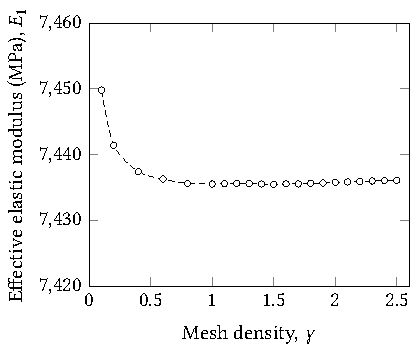
\includegraphics[scale=1]{E_sensitivity}
	%  	\hfil 	\subfloat[][Tensile strength\label{fig:TS_sens}]{\includegraphics[scale=1]{TS_sensitivity}}\\
		\caption{Mesh sensitivity of a local analysis for one realisation ($\text{SD}=20$)}
		\label{fig:mesh_sens}
	\end{figure}%

	\paragraph{Mesh sensitivity} Since element removal has an effect similar to integrating damage into the constitutive material model, mesh dependency inherently exists. Thus, to alleviate this localised deficiency, the elastic modulus of an FE prototype with the highest discrepancy ($\text{SD}=20$) was regarded. Obviously, convergence of other cases with lower SD is obtained more easily. Mesh density is defined as~\autocite{Javanbakht.2016b}
	\begin{equation}
		\gamma\equidef\frac{1}{\ell_\text{mesh}},
	\end{equation}
	where ($\ell_\text{mesh}$) is the mesh length. It is varied over a range of 0.1 to 2 to monitor the convergence behaviour. In the same manner, the auxiliary maps are also refined accordingly. As illustrated in Fig.~\ref{fig:mesh_sens}, the effective (or apparent) elastic modulus of the composite ($E_1$) gains convergence quickly with $\gamma$ over 1. In the current study, a mesh density of 1 is adopted in the analyses considering the trade-off between accuracy and efficiency.

	\paragraph{Refining auxiliary maps} In Fig.~\ref{fig:volfrac_maps}, a fibre volume fraction auxiliary map is shown. The local volume fraction is calculated as a volume average over each element, using Eq.~\eqref{eq:OTw}, and is depicted at its corresponding centre.  Thus, the corner of each pixel in the graphs correspond to the centre of an element. The mesh density controls both the refinement of finite elements and the related auxiliary maps, i.e., finer mesh requires higher resolution auxiliary maps. All the illustrated maps correspond to the same realisation with a fibre volume fraction $\zeta_\text{f}=18.88\%$. It is clear that by increasing the mesh density, a wider range of variation is captured over the domain and a more realistic visualisation of fibre distribution is obtained. 	
	
	A similar argument can be laid out for the fibre orientation distribution. In Fig.~\ref{fig:tensor_maps}, the volume-averaged orientation tensor (weighted by fibre volume) is calculated over each element and depicted along its principal direction. Moreover, the length of each fibre is scaled by the first eigenvalue of the averaged orientation tensor to show the intensity of the anisotropy. In the figures, the angle is scaled 6 times for a better presentation. The mean angle of the ODF is $7.36^\circ$ and SD of 20. It is evident that increasing the resolution of orientation auxiliary map reveals more local fluctuations since the range of angles increase from $7.49^\circ\le \varphi\le 8.17^\circ$ for $\gamma=0.1$ to $3.16^\circ\le \varphi \le13.58^\circ$ for $\gamma=1.5$.


\begin{figure}[!h]{}
  	\centering
	\subfloat[][$\gamma=0.1$\label{fig:TS_sehns}]{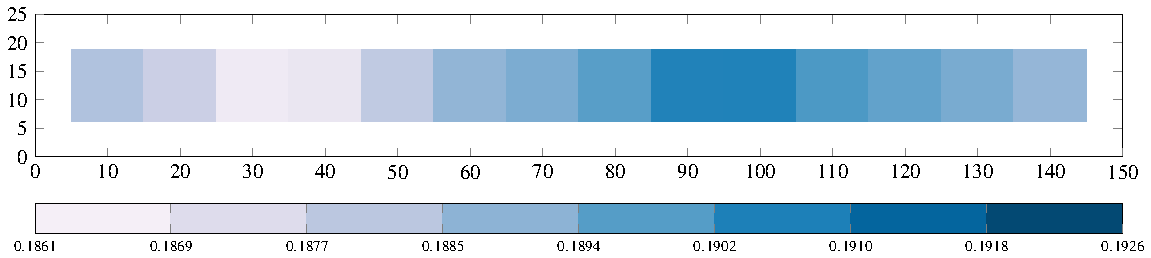
\includegraphics[width=0.9\textwidth]{volfrac_map_md100}}\\
	\subfloat[][$\gamma=0.2$\label{fig:TS_senfs}]{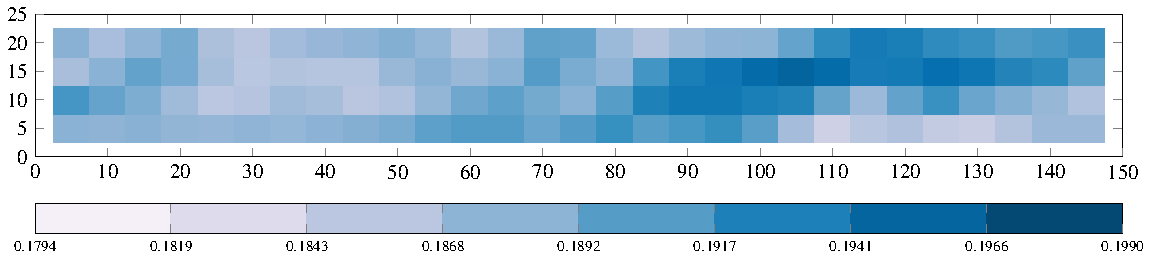
\includegraphics[width=0.9\textwidth]{volfrac_map_md200}}\\
	\subfloat[][$\gamma=0.6$\label{fig:TS_sens}]{ 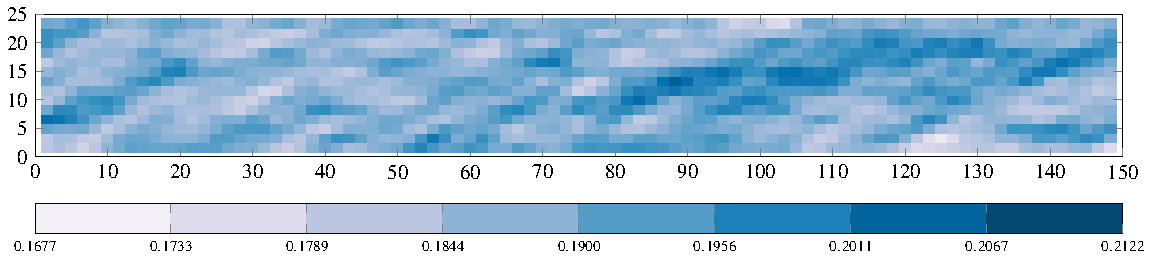
\includegraphics[width=0.9\textwidth]{volfrac_map_md600}}\\
	\subfloat[][$\gamma=1.0$\label{fig:TS_sbens}]{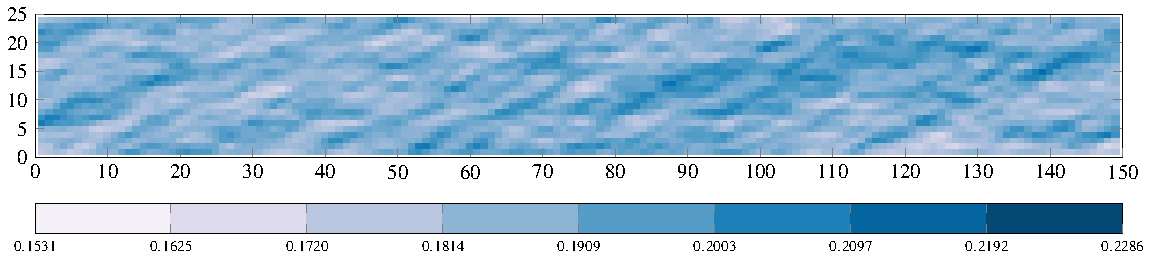
\includegraphics[width=0.9\textwidth]{volfrac_map_md1000}}\\
	\subfloat[][$\gamma=2.0$\label{fig:TS_bsens}]{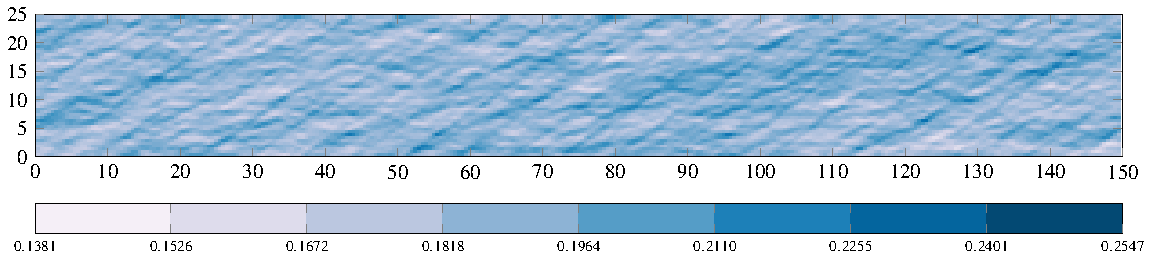
\includegraphics[width=0.9\textwidth]{volfrac_map_md2000}}
	\caption{Refining the volume fraction auxiliary map according to the mesh density for one realisation ($\text{SD}=20$)}
	\label{fig:volfrac_maps}
\end{figure}%
\afterpage{\clearpage}

\begin{figure}[!h]{}
  	\centering
	\subfloat[][$\gamma=0.1$\label{fig:S_sehns}]{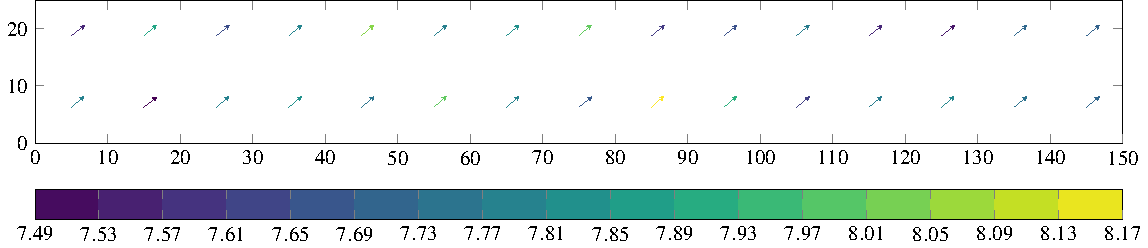
\includegraphics[width=0.9\textwidth]{tensor_map_md100}}\\
	\subfloat[][$\gamma=0.2$\label{fig:S_senfs}]{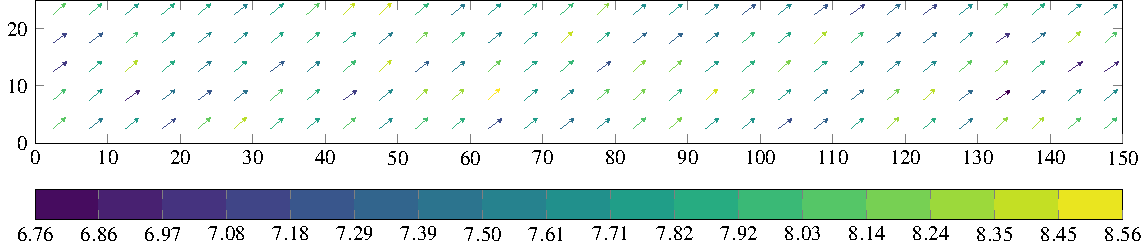
\includegraphics[width=0.9\textwidth]{tensor_map_md200}}\\
	\subfloat[][$\gamma=0.6$\label{fig:S_sens}]{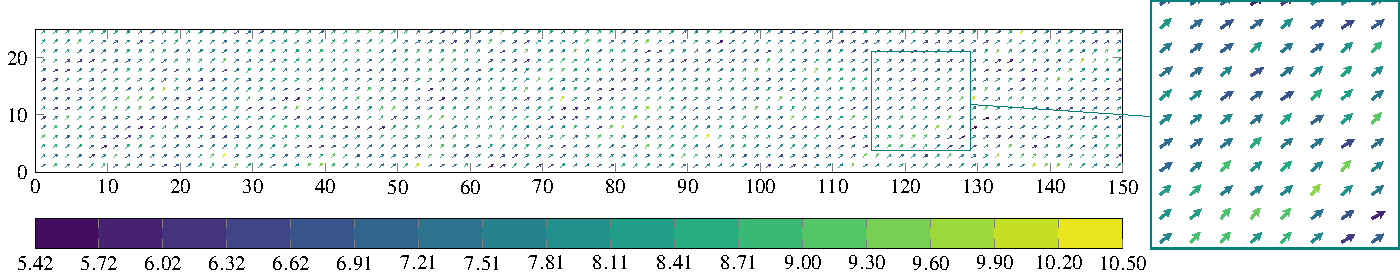
\includegraphics [width=0.9\textwidth] {tensor_map_md600}}\\
	\subfloat[][$\gamma=1.0$\label{fig:S_sbens}]{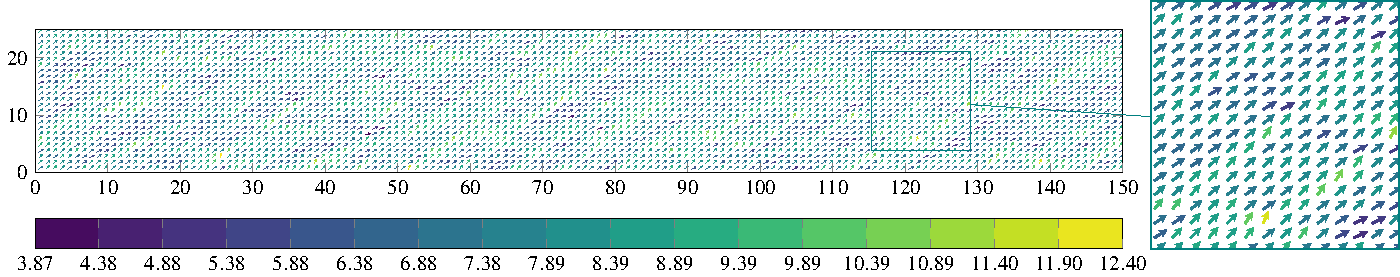
\includegraphics[width=0.9\textwidth]{tensor_map_md1000}}\\
	\subfloat[][$\gamma=1.5$\label{fig:S_bsens}]{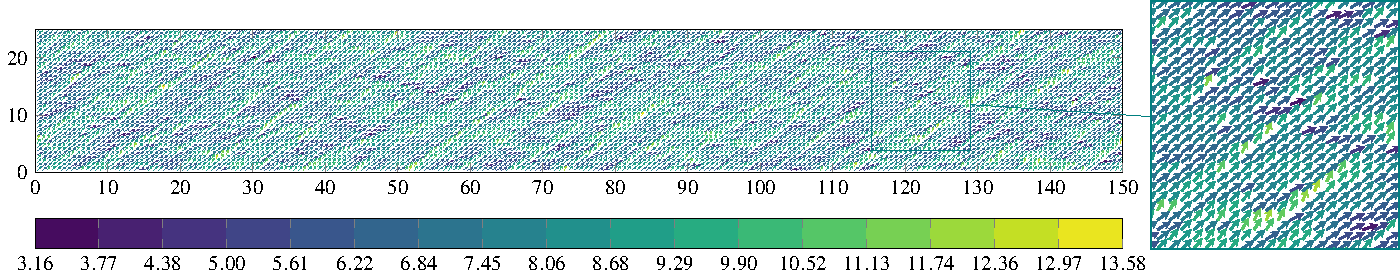
\includegraphics[width=0.9\textwidth]{tensor_map_md1500}}
	\caption{Refining the orientation tensor auxiliary map according to the mesh density for one realisation ($\text{SD}=20$); the principal directions are graphed while the angles are scaled 6 times for clarification}
	\label{fig:tensor_maps}
\end{figure}%


	\paragraph{Parametric study} The parametric study is carried out by varying the SD of the ODF, which is a Gaussian distribution as reported in~\autocite{Virk.2013}. Setting the SD to zero for the orientation distribution results in the special case of aligned fibres along the mean angle of the distribution ($7.36^\circ$). Namely, the global orientation corresponds to the local one for each element. Therefore, the first point in Fig.~\ref{fig:mesh_param} represents the global calculation that results in a mean Young's modulus of 8965.86\,MPa. Similarly, the following five points, all below $\text{SD}=5$, result in values close to the initial perfectly aligned case. The obtained results from the local analysis do not show a significant difference compared to the global value. A rather sharp drop in stiffness is observed for values over SD of 5. Moreover, the results seems to be more spread out for higher values. Interestingly, the experimental value was recorded for the SD of 17.95, which is best estimated by the local FE realisations in the range of 15--17.5. Note that the experimental value is quite distant with respect to the global value and even the local values with low SD. More specifically in Table~\ref{table:results7}, global and low-variation local Young's moduli results show relative errors of around 9\% whereas the local analysis of $\text{SD}=17.95$ contains half as much error. One could argue that based on the local FE results, the estimation of the ODF in~\autocite{Virk.2013} by the SDs in the range of 15--17.95 seems to be plausible.


\begin{figure}[!h]{}
  	\centering
  	\includegraphics[scale=1]{E_parametric}
	\caption{Parametric result of all realisations along with SD error bars; the experimental value of 8190 was reported for $\text{SD}=17.95$ in~\autocite{Virk.2013}}
	\label{fig:mesh_param}
\end{figure}%
	
	As a measure of global behaviour, Krenchel's formulation is used assuming that all the fibres are oriented along the mean angle, see Table~\ref{table:results7}. The angle is obtained from the eigenvector of the principal direction, which is the denoted by the maximum eigenvalue. The behaviour of this analytical model, along with the angle obtained from the FE analysis clearly shows that global behaviour is insensitive to local fibre orientation. This global value overestimates the experimental value by approximately 15\%.
	
	From the micromechanical point of view, focusing on local computation has a secondary benefit: the ergodicity hypothesis remains valid for each element. Thus, what is practically done is introducing an RVE for each element rather than the whole structure. Inexpensive computational cost makes this approach practical. This assumption allowed to remove an element when the scale separation hypothesis collapses due to failure---without affecting other elements.	


\begin{table}[!hb]
\centering\scriptsize
\caption{Experimental and numerical results for the effective elastic modulus of the composite ($E_1$, in MPa), and relative error in percentage}\label{table:results7}
\begin{tabular}{l@{\hspace{0.1cm}}l@{}*{11}{c}}
\toprule
\multicolumn{2}{l}{\multirow{2}{*}{\bfs{Composite property}}}  &  \multicolumn{11}{c}{\bfs{Standard deviation of angle distribution}} \\                                                           
\cmidrule(l{0cm}r{0cm}){3-13} && \hfil\bfs{0}&\hfil\bfs{1}&\hfil\bfs{2}&\hfil\bfs{3}&\hfil\bfs{4}&\hfil\bfs{5}&\hfil\bfs{10}&\hfil\bfs{15}&\hfil\bfs{17.5}&\hfil\bfs{17.95}& \hfil\bfs{20}\\	
\toprule
%\multirow{3}{*}{$E_\text{Local}$}& Mean (MPa)			&8965.86	&8958.61 &8897.15	&8940.65 &8903.21 &8905.26&8567.98 &8074.07	&7795.04 &7805.69 &7403.08\\
% The previous line was change to the following to keep the same number of significant digits for both values and their SDs.
\multirow{3}{*}{$E_\text{Local}$}& Mean (MPa)			&8966	&8959 &8897	&8941 &8903 &8905&8568 &8074&7795 &7806 &7403\\
%					&SD (MPa)				&23.33	&53.76   &74.20	    &26.65	 &42.32	  &120.40 &	135.48 &98.19	&381.70	 & 215.77 &264.99\\
					&SD (MPa)				&23.33	&53.76   &74.20	    &26.65	 &42.32	  &120.4 &	135.5 &98.19	&381.7	 & 215.8 &264.9\\
&Relative error (\%) &9.47    &9.38      &8.63	 &9.17	  &8.71   &8.73	   &4.62	&1.42	 &4.82	  &4.69	&10.13\\\midrule
\multirow{2}{*}{$\theta_\text{Global}$}&Mean   &7.36&7.41&7.59&7.17&7.29&7.41&7.27&7.39&7.56&6.79&8.23\\
&SD&0.00&0.25&0.40&0.13&0.24&0.17&0.97&0.42&1.81&1.56&1.41\\\midrule
%\multirow{2}{*}{$E_\text{Global}$}&Krenchel (MPa) & 9386.08&	9382.99&9370.84& 9398.16&9390.46&9382.87 &9392.08 &9383.88 &9372.93&9421.69 &9325.91\\
\multirow{2}{*}{$E_\text{Global}$}&Krenchel (MPa) & 9386.08&	9383&9371& 9398&9391&9383 &9392 &9384 &9373&9422 &9326\\
&Relative error (\%)  &14.60&14.57&14.42&14.75&14.66&14.56&14.68&14.58&14.44&15.04&13.87\\
 \bottomrule
\end{tabular}
\end{table}
	
	Obviously, the discussion is based on the few number of realisations. More accurate results could be obtained by increasing the number of realisations to better approximate the ensemble value. Namely, more realisations may decrease the variation of the output but it would not violate the overall observed behaviour.
	


\section{Conclusion}	
	The focus of this work was on developing a simple element-wise semi-numerical scheme to homogenise aligned NFRCs through a cost-effective approach. To this end, after reviewing the concept of orientation tensor and presenting the pertaining constitutive equation, the following points were motivated to consider auxiliary maps:
%	with the potential to be incorporated  multi-scale simulations.
	\begin{itemize}
		\item Local anisotropy (more specifically transverse isotropy for the case of long fibres) and its global counterpart were distinguished from each other. In the former, the elastic stiffness acquires a point-wise transverse symmetry for which the axis of symmetry is a function of location whereas in the latter insensitivity to the local variation is evident.
		\item Accepting the ergodic hypothesis for a material requires statistical homogeneity of its micro-structure (even when random heterogeneities are present). Fulfilling such a condition for the whole structure is quite strong but demanding it element-wisely relaxes the requirements.
	\end{itemize}
	The effective elastic modulus of NFRCs of an experimental study was predicted. Mesh dependency of the results was quickly removed by refining the elements while the auxiliary maps were scaled down to the same extent. It was observed that increasing the SD of ODF over values of 5 highly reduces the effective stiffness of the sample. While lower values of SD overestimated the experimental result, higher values (around the reported SD of the ODF) give plausible estimates within 5\% error range in average. Analytical approach that considers the global average orientation, remained insensitive to local variation.
		
	Based on the obtained results, the following points are suggested:
	\begin{itemize}
		\item Instead of the more common global or layer-wise calculation of the orientation tensor, an element-wise approach should be adopted (where possible). The proposed procedure is in accordance with subdividing the whole structure to finite elements as auxiliary maps followed the same refinement. In addition, auxiliary maps of volume fraction and orientation tensor enabled setting up an independent RVE for each element. 
		\item It was shown that mesh-independent results were obtained using auxiliary maps and through a 2D simple analysis. Namely, projecting all layers onto a single 2D layer does not include much loss of information in regard to orientation. This could be a good recommendation that as a result of specific manufacturing techniques, 3D computation is bypassed. 
	\end{itemize}
	By implementing the suggestions of the current study, adequate local morphological information was captured and a more accurate, yet computationally inexpensive, simulation of mechanical response was carried out.	

	\paragraph{Future work} Auxiliary map(s) of clustering index and/or damage might be used in conjunction with the introduced maps of the current study to elaborate the understanding of  material response in future works. A comparison between the local and global failure criteria should be carried out to challenge the proposed method in strength calculations---specially when element removal is involved.


    %!TeX spellcheck = en_GB
%!TEX TS-program = xelatex
%!BIB TS-program = biber

\chapter{Concluding Remarks}\label{chap:conc}

\paragraph{Key findings} The key findings of the conducted research can be summarised as follows:

% contingency measure

\begin{enumerate}[label=Stage~\Roman*.]
	\item 
	\begin{itemize}
		\item The effective thermal conductivity of discontinuous FRCs is improved by increasing the fibre volume fraction. The deviation of the values is highly dependant on the randomness of the fibre generation procedure. Discrete fibre elements can easily capture these aspects by means of the FEA. 
		\item At higher volume fractions, the sensitivity of the effective properties to mesh density becomes more sensible. Thus, a sensitivity analysis is recommended for non-dilute FRCs. The fibre efficiency depends on the fraction of fibres that are oriented along the temperature gradient. Moreover, one must distinguish between the nominal and true fibre volume fractions when dealing with discrete fibre elements since these values do not always correspond. The deviation becomes highly pronounced at higher volume fractions.
		\item In modelling the hygroscopic effects of natural fibres, distinguishing between the technical and elemental fibres can be detrimental. The thermal conductivity of saturated natural fibres increases by increasing the porosity of the fibres whereas in the absence of moisture, conductivity diminishes.
	\end{itemize}
	\item 
	\begin{itemize}
		\item In randomly-oriented discontinuous FRCs, which are generated by pseudo-random fibre generation, the fibre volume fraction alters the thermal conductivity more than the clustering effects. However, the non-uniform distribution of the fibres causes a local resistance barrier against conductivity. Spectral analysis of the orientation tensor could be used to detect the principal direction of the fibres but the results of clustering index could not completely relate to conductivity. More localised investigation of the clustering is recommended.
		\item It was found that orienting the principal direction of fibres along the heat gradient increases the effective conductivity provided that clustering is minimum. The degree of anisotropy of the composite increases as the maximum eigenvalue of the orientation tensor becomes closer to unity. Moreover, spectral analysis seems to be more sensitive to orientation than the clustering index. Thus, spectral analysis of the orientation tensor could aid in determining the fibre efficiency in the thermal and mechanical analyses.
	\end{itemize}
	\item 
	\begin{itemize}
		\item Assuming a perfect circular cross-section for fibres, results in underestimation of elastic properties, and thus analytical bounding models should be rectified by the FACF. Moreover, modelling technical fibres as discrete finite elements also necessitates a similar amendment. Implicit modelling of damage can be carried out by removing the fibre/matrix finite elements upon failure. The element elimination technique was extended to simulating NFRCs with embedded elements. This incorporates a softening effect into the effective elastic modulus of the FRC, and thus a non-linear behaviour is artificially induced without having any available data on damage. In order to deal with the failure strength, one should acquire a fracture mechanical point of view, i.e., to consider that shorter fibres are stronger; this argument is also backed up by statistical data from experiments. It is recommended that the strength of fibres must be updated upon a partial failure in a way that the remaining shortened portion of the original fiber attains a higher failure stress. Although this updating does not affect the effective elasticity, the failure strength of the NFRCs approaches the experimental values.
		\item The concept of auxiliary maps is introduced, which is map containing localised data. By means of a semi-numerical element-wise scheme it was shown that linking the mesh density to the resolution of auxiliary maps results in the quick convergence of effective elasticity. Furthermore, unlike spectral analysis, the derived formulation seems to be sensitive to localised data. This feature could be linked to the use of the orientation tensor auxiliary map with an appropriate resolution. Moreover, the model is capable of incorporating the element removal framework for damage modelling. From a micro-mechanical point of view, this capability differs from other models since elements are not linked to a single RVE but instead, each element has its own separate localised model. Overall, the use of auxiliary maps is recommended against the more common global or layer-wise calculations. It was shown that mesh-independent results were obtained using auxiliary maps and through a very cost effective equivalent 2D analysis. This could be a good recommendation that as a result of specific manufacturing techniques, 3D computations could be bypassed. The application of the developed method was carried out for NFRCs but could be applied to any type of FRCs. Namely, provided that adequate local morphological information exists, the computationally inexpensive simulation of mechanical response could be carried out for any type of FRCs. To this end, an in-house portable program is developed that carries out prototyping, pre- and post-analyses, automatically.
	\end{itemize}
\end{enumerate}
	
	\paragraph{Future work} The final stages of the current work lays a solid understanding of the mechanical response of NFRCs that could potentially be extended to other types of FRCs. More specifically, the following ideas could be pursued:
	\begin{itemize}
		\item Auxiliary maps of clustering index and/or damage might be used in conjunction with the introduced models to elaborate the understanding of the material response in future works. A comparison between the local and global failure criteria should be carried out to challenge the proposed method in strength calculations---specially when element removal is involved.
		\item The strength-updating procedure could be implemented analytically in the model.
		\item The introduced method can be used in multi-scale modelling to set up a simple RVE with embedded fibres in the meso-scale. 
		\item An explicit damage parameter could be included in the model by including the isotropic/anisotropic damage tensor.
		\item In addition, the element elimination scheme could be further improved by considering a non-local continua formulation, such as the non-local strain field, to make the damage propagation smoother and alleviate the artificial stress concentration due to the sudden fibre removal.
		\item The development of an invariant formulation in terms of higher order orientation tensor could be investigated.
	\end{itemize}

			

%\appendix
%% !TEX TS-program = xelatex
% !TeX spellcheck = en\_GB
% !TeX root = ../My_thesis.tex

\chapter{Tensor Identities}

\begin{equation}
\diver{\,(\tena{v}\cross\tenb{T})}\equiv (\curl{\tena{v}})\scp\tenb{T}-\tena{v}\scp(\curl{\tenb{T}})
\end{equation}

\begin{equation}
\diver{\,(\tenb{T}\cross\tena{v})}\equiv (\diver{\tenb{T}})\cross\tena{v}+  \tenb{T}^\tran\scpcross\grad{\tena{v}}\label{eq:divercross1}
\end{equation}

\begin{equation}
\begin{aligned}
\diver{\,(\tend{A}\dscp\tenb{B})}&\equiv(\diver{\tend{A}})\dscp\tenb{B}+\tend{A}^\ltran\tscp\grad{\tenb{B}}\\
                                 &\equiv(\diver{\tend{A}})\dscp\tenb{B}+\grad{\tenb{B}}\dscp\kern-0.6ex\scp\tend{A}^\tran
\end{aligned}
\end{equation}
Leibniz's product rule:
    \begin{subequations}
    \begin{alignat}{3}
               \diver{\,(\tenb{A}\alpha)}&\equiv(\diver{\tenb{A}})\alpha+\tenb{A}\scp\grad{\alpha},\\
    \diver{\,(\tenb{A}\scp\tena{v})}&\equiv(\diver{\tenb{A}})\scp\tena{v}+\tenb{A}\dscp\grad{\tena{v}},\\
    \diver{\,(\tenb{A}\scp\tenb{B})}&\equiv(\diver{\tenb{A}})\scp\tenb{B}+\tenb{A}\dscp\grad{\tenb{B}}.
    \end{alignat}
    \end{subequations}
    
    \begin{alignat}{3}
    \grad{(\tena{u}\dyad\tena{v})}\equiv(\grad{\tena{u}})\dyad\tena{v}+(\grad{\tena{v}})\dyad\tena{u}
    \end{alignat}

    \begin{equation}
    \diver{\tena{v}}=\tr{(\grad{\tena{v}})}
    \end{equation}


Gauss-Ostrogradsky's theorem followed by its corollaries:
    \begin{subequations}
    \begin{alignat}{2}
        \int_\Omega \alpha\, \partial_i \beta\dV 
            +\int_\Omega \beta\, \partial_i \alpha\dV 
            &=\int_{\partial\Omega} \alpha\beta n_i \dS,\\
        \int_\Omega \grad{\alpha} \dV 
            &=\int_{\partial\Omega} \alpha\tena{n} \dS,\\
        \int_\Omega \grad{\tena{v}} \dV 
            &=\int_{\partial\Omega} \tena{n}\dyad \tena{v} \dS,\\
        \int_\Omega \diver{\tena{v}} \dV 
            &=\int_{\partial\Omega} \tena{n}\scp \tena{v} \dS,\\\label{eq:GOdiv}
        \int_\Omega \curl{\tena{v}} \dV 
            &=\int_{\partial\Omega} \tena{n}\cross\tena{v} \dS,\\
        \int_\Omega \grad{\tenb{A}} \dV 
            &=\int_{\partial\Omega} \tena{n}\dyad \tenb{A} \dS,\\
        \int_\Omega \ten{A}\dyad\grad{\ten{B}} \;\dif V 
            + \int_\Omega \grad{\ten{A}}\dyad\ten{B}\; \dif V 
            &=\int_{\partial\Omega} \tena{n}\dyad\ten{A}\dyad\ten{B} \;\dif S,\\ 
        \int_\Omega \grad{\ten{A}}\;\dif V 
            &= \int_{\partial\Omega} \tena{n}\dyad\ten{A} \;\dif S
    \end{alignat}
    \end{subequations}
Equation \eqref{eq:GOdiv} is used to obtain Green's identities 1--4 by defining a vector field $\tena{v}\equidef \phi\grad{\psi}$ using two scalar fields $\psi$ and $\phi$:
    \begin{subequations}
    \begin{alignat}{2}
        \int_\Omega \grad{\phi}\scp\grad{\psi} + \phi\lap{\psi} \dV 
            &=\int_{\partial\Omega} \tena{n}\scp  \phi\grad{\psi}\dS,\\
        \int_\Omega \phi\lap{\psi} - \psi\lap{\phi} \dV 
            &=\int_{\partial\Omega} \tena{n}\scp(\phi\grad{\psi}-\psi\grad{\phi})\dS,\\
        \int_\Omega \norm{\grad{\psi}}^2 - \psi\lap{\psi} \dV 
            &=\int_{\partial\Omega} \tena{n}\scp\psi\grad{\psi}\dS,\\
    \end{alignat}
    \end{subequations}
%% !TEX TS-program = xelatex
% !TeX spellcheck = en\_GB
% !TeX root = ../My_thesis.tex

\chapter{From Tensor to Matrix}
	In the case of left- and right-minor symmetries and major symmetry of a fourth-order tensor, a bijective transformation between  the $\Real^3\times\Real^3\times\Real^3\times\Real^3\times$ space and the $\Real^6\times\Real^6$ symmetric matrix space. The most typical notation would be that of the Voigt's. In order to retain the same behaviour under inner product, some coefficients are added to amend this deficiency of Voigt's notation that gives rise to Mandel's notation.
\begin{subequations}
\begin{alignat}{2}
	\unitb\dyad\unitb=&
	\begin{bmatrix}
	1&1&1&0&0&0\\
	1&1&1&0&0&0\\
	1&1&1&0&0&0\\
	0&0&0&0&0&0\\
	0&0&0&0&0&0\\
	0&0&0&0&0&0\\
	\end{bmatrix},\\
	\unitb\dyadd\unitb=&
	\begin{bmatrix}
	1&0&0&0&0&0\\
	0&1&0&0&0&0\\
	0&0&1&0&0&0\\
	0&0&0&1&0&0\\
	0&0&0&0&1&0\\
	0&0&0&0&0&1\\
	\end{bmatrix}.
\end{alignat}
\end{subequations}
% ══════════════════════════════════════════════════════════════════════════════════════════════════
\newpage
\printbibliography[title=References,heading=bibintoc]

% ══════════════════════════════════════════════════════════════════════════════════════════════════

\end{document}
